\documentclass[11pt, a4paper, twoside]{article}
\usepackage[T1]{fontenc}
\usepackage[utf8]{inputenc}
\usepackage{amssymb,amsmath}
\usepackage[portuguese]{babel}
\usepackage{comment}
\usepackage{datetime}
\usepackage[pdfusetitle]{hyperref}
\usepackage[all]{xy}
\usepackage{graphicx}
\addtolength{\parskip}{.5\baselineskip}

%aqui comeca o que eu fiz de verdade, o resto veio e eu to com medo de tirar
\usepackage{xcolor}
\usepackage{listings} %biblioteca pro codigo
\usepackage{color}    %deixa o codigo colorido bonitinho
\usepackage[landscape, left=0.5cm, right=0.5cm, top=1cm, bottom=1.5cm]{geometry} %pra deixar a margem do jeito que o brasil gosta

\definecolor{gray}{rgb}{0.4, 0.4, 0.4} %cor pros comentarios
%\renewcommand{\footnotesize}{\small} %isso eh pra mudar o tamanho da fonte do codigo
\setlength{\columnseprule}{0.2pt} %barra separando as duas colunas
\setlength{\columnsep}{10pt} %distancia do texto ate a barra

\lstset{ %opcoes pro codigo
breaklines=true,
keywordstyle=\color{blue}\bfseries,
commentstyle=\color{gray},
breakatwhitespace=true,
language=C++,
%frame=single, % nao sei se gosto disso ou nao
numbers=none,
rulecolor=\color{black},
showstringspaces=false
stringstyle=\color{blue},
tabsize=4,
basicstyle=\ttfamily\footnotesize, % fonte
}
\lstset{literate=
%   *{0}{{{\color{red!20!violet}0}}}1
%    {1}{{{\color{red!20!violet}1}}}1
%    {2}{{{\color{red!20!violet}2}}}1
%    {3}{{{\color{red!20!violet}3}}}1
%    {4}{{{\color{red!20!violet}4}}}1
%    {5}{{{\color{red!20!violet}5}}}1
%    {6}{{{\color{red!20!violet}6}}}1
%    {7}{{{\color{red!20!violet}7}}}1
%    {8}{{{\color{red!20!violet}8}}}1
%    {9}{{{\color{red!20!violet}9}}}1
%	 {l}{$\text{l}$}1
	{~}{$\sim$}{1} % ~ bonitinho
}

\title{Voce beijaria Matheus Leal Viana? \\ UFMG}
\author{Naim Santos, Tiago Domingos e Yan Silva}


\begin{document}
\twocolumn
\date{\today}
\maketitle


\renewcommand{\contentsname}{Índice} %troca o nome do indice para indice
\tableofcontents


%%%%%%%%%%%%%%%%%%%%
%
% dp
%
%%%%%%%%%%%%%%%%%%%%

\section{dp}

\subsection{DivideConquer.cpp}
\begin{lstlisting}
Hash: eb41c6
/* Source: cp-algorithms
 * Complexity: O(N*K*log(N)*cost())
 * Needs to be monotonic
 * !! compute(1,n,1,n) vs compute(i,n,i,n)  
 * Usefull Strat: if is difficult to precompute all cost, one can use two pointers
 * Similar to MO's algorithm, resulting in O(K*Nlog\N) complexity, up only by a constant factor.
*/
24 24 struct DP{
9f 5e 	int n , inf; 
a6 9e 	vi dp[2];
2c f5 	DP(int n , int inf) : n(n) , inf(inf) {dp[0] = vi(n+1) , dp[1] = vi(n+1);}
b2 03 	int cost(int i,int j);
      	// compute dp_cur[l], ... dp_cur[r] (inclusive) 
9f be 	void compute(int l, int r, int optl, int optr){
ce de 	    if (l > r) return;
1d 31 	    int mid = l + (r-l)/2;
f4 25 	    pair<int, int> best = {inf, -1}; // se for maximizar muda pra -inf
61 bd 	    rep(k,optl,min(mid,optr)+1){
b8 67 	        best = min(best, { dp[0][k-1] + cost(k,mid), k});
c1 cb 	    }
d8 68 	    dp[1][mid] = best.first; int opt = best.second;
fd f9 	    compute(l, mid - 1, optl, opt);
e4 5c 	    compute(mid + 1, r, opt, optr);
98 cb 	}
a1 d1 	void solve(int k){
b4 04 		rep(i,1,n+1){
96 ed 			dp[0][i] = cost(1,i);
63 cb 		}
c4 ff 		rep(i,2,k+1){
60 01 			rep(j,i,n+1) dp[1][j] = inf;
ed 6c 			compute(i,n,i,n) ;
a6 f1 			swap(dp[0] , dp[1]);
35 cb 		}
95 cb 	}
eb 21 };
\end{lstlisting}

\subsection{Knuth.cpp}
\begin{lstlisting}
Hash: c65320
2b 2b #include <bits/stdc++.h>
91 ca using namespace std;
36 ad typedef long long ll;
3a 6e const int N = 5005;
b9 05 ll s[N] , dp[N][N];
d0 20 int opt[N][N] , n;
 
 
 
83 c6 int32_t main(){
52 f4 	scanf("%d" , &n);
ae 78 	for(int i = 1 ; i <= n; i ++){
1d d5 		scanf("%lld" , &s[i]);
d9 78 		s[i] += s[i-1];
47 24 		dp[i][i] = 0 , opt[i][i] = i;
78 cb 	}
ac 78 	for(int len = 2; len <= n; len ++){
64 21 		for(int i = 1 , j = len ; j <= n; i ++ , j ++){
1f 0e 			dp[i][j] = s[j] - s[i-1] + dp[i][opt[i][j-1]] + dp[opt[i][j-1] + 1][j];
65 ce 			opt[i][j] = opt[i][j-1];
7e 60 			for(int k = opt[i][j-1]  ; k <= opt[i+1][j] ; k ++){
64 a8 				if(dp[i][j] > (s[j] - s[i-1]) + dp[i][k] + dp[k+1][j]){
ef 14 					opt[i][j] = k;
ad 65 					dp[i][j] = s[j] - s[i-1] + dp[i][k] + dp[k+1][j];
7c cb 				}
8a cb 			}
19 cb 		}
03 cb 	}
a8 fd 	printf("%lld\n" , dp[1][n]);
c6 cb }
\end{lstlisting}



%%%%%%%%%%%%%%%%%%%%
%
% number-theory
%
%%%%%%%%%%%%%%%%%%%%

\section{number-theory}

\subsection{CrivoSegmentado.cpp}
\begin{lstlisting}
Hash: 09db86
/* Author: Common knowledge
 * Description: Crivo para decompor numeros no range [L,R] , R<=10^12 para casos de R-L pequeno i.e R-L<=1e6
 * Precisa precomputar os primos menores que sqrtR com outro crivo
 * Apos o crivo, mark[i-l] tem 1 se i nao for primo, caso contrario, mark[i-l] eh um primo.
 * Status: Tested on Petrozavodsk Summer-2017. Songyang Chen Contest 1 - problem C
 */
1a 1a const int N = 1e6 + 100; // N>=sqrt(MaxR)
76 98 bool mark[N];
eb 38 vi pr;
93 7a void crivo_segmentado(ll l,ll r){
      	//crivo(); jogando primos em pr
        
64 16 	for(ll i = l;i<=r;i++){
bb e7 		mark2[i-l] = i;
1a 54 		ans[i-l] = 1;
09 cb 	}
      
42 02 	for(ll p : pr){
      	  
75 da 		for(ll i = (l + p -1)/p * p ;i<=r;i+=p){
96 a1 			ll cnt =0;
3a f7 			while(mark2[i-l]%p==0){
33 5c 				mark2[i-l]/=p;
52 f6 				cnt++;
d9 cb 			}
aa 93 			ans[i-l] = ans[i-l]*(cnt + 1)%M; // exemplo -> qtd de divisores de i
01 cb 		}
c2 cb 	}
      	
7f 16 	for(ll i = l;i<=r;i++){
13 30 	  if(mark2[i-l]!=1){//eh um primo > Sqrt
4e d4 		ans[i-l] = ans[i-l] * (1 + 1) %M;    
41 cb 	  }
ed cb 	}
        
09 cb }
\end{lstlisting}

\subsection{Crt.cpp}
\begin{lstlisting}
Hash: e40708
/* Source: Aeren's library
 * Description: Chinese Remainder Theorem (Return a number x which satisfies x = a mod m & x = b mod n)
 * All the values has to be less than 2^30
 * Retorna o menor X >=0 que satisfaz ou -1 se nao tem resposta
 * a1 + b1 * k1 == a2 + b2 * k2 -> (a1-a2)== -b1*x + b2*y
 * Isso vira uma equacao diofantina.
 * Time: O(log(N + M)
 * the resulting modulo is LCM(n,m)
 * Status: tested on kattis
 */
ad ad typedef long long ll;
0f 9d ll euclid(ll x, ll y, ll &a, ll &b){
d6 ce 	if(y){
39 11 		ll d = euclid(y, x % y, b, a);
94 2c 		return b -= x / y * a, d;
c8 cb 	}
0a 13 	return a = 1, b = 0, x;
96 cb }
7c b5 ll crt_coprime(ll a, ll m, ll b, ll n){
3b 53 	ll x, y; euclid(m, n, x, y);
30 6e 	ll res = ( a * (y + m) % m ) * n + ( b * (x + n) % n ) * m;
a8 0f 	if(res >= m * n) res -= m * n;
96 b5 	return res;
13 cb }
0d 24 ll crt(ll a, ll m, ll b, ll n){
e3 04 	ll d = gcd(m, n);
e4 09 	if(((b -= a) %= n) < 0) b += n;
f4 ba 	if(b % d) return -1; // No solution
a1 8f 	return d * crt_coprime(0LL, m/d, b/d, n/d) + a;
e4 cb }
\end{lstlisting}

\subsection{Diofantina.cpp}
\begin{lstlisting}
Hash: 87b1ec
89 89 int gcd(int a, int b, int& x, int& y) {
3d a3     if (b == 0) {
14 48         x = 1;
18 01         y = 0;
ad 3f         return a;
cc cb     }
2e 60     int x1, y1;
1b e8     int d = gcd(b, a % b, x1, y1);
97 71     x = y1;
a4 a2     y = x1 - y1 * (a / b);
67 be     return d;
af cb }

0a 36 bool find_any_solution(int a, int b, int c, int &x0, int &y0, int &g) {
38 33     g = gcd(abs(a), abs(b), x0, y0);
b0 a9     if (c % g) {
54 d1         return false;
fd cb     }
      
25 21     x0 *= c / g;
7b 47     y0 *= c / g;
c5 8c     if (a < 0) x0 = -x0;
b4 1f     if (b < 0) y0 = -y0;
06 8a     return true;
50 cb }

e2 08 void shift_solution(int & x, int & y, int a, int b, int cnt) {
72 52     x += cnt * b;
ea fd     y -= cnt * a;
93 cb }

4e f0 int find_all_solutions(int a, int b, int c, int minx, int maxx, int miny, int maxy) {
09 ed     int x, y, g;
8b 79     if (!find_any_solution(a, b, c, x, y, g))
22 bb         return 0;
a4 fe     a /= g;
ba ee     b /= g;
      
0f 07     int sign_a = a > 0 ? +1 : -1;
8a f8     int sign_b = b > 0 ? +1 : -1;
      
38 ab     shift_solution(x, y, a, b, (minx - x) / b);
f1 59     if (x < minx)
10 8a         shift_solution(x, y, a, b, sign_b);
92 6b     if (x > maxx)
f0 bb         return 0;
3e 57     int lx1 = x;
      
5a 98     shift_solution(x, y, a, b, (maxx - x) / b);
88 6b     if (x > maxx)
b6 f6         shift_solution(x, y, a, b, -sign_b);
8e eb     int rx1 = x;
      
52 76     shift_solution(x, y, a, b, -(miny - y) / a);
5f a6     if (y < miny)
67 bf         shift_solution(x, y, a, b, -sign_a);
6d a1     if (y > maxy)
53 bb         return 0;
4e 8e     int lx2 = x;
      
b5 e3     shift_solution(x, y, a, b, -(maxy - y) / a);
11 a1     if (y > maxy)
85 b1         shift_solution(x, y, a, b, sign_a);
d4 48     int rx2 = x;
      
27 47     if (lx2 > rx2)
16 e7         swap(lx2, rx2);
2b 2b     int lx = max(lx1, lx2);
01 03     int rx = min(rx1, rx2);
      
9f f0     if (lx > rx)
20 bb         return 0;
78 eb     return (rx - lx) / abs(b) + 1;
87 cb }
\end{lstlisting}

\subsection{DiscreteRoot.cpp}
\begin{lstlisting}
Hash: a61909
/**
 * Author: cp-algorithms
 * Date: 2020-01-11
 * Description: Resolver equacoes do tipo x^k = a (mod N) onde x eh a variavel (k,a,N) sao dados
 * Retorna todas as solucoes 
 * Cuidado com o caso a = 0. Colocar Long long se for necessario
 * Time: O(ans * log^2(N))
 * Status:tested
 */
 
b7 b7  struct DiscreteRoot{
      	/*
      		OBS: Se for necessario Use LONG LONG
      	*/
88 ba 	int gcd(int a, int b) {
ba e3 	    return a ? gcd(b % a, a) : b;
01 cb 	}
      
98 61 	int powmod(int a, int b, int p) {
20 c9 	    int res = 1;
2d 63 	    while (b > 0) {
13 2c 	        if (b & 1) {
f1 dc 	            res = res * a % p;
6a cb 	        }
48 cd 	        a = a * a % p;
46 1b 	        b >>= 1;
81 cb 	    }
4c b5 	    return res;
99 cb 	}
      
      	// Finds the primitive root modulo p
62 e4 	int generator(int p) {
c7 99 	    vector<int> fact;
d8 73 	    int phi = p-1, n = phi;
60 3e 	    for (int i = 2; i * i <= n; ++i) {
e4 c0 	        if (n % i == 0) {
1d a5 	            fact.push_back(i);
bc 49 	            while (n % i == 0)
53 13 	                n /= i;
47 cb 	        }
2d cb 	    }
40 f3 	    if (n > 1)
da d2 	        fact.push_back(n);
      
70 a5 	    for (int res = 2; res <= p; ++res) {
01 97 	        bool ok = true;
de 2c 	        for (int factor : fact) {
e7 39 	            if (powmod(res, phi / factor, p) == 1) {
31 98 	                ok = false;
9d c2 	                break;
4b cb 	            }
68 cb 	        }
cb 97 	        if (ok) return res;
de cb 	    }
19 da 	    return -1;
9d cb 	}
      
      	// This program finds all numbers x such that x^k = a (mod n)
ae b3 	vector<int> solve(int n, int k, int a){
73 22 		if(a==0){
be 37 			return {1};
21 cb 		}
      
37 a9 	    int g = generator(n);
      
      	    // Baby-step giant-step discrete logarithm algorithm
ae 2b 	    int sq = (int) sqrt (n + .0) + 1;
25 58 	    vector<pair<int, int>> dec(sq);
ef 35 	    for (int i = 1; i <= sq; ++i)
a3 b7 	        dec[i-1] = {powmod(g, i * sq * k % (n - 1), n), i};
be b3 	    sort(dec.begin(), dec.end());
88 98 	    int any_ans = -1;
7d 91 	    for (int i = 0; i < sq; ++i) {
f8 6d 	        int my = powmod(g, i * k % (n - 1), n) * a % n;
9f 40 	        auto it = lower_bound(dec.begin(), dec.end(), make_pair(my, 0));
e3 34 	        if (it != dec.end() && it->first == my) {
1a b2 	            any_ans = it->second * sq - i;
48 c2 	            break;
8e cb 	        }
93 cb 	    }
b1 d0 	    if (any_ans == -1) {
93 21 	        return {};
de cb 	    }
      
      	    // Print all possible answers
98 d7 	    int delta = (n-1) / gcd(k, n-1);
ed da 	    vector<int> ans;
6c e4 	    for (int cur = any_ans % delta; cur < n-1; cur += delta){
9c ff 	        ans.push_back(powmod(g, cur, n));
5f cb 	    }
      
e5 d2 	    sort(ans.begin(), ans.end());
aa ba 	    return ans;
65 cb 	}
a6 21 };
\end{lstlisting}

\subsection{DivisionTrick.cpp}
\begin{lstlisting}
Hash: 5bf9bf
// by tfg50 - floor(n/i) business in sqrt(N)
79 79 for(int l = 1, r; l <= n; l = r + 1) {
3f 74 	r = n / (n / l);
      	// n / i has the same value for l <= i <= r
5b cb }
// Pra ceil(n/i) eh os mesmos intervalos com uma margem de erro de +-1
// Tanto pro L quanto pro R.
\end{lstlisting}

\subsection{Euclid.cpp}
\begin{lstlisting}
Hash: ee6239
/**
 * Author: Unknown
 * Date: 2002-09-15
 * Source: predates tinyKACTL
 * Description: Finds two integers $x$ and $y$, such that $ax+by=\gcd(a,b)$. If
 * you just need gcd, use the built in \texttt{\_\_gcd} instead.
 * If $a$ and $b$ are coprime, then $x$ is the inverse of $a \pmod{b}$.
 */

c2 c2 ll euclid(ll a, ll b, ll &x, ll &y) {
82 b8 	if (b) { ll d = euclid(b, a % b, y, x);
2c b0 		return y -= a/b * x, d; }
be 4c 	return x = 1, y = 0, a;
ee cb }
\end{lstlisting}

\subsection{Factor.cpp}
\begin{lstlisting}
Hash: 8986ac
/**
 * Author: chilli, SJTU, pajenegod
 * Date: 2020-03-04
 * License: CC0
 * Source: own
 * Description: Pollard-rho randomized factorization algorithm. Returns prime
 * factors of a number, in arbitrary order (e.g. 2299 -> \{11, 19, 11\}).
 * Time: $O(n^{1/4})$, less for numbers with small factors.
 * Status: stress-tested
 *
 * Details: This implementation uses the improvement described here
 * one can accumulate gcd calls by some factor (40 chosen here through
 * exhaustive testing). This improves performance by approximately 6-10x
 * depending on the inputs and speed of gcd. Benchmark found here:
 *
 * GCD can be improved by a factor of 1.75x using Binary GCD
 * However, with the gcd accumulation the bottleneck moves from the gcd calls
 * to the modmul. As GCD only constitutes ~12% of runtime, speeding it up
 * doesn't matter so much.
 *
 * This code can probably be sped up by using a faster mod mul - potentially
 * montgomery reduction on 128 bit integers.
 * Alternatively, one can use a quadratic sieve for an asymptotic improvement,
 * which starts being factor in practice around 1e13.
 *
 * Brent's cycle finding algorithm was tested, but doesn't reduce modmul calls
 * significantly.
 *
 * Subtle implementation notes:
 * - we operate on residues in [1, n]; modmul can be proven to work for those
 * - prd starts off as 2 to handle the case n = 4; it's harmless for other n
 *   since we're guaranteed that n > 2. (Pollard rho has problems with prime
 *   powers in general, but all larger ones happen to work.)
 */

15 15 #include "ModMulLL.h"
be b7 #include "MillerRabin.h"

be 7e ull pollard(ull n) {
c9 c3 	auto f = [n](ull x) { return modmul(x, x, n) + 1; };
8c c0 	ull x = 0, y = 0, t = 0, prd = 2, i = 1, q;
94 2a 	while (t++ % 40 || __gcd(prd, n) == 1) {
d7 be 		if (x == y) x = ++i, y = f(x);
65 70 		if ((q = modmul(prd, max(x,y) - min(x,y), n))) prd = q;
e5 b7 		x = f(x), y = f(f(y));
6e cb 	}
34 75 	return __gcd(prd, n);
9a cb }
5a 59 vector<ull> factor(ull n) {
f0 1b 	if (n == 1) return {};
b0 6b 	if (isPrime(n)) return {n};
68 bc 	ull x = pollard(n);
4b 52 	auto l = factor(x), r = factor(n / x);
db 7a 	l.insert(l.end(), all(r));
5e 79 	return l;
89 cb }
\end{lstlisting}

\subsection{Fastpow.cpp}
\begin{lstlisting}
Hash: ade764
15 15 ll modpow(ll b, ll e ,ll mod) {
cc d5 	ll ans = 1;
48 36 	for (; e; b = b * b % mod, e /= 2)
dc b4 		if (e & 1) ans = ans * b % mod;
16 ba 	return ans;
ad cb }
\end{lstlisting}

\subsection{FatorialModulo.cpp}
\begin{lstlisting}
Hash: df79ab
/* Author: Common Knowledge
 * Description: Acha n! modulo P, mas tirando os fatores P.
 * Res = n!modP , e = expoente de P
 * O(log_p(N))
 * Status: tested on Petrozavodsk Summer-2008. Warsaw U Contest - problem B
 */
70 70 void fatorial(ll n,int p,ll &res,ll &e){
da 6a   e=0;
cb c0   ll nn = n;
4f fc   res = 1;
14 d0   while(nn){
79 59     res = 1ll * res * fat[nn%p]%p;
31 af     e+=(nn/p);
0e 35     nn/=p;
ab cb   }
8d 78   if(e&1)res = res * (p-1)%p;
86 50   return;
45 cb }

// for a modulo p^k , w.ff = p, k = w.ss
// tested on 2019-2020 ICPC Asia Taipei - divmod
// mod == p^k
0e 96 ll factorial_without_factor(ll n , auto w , ll mod){
01 19 	vl fat(mod+10);
20 12 	ll p = w.first;
14 a8 	ll k = w.second;
6a 8c 	ll a = 1;
9c 7d 	for(int i=0;i<k;i++)a*=p;
58 55 	fat[0] = 1;
3e d5 	ll ans = 1;
f9 56 	for(int i=1;i<mod;i++){
8a 02 		fat[i] = fat[i-1];
b0 b9 		if(i%p==0)continue;
1b b9 		fat[i] = (i*fat[i-1])%mod;
5a cb 	}
       
f8 02 	while(n){
       
c2 9d 		ll cic = n/mod;
0b aa 		ans = (ans * modpow(fat[mod - 1],cic,mod))%mod;
b6 61 		ans%=mod;
c5 41 		ans = (ans * fat[n%mod])%mod;
e9 f4 		n/=p;
9e cb 	}
f3 ba 	return ans;
df cb }
\end{lstlisting}

\subsection{MaxDivisors.cpp}
\begin{lstlisting}
Hash: 6de83b
// resultados: 
/*
N: 1, divi: 1, num: 1
N: 10, divi: 4, num: 6
N: 100, divi: 12, num: 60
N: 1000, divi: 32, num: 840
N: 10000, divi: 64, num: 7560
N: 100000, divi: 128, num: 83160
N: 1000000, divi: 240, num: 720720
N: 10000000, divi: 448, num: 8648640
N: 100000000, divi: 768, num: 73513440
N: 1000000000, divi: 1344, num: 735134400
N: 10000000000, divi: 2304, num: 6983776800
N: 100000000000, divi: 4032, num: 97772875200
N: 1000000000000, divi: 6720, num: 963761198400
N: 10000000000000, divi: 10752, num: 9316358251200
N: 100000000000000, divi: 17280, num: 97821761637600
N: 1000000000000000, divi: 26880, num: 866421317361600
N: 10000000000000000, divi: 41472, num: 8086598962041600
N: 100000000000000000, divi: 64512, num: 74801040398884800
N: 1000000000000000000, divi: 103680, num: 897612484786617600
divisores ~ N^(1/3)
*/
df df void go(int pos,long long num,long long d,int lmax){
      	
0f 7c 	if(d > cur || (d == cur && num < ans)){
73 44 		cur = d;
9b 65 		ans = num;
62 cb 	}
      	
ab 8f 	if(lmax == 0) return;
      	
09 d4 	for(int i=1;i<=lmax;i++){
8e 0b 		if(num*pr[pos] > n) break;
b3 a4 		num *= pr[pos];
c8 ba 		go(pos+1,num,d*(i+1),i);
4e cb 	}
       
af cb }
 
0e 5e main(){
      	
3f e4 	 freopen("divisors.in", "r", stdin);
17 e6    	 freopen("divisors.out", "w", stdout);
b2 a6 	cin >> n;
5f 39 	int qnt = 0;
      	
ca 0c 	for(int i=2;i<=200;i++)
35 f8 		if(primo(i))
38 98 			pr[qnt++] = i;
      		
c1 c4 	go(0,1,1,60);
6d cb }
\end{lstlisting}

\subsection{MillerRabin.cpp}
\begin{lstlisting}
Hash: 60dcd1
/**
 * Author: chilli, c1729, Simon Lindholm
 * Date: 2019-03-28
 * License: CC0
 * Description: Deterministic Miller-Rabin primality test.
 * Guaranteed to work for numbers up to $7 \cdot 10^{18}$; for larger numbers, use Python and extend A randomly.
 * Time: 7 times the complexity of $a^b \mod c$.
 * Status: Stress-tested
 */
// #include "ModMulLL.h"
da da bool isPrime(ull n) {
6e c1 	if (n < 2 || n % 6 % 4 != 1) return (n | 1) == 3;
ad 43 	ull A[] = {2, 325, 9375, 28178, 450775, 9780504, 1795265022},
13 c1 	    s = __builtin_ctzll(n-1), d = n >> s;
60 e8 	for (ull a : A) {   // ^ count trailing zeroes
29 6b 		ull p = modpow(a%n, d, n), i = s;
4a 27 		while (p != 1 && p != n - 1 && a % n && i--)
f7 c7 			p = modmul(p, p, n);
56 e2 		if (p != n-1 && i != s) return 0;
1f cb 	}
3c 6a 	return 1;
60 cb }
\end{lstlisting}

\subsection{ModInt.cpp}
\begin{lstlisting}
Hash: 21228c
/**
 * Author: Tiago Domingos
 * Description: Arithmetic  Field
 * Status:tested
 */
f8 f8 template <ll MOD_> struct ModularRing {
f0 bf private:
1e aa 	ll v;
6a 67 public:
83 46 	static const ll MOD = MOD_;
96 d0 	ModularRing() : v(0) {}
0a 54 	ModularRing(ll v_) : v(ll(v_ % MOD)) { if (v < 0) v += MOD; }
be 7f 	explicit operator ll () const { return v; }
79 7a 	friend bool operator == (const ModularRing& a, const ModularRing& b) { return a.v == b.v; }
65 51 	friend bool operator != (const ModularRing& a, const ModularRing& b) { return a.v != b.v; }
06 82 	friend bool operator <  (const ModularRing& a, const ModularRing& b) { return a.v < b.v;  }
a7 27 	friend ModularRing pow(ModularRing a ,ll p){
53 ef 		ModularRing ans = 1;
54 df 		for(;p;p/=2 , a *= a) if(p&1) ans *= a;
5d ba 		return ans;
92 cb 	}
e5 1e 	ModularRing operator ~() const { // if p is prime
84 44 		return pow(*this, MOD - 2);
81 cb 	}
9a 34 	ModularRing& operator += (const ModularRing& o) {
41 b5 		v += o.v;
25 7f 		if (v >= MOD) v -= MOD;
18 35 		return *this;
bc cb 	}
bc 64 	ModularRing& operator -= (const ModularRing& o) {
56 6b 		v -= o.v;
50 b0 		if (v < 0) v += MOD;
5b 35 		return *this;
79 cb 	}
a0 75 	ModularRing& operator *= (const ModularRing& o) {
bd aa 		v = (ll)(ll(v) * ll(o.v) % MOD);
8e 35 		return *this;
a5 cb 	}
c5 65 	ModularRing& operator /= (const ModularRing& o) {
fc c9 		return *this *= (~o);
35 cb 	}
de e5 	friend ModularRing operator + (const ModularRing& a, const ModularRing& b) { return ModularRing(a) += b; }
cf af 	friend ModularRing operator - (const ModularRing& a, const ModularRing& b) { return ModularRing(a) -= b; }
6f 1d 	friend ModularRing operator * (const ModularRing& a, const ModularRing& b) { return ModularRing(a) *= b; }
b8 e4 	friend ModularRing operator / (const ModularRing& a, const ModularRing& b) { return ModularRing(a) /= b; }
30 d3  	friend std::ostream& operator<<(std::ostream& os, ModularRing const& a) {return os << a.v;}
21 21 };
\end{lstlisting}

\subsection{ModLog.cpp}
\begin{lstlisting}
Hash: 49d606
/**
 * Author: Andrei Navumenka, chilli
 * Date: 2019-11-08
 * License: Unlicense
 * Description: Returns the smallest $x \ge 0$ s.t. $a^x = b \pmod m$. a and m must be coprime.
 * Time: $O(\sqrt m)$
 * Status: tested for all 0 <= a,x,m < 200.
 */

0c 0c ll modLog(ll a, ll b, ll m) {
d5 6d 	assert(__gcd(a, m) == 1);
e6 aa 	ll n = (ll) sqrt(m) + 1, e = 1, x = 1, res = LLONG_MAX;
6f db 	unordered_map<ll, ll> f;
3d 37 	rep(i,0,n) e = e * a % m;
a7 ef 	rep(i,0,n) x = x * e % m, f.emplace(x, i + 1);
e0 7c 	rep(i,0,n) if (f.count(b = b * a % m))
44 23 		res = min(res, f[b] * n - i - 1);
8a b5 	return res;
49 cb }
\end{lstlisting}

\subsection{ModMulLL.cpp}
\begin{lstlisting}
Hash: bbbd8f
/**
 * Author: chilli, Ramchandra Apte, Noam527, Simon Lindholm
 * Date: 2019-04-24
 * License: CC0
 * Description: Calculate $a\cdot b\bmod c$ (or $a^b \bmod c$) for $0 \le a, b \le c \le 7.2\cdot 10^{18}$.
 * Time: O(1) for \texttt{modmul}, O(\log b) for \texttt{modpow}
 * Status: stress-tested, proven correct
 * Details:
 * This runs ~2x faster than the naive (__int128_t)a * b % M.
 * A proof of correctness is in doc/modmul-proof.tex. An earlier version of the proof,
 * from when the code used a * b / (long double)M, is in doc/modmul-proof.md.
 */

f4 f4 typedef unsigned long long ull;
92 f8 ull modmul(ull a, ull b, ull M) {
00 2d 	ll ret = a * b - M * ull(1.L / M * a * b);
21 96 	return ret + M * (ret < 0) - M * (ret >= (ll)M);
a9 cb }
43 4f ull modpow(ull b, ull e, ull mod) {
c0 c1 	ull ans = 1;
ae a1 	for (; e; b = modmul(b, b, mod), e /= 2)
f5 9e 		if (e & 1) ans = modmul(ans, b, mod);
6d ba 	return ans;
bb cb }
\end{lstlisting}

\subsection{Multiplicative.cpp}
\begin{lstlisting}
Hash: bb65b1
/**
 * Author: Tiago Domingos
 * Date: 2020-01-11
 * Description: Multiplicative Functions Container
   Calculate functions such $f(1) = 1$ , $f(p^k)$ is something we know and $f(i*p) = f(i) * f(p)$ if 
   $\gcd(i,p) = 1$ using linear sieve
 * Time: O(N)
 * Usage: Change multiplicative::T() to the function definition and do init(), multiplicative::get(x) is 
   equal to f(x)
 * Status:tested
 */
42 42 class multiplicative{
a7 67 public:
5c de 	int T(int p , int k , int pk){
94 2e 		return pk - pk/p ;
e3 cb 	}
ba 41 	void sieve(int n){
1c 4f 		for(int j = 2 ; j < n ; j++){
23 6f 			if(!is_composite[j]) primes.push_back(j) , cnt[j] = 1 , sp[j] = j , func[j] = T(j , cnt[j] , j);
ae ff 			for(int i = 0 ; i < primes.size() && primes[i]*j < n ; i++){
64 03 				is_composite[primes[i]*j] = true;
2c 97 				if(j%primes[i] == 0){
a6 65 		 			cnt[primes[i]*j] = cnt[j] + 1 , sp[primes[i]*j] = sp[j] * primes[i]; 
11 c7 		 			func[primes[i]*j] = func[j/sp[j]] * T(primes[i] , cnt[j]+1, sp[primes[i]*j]);  
9a c2 					break; 
16 cb 				} 
a5 4e 				else{
11 bc 					func[primes[i]*j] = func[primes[i]] * func[j] ; 
02 c9 					cnt[primes[i] * j] = 1 , sp[primes[i]*j] = primes[i] ;  
dd cb 				}
c5 cb 			}
2c cb 		}
32 cb 	}
62 94 	void init(int n){
35 70 		is_composite.assign(n,0),cnt.assign(n,0),func.assign(n,0) , sp.assign(n,0), func[1] = 1;
f0 08 		sieve(n);
d9 cb 	}
7d 32 	inline int get(int x){
0b 14 		return func[x];
3b cb 	}
41 bf private: 
39 6e 	vector<bool> is_composite; vector<int> primes , cnt , func , sp; // func is value of multiplicative 
      	// cnt is expoent of smallest prime factor, sp is smallest_prime ^ cnt
bb 21 };
\end{lstlisting}

\subsection{NitemsKbags.cpp}
\begin{lstlisting}
Hash: 3d36e5
/**
 * Author: Matheus Leal
 * Date: 2020-01-11
 * Description: Numero de maneiras de colocar N objetos em K mochilas onde cada mochila tem pelo menos 1 objeto
 * choose[j] = K escolhe j
 * poww(a, b) = a^b
 * Time: O(K*log(K))
 * Status:tested
 */
 
//Numero de maneiras de colocar N objetos em K mochilas
//considerando que cada mochila tem pelo menos 1 objeto
//choose[i] = choose(k, i) = k escolhe i
// ans = somatorio ( (-1)^i * (k choose i) * (k-i)^n)
00 00 ll get(int n, int k){
01 04 	ll ans = 0;
c8 95 	vector<ll> choose(k+1);
06 26 	choose[0] = 1;
3c ac 	for(int j = 1; j <= k; j++){
13 72 		choose[j] = (choose[j-1] * (k-j+1)) % mod;
8a 69 		choose[j] = (choose[j]*poww(j, mod-2))%mod;
00 cb 	}
bc 49 	for(int i = 0; i<= k; i++){
74 29 		ll S = (i%2 == 0 ?1:-1);
3d b5 		S = S*choose[i]*poww(k-i, n);
cc a8 		S %= mod;
a3 94 		if(S<0)S += mod;
e8 a6 		ans += S;
a0 61 		ans %= mod;
63 cb 	}
d6 ba 	return ans;
a2 cb }

// N^2 approach to  Stirling numbers of the second kind
c9 53   for (int i = 1; i <= n; i++) 
f7 25      for (int j = 1; j <= i; j++) 
de f2        if (j == 1 || i == j) 
69 ef           dp[i][j] = 1; 
d5 29        else
f0 3c           dp[i][j] = (1ll*j * dp[i - 1][j] + dp[i - 1][j - 1])%mod; 
  
3d c8  dp[n][k] -> numero de particoes dos numeros 1...n em K grupos nao vazios (assumindo n>=k)  
\end{lstlisting}

\subsection{NumberOfPrimes.cpp}
\begin{lstlisting}
Hash: 7d441c
// pi(N) = number of primes not greater than N
// O(N^(2/3))
// Size of array fixed for N=1e11. ~MAXN^(2/3) I think should work fine, but could put higher N
// Also, could use linear sieve
// Modified code from Emiso


33 33 const int N = 2e6 + 100; 

04 87 ll pref_pi[N];

b8 2c const int NN = 2e5 + 100;
c0 61 const int NP = 100;
49 76 ll dp[NN][NP];
d3 5e vector<ll> primes;
// dp[i][j] -> number of K<=i such that its prime divisors are >= p[j]
8c b1 bool isp[N];
51 a6 void crivo(){
9b 0c   for(int i=2;i<N;i++)isp[i] = 1;
9d cf   for(int i=1;i<N;i++){
0c dc     if(isp[i]){
aa a9       primes.pb(i);
22 29       for(int j=2*i;j<N;j+=i)isp[j]=0;
bc cb     }
2f df     pref_pi[i] = pref_pi[i-1] + isp[i];
0c cb   }
      
        // precalc the dp
28 9e   for(int i=1;i<NN;i++){
69 1c     dp[i][0] = i;
ed f4     for(int j=1;j<NP;j++){
b5 b1       dp[i][j] = dp[i][j-1] - dp[i/primes[j-1]][j-1];
32 cb     }
e2 cb   }
ff cb }

09 d5 ll icbrt(ll x){
c3 2d   int l = 1,r = 1e4;
5c d5   ll ans=1;
47 3d   while(l<=r){
5d 48     ll mid = (l+r)/2;
18 06     if(mid * mid * mid <= x)ans = mid,l=mid+1;
03 94     else r = mid-1;
b6 cb   }
5a 02   if(ans * ans * ans < x)ans++;
b2 ba   return ans;
78 cb }

f6 f7 ll solve(ll x,int k){
71 35   if(x < NN and k<NP)return dp[x][k];
1b 1d   if(k==0)return x;
9f f2   if(x < primes[k-1] * primes[k-1] && x < N)return max(1ll,pref_pi[x] - (k-1));
59 b7   return solve(x,k-1) - solve(x/primes[k-1],k-1);
34 cb }

09 e5 ll pi(ll x){
8b f1   if(x < N)return pref_pi[x];
d1 cb   int k = pref_pi[icbrt(x)];
dc 6b   ll res = solve(x,k) + (k-1);
71 3c   while(primes[k] * primes[k] <= x){
82 11     res-=(pi(x/primes[k]) - k);
5c ac     k++;
65 cb   }
07 b5   return res;
7d cb }
\end{lstlisting}

\subsection{Partitions.cpp}
\begin{lstlisting}
Hash: 491028
/* Uses pentaghonal numbers to calculate p[0...n] mod M
 * O(N*sqrt)
*/
c4 c4 p[0] = 1;
7a 78   for(int i=1;i<=n;i++){
41 70     p[i] = 0;
b9 b5       for(int it=-1;it<=1;it+=2){
1e 5e           for(int K=1;;K ++){
97 ee               int k = K*it;
      
a3 b8               if(k*(3*k-1)/2 > i)break;
ba a8               ll cur = p[i - (k*(3*k-1)/2)];
85 66               if((k-1)%2)cur = -cur;
69 ec               p[i] = p[i] + cur;
c9 fc               if(p[i]<0)p[i]+=M;
b3 80               if(p[i]>=M)p[i]-=M;
b3 cb           }
83 cb       }
49 cb   }
\end{lstlisting}

\subsection{SumOfLinear.cpp}
\begin{lstlisting}
Hash: 76eb1a
/**
 * Author: tdas
 * Date: ???-??-??
 * License: CC0
 * Source: own work
 * Description: Sum from 0 to n-1 of (floor((A*i + B)/M)) N,M<=1e9 A,B< M , T <= 1e6 (casos de testes)
 * Time: O(\log N)
 * Status: stress-tested
 */


ca ca using namespace std;
c8 ae using uint = unsigned int;
a9 90 using ll = long long;
e6 f3 using ull = unsigned long long;
45 ae constexpr ll TEN(int n) { return (n == 0) ? 1 : 10 * TEN(n - 1); }
1b 48 template <class T> using V = vector<T>;
b6 27 template <class T> using VV = V<V<T>>;


00 10 ll sum_of_floor(ll n, ll m, ll a, ll b) {
d4 04     ll ans = 0;
49 ad     if (a >= m) {
df f2         ans += (n - 1) * n * (a / m) / 2;
f5 ec         a %= m;
5f cb     }
9a 0f     if (b >= m) {
96 11         ans += n * (b / m);
d5 d3         b %= m;
10 cb     }
      
      
63 2d     ll y_max = (a * n + b) / m, x_max = (y_max * m - b);
09 44     if (y_max == 0) return ans;
89 4b     ans += (n - (x_max + a - 1) / a) * y_max;
61 34     ans += sum_of_floor(y_max, a, m, (a - x_max % a) % a);
b7 ba     return ans;
26 cb }

22 e8 int main() {
      
2a 8b     int t;
59 88     scanf("%d", &t);
40 96     for (int i = 0; i < t; i++) {
2f 61         ll n, m, a, b;
f5 c0         scanf("%lld %lld %lld %lld", &n, &m, &a, &b);
45 76         printf("%lld\n", sum_of_floor(n, m, a, b));
3d cb     }
9e bb     return 0;
76 cb }
\end{lstlisting}



%%%%%%%%%%%%%%%%%%%%
%
% Graph
%
%%%%%%%%%%%%%%%%%%%%

\section{Graph}

\subsection{2cc.cpp}
\begin{lstlisting}
Hash: 2965e5
/**
 * Author: Simon Lindholm
 * Date: 2017-04-17
 * License: CC0
 * Source: folklore
 * Description: Finds all biconnected components in an undirected graph, and
 *  runs a callback for the edges in each. In a biconnected component there
 *  are at least two distinct paths between any two nodes. Note that a node can
 *  be in several components. An edge which is not in a component is a bridge,
 *  i.e., not part of any cycle.
 * Usage:
 *  int eid = 0; ed.resize(N);
 *  for each edge (a,b) {
 *    ed[a].emplace_back(b, eid);
 *    ed[b].emplace_back(a, eid++); }
 *  bicomps([\&](const vi\& edgelist) {...});
 * Time: O(E + V)
 * Status: tested during MIPT ICPC Workshop 2017
 */

16 16 vi num, st;
5c f0 vector<vector<pii>> ed;
5c 8b int Time;
bf 04 template<class F>
3e cc int dfs(int at, int par, F& f) {
d1 56 	int me = num[at] = ++Time, e, y, top = me;
95 e3 	for (auto pa : ed[at]) if (pa.second != par) {
e5 c0 		tie(y, e) = pa;
e4 9a 		if (num[y]) {
fe 61 			top = min(top, num[y]);
14 db 			if (num[y] < me)
01 b3 				st.push_back(e);
51 9d 		} else {
8a d4 			int si = sz(st);
e4 82 			int up = dfs(y, e, f);
4c f0 			top = min(top, up);
fb 5c 			if (up == me) {
0a b3 				st.push_back(e);
10 f2 				f(vi(st.begin() + si, st.end()));
7a 90 				st.resize(si);
4c cb 			}
e0 98 			else if (up < me) st.push_back(e);
47 2e 			else { /* e is a bridge */ }
7a cb 		}
55 cb 	}
58 3a 	return top;
0b cb }

d9 04 template<class F>
26 f1 void bicomps(F f) {
b5 fe 	num.assign(sz(ed), 0);
14 bd 	rep(i,0,sz(ed)) if (!num[i]) dfs(i, -1, f);
29 cb }
\end{lstlisting}

\subsection{2sat.cpp}
\begin{lstlisting}
Hash: 21a406
/**
 * Author: Emil Lenngren, Simon Lindholm
 * Date: 2011-11-29
 * License: CC0
 * Source: folklore
 * Description: Calculates a valid assignment to boolean variables a, b, c,... to a 2-SAT problem, so that an expression of the type $(a\|\|b)\&\&(!a\|\|c)\&\&(d\|\|!b)\&\&...$ becomes true, or reports that it is unsatisfiable.
 * Negated variables are represented by bit-inversions (\texttt{\tilde{}x}).
 * Usage:
 *  TwoSat ts(number of boolean variables);
 *  ts.either(0, \tilde3); // Var 0 is true or var 3 is false
 *  ts.setValue(2); // Var 2 is true
 *  ts.atMostOne({0,\tilde1,2}); // <= 1 of vars 0, \tilde1 and 2 are true
 *  ts.solve(); // Returns true iff it is solvable
 *  ts.values[0..N-1] holds the assigned values to the vars
 * Time: O(N+E), where N is the number of boolean variables, and E is the number of clauses.
 * Status: stress-tested
 */
d9 d9 struct TwoSat {
25 06 	int N;
a0 33 	vector<vi> gr;
7c 0f 	vi values; // 0 = false, 1 = true
c7 72 	TwoSat(int n = 0)
9f f9 	{
60 f4 		N = n;
8f e7 		gr.clear(),gr.resize(2*n);
8e 88 		values.clear(),values.resize(2*n);
db cb 	}
6d 01 	int add_var() { // (optional)
8c 56 		gr.emplace_back();
b5 56 		gr.emplace_back();
22 d1 		return N++;
4a cb 	}
d0 36 	void either(int f, int j) {
3e 28 		f = max(2*f, -1-2*f);
3e 03 		j = max(2*j, -1-2*j);
75 73 		gr[f].push_back(j^1);
37 15 		gr[j].push_back(f^1);
95 cb 	}
ce 34 	void set_value(int x) { either(x, x); }
fc e0 	void at_most_one(const vi& li) { // (optional)
71 61 		if (sz(li) <= 1) return;
b0 da 		int cur = ~li[0];
f9 9d 		rep(i,2,sz(li)) {
9d 78 			int next = add_var();
6d 90 			either(cur, ~li[i]);
33 86 			either(cur, next);
e5 d1 			either(~li[i], next);
9e 07 			cur = ~next;
e3 cb 		}
fd ed 		either(cur, ~li[1]);
23 cb 	}
a0 e6 	void xor1(int a, int b){	// Exatamente um dos dois eh verdadeiro
3e 2f 		either(a, b);
9e d4 		either(~a, ~b);
df cb 	}
a6 88 	void xor0(int a, int b){	//Ambos sao falsos, ou ambos verdadeiros
d8 31 		either(a, ~b);
4a 00 		either(~a, b);
76 cb 	}
d1 7b 	vi val, comp, z; int time = 0;
7b a8 	int dfs(int i){
bc 57 		int low = val[i] = ++time, x; z.push_back(i);
b2 76 		trav(e, gr[i]) if (!comp[e])
1c 1c 			low = min(low, val[e] ?: dfs(e));
25 33 		if (low == val[i]) do {
db 04 			x = z.back(); z.pop_back();
e1 7c 			comp[x] = low;
3a 14 			if (values[x>>1] == -1)
c1 37 				values[x>>1] = x&1;
2a fb 		} while (x != i);
ce 3e 		return val[i] = low;
d5 cb 	}
dc 6c 	bool solve(){
92 97 		values.assign(N, -1);
29 6a 		val.assign(2*N, 0); comp = val;
74 e4 		rep(i,0,2*N) if (!comp[i]) dfs(i);
55 e7 		rep(i,0,N) if (comp[2*i] == comp[2*i+1]) return 0;
34 6a 		return 1;
e4 cb 	}
21 21 };
\end{lstlisting}

\subsection{BlockCutTree.cpp}
\begin{lstlisting}
Hash: 9c9ff4
// Block-Cut Tree
//
// Cria a block-cut tree, uma arvore com os blocos
// e os pontos de articulacao
// Blocos sao componentes 2-vertice-conexos maximais
// Uma 2-coloracao da arvore eh tal que uma cor sao
// os blocos, e a outra cor sao os pontos de art.
// art[i] responde se i eh ponto de articulacao
// Funciona pra grafo nao conexo, e ja limpa tudo
//
// O(n+m)

04 04 vector<int> g[MAX];
73 4c stack<int> s;
a2 8d int id[MAX], art[MAX], pos[MAX];
08 7e vector<vector<int>> blocks, tree;

3e df int dfs(int i, int &t, int p = -1) {
5b cf 	int lo = id[i] = t++;
65 18 	s.push(i);
6d ca 	for (int j : g[i]) if (j != p) {
a6 9a 		if (id[j] == -1) {
37 12 			int val = dfs(j, t, i);
80 0c 			lo = min(lo, val);
      
27 58 			if (val >= id[i]) {
fe 66 				art[i]++;
e8 48 				blocks.emplace_back(1, i);
88 11 				while (blocks.back().back() != j)
a5 13 					blocks.back().push_back(s.top()), s.pop();
8c cb 			}
      			// if (val > id[i]) aresta i-j eh ponte
45 cb 		}
70 32 		else lo = min(lo, id[j]);
3d cb 	}
be 3b 	if (p == -1 and art[i]) art[i]--;
46 25 	return lo;
b6 cb }

1f 76 void build(int n) {
62 e6 	for (int i = 0; i < n; i++) id[i] = -1, art[i] = 0;
e3 d8 	blocks.clear(), tree.clear();
73 f3 	while (s.size()) s.pop();
64 6b 	int t = 0;
      
55 b6 	for (int i = 0; i < n; i++) if (id[i] == -1) dfs(i, t, -1);
      
9c 56 	tree.resize(blocks.size()); // no maximo 2*n
5a 5c 	for (int i = 0; i < n; i++) if (art[i])
ca 96 		pos[i] = tree.size(), tree.emplace_back();
      
91 97 	for (int i = 0; i < blocks.size(); i++) for (int j : blocks[i]) {
ff 40 		if (!art[j]) pos[j] = i;
02 10 		else tree[i].push_back(pos[j]), tree[pos[j]].push_back(i);
0d cb 	}
9c cb }
\end{lstlisting}

\subsection{Blossom.cpp}
\begin{lstlisting}
Hash: 513ca2
/**
 * Description: Edmond's Blossom Algorithm. General unweighted 
 	* matching with 1-based indexing. If \texttt{vis[v]=0}
 	* when \texttt{bfs} returns 0, \texttt{v} is not part of every 
 	* max matching.
 * Time: O(N^3), faster in practice
 * Source: 
 * Verification: 
 */

eb eb template<int SZ> struct UnweightedMatch {
40 73 	int match[SZ], N; vi adj[SZ];
57 f6 	void ae(int u, int v) { adj[u].pb(v), adj[v].pb(u); }
9b 26 	queue<int> q;
7f 0f 	int par[SZ], vis[SZ], orig[SZ], aux[SZ];
2c 68 	void augment(int u, int v) { // toggle edges on u-v path
3b 31 		while (1) { // one more matched pair
ca 07 			int pv = par[v], nv = match[pv];
bf bf 			match[v] = pv; match[pv] = v;
17 d3 			v = nv; if (u == pv) return;
1b cb 		}
46 cb 	}
6b 31 	int lca(int u, int v) { // find LCA of supernodes in O(dist)
95 6a 		static int t = 0;
53 fd 		for (++t;;swap(u,v)) {
b8 4a 			if (!u) continue;
ff 72 			if (aux[u] == t) return u; // found LCA
a9 93 			aux[u] = t; u = orig[par[match[u]]];
66 cb 		}
d3 cb 	}
62 80 	void blossom(int u, int v, int a) { // go other way
66 3b 		for (; orig[u] != a; u = par[v]) { // around cycle
fb 92 			par[u] = v; v = match[u]; // treat u as if vis[u] = 1
20 2f 			if (vis[v] == 1) vis[v] = 0, q.push(v);
51 c8 			orig[u] = orig[v] = a; // merge into supernode
45 cb 		}
9f cb 	}
26 cc 	bool bfs(int u) { // u is initially unmatched
0f e8 		F0R(i,N+1) par[i] = 0, vis[i] = -1, orig[i] = i;
c0 97 		q = queue<int>(); vis[u] = 0, q.push(u);
19 64 		while (sz(q)) { // each node is pushed to q at most once
e2 bb 			int v = q.ft; q.pop(); // 0 -> unmatched vertex
37 1a 			each(x,adj[v]) {
a2 0f 				if (vis[x] == -1) { // neither of x, match[x] visited
d3 42 					vis[x] = 1; par[x] = v;
13 00 					if (!match[x]) return augment(u,x),1;
1d 99 					vis[match[x]] = 0, q.push(match[x]);
f0 bf 				} else if (vis[x] == 0 && orig[v] != orig[x]) {
7c 37 					int a = lca(orig[v],orig[x]); // odd cycle
47 8b 					blossom(x,v,a), blossom(v,x,a); 
ac cb 				} // contract O(n) times
6e cb 			}
c7 cb 		}
28 bb 		return 0;
bb cb 	}
c5 5e 	int calc(int _N) { // rand matching -> constant improvement
50 d7 		N = _N; F0R(i,N+1) match[i] = aux[i] = 0; 
b1 c0 		int ans = 0; vi V(N); iota(all(V),1); shuffle(all(V),rng); // find rand matching
98 b6 		each(x,V) if (!match[x]) each(y,adj[x]) if (!match[y]) { 
fe 51 			match[x] = y, match[y] = x; ++ans; break; }
75 74 		FOR(i,1,N+1) if (!match[i] && bfs(i)) ++ans;
76 ba 		return ans;
70 cb 	}
51 21 };
\end{lstlisting}

\subsection{BolaCabelo.cpp}
\begin{lstlisting}
Hash: 4910b9
/*
  Quando peso != 1 nao foi bem testado, tomar cuidado!
  tripinha[x] = 1 se eh tripa (nao ciclo) 0 caso contrario
  len_ciclo[x] = tamanho do ciclo que o x liga
  prefixo[x] = distancia de x para o ciclo(caso x for tripa), prefixo do ciclo caso x ta no ciclo
  id_pai[x] = qual vehrtice partindo de x ta no ciclo
*/
//1-indexado

18 18 int vis[N], tin[N], tout[N], total[N], tmp_cnt=0;
fa 58 int componente[N], prox[N], grau[N], id_pai[N], dist_pai[N], dist_ciclo[N], len_ciclo[N];
80 b6 int prefixo[N], tripinha[N]; // um vehrtice eh tripa se nao ta no ciclo xD
4a 71 vector<int> chega[N];

// 1-indexado
bd 93 struct bola_cabelo{
73 ed 	int numVertices;
      	
0a ab 	void init(int numv = 0){
47 05 		numVertices = numv;
50 cb 	}
b4 a1 	void addAresta(int a, int b, int peso = 1){
6b 64 		prox[a] = b; dist_pai[a] = peso;
3e f3 		chega[b].pb(a);
8c 84 		grau[b] ++;
74 cb 	}
52 82 	void dfs(int x, int p){
c6 21 		tin[x] = ++tmp_cnt;
4c b7 		id_pai[x] = id_pai[p];
81 e6 		len_ciclo[x] = len_ciclo[p]; componente[x]=componente[p];
30 0c 		for(auto v: chega[x]){
81 8c 			prefixo[v] = prefixo[x]+dist_pai[v];
de 1e 			dfs(v, x);
43 cb 		}
82 0e 		tout[x] = tmp_cnt;
7a cb 	}
a3 63 	void solve(){
7b 94 		vector<int> lista;
56 b1 		for(int i = 1; i <= numVertices; i++)
b8 71 			if(!grau[i]) lista.pb(i);
9b b2 		for(int i = 0; i < sz(lista); i++){
61 09 			int x = lista[i];
b6 9a 			tripinha[x] = 1; grau[prox[x]] --;
46 fb 			if(!grau[prox[x]]) lista.pb(prox[x]);
9c cb 		}
e7 e7 		for(int x = 1; x <= numVertices; x++){
31 56 			if(tripinha[x]) continue;
b7 b7 			id_pai[x]=x;
93 b1 			for(auto v: chega[x]) if(tripinha[v]) id_pai[v] = x;
f5 b7 			if(vis[x]) continue;
01 0e 			int y = prox[x], len = 1, ant = x; vis[x]=1;
fa ef 			int sum = dist_pai[x];
10 f5 			prefixo[x] = 0;
e3 6b 			vector<int> caras={x};
8f 29 			while(y != x){
56 74 				sum += dist_pai[y];
19 6e 				vis[y]=1;
00 5a 				caras.pb(y);
ff 04 				len ++;
4f bb 				y=prox[y];
48 cb 			}
53 e0 			reverse(all(caras));
e2 46 			for(int i = 0; i < sz(caras); i++){
ac ef 				if(!i) prefixo[caras[i]] = 0;
80 9d 				else prefixo[caras[i]] = prefixo[caras[i-1]] + dist_pai[caras[i-1]];
fa 1a 				len_ciclo[caras[i]] = len;
d9 97 				componente[caras[i]]=x;
da 5f 				total[caras[i]] = sum;
b7 cb 			}
73 cb 		}
8d e7 		for(int x = 1; x <= numVertices; x++){
d4 3b 			if(!tripinha[x] or tripinha[prox[x]]) continue;
5c aa 			prefixo[x] = dist_pai[x];
29 a2 			dfs(x,prox[x]);
6b cb 		}
c6 cb 	}
        // Maior caminho comecando em X sem repetir vertice
5f e9 	int longest_path(int x){
f1 49 		return len_ciclo[x] + (tripinha[x]?prefixo[x]:0);
fa cb 	}
55 8a 	int menor_dist(int from, int to){
71 39 		if(componente[from] != componente[to]) return -1;
45 8d 		if(id_pai[from] == id_pai[to] and tripinha[to] and tripinha[from] and tin[to] <= tout[from] and tout[from] <= tout[to]){
22 36 			if(prefixo[from] >= prefixo[to]) return prefixo[from] - prefixo[to];
1c da 			return -1;
a5 cb 		}
96 02 		if(tripinha[from] and !tripinha[to]){
a2 7a 			int cost = (prefixo[id_pai[from]] - prefixo[to]);
41 5f 			if(cost < 0) cost += total[to];
cc c4 			return prefixo[from] + cost;
66 cb 		}
ea c4 		if(!tripinha[from] and !tripinha[to]){
95 36 			if(prefixo[from] >= prefixo[to]) return prefixo[from] - prefixo[to];
47 47 			return total[from] - (prefixo[to] - prefixo[from]);
bb cb 		}
a9 da 		return -1;
9c cb 	}
49 21 };
\end{lstlisting}

\subsection{Centroid.cpp}
\begin{lstlisting}
Hash: d755dd
/* Compute the centroid of a tree
* Complexity: O(NlogN) * O(cost of querys)
* Author: common knowledge
* g[i] -> vizinhos de i
* del[i] -> se ja foi deletado na decomposicao
*/
4f 4f template<class T>
51 b7 class Centroid{
9c 67 public:
c3 85 	vector<vector<T> > dist;
ce a4 	vector<vi> tree , in; // in is vertex is subtree 
54 40 	vi pai, level;
52 1a 	int n;
e3 98 	Centroid(int n , int LGMAX = 20){
e0 b7 		this->n = n;
13 c5 		g = vector< vector<pair< int, T> > >(n+1, vector<pair<int, T>>());
ca 57 		dist = vector< vector<T> > (n+1 , vector<T>(LGMAX , numeric_limits<T>::max()));
51 a0 		tree = in = vector<vi> (n+1 , vi());
8b cc 		level = del = sz = pai = vi(n+1);
0c cb 	}
28 4e 	int calc_sz(int v,int p=-1){
63 58 	  sz[v] = 1;
b1 37 	  for(auto to : g[v])if(to.F!=p and !del[to.F]){
54 c4 	    sz[v]+=calc_sz(to.F,v);
30 cb 	  }
f4 9e 	  return sz[v];
32 cb 	}
1b 74 	int find_centroid(int v,int p,int tam){
94 37 	  for(auto to : g[v])if(to.F!=p and !del[to.F]){
8d 80 	    if(sz[to.F]*2>tam)return find_centroid(to.F,v,tam);
ac cb 	  }
8b 6d 	  return v;
75 cb 	}
91 d3 	void dfs(int v,int root,int lv = 0, int p=-1,T d = 0){
54 e5 		dist[v][lv] = d;
da 46 		in[root].push_back(v);
fe 12 		for(auto w : g[v]) if(w.first != p && !del[w.first]){
9e 36 			dfs(w.first,root,lv,v,d+w.second);
b0 cb 		}
12 cb 	}
13 92 	void decompose(int v , int p = -1 , int lv = 0){
44 d8 	  int tam = calc_sz(v);
3a 0d 	  int cent = find_centroid(v,-1,tam); 
fb d2 	  dfs(cent, cent, lv); // answer querys if needed
77 18 	  del[cent] = 1;
a9 d3 	  if(p != -1){
48 8a 	  	tree[cent].push_back(p);
22 48 	  	tree[p].push_back(cent);
fb cb 	  }
55 be 	  pai[cent] = p , level[cent] = lv;
df f9 	  for(auto to : g[cent]){
76 38 	    if(del[to.F])continue;
9b fc 	    decompose(to.F,cent,lv+1);
4c cb 	  }
53 cb 	}	
43 a4 	void add_edge(int x , int y , T z){
b8 4b 		g[x].push_back({y,z});
f0 21 		g[y].push_back({x,z});
05 cb 	}
4a 0a 	void build(){
05 34 		decompose(1);
64 cb 	}
8d bf private:
d0 5e 	vector<vector<pair<int, T>> > g;
e3 3b 	vi del, sz;
d7 21 };
\end{lstlisting}

\subsection{CirculationFlowWithDemands.cpp}
\begin{lstlisting}
Hash: b55f5f
/* Fluxo com demandas. Resolve o problema da circulacao: Achar fluxo (entrada = saida) que satisfaz demandas,
* sem necessariamente uma sink e source. Para forcar sink/source adicionar aresta da source pra sink com
* capacidade infinita.
* Complexity: O(Dinic)
* Author: common knowledge
* Status: tested on ASC1 B and XXII Open Cup. Grand Prix of Seoul problem I
* Dinic() precisa ter id na struct (modificar o addEdge pra receber(a,b,cap,id)) caso queira recuperar
* os fluxos nas arestas. Deixar ids invalidos nas arestas extras e nas arestas do grafo residual
* Resolve pra arestas que tem lower bound e upper bound o maxflow
* consegue resolver tambehm pra demanda nos nos, h[x] representa a demanda do no x
* Consegue resolver para mincost.
* Para mincost-maxflow primeiro ache o fluxo maximo m. Depois adicionar edge: (source,sink,lower = m,upper = m,custo = 0)
*/


78 78 class Demands{
68 67 public:
c4 d0 	Demands(int n){
0a b7 		this->n = n;
bc bc 		source = n + 1,  sink = n + 2;
0d b8 		h = vi(n+3, 0);
87 f3 		flow = Dinic(n+3);
11 cb 	}
a4 99 	void addEdge(int a , int b , int L , int R , int i){
46 cc 		h[a] -= L;
72 d2 		h[b] += L; 
58 ba 		flow.addEdge(a,b,R-L,i);
36 cb 	}
fc 6c 	bool solve(){ // solve(s,t) se tiver source/sink
      		// forcar que possa circular o maximo de fluxo entre sink e source:
      		// flow.addEdge(t,s,inf,300000); 
05 84 		int dx = 0 , sx = 0;
4b 78 		for(int i = 1 ; i <= n; i ++){
b9 1b 			if(h[i] < 0){
8d 63 				flow.addEdge(i,sink,-h[i],300000);
43 60 				sx += -h[i];
02 cb 			}
87 5d 			else if(h[i] > 0){
42 a5 				flow.addEdge(source,i,h[i],300000);
b9 94 				dx += h[i];
c1 cb 			}
e2 cb 		}
92 ed 		if(flow.calc(source, sink) != sx || sx != dx){
39 bb 			return 0;
dc cb 		}
50 6a 		return 1;
36 cb 	}
ff bf private:
29 cc 	vi h;
8a 8e 	Dinic flow;
fe 80 	int source , sink , n;
b5 21 };
\end{lstlisting}

\subsection{CoversBipartiteGraph.cpp}
\begin{lstlisting}
Hash: 79ef5e
// tested on cses and grupo da summer

77 77 struct bipartite_match{ // 1 indice
f3 14   int n , m;
1a 78   vector<vi> g; vi vis , match;
71 1a   int ans=0;
67 ce   bipartite_match(int n , int m) : n(n) , m(m), vis(n+m+2) , match(n+m+2) , g(n+m+2){}
       
f2 e8   void add(int x,int y){
7a b3     g[x].pb(y + n);
ac b1     g[y + n].pb(x);
de cb   }
95 6d   bool dfs(int x){
d0 10     allin(w,g[x]){
02 0b       if(vis[w]) continue;
36 27       vis[w] = true;
b7 d0       if(match[w] == 0 || dfs(match[w])){
b5 88         match[w] = x, match[x] = w; 
0c 8a         return true;
5b cb       }
b1 cb     }
af d1     return false;
9c cb   }
4d f5   int solve(){
ad bc      bool haspath;
4b 01     do{
c2 e5       haspath = false;
5c 06       fill(all(vis) , false);
5d 52       for(int i = 1 ; i<= n + m; i ++){
11 e6         if(!match[i] && dfs(i)) haspath = 1 , ans ++ ;
9f cb       }
3a 57     } while(haspath);
06 ba     return ans;
76 cb   }
      
        // status: tested
44 4b   void dfs2(int v){
82 cc     vis[v] = 1;
66 fa     for(auto w : g[v]){
58 0b       if(vis[w])continue;
9b 68       if(v<=n){
61 31           if(match[w]!=v)dfs2(w);
72 9d       }else{
9b ef         if(match[v]==w)dfs2(w);
66 cb       }
11 cb     }
a9 cb   }
        // a vertex cover of a graph is a set of vertices that 
        // includes at least one endpoint of every edge of the graph.
cd d7   vector<int> vertex_cover(){ // size == maximum matching
f8 0f     solve();
c2 02     vector<int> res;
b6 06     fill(all(vis),false);
08 78     for(int i=1;i<=n;i++){
16 bf       if(match[i]==0){
f5 b1         dfs2(i);
26 cb       }
7a cb     }
e3 78     for(int i=1;i<=n;i++){
d9 7e       if(match[i]!=0 and !vis[i]){
01 1b         res.pb(i);
46 cb       }
e2 cb     }
5c 76     for(int i=n+1;i<=n+m;i++){
fa e3       if(vis[i]){
fa 1b         res.pb(i);// change the index if needed
4d cb       }
67 cb     }
38 f0     assert(sz(res)==solve());
da b5     return res;
b0 cb   }
        // end of vertex cover
        // status: not tested
bf 83   vector<int> independent_set(){// size == all - maximum matching
0d 4c     vi cover = vertex_cover();
a1 06     fill(all(vis),false);
9c 3e     for(int x : cover)vis[x]=1;
2a e3     vi res;
65 fe     for(int i=1;i<=n+m;i++)if(!vis[i])res.pb(i);
69 00     assert(sz(res) == n - solve());
89 b5     return res;
28 cb   }
        // an edge cover of a graph is a set of edges such that every vertex of
        // the graph is incident to at least one edge of the set.
        //status: tested:
17 fb   vector<pii> edge_cover(){ // size == number of not isolated vertices - maximum matching
c1 0f     solve();
4e 6f     vi aux = match;
b3 14     vector<pii> res;
96 04     rep(i,1,n+1){
c2 af       if(aux[i]){
1f be           for(auto w : g[i]){
63 41               if(aux[w]==i)res.pb(pii(i,w));
d3 73               else if(aux[w]==0)res.pb(pii(i,w)),aux[w]=-1;
b3 cb           }
66 cb       }
7e cb     }
5b 3c     rep(i,n+1,n+m+1){
12 af       if(aux[i]){
14 be         for(auto w : g[i]){
05 52           if(!aux[w])res.pb(pii(w,i)),aux[w]=1;
0d cb         }
93 cb       }
fe cb     }
4d b5     return res;
da cb   }
      
8e e6   int matchL(int x){return (match[x] ? match[x] - n : 0);}
29 84   int matchR(int x){return match[x+n];}
79 21 };
\end{lstlisting}

\subsection{Dinic.cpp}
\begin{lstlisting}
Hash: b80aef
/**
 * Author: chilli
 * Date: 2019-04-26
 * License: CC0
 * Description: Flow algorithm with complexity $O(VE\log U)$ where $U = \max |\text{cap}|$.
 * $O(\min(E^{1/2}, V^{2/3})E)$ if $U = 1$; $O(\sqrt{V}E)$ for bipartite matching.
 * Status: Tested on SPOJ FASTFLOW and SPOJ MATCHING, stress-tested
 */

14 14 struct Dinic {
92 e9 	struct Edge {
ca c6 		int to, rev;
ec 78 		ll c, oc;
29 18 		ll flow() { return max(oc - c, 0LL); } // if you need flows
9d 21 	};
0a 2c 	vi lvl, ptr, q;
31 c9 	vector<vector<Edge>> adj;
fd c4 	Dinic(int n) : lvl(n), ptr(n), q(n), adj(n) {}
69 c4 	void addEdge(int a, int b, ll c, int rcap = 0) {
44 11 		adj[a].push_back({b, sz(adj[b]), c, c});
18 0f 		adj[b].push_back({a, sz(adj[a]) - 1, rcap, rcap});
43 cb 	}
0f 13 	ll dfs(int v, int t, ll f) {
3f 32 		if (v == t || !f) return f;
5a 00 		for (int& i = ptr[v]; i < sz(adj[v]); i++) {
68 e3 			Edge& e = adj[v][i];
b0 e2 			if (lvl[e.to] == lvl[v] + 1)
63 d0 				if (ll p = dfs(e.to, t, min(f, e.c))) {
4d 06 					e.c -= p, adj[e.to][e.rev].c += p;
07 74 					return p;
0a cb 				}
09 cb 		}
7a bb 		return 0;
df cb 	}
0a 0e 	ll calc(int s, int t) {
bb 2c 		ll flow = 0; q[0] = s;
44 d5 		rep(L,0,31) do { // 'int L=30' maybe faster for random data
fa fe 			lvl = ptr = vi(sz(q));
22 d4 			int qi = 0, qe = lvl[s] = 1;
1c aa 			while (qi < qe && !lvl[t]) {
77 7d 				int v = q[qi++];
6a de 				trav(e, adj[v])
73 4d 					if (!lvl[e.to] && e.c >> (30 - L))
9e 12 						q[qe++] = e.to, lvl[e.to] = lvl[v] + 1;
9b cb 			}
69 0f 			while (ll p = dfs(s, t, LLONG_MAX)) flow += p;
08 dd 		} while (lvl[t]);
d3 99 		return flow;
e2 cb 	}
be 74 	bool leftOfMinCut(int a) { return lvl[a] != 0; }
b8 21 };
\end{lstlisting}

\subsection{DinicTfg.cpp}
\begin{lstlisting}
Hash: b39b81
29 29 template <class T = int>
8c 38 class Dinic {
4c 67 public:
c0 e9 	struct Edge {
d3 3a 		Edge(int a, T b){to = a;cap = b;}
08 79 		int to;
79 4a 		T cap;
68 21 	};
      
ce be 	Dinic(int _n) : n(_n) {
ac 57 		edges.resize(n);
7f cb 	}
      
79 ff 	T maxFlow(int src, int sink) {
f3 96 		T ans = 0;
77 5d 		while(bfs(src, sink)) {
      			// maybe random shuffle edges against bad cases?
ed e9 			T flow;
24 81 			pt = std::vector<int>(n, 0);
23 dd 			while((flow = dfs(src, sink))) {
53 59 				ans += flow;
92 cb 			}
6e cb 		}
bb ba 		return ans;
56 cb 	}
      
82 94 	void addEdge(int from, int to, T cap, T other = 0) {
b1 18 		edges[from].push_back(list.size());
6a 34 		list.push_back(Edge(to, cap));
52 fc 		edges[to].push_back(list.size());
b2 c6 		list.push_back(Edge(from, other));
d5 cb 	}
      
05 36 	bool inCut(int u) const { return h[u] < n; }
fe 8c 	int size() const { return n; }
e2 bf private:
8b 1a 	int n;
73 65 	std::vector<std::vector<int> > edges;
3b 4f 	std::vector<Edge> list;
c9 78 	std::vector<int> h, pt;
      
37 20 	T dfs(int on, int sink, T flow = 1e9) {
d0 13 		if(flow == 0) {
b3 bb 			return 0;
16 bc 		} if(on == sink) {
7d 99 			return flow;
74 cb 		}
43 eb 		for(; pt[on] < (int) edges[on].size(); pt[on]++) {
84 b4 			int cur = edges[on][pt[on]];
2c e5 			if(h[on] + 1 != h[list[cur].to]) {
16 5e 				continue;
e0 cb 			}
cb 9c 			T got = dfs(list[cur].to, sink, std::min(flow, list[cur].cap));
0d ed 			if(got) {
c7 46 				list[cur].cap -= got;
74 e3 				list[cur ^ 1].cap += got;
46 52 				return got;
e8 cb 			}
0f cb 		}
8f bb 		return 0;
2f cb 	}
      
0d 6e 	bool bfs(int src, int sink) {
ef da 		h = std::vector<int>(n, n);
99 d6 		h[src] = 0;
a3 22 		std::queue<int> q;
30 8a 		q.push(src);
8f 14 		while(!q.empty()) {
15 fb 			int on = q.front();
e6 83 			q.pop();
08 64 			for(auto a : edges[on]) {
91 dd 				if(list[a].cap == 0) {
98 5e 					continue;
90 cb 				}
f1 ef 				int to = list[a].to;
4a 74 				if(h[to] > h[on] + 1) {
6d 96 					h[to] = h[on] + 1;
69 91 					q.push(to);
1d cb 				}
88 cb 			}
69 cb 		}
67 c9 		return h[sink] < n;
a1 cb 	}
b3 21 };
\end{lstlisting}

\subsection{Directedmst.cpp}
\begin{lstlisting}
Hash: fd1ad3
/**
 * Author: chilli, Takanori MAEHARA
 * Date: 2019-05-10
 * License: CC0
 * Description: Edmonds' algorithm for finding the weight of the minimum spanning
 * tree/arborescence of a directed graph, given a root node. If no MST exists, returns -1.
 * Time: O(E \log V)
 * Status: Stress-tested, also tested on NWERC 2018 fastestspeedrun
 */

6a 6a #include "dsu.cpp"

d4 03 struct Edge { int a, b; ll w; };
88 bf struct Node { /// lazy skew heap node
df 25 	Edge key;
2d c1 	Node *l, *r;
b8 98 	ll delta;
e3 a9 	void prop() {
27 6f 		key.w += delta;
4e d2 		if (l) l->delta += delta;
d5 d8 		if (r) r->delta += delta;
f8 97 		delta = 0;
73 cb 	}
57 86 	Edge top() { prop(); return key; }
44 21 };
2a 3e Node *merge(Node *a, Node *b) {
81 b9 	if (!a || !b) return a ?: b;
20 62 	a->prop(), b->prop();
94 dc 	if (a->key.w > b->key.w) swap(a, b);
6f 48 	swap(a->l, (a->r = merge(b, a->r)));
24 3f 	return a;
fd cb }
05 7b void pop(Node*& a) { a->prop(); a = merge(a->l, a->r); }

b3 89 ll dmst(int n, int r, vector<Edge>& g) {
2a b2 	dsu uf(n);
2c 3f 	vector<Node*> heap(n);
39 dd 	trav(e, g) heap[e.b] = merge(heap[e.b], new Node{e});
76 cd 	ll res = 0;
6f 2c 	vi seen(n, -1), path(n);
70 55 	seen[r] = r;
06 32 	rep(s,0,n) {
92 3c 		int u = s, qi = 0, w;
e2 a0 		while (seen[u] < 0) {
21 91 			path[qi++] = u, seen[u] = s;
86 a8 			if (!heap[u]) return -1;
09 eb 			Edge e = heap[u]->top();
0f 5e 			heap[u]->delta -= e.w, pop(heap[u]);
e3 d5 			res += e.w, u = uf.find(e.a);
68 9e 			if (seen[u] == s) {
10 28 				Node* cyc = 0;
81 f3 				do cyc = merge(cyc, heap[w = path[--qi]]);
9a 4f 				while (uf.join(u, w));
cf 0c 				u = uf.find(u);
d3 91 				heap[u] = cyc, seen[u] = -1;
d1 cb 			}
d9 cb 		}
a2 cb 	}
cd b5 	return res;
fd cb }
\end{lstlisting}

\subsection{DominatorTree.cpp}
\begin{lstlisting}
Hash: b06518
/* Author: Cara do blog ai
 * Descricao: Acha a dominator tree com raiz em Root, um no tem na subarvore todos
 * Os caras tal que so da pra chegar da raiz pra eles passando por mim
 * O mais importante eh que a arvore eh montada :)
 * Use:
 * !!! 1-index
 * Dominator::addEdge(a,b);
 * Dominator::get(n,root);
 * DFS:
 * for(auto to : Dominator::tree[v])//....
 * Tested on NEERC 14-15 L
 */

e0 e0 const int N = ; // maxN
2c e3 namespace Dominator{
56 f3   vi g[N],tree[N],rg[N],bucket[N];
b7 00   int sdom[N],par[N],dom[N],dsu[N],label[N];
f3 19   int arr[N],rev[N],T=0;//1-Based directed graph input
04 22   int Find(int u,int x=0){
f9 b1     if(u==dsu[u])return x?-1:u;
cd 55     int v = Find(dsu[u],x+1);
a5 38     if(v<0)return u;
df ae     if(sdom[label[dsu[u]]]<sdom[label[u]])
4f 93       label[u] = label[dsu[u]];
5b 76     dsu[u] = v;
ce de     return x?v:label[u];
ef cb   }
e4 f0   void Union(int u,int v){ //Add an edge u-->v
2f 6e     dsu[v]=u;   //yup,its correct :)
7e cb   }
54 37   void dfs0(int u){
d6 21     T++;arr[u]=T;rev[T]=u;
5f 13     label[T]=T;sdom[T]=T;dsu[T]=T;
96 51     for(int i=0;i<sz(g[u]);i++){
37 fb       int w = g[u][i];
57 1e       if(!arr[w])dfs0(w),par[arr[w]]=arr[u];
d9 e7       rg[arr[w]].pb(arr[u]);
af cb     }
cd cb   }
69 a2   void reset(int n){
61 78     for(int i=1;i<=n;i++){
7c b0       g[i].clear();rg[i].clear();tree[i].clear();bucket[i].clear();
50 ea 	     arr[i]=0;
b9 cb     }
04 47     T=0;
60 cb   }
c3 fa   void addEdge(int u,int v){
6a d0     g[u].pb(v);
a3 cb   }
        //Build Dominator tree(in main)
b1 ab   void get(int n,int root){
ae 71     dfs0(root);n=T;
dd 8f     for(int i=n;i>=1;i--){
55 a3       for(int j=0;j<sz(rg[i]);j++)
01 7e         sdom[i] = min(sdom[i],sdom[Find(rg[i][j])]);
cf 30       if(i>1)bucket[sdom[i]].pb(i);
a2 b3       for(int j=0;j<sz(bucket[i]);j++){
fd a2         int w = bucket[i][j],v = Find(w);
1a ae         if(sdom[v]==sdom[w])dom[w]=sdom[w];
62 41         else dom[w] = v;
a6 0f       }if(i>1)Union(par[i],i);
6d cb     }
58 50     for(int i=2;i<=n;i++){
d5 7d       if(dom[i]!=sdom[i])dom[i]=dom[dom[i]];
27 27       tree[rev[i]].pb(rev[dom[i]]);
aa c3       tree[rev[dom[i]]].pb(rev[i]);
b9 cb     }
         
2c cb   }//done :) 
b0 cb }
\end{lstlisting}

\subsection{Dsu.cpp}
\begin{lstlisting}
Hash: 624756
/**
 * Author: Tiago
 * License: CC0
 * Source: folklore
 * Description: Disjoint-set data structure.
 * Time: $O(\alpha(N))$
 */
8d 8d struct dsu{
db 20 	vi p , ps;
13 db 	dsu(int n){
0f eb 		p = vi(n+1),ps = vi(n+1,1);
0e 0c 		rep(i,0,n+1) p[i] = i;
54 cb 	}
a8 2d 	int find(int x){return p[x]==x?x:p[x]=find(p[x]);}
ca 46 	bool join(int x , int y){
52 f0 		x = find(x) , y = find(y);
d6 23 		if(x == y) return 0;
a9 b6 		if(ps[x] > ps[y]) swap(x,y);
c9 d9 		p[x] = y, ps[y] += ps[x];
c8 6a 		return 1;
5f cb 	}
62 21 };	
\end{lstlisting}

\subsection{Erdosgallai.cpp}
\begin{lstlisting}
Hash: 7bd1cd
/**
 * Author: ..
 * Date: 2009-10-26
 * License: CC0
 * Source: folklore
 * Description: erdos gallai, graph realization by degree sequence
 * Time: 
 */
6a 6a bool erdosgallai(vector<int> d){
25 93 	sort(d.rbegin() , d.rend());
ce 6a 	vector<long long> ds(d.size());
ac 6a 	int  n = d.size() , p = n - 1;
8b 60 	for(int i = 0 ; i < n; i ++){
42 cb 		if(i) ds[i] = ds[i-1] + d[i];
eb fe 		else ds[i] = d[i];
36 cb 	}
cc 5d 	for(int k = 1 ; k <= n; k ++){
eb 26 		while(p>=0 && d[p] <k) p--;
21 5c 		long long soma;
a2 c7 		if(p >= k - 1){
13 3a 			soma = (p - k + 1)*1ll*k + ds[n-1] - ds[p];
f7 cb 		}
7c 2a 		else soma = ds[n-1] - ds[k-1];
1e dc 		if(ds[k-1] > k*(k-1LL) + soma) return false;
b5 cb 	}
c8 6b 	return ds[n-1]%2 == 0;
7b cb }
\end{lstlisting}

\subsection{EulerTour.cpp}
\begin{lstlisting}
Hash: 824d94
/**
 * Author: Matheus Leal
 * Date: 2020-01-15
 * Description: Achar um Euler TOur
 * Time: O(N + M)
 * Usage: 
 * Status:tested
 */

/*
  grafo[x] guarda um pair (v, w) indicando que uma aresta liga (x, v) e possui id = w
  g[x] = grau do vertice x
  tour = ciclo do tipo [comeco] ... [comeco]
  del[x] = (1, se aresta ja foi utilizada. 0 caso contrario)
  tour_e = ids das arestas usadas . se necessario, trocar vector<int> pilha para vector<pii> pilha
  ver comentarios para isso ^
  caso seja um tour incompleto ([comeco] ... [fim]) lembrar de dar reverse no tour
  funciona com self loop (mas deve aumentar em 2 o grau/botar 2 vezes no grafo) -> tested on 527E - #296 div2
  Se for incompleto e direcionado lembrar de ver que degOut[incio] - degIn[inicio] == 1, degIn[fim] - getOut[fim]==1
  E degIn[i] == degOut[i] para todo o resto. 
  DA REVERSE NO TOUR
*/


2a 2a class EulerTour{	
54 67 public:
98 de 	vi tour , tour_e;
4d 7f 	EulerTour() = default;
53 b6 	EulerTour(int _n , bool _directed){ 
a4 94 		dg.assign(_n+1,0);
0c bd 		g = vector< vector<pii> >(_n+1);
01 27 		directed = _directed;
13 cb 	}
51 02 	void addEdge(int a, int b){
eb bd 		int id = sz(del);
e1 1e 		g[a].push_back({b,id});
bc c7 		del.push_back(0);
e8 dd 		dg[a]++;
99 ff 		if(!directed){
35 f7 			g[b].push_back({a,id});
76 c7 			del.push_back(0);
f7 10 			dg[b]++;
c1 cb 		}
99 cb 	}
57 56 	void find(int start){
5a 76 	    vector<int> pilha = {start};
57 72 	    while(sz(pilha)){
39 2c 	        int x = pilha.back();
f0 f0 	        while(sz(g[x]) and del[g[x].back().second]){
06 c3 	            dg[x]--;
11 c1 	            g[x].pop_back();
cb cb 	        }
da bd 	        if(!dg[x]){
52 07 	            tour.push_back(x); 	 // tour_e.push_back(x.second) ;
f5 d6 	            pilha.pop_back();
d3 5e 	            continue;
6c cb 	        }
6c 83 	        auto v = g[x].back();
a3 c1 	        g[x].pop_back();
07 91 	        dg[x] -- , del[v.second] = true;
59 b0 	        pilha.push_back(v.first); 	    // pilha.push_back(v)
39 cb 	    }		
b8 cb 	}
a2 bf private:
7f c4 	vi dg , del;
c8 cb 	vector< vector<pii> > g;
61 32 	bool directed = true;
82 21 };
\end{lstlisting}

\subsection{Floydwarshall.cpp}
\begin{lstlisting}
Hash: 531245
96 96 const ll inf = 1LL << 62;
43 91 void floydWarshall(vector<vector<ll>>& m) {
b0 e9 	int n = sz(m);
2b 83 	rep(i,0,n) m[i][i] = min(m[i][i], 0LL);
27 99 	rep(k,0,n) rep(i,0,n) rep(j,0,n)
7b 19 		if (m[i][k] != inf && m[k][j] != inf) {
46 6e 			auto newDist = max(m[i][k] + m[k][j], -inf);
9a e8 			m[i][j] = min(m[i][j], newDist);
26 cb 		}
7f a6 	rep(k,0,n) if (m[k][k] < 0) rep(i,0,n) rep(j,0,n)
54 ff 		if (m[i][k] != inf && m[k][j] != inf) m[i][j] = -inf;
53 cb }
\end{lstlisting}

\subsection{GomoryHu.cpp}
\begin{lstlisting}
Hash: ded80d
5e 5e #include "../flow/dinic/dinic.cpp"

/*
  ** Muda o Dinic pro do KACTL, eh facil adaptar depois disso ** 
	Gomory-Hu Tree construction O(V * flow_time) (so O(V^3E), but not 
	really):
		The Gomory-Hu tree of an undirected graph with capacities is a 
		weighted
		tree that represents the minimum s-t cuts for all s-t pairs in 
		the graph.
		The minimum cut cost between vertices s and t is the minimum 
		cost of an edge on the path from s to t in the Gomory-Hu tree.
	Constraints:
		Vertices are labeled from 0 to n-1 (inclusive).
		Undirected graph.
	Usage:
		Check Dinic usage.
		Create struct and call add edge for each edge in the graph.
		Then, just call solve passing the number of vertices.
		The vector returned will have size n and for each i > 0,
		retv[i] is a pair (cost, parent) representing an edge 
		(i, parent) in the Gomory-Hu tree.
		retv[0] means nothing.
*/

70 2a struct gomory_hu
01 f9 {
32 a2 	struct edg
ca f9 	{
55 76 		int u, v, cap;
a2 21 	};
      
d4 c4 	vector<edg> edgs;
      
4a 3d 	void add_edge(int u, int v, int cap)
be f9 	{
52 26 		edgs.push_back({u, v, cap});
a9 cb 	}
      
f1 05 	vector<int> vis;
      
97 0c 	void dfs(int a)
cb f9 	{
7e cd 		if (vis[a])
90 50 			return;
77 18 		vis[a] = 1;
b6 26 		for (auto &e : dinic::graph[a])
4d 0f 			if (e.cap - e.flow > 0)
64 7c 				dfs(e.dest);
32 cb 	}
      
80 24 	vector<pair<ll, int>> solve(int n) 
4a f9 	{					   
09 56 		vector<pair<ll, int>> retv(n); // if i > 0, stores pair(cost, 
      									   // parent).
2c aa 		for (int i = 1; i < n; i++)
0d f9 		{
7a 93 			dinic::init(n, i, retv[i].second);
      
0e 9e 			for (auto &e : edgs)
e6 89 				dinic::put_edge_undirected(e.u, e.v, e.cap);
      
30 18 			retv[i].first = dinic::max_flow();
      			
04 10 			vis.assign(n, 0);
1b 1e 			dfs(i);
      
04 19 			for (int j = i + 1; j < n; j++)
cd a3 				if (retv[j].second == retv[i].second && vis[j])
8e 9c 					retv[j].second = i;
2c cb 		}
      
90 62 		return retv;
ac cb 	}
de 21 };
\end{lstlisting}

\subsection{Hld.cpp}
\begin{lstlisting}
Hash: d7bf8a
/**
 * Author: Tiago Domingos
 * Date: 2020-02-21
 * Description: HLD interface
 * Time: O(nlog^2) 
 * Usage: decompose(root) cria a HLD com os preferred-path  da raiz root
 * update_subtree aplica v na subarvore (mudar seg pra mudar a aplicacao)
 * update_path se c== 0 atualiza as arestas, se c == 1 atualiza os nos do path
 * query_path se c== 0 da query nas arestas, se c== 1 query nos paths do no
 * Status:tested (not heavily)
 */


4f 4f template<class T>
e8 42 class HLD{
00 67 public:
3a 0e 	lazy_seg<T> seg;
a2 be 	HLD(int n): Sz(n+1) , Hd(n+1) , p(n+1, -1) , g(n+1) , out(n+1) , in(n+1) , n(n){
f3 96 		seg = lazy_seg<T>(n);
72 fa 		seg.build(0 , n-1 , 1);
dc cb 	}
45 f2 	void add_edge(int x , int y){
dd a1 		g[x].push_back(y);
16 0a 		g[y].push_back(x);
1d 8c 		edges ++ ;
ad 60 		assert(edges < n);
9f cb 	}
ec 2a 	void dfs_sz(int x , int par = -1){
80 6e 		Sz[x] = 1;
cf b3 		trav(w, g[x]){
d8 0c 			if(w == par) continue;
43 39 			dfs_sz(w,x);
43 6b 			Sz[x] += Sz[w];
b7 ab 			if(Sz[w] > Sz[g[x][0]] || g[x][0] == par) swap(w, g[x][0]);
78 cb 		}
cd cb 	}
50 be 	void dfs_dec(int x , int par = -1){ 
08 65 		in[x] = tin++;
36 10 		allin(w, g[x]){
ca 0c 			if(w == par) continue;
c1 4c 			p[w] = x;
24 92 			Hd[w] = ((w == g[x][0]) ? Hd[x] : w);
fa eb 			dfs_dec(w,x); 
c5 cb 		}
73 68 		out[x] = tin;
59 cb 	}
69 37 	void decompose(int root){
2e 47 		Hd[root] = root;
96 2a 		dfs_sz(root);
8b c0 		dfs_dec(root);
ee cb 	}
ca e8 	int lca(int x , int y){
29 71 		while(Hd[x] != Hd[y]){
8b 35 			if(in[Hd[x]] > in[Hd[y]]) swap(x,y);
4a b4 			y = p[Hd[y]];
0d cb 		}
4b c3 		return in[x] < in[y] ? x : y ;
42 cb 	}
84 8e 	void update_subtree(int x , T v){
86 fd 		seg.upd(in[x] , out[x]-1 , v, 0 , n-1 , 1);
21 50 		return ;
0f cb 	}
e5 19 	void update_path(int x , int y , T v , bool c = 0){
94 0e 		int u = lca(x,y);
d6 be 		for(; Hd[x] != Hd[y] ; y = p[Hd[y]]){
e8 35 			if(in[Hd[x]] > in[Hd[y]]) swap(x,y);
3e 79 			seg.upd(in[Hd[y]] , in[y] ,v, 0 , n-1 , 1);
09 cb 		}
28 af 		if(in[x] > in[y]) swap(x,y);
40 5f 		if(in[u] + 1 - (c ? 1 : 0) <= in[y]) seg.upd(in[u] + 1 - (c? 1: 0) , in[y] , v, 0, n-1 , 1);
ce 50 		return ;
81 cb 	}
f5 33 	T query_path(int x , int y , bool c = 0){  
32 0e 		int u = lca(x,y);
ab 66 		T ans = - LLONG_MAX;
2f be 		for(; Hd[x] != Hd[y] ; y = p[Hd[y]]){
93 35 			if(in[Hd[x]] > in[Hd[y]]) swap(x,y);
c2 8a 			ans = max(ans , seg.qry(in[Hd[y]] , in[y] , 0, n-1, 1));
d2 cb 		}
84 af 		if(in[x] > in[y]) swap(x,y);
e4 0c 		if(in[u] + 1 - (c ? 1 : 0) <= in[y]) ans = max(ans ,seg.qry(in[u] + 1 - (c ? 1 : 0) , in[y],  0 , n-1, 1)); 
d9 ba 		return ans;
21 cb 	}
6b 70 	T query_subtree(int x){
98 24 		return seg.qry(in[x] , out[x]-1 , 0, n-1, 1);
e7 cb 	}
      
0c bf private:
f5 9b 	vector < vi > g; 
cd a9 	vi Sz , Hd , in , out ,p ; 
a2 da 	int n , edges =0  , tin = 0;
d7 21 };
\end{lstlisting}

\subsection{HldOrder.cpp}
\begin{lstlisting}
Hash: 3d4774
/**
 * Author: Tiago Domingos
 * Date: 2020-02-21
 * Description: HLD interface
 * Time: O(nlog^2) 
 * Usage: decompose(root) cria a HLD com os preferred-path  da raiz root
 * update_subtree aplica v na subarvore (mudar seg pra mudar a aplicacao)
 * update_path se c== 0 atualiza as arestas, se c == 1 atualiza os nos do path
 * query_path se c== 0 da query nas arestas, se c== 1 query nos paths do no
 * segments retorna na ordem de u->v as perguntas na seg, se l > r em algum range, entao tem que perguntar em uma segtree que da merge na ordem reversa
 * Status:tested (not heavily)
 */


// #include "../data_structure/SegLazy.cpp"
cd cd template<class U = Node , class L = Lazy>
0e 42 class HLD{
4c 67 public:
9b 04 	HLD(int n , U identity , L zero): Sz(n+1) , Hd(n+1) , p(n+1, -1) , g(n+1) , out(n+1) , in(n+1) , n(n){
ed 2c 		seg = SegmentTree<U,L>(n , identity , zero);
9a 8f 		vector<U> v(n , identity);
75 f7 		seg.build(0,n-1,1,v);
0a 03 		this->identity = identity;
e2 aa 		this->zero = zero;
28 cb 	}
f7 f2 	void add_edge(int x , int y){
3b a1 		g[x].push_back(y);
73 0a 		g[y].push_back(x);
da 8c 		edges ++ ;
c2 60 		assert(edges < n);
ee cb 	}
14 2a 	void dfs_sz(int x , int par = -1){
1c 6e 		Sz[x] = 1;
bb b3 		trav(w, g[x]){
6d 0c 			if(w == par) continue;
cc 39 			dfs_sz(w,x);
46 6b 			Sz[x] += Sz[w];
63 ab 			if(Sz[w] > Sz[g[x][0]] || g[x][0] == par) swap(w, g[x][0]);
6f cb 		}
47 cb 	}
e8 be 	void dfs_dec(int x , int par = -1){ 
2a 65 		in[x] = tin++;
7f 10 		allin(w, g[x]){
ba 0c 			if(w == par) continue;
74 4c 			p[w] = x;
68 92 			Hd[w] = ((w == g[x][0]) ? Hd[x] : w);
b9 eb 			dfs_dec(w,x); 
d7 cb 		}
ca 68 		out[x] = tin;
c7 cb 	}
71 37 	void decompose(int root){
b3 47 		Hd[root] = root;
0c 2a 		dfs_sz(root);
19 c0 		dfs_dec(root);
6b cb 	}
1f e8 	int lca(int x , int y){
03 71 		while(Hd[x] != Hd[y]){
b5 35 			if(in[Hd[x]] > in[Hd[y]]) swap(x,y);
1a b4 			y = p[Hd[y]];
7d cb 		}
6c c3 		return in[x] < in[y] ? x : y ;
a1 cb 	}
98 69 	void update_subtree(int x , L v){
3c fd 		seg.upd(in[x] , out[x]-1 , v, 0 , n-1 , 1);
87 50 		return ;
e2 cb 	}
82 c4 	void update_path(int x , int y , L v , bool c = 0){
c9 0e 		int u = lca(x,y);
21 be 		for(; Hd[x] != Hd[y] ; y = p[Hd[y]]){
49 35 			if(in[Hd[x]] > in[Hd[y]]) swap(x,y);
47 79 			seg.upd(in[Hd[y]] , in[y] ,v, 0 , n-1 , 1);
41 cb 		}
95 af 		if(in[x] > in[y]) swap(x,y);
22 5f 		if(in[u] + 1 - (c ? 1 : 0) <= in[y]) seg.upd(in[u] + 1 - (c? 1: 0) , in[y] , v, 0, n-1 , 1);
32 50 		return ;
58 cb 	}
5d e1 	vector< vpi >  segments(int x , int y , bool c = 0){ // segmentos que tenho que perguntar na segtree
42 0e 		int u = lca(x,y);
26 1b 		U ans = identity;
63 b9 		bool cur = 1;
c0 19 		vector<pair< int,int >  > paths[2];
9a be 		for(; Hd[x] != Hd[y] ; y = p[Hd[y]]){
5c 67 			if(in[Hd[x]] > in[Hd[y]]) swap(x,y) , cur ^= 1;
d8 da 			pii range = {in[Hd[y]] , in[y]};
47 ce 			paths[cur].push_back(cur ? range : pii(range.S,range.F));
f5 cb 		}
6f b5 		if(in[x] > in[y]) swap(x,y) , cur ^= 1;
cf a0 		if(in[u] + 1 - (c ? 1 : 0) <= in[y]){ 
5b 11 			pii range = {in[u] + 1 - (c ? 1 : 0) , in[y]};
0f ce 			paths[cur].push_back(cur ? range : pii(range.S,range.F));
44 cb 		}
2a 92 		reverse(all(paths[1]));
4d 2e 		return {paths[0] , paths[1]};		
2c cb 	}
38 47 	U query_path(int x , int y , bool c = 0){  // se a ordem nao importar
fd 0e 		int u = lca(x,y);
a1 1b 		U ans = identity;
42 be 		for(; Hd[x] != Hd[y] ; y = p[Hd[y]]){
c0 35 			if(in[Hd[x]] > in[Hd[y]]) swap(x,y);
c3 80 			ans =  ans + seg.query(in[Hd[y]] , in[y] , 0, n-1, 1);
23 cb 		}
a3 af 		if(in[x] > in[y]) swap(x,y);
69 a0 		if(in[u] + 1 - (c ? 1 : 0) <= in[y]){ 
a2 ef 			ans = ans + seg.query(in[u] + 1 - (c ? 1 : 0) , in[y],  0 , n-1, 1);
09 cb 		}
52 ba 		return ans;
70 cb 	}
91 f1 	U query_subtree(int x){
35 c9 		return seg.query(in[x] , out[x]-1 , 0, n-1, 1);
e1 cb 	}
      
67 bf private:
4c 7e 	U identity;
a7 05 	L zero;
23 a9 	SegmentTree<U,L> seg;
5d 9b 	vector < vi > g; 
3e a9 	vi Sz , Hd , in , out ,p ; 
5e da 	int n , edges =0  , tin = 0;
3d 21 };	
\end{lstlisting}

\subsection{Hungarian2.cpp}
\begin{lstlisting}
Hash: 51537f
/**
 * Author: 300iq
 * Date: 2020-04-04
 * License: CC0
 * Description: Mincost of an assigment such that
 * u[i] + v[j] <= edge(i,j). -v[0] has the answer to the
 * problem. To MaxCost, negate all costs. To recover the answer
 * use u[i] and v[j]. COST are 0-index and u/v are 1-index 
 * Time: O(N^2M)
 * Status: Tested on kattis:cordonbleu, tested on ASC2-F
 */
 
7a 7a  ll hungarian(vector<vi> cost){ // cost 0-index
        // hungarian from 300iq
47 3e     int INF = ;// ?? 1e9 pra int 
68 1d     int n = sz(cost),m = sz(cost[0]);
4a 5a     assert(n<=m);
      
01 f8     vector<int> u (n+1), v (m+1), p (m+1), way (m+1);
          // 1-index ^
         
81 3f     for (int i=1; i<=n; ++i) {
23 8c             p[0] = i;
6f 62             int j0 = 0; // dummy variable
6d 9c             vector<int> minv (m+1, INF);
90 0f             vector<char> used (m+1, false);
bf 01             do {
9c 47                 used[j0] = true;
08 81                 int i0 = p[j0],  delta = INF,  j1;
82 48                 for (int j=1; j<=m; ++j)
22 f9                     if (!used[j]) {
48 b9                         int cur = cost[i0 - 1][j - 1]-u[i0]-v[j];
bf 82                         if (cur < minv[j])
9b a0                             minv[j] = cur,  way[j] = j0;
3b 2a                         if (minv[j] < delta)
fc 0d                             delta = minv[j],  j1 = j;
98 cb                     }
05 67                 for (int j=0; j<=m; ++j)
f0 3e                     if (used[j])
8f 3b                         u[p[j]] += delta,  v[j] -= delta;
9b 29                     else
cc 29                         minv[j] -= delta;
19 6d                 j0 = j1;
a8 23             } while (p[j0] != 0);
f8 01             do {
b1 4c                 int j1 = way[j0];
c3 0d                 p[j0] = p[j1];
97 6d                 j0 = j1;
d9 ca             } while (j0);
df cb         }
          
      
4f 4b   return -v[0];
51 cb }
\end{lstlisting}

\subsection{Isomorphism.cpp}
\begin{lstlisting}
Hash: f8f4ee
/* 
* Description: Computa isomorfismo de duas arvores rooteadas
* Complexity: O(n)
* Author: Tiago
* Status: tested on CSES
* Para arvores sem raiz, enraize em cada centroid
* Duas arvores rooteadas sao iguais se elas retornam o mesmo valor para a mesma seed e mod
*/


/*
	Depth should be global
*/

4f 4f template <class T>
f9 4a class tree_isomorphism{
b5 67 public:
72 3d 	tree_isomorphism(int _n , T _mod){
e9 40 		n = _n , mod = _mod;
fb dc 		g = vector< vector<int> >(n+1);
0c cb 	}
cd 6b 	tree_isomorphism() = default;
7b fa 	void addEdge(int u , int v){
41 f2 		g[u].push_back(v);
fe 4d 		g[v].push_back(u);
61 cb 	}
a3 3c 	T dfs(int root , int pai = -1 , int height = 0){
2e 95 		T ans = 1;
e7 3f 		for(auto w : g[root]){
17 b5 			if(w == pai)
6f 5e 				continue;
3d 8b 			ans = (ans * (depth[height] + dfs(w,root,height+1)))%mod;
fe cb 		}
a8 ba 		return ans;
34 cb 	}
e7 bf private:
3e 1a 	int n;
55 e4 	T mod;
96 78 	vector< vector<int> > g;
f8 21 };
\end{lstlisting}

\subsection{LCAjump.cpp}
\begin{lstlisting}
Hash: 71480b
/**
 * Description: Calculates least common ancestor in tree with verts 
 	* $0\ldots N-1$ and root $R$ using binary jumping. 
 * Time: O(N\log N) build, O(\log N) query
 * Memory: O(N\log N)
 * Source: USACO Camp, KACTL
 * Verification: *
 */
ef ef #define pb push_back

94 33 struct LCA {
db 06 	int N;
9d 75 	 vector<vi> ans, adj; vi depth;
      
27 d5 	void init(int _N) {  // 0 ou 1 indexado
2e f0 		N = _N + 10;
d0 cd 		int d = 1; while ((1<<d) < N) d ++;
c4 37 		ans.assign(d,vi(N)); adj.resize(N); depth.resize(N);
7f cb 	}
21 c3 	void gen(int R = 0) { ans[0][R] = R; dfs(R); }
      	
1b 16 	void addEdge(int x, int y) { adj[x].pb(y), adj[y].pb(x); }
      
3c bb 	void dfs(int x = 0) {
      		
ae 42 		rep(i,1,sz(ans)) ans[i][x] = ans[i-1][ans[i-1][x]];
      
e1 73 		for(int y : adj[x]) if (y != ans[0][x]) 
31 88 			depth[y] = depth[ans[0][y]=x]+1, dfs(y);
46 cb 	}
21 b3 	int jmp(int x, int d) {
d4 36 		per(i,0,sz(ans)) if ((d>>i)&1) x = ans[i][x];
61 a9 		return x; }
23 e8 	int lca(int x, int y) {
a1 79 		if (depth[x] < depth[y]) swap(x,y);
5c a3 		x = jmp(x,depth[x]-depth[y]); if (x == y) return x;
d4 43 		per(i,0,sz(ans)) {
33 ec 			int X = ans[i][x], Y = ans[i][y];
b9 c8 			if (X != Y) x = X, y = Y;
d2 cb 		}
4d e7 		return ans[0][x];
2c cb 	}
02 3f 	int dist(int x, int y) { // # edges on path
e7 f1 		return depth[x]+depth[y]-2*depth[lca(x,y)]; }
71 21 };
\end{lstlisting}

\subsection{LCALinearMemory.cpp}
\begin{lstlisting}
Hash: 8a7767
/*
 * Complexity:
 *  Build: O(N)
 *  Query: Around 3*log(N) = O(log(N))
 *  Memory: O(N)
 * Benchmarking on CSES:
 * RMQ (O(N\logN build)) -> 0.31s
 * Standart -> 0.51s
 * This one -> 0.39s
*/
e0 e0 const int N = ;
45 ed int H[N],jmp[N],pai[N];

d0 c9 int find(int v,int d){//go up to depth d
a9 cd     while(H[v] > d){
85 55         if(H[jmp[v]] < d){
04 90             v = pai[v];
19 9a         }else v = jmp[v];
23 cb     }
13 6d     return v;
d1 cb }

66 7b int lca(int a,int b){
a9 40     if(H[a] < H[b])
0d 25         swap(a,b);
e0 a7     a = find(a,H[b]);
c4 98     while(a!=b){
70 4e         if(jmp[a] == jmp[b]){
1c 5a             a=pai[a];
10 7e             b=pai[b];
59 9d         }else{
af 09             a=jmp[a];
8a e0             b=jmp[b];
28 cb         }
3a cb     }
b0 3f     return a;
c9 cb }
f9 b5 int dist(int a,int b){
b8 78     return H[a] + H[b] - 2*H[lca(a,b)];
03 cb }

// find first vertice in anscestory to have something binary_searchable
// O(log(N))
      /*int search(int v){ 
          while(!test(v)){
              if(test(jmp[v]))
                  v = pai[v];
              else
                  v = jmp[v];
          }
}*/

ff ff void makeLeaf(int v,int p){
cc c7     pai[v] = p;
bb de     H[v] = H[p] + 1;
32 bd     if(H[p] - H[jmp[p]] == H[jmp[p]] - H[jmp[jmp[p]]]){
0e af         jmp[v] = jmp[jmp[p]];
bf 9d     }else{
7d 2f         jmp[v] = p;
7e cb     }
39 cb }

45 1d vi g[N];
ed 02 void dfs(int v,int p = -1){
9a 92     if(p==-1){
2a 54         jmp[v] = v;
73 57         H[v] = pai[v] = 0;
b2 9d     }else{
07 0b         makeLeaf(v,p);
bc cb     }
      
3d a0     for(auto to : g[v])if(to!=p){
5e a7         dfs(to,v);
69 cb     }
8a cb }
\end{lstlisting}

\subsection{LCT.cpp}
\begin{lstlisting}
Hash: 692c6e
// inutil mas sla kkkk
/**
 * Description: Link-Cut Tree. Given a function $f(1\ldots N)\to 1\ldots N,$ 
 	* evaluates $f^b(a)$ for any $a,b.$ \texttt{sz} is for path queries; 
 	* \texttt{sub}, \texttt{vsub} are for subtree queries. \texttt{x->access()} 
 	* brings \texttt{x} to the top and propagates it; its left subtree will be 
 	* the path from \texttt{x} to the root and its right subtree will be empty. 
 	* Then \texttt{sub} will be the number of nodes in the connected component
 	* of \texttt{x} and \texttt{vsub} will be the number of nodes under \texttt{x}.
 	* Use \texttt{makeRoot} for arbitrary path queries.
 * Time: O(\log N)
 * Usage: FOR(i,1,N+1)LCT[i]=new snode(i); link(LCT[1],LCT[2],1);
 * Source: Dhruv Rohatgi, Eric Zhang
 * Verification: (see README for links)
	* ekzhang Balanced Tokens
	* Dynamic Tree Test (Easy)
 */
5c 5c  typedef struct snode* sn;
f6 27 struct snode { //////// VARIABLES
42 cd   sn p, c[2]; // parent, children
04 6c   sn extra; // extra cycle node for "The Applicant"
ca d2   bool flip = 0; // subtree flipped or not
a2 6a   int val,sz; // value in node, # nodes in current splay tree
65 fe   int sub, vsub = 0; // vsub stores sum of virtual children
0d 5f   ll sum = 0;
bd 16   snode(ll _val) : val(_val) {
58 1e     sum = _val;
3e 4d     p = c[0] = c[1] = extra = NULL; calc(); }
a1 a4   friend int getSz(sn x) { return x?x->sz:0; }
93 c0   friend int getSub(sn x) { return x?x->sub:0; }
e3 d8   friend ll getSum(sn x){return x?x->sum:0;}
71 a9   void prop() { // lazy prop
e9 04     if (!flip) return;
3b f7     swap(c[0],c[1]); flip = 0;
af 1b     rep(i,0,2) if (c[i]) c[i]->flip ^= 1;
41 cb   }
f8 9e   void calc() { // recalc vals
32 79     rep(i,0,2) if (c[i]) c[i]->prop();
76 68     sz = 1+getSz(c[0])+getSz(c[1]);
d2 29     sub = 1+getSub(c[0])+getSub(c[1])+vsub;
dc b7     sum = val + getSum(c[0])+getSum(c[1]);
52 cb   }
        //////// SPLAY TREE OPERATIONS
b2 ef   int dir() {
5f 77     if (!p) return -2;
c1 4b     rep(i,0,2) if (p->c[i] == this) return i;
39 da     return -1; // p is path-parent pointer
24 cb   } // -> not in current splay tree
        // test if root of current splay tree
7a f7   bool isRoot() { return dir() < 0; } 
62 95   friend void setLink(sn x, sn y, int d) {
50 1c     if (y) y->p = x;
0f 44     if (d >= 0) x->c[d] = y; }
e8 18   void rot() { // assume p and p->p propagated
c0 d8     assert(!isRoot()); int x = dir(); sn pa = p;
90 82     setLink(pa->p, this, pa->dir());
3f 10     setLink(pa, c[x^1], x); setLink(this, pa, x^1);
bf d6     pa->calc(); calc();
ba cb   }
06 2e   void splay() {
58 8b     while (!isRoot() && !p->isRoot()) {
7f 9a       p->p->prop(), p->prop(), prop();
99 66       dir() == p->dir() ? p->rot() : rot();
43 cd       rot();
aa cb     }
67 b8     if (!isRoot()) p->prop(), prop(), rot();
bf 42     prop();
97 cb   }
a2 b4   sn fbo(int b) { // find by order
e2 e4     prop(); int z = getSz(c[0]); // of splay tree
b3 7c     if (b == z) { splay(); return this; }
62 66     return b < z ? c[0]->fbo(b) : c[1] -> fbo(b-z-1);
35 cb   }
        //////// BASE OPERATIONS
ba 3e   void access() { // bring this to top of tree, propagate
1b e7     for (sn v = this, pre = NULL; v; v = v->p) {
c3 73       v->splay(); // now switch virtual children
ee a4       if (pre) v->vsub -= pre->sub;
a7 e1       if (v->c[1]) v->vsub += v->c[1]->sub;
a1 01       v->c[1] = pre; v->calc(); pre = v;
b5 cb     }
0d 9e     splay(); assert(!c[1]); // right subtree is empty
da cb   }
80 df   void makeRoot() { 
ca 22     access(); flip ^= 1; access(); assert(!c[0] && !c[1]); }
        //////// QUERIES
84 ff   friend sn lca(sn x, sn y) {
24 1c     if (x == y) return x;
0b f4     x->access(), y->access(); if (!x->p) return NULL;
f0 3e     x->splay(); return x->p?:x; // y was below x in latter case
28 cb   } // access at y did not affect x -> not connected
f0 d7   friend bool connected(sn x, sn y) { return lca(x,y); } 
        // # nodes above
91 db   int distRoot() { access(); return getSz(c[0]); } 
fe 45   sn getRoot() { // get root of LCT component
b1 2f     access(); sn a = this; 
a3 8d     while (a->c[0]) a = a->c[0], a->prop();
a9 5d     a->access(); return a;
ae cb   }
f1 e2   sn getPar(int b) { // get b-th parent on path to root
3c 83     access(); b = getSz(c[0])-b; assert(b >= 0);
31 e6     return fbo(b);
04 cb   } // can also get min, max on path to root, etc
        //////// MODIFICATIONS
05 91   void set(int v) { access(); val = v; calc(); } 
42 33   friend void link(sn x, sn y, bool force = 0) { 
da ed     assert(!connected(x,y)); 
93 d3     if (force) y->makeRoot(); // make x par of y
eb 27     else { y->access(); assert(!y->c[0]); }
06 a2     x->access(); setLink(y,x,0); y->calc();
37 cb   }
e1 e1   friend void cut(sn y) { // cut y from its parent
a3 24     y->access(); assert(y->c[0]);
24 c4     y->c[0]->p = NULL; y->c[0] = NULL; y->calc(); }
bb 70   friend void cut(sn x, sn y) { // if x, y adj in tree
f9 2d     x->makeRoot(); y->access(); 
90 7b     assert(y->c[0] == x && !x->c[0] && !x->c[1]); cut(y); }
00 21 };
45 4d const int MX = ;
bc 0d sn LCT[MX];

// exemplo: soma dos valores entre u->v
9b 21 LCT[u]->makeRoot();
c4 a5 LCT[v]->access();
d1 e4 cout << LCT[v]->sum << endl;
// criar um link (a filho de b):
00 a2 link(LCT[a],LCT[b],1);
// tirar um link:
7a a4 cut(LCT[u],LCT[v]);
// Achar o LCA:
45 f9 sn Lca = lca(LCT[a],LCT[b]);
a3 49 if(Lca==NULL)// n tao conectados
3d 5d else cout << Lca->id << endl; // id dado na hora de inicializar 

// Exemplo2: Quando a ORDEM IMPORTA!!!
// ver a quantidade de parantesis para botar para que de A->B seja uma parantesisacao boa:

// update val:
04 6a LCT[a]->access();
7e 54 LCT[a]->val = v[a];
6a d6 LCT[a]->calc();
// UPDATE ACESS/PROP:
e4 75 friend int getPre(sn x,int b){
7d f1     return x?x->pre[b]:0;
b7 cb   }
2a a9 void prop() { // lazy prop
34 04     if (!flip) return;
9e 2c     swap(c[0],c[1]);
5a db     swap(pre[0],pre[1]);
52 3a     flip = 0;
d2 1b     rep(i,0,2) if (c[i]) c[i]->flip ^= 1;
8b cb   }
77 9e void calc() { // recalc vals
93 79     rep(i,0,2) if (c[i]) c[i]->prop();
52 68     sz = 1+getSz(c[0])+getSz(c[1]);
6d 29     sub = 1+getSub(c[0])+getSub(c[1])+vsub;
dc 8d     tot = val + getTot(c[0])+getTot(c[1]);
8a f4     rep(i,0,2){
7c 33       pre[i] = min({0,getPre(c[i],i),getTot(c[i]) + val,getTot(c[i]) + val + getPre(c[i^1],i)});
13 cb     } // Tem que manter dois valores, se o caminho tiver normal ou invertido
5a cb }
// Answer query:
48 a0 LCT[a]->makeRoot();
3b 1c LCT[b]->access();

e5 00 int tot = LCT[b]->tot,pre = LCT[b]->pre[0];
cb f1 int res = abs(pre);
97 27 tot += res;
cc 80 res += tot;
b0 83 if(res!=0)cout << res<<endl;
eb 26 else cout<<"balanced"<<endl;

// EXEMPLO 3 Vertex add/subtree query:
a5 06 sub = val+getSub(c[0])+getSub(c[1])+vsub; // mudar isso em calc
//add:
fd 41 LCT[p]->access();
45 df LCT[p]->val+=x;
33 d8 LCT[p]->calc();
// query (se p for a raiz soma na subarvore de v):
4e a7 LCT[p]->makeRoot();
2b a5 LCT[v]->access();
7d 33 ll res = LCT[v]->vsub + LCT[v]->val;


// EXEMPLO 4: Path sum - path query
// adicionar em prop:
84 a9 void prop() { // lazy prop
4a 0e if(lazy){
b9 6d       val+=lazy;
5b f6       sum+=lazy * sz;
21 07       rep(i,0,2)if(c[i])c[i]->lazy+=lazy;
9e c6       lazy=0;
89 cb  }
11 2f ...
3e cb }
d4 5d void update(int a,int b,int v){
b7 a0   LCT[a]->makeRoot();
f2 1c   LCT[b]->access();
ca 43   LCT[b]->lazy+=v;
86 1c   LCT[b]->access();
b5 cb }
1a 4e int query(int a,int b){
5a a0   LCT[a]->makeRoot();
a3 1c   LCT[b]->access();
98 69   return LCT[b]->sum;
69 cb }
\end{lstlisting}

\subsection{Lowlink.cpp}
\begin{lstlisting}
Hash: 91d58e
/*
Lowlink dfs
G[i][j] guarda o j-ehsimo adjacente ao cara i no first, e o o id da aresta no second
bridges[i] diz se a i-ehsima aresta eh uma bridge (ordem do input)
art[i] diz se o i-ehsimo no eh um cut-vertex
limpar as merdas se tiver multiplos casos
*/


2b 2b #include <bits/stdc++.h>
91 ca using namespace std;
27 05 #define F first
d5 5b #define S second
f9 7a #define rep(i, a, b) for(int i = a; i < (b); ++i)
82 da #define trav(a, x) for(auto& a : x)
6b 78 #define allin(a , x) for(auto a : x)
ce 01 #define all(x) begin(x), end(x)
6f 8f #define sz(x) (int)(x).size()
df ad typedef long long ll;
49 ff typedef pair<int, int> pii;
74 19 typedef vector<ll> vl;
bf 56 typedef vector<pii> vpi;
54 0d typedef pair<ll,ll> pll;
fc 72 typedef vector<string> vs;
5a ac typedef vector<pll> vpl;
75 99 typedef vector<int> vi;
// graph class
94 67 struct edge{
88 fd 	int x ,id; 
9d 21 };
// end
03 e4 const int N = 100005;
0f d4 vpi g[N]; // (adjacente, id da aresta)
04 25 int tin = 0 , low[N] , in[N];
// lowlink dfs
ed d4 bool bridges[N], art[N];
5f 94 void dfs(int x , int p = -1){
b6 c4 	in[x] = ++tin , low[x] = in[x];
c0 23 	int filhos = 0;
b3 56 	for(auto w : g[x]){
64 50 		int v = w.F;
da 01 		if(in[v] == 0){
11 1e 			dfs(v , x);
ac 70 			filhos++;
e8 17 			low[x] = min(low[x] , low[v]);
b2 d6 			if(low[v] > in[x]){
ce 8b 				bridges[w.S] = true;
f5 cb 			}
48 57 			if(low[v] >= in[x] && p != -1){
2c 02 				art[x] = true;
59 cb 			}
a6 cb 		}
e2 68 		else if(v != p){
1e 52 			low[x] = min(low[x] , in[v]);
ba cb 		}
fc cb 	}
67 d4 	if(p == -1 && filhos >= 2) art[x] = true;
f9 cb }
// end of lowlink dfs



e8 c6 int32_t main(){
03 14 	int n , m;
d2 8b 	int t;
25 f1 	cin >> t;
f4 14 	int fa = 0;
72 ee 	while(t--){
27 aa 		cin >> n >> m;
20 7b 		rep(i,1,n+1) in[i] = 0 , g[i].clear() , art[i] = false;
c7 9e 		rep(i,0,m)
87 d3 		bridges[i] = 0;
86 d1 		tin = 0 ;
c2 5e 		vpi ee , e;
ea 67 		rep(i,0,m){
07 73 			int u , v;
0c c4 			cin >> u >> v;
65 e5 			g[u].push_back({v,i});
11 ca 			g[v].push_back({u,i});
41 e4 			ee.push_back({min(u,v),max(v,u)});
69 cb 		}
e5 e9 		dfs(1);
69 ac 		int cnt = 0 ;
2e 67 		rep(i,0,m){
8d 72 			cnt = (cnt + (bridges[i] ? 1 : 0));
fe ef 			if(bridges[i])
1d e2 			e.push_back({min(ee[i].F,ee[i].S),max(ee[i].F,ee[i].S)});
0e cb 		}
71 d6 		cout <<"Caso #"<<++fa << endl;
49 8d 		if(cnt){
1b 0a 			cout << cnt << endl;
ed ce 			sort(all(e));
7f bb 			for(auto w : e)
3e f8 				cout << w.F <<" " << w.S << endl;
4d cb 		}
29 4e 		else{
23 37 			cout <<"Sin bloqueos" << endl;
49 cb 		}
59 cb 	}	
91 cb }
\end{lstlisting}

\subsection{Match.cpp}
\begin{lstlisting}
Hash: 41e276
/**
 * Author: Tiago Domingos
 * Date: 14/02/2020
 * Description:
	Retorna o matching bipartido de um grafo com particoes de tamanho N(esquerda) e M(direita)
	addLR(x,y) aresta do lado esquerdo(x) para lado direito(y)
	addRL(x,y) aresta do lado direito(x) para lado esquerdo(y)
	solve() retorna maior matching
	matchL(x) retorna o valor que o cara x do lado esquerdo ta pareado com, ou 0 caso contrario
	matchR(x) retorna o valor que o cara x do lado direito  ta pareado com, ou 0 caso contrario
 * Status: tested 
 * Time: O?? (passa pra 1e6)
*/



77 77 struct bipartite_match{ // 1 indice
f3 14 	int n , m;
1a 78 	vector<vi> g; vi vis , match;
65 ce 	bipartite_match(int n , int m) : n(n) , m(m), vis(n+m+2) , match(n+m+2) , g(n+m+2){}
94 d5 	void addLR(int x , int y){ // aresta da esquerda pra direita
8b 3a 		g[x].push_back(y + n);
c9 50 		return ;
c2 cb 	}
9b 3c 	void addRL(int x , int y){ // aresta da direita pra esquerda
86 28 		g[x+n].push_back(y);
d4 50 		return ;
58 cb 	}
12 6d 	bool dfs(int x){
33 10 		allin(w,g[x]){
df 0b 			if(vis[w]) continue;
a5 27 			vis[w] = true;
80 d0 			if(match[w] == 0 || dfs(match[w])){
92 88 				match[w] = x, match[x] = w; 
b9 8a 				return true;
7f cb 			}
d5 cb 		}
26 d1 		return false;
5a cb 	}
5c f5 	int solve(){
0a 7a 		int ans = 0; bool haspath;
36 01 		do{
36 e5 			haspath = false;
d7 06 			fill(all(vis) , false);
bb 52 			for(int i = 1 ; i<= n + m; i ++){
28 e6 				if(!match[i] && dfs(i)) haspath = 1 , ans ++ ;
5e cb 			}
e0 57 		} while(haspath);
e2 ba 		return ans;
21 cb 	}
e0 e6 	int matchL(int x){return (match[x] ? match[x] - n : 0);}
f2 84 	int matchR(int x){return match[x+n];}
41 21 };
\end{lstlisting}

\subsection{MaximalClique.cpp}
\begin{lstlisting}
Hash: b0d5b1
/**
 * Author: Simon Lindholm
 * Date: 2018-07-18
 * License: CC0
 * Description: Runs a callback for all maximal cliques in a graph (given as a
 * symmetric bitset matrix; self-edges not allowed). Callback is given a bitset
 * representing the maximal clique.
 * Time: O(3^{n/3}), much faster for sparse graphs
 * Status: stress-tested
 */
/// Possible optimization: on the top-most
/// recursion level, ignore 'cands', and go through nodes in order of increasing
/// degree, where degrees go down as nodes are removed.
/// (mostly irrelevant given MaximumClique)

75 75 typedef bitset<128> B;
64 04 template<class F>
05 6a void cliques(vector<B>& eds, F f, B P = ~B(), B X={}, B R={}) {
d4 9b 	if (!P.any()) { if (!X.any()) f(R); return; }
ab a8 	auto q = (P | X)._Find_first();
01 cd 	auto cands = P & ~eds[q];
87 3d 	rep(i,0,sz(eds)) if (cands[i]) {
07 a7 		R[i] = 1;
cf e7 		cliques(eds, f, P & eds[i], X & eds[i], R);
c8 bb 		R[i] = P[i] = 0; X[i] = 1;
2b cb 	}
b0 cb }
\end{lstlisting}

\subsection{MaximumClique.cpp}
\begin{lstlisting}
Hash: f7c0bc
/**
 * Author: chilli, SJTU, Janez Konc
 * Date: 2019-05-10
 * License: GPL3+
 * Description: Quickly finds a maximum clique of a graph (given as symmetric bitset
 * matrix; self-edges not allowed). Can be used to find a maximum independent
 * set by finding a clique of the complement graph.
 * Time: Runs in about 1s for n=155 and worst case random graphs (p=.90). Runs
 * faster for sparse graphs.
 * Status: stress-tested
 */
54 54 typedef vector<bitset<200>> vb;
91 c7 struct Maxclique {
2b 24 	double limit=0.025, pk=0;
93 c0 	struct Vertex { int i, d=0; };
b9 94 	typedef vector<Vertex> vv;
8e d4 	vb e;
07 df 	vv V;
cc f9 	vector<vi> C;
b5 ef 	vi qmax, q, S, old;
f6 fe 	void init(vv& r) {
4a fd 		for (auto& v : r) v.d = 0;
99 58 		for (auto& v : r) for (auto j : r) v.d += e[v.i][j.i];
06 0f 		sort(all(r), [](auto a, auto b) { return a.d > b.d; });
16 c4 		int mxD = r[0].d;
96 82 		rep(i,0,sz(r)) r[i].d = min(i, mxD) + 1;
d5 cb 	}
e6 bc 	void expand(vv& R, int lev = 1) {
ac ac 		S[lev] += S[lev - 1] - old[lev];
86 92 		old[lev] = S[lev - 1];
67 d1 		while (sz(R)) {
09 3f 			if (sz(q) + R.back().d <= sz(qmax)) return;
20 d6 			q.push_back(R.back().i);
0b f2 			vv T;
b0 96 			for(auto v:R) if (e[R.back().i][v.i]) T.push_back({v.i});
e2 d2 			if (sz(T)) {
c7 ee 				if (S[lev]++ / ++pk < limit) init(T);
86 45 				int j = 0, mxk = 1, mnk = max(sz(qmax) - sz(q) + 1, 1);
fb 9b 				C[1].clear(), C[2].clear();
ab 96 				for (auto v : T) {
d6 bf 					int k = 1;
3e 8f 					auto f = [&](int i) { return e[v.i][i]; };
6f 5c 					while (any_of(all(C[k]), f)) k++;
30 78 					if (k > mxk) mxk = k, C[mxk + 1].clear();
f8 18 					if (k < mnk) T[j++].i = v.i;
8d 0e 					C[k].push_back(v.i);
5e cb 				}
df 23 				if (j > 0) T[j - 1].d = 0;
bf 75 				rep(k,mnk,mxk + 1) for (int i : C[k])
b4 36 					T[j].i = i, T[j++].d = k;
e7 22 				expand(T, lev + 1);
86 92 			} else if (sz(q) > sz(qmax)) qmax = q;
ad c8 			q.pop_back(), R.pop_back();
c0 cb 		}
90 cb 	}
12 1e 	vi maxClique() { init(V), expand(V); return qmax; }
6c b4 	Maxclique(vb conn) : e(conn), C(sz(e)+1), S(sz(C)), old(S) {
64 cd 		rep(i,0,sz(e)) V.push_back({i});
21 cb 	}
f7 21 };
\end{lstlisting}

\subsection{McmfJohnson.cpp}
\begin{lstlisting}
Hash: e84437
/**
 * Author: Stanford and ecnerwala
 * Date: Unknown
 * Source: Stanford Notebook
 * Description: Min-cost max-flow.
 *  If costs can be negative, call setpi before maxflow, but note that negative cost cycles are not supported.
 *  To obtain the actual flow, look at positive values only.
 * Status: Tested on kattis mincostmaxflow
 * Time: Approximately O(E^2)
 */

c4 c4 #include<bits/extc++.h>

71 9b template <typename flow_t = int, typename cost_t = long long>
c1 d8 struct MCMF_SSPA {
d9 06   int N;
ac d3   std::vector<std::vector<int>> adj;
5d d4   struct edge_t {
50 0d     int dest;
78 ea     flow_t cap;
3a cc     cost_t cost;
f0 21   };
02 ef   std::vector<edge_t> edges;
      
35 82   std::vector<char> seen;
4f 2a   std::vector<cost_t> pi;
d6 3b   std::vector<int> prv;
      
c8 1a   explicit MCMF_SSPA(int N_) : N(N_), adj(N), pi(N, 0), prv(N) {}
      
7c 71   void addEdge(int from, int to, flow_t cap, cost_t cost) {
eb 19     assert(cap >= 0);
be 03     int e = int(edges.size());
a4 62     edges.emplace_back(edge_t{to, cap, cost});
20 4c     edges.emplace_back(edge_t{from, 0, -cost});
c1 ba     adj[from].push_back(e);
08 f6     adj[to].push_back(e+1);
c0 cb   }
      
ab c1   const cost_t INF_COST = std::numeric_limits<cost_t>::max() / 4;
70 16   const flow_t INF_FLOW = std::numeric_limits<flow_t>::max() / 4;
e3 c8   std::vector<cost_t> dist;
d1 13   __gnu_pbds::priority_queue<std::pair<cost_t, int>> q;
35 2d   std::vector<typename decltype(q)::point_iterator> its;
6e 97   void path(int s) {
c3 09     dist.assign(N, INF_COST);
c1 a9     dist[s] = 0;
      
7a 94     its.assign(N, q.end());
c4 3a     its[s] = q.push({0, s});
      
dc 14     while (!q.empty()) {
e0 ba       int i = q.top().second; q.pop();
ae 86       cost_t d = dist[i];
0b 01       for (int e : adj[i]) {
9a 92         if (edges[e].cap) {
eb 86           int j = edges[e].dest;
3b a3           cost_t nd = d + edges[e].cost;
81 e4           if (nd < dist[j]) {
52 b6             dist[j] = nd;
01 c5             prv[j] = e;
93 70             if (its[j] == q.end()) {
44 77               its[j] = q.push({-(dist[j] - pi[j]), j});
78 9d             } else {
e0 81               q.modify(its[j], {-(dist[j] - pi[j]), j});
19 cb             }
52 cb           }
cb cb         }
2c cb       }
91 cb     }
      
48 54     swap(pi, dist);
bb cb   }
      
4e 13   std::pair<flow_t, cost_t> maxflow(int s, int t) {
c2 e6     assert(s != t);
94 d3     flow_t totFlow = 0; cost_t totCost = 0;
d0 52     while (path(s), pi[t] < INF_COST) {
8d b6       flow_t curFlow = std::numeric_limits<flow_t>::max();
a6 71       for (int cur = t; cur != s; ) {
a5 24         int e = prv[cur];
f5 5a         int nxt = edges[e^1].dest;
b3 ad         curFlow = std::min(curFlow, edges[e].cap);
4d 1b         cur = nxt;
95 cb       }
33 06       totFlow += curFlow;
b5 cc       totCost += pi[t] * curFlow;
47 71       for (int cur = t; cur != s; ) {
e2 24         int e = prv[cur];
2e 5a         int nxt = edges[e^1].dest;
ee 01         edges[e].cap -= curFlow;
af 47         edges[e^1].cap += curFlow;
f4 1b         cur = nxt;
0c cb       }
cf cb     }
fa 7c     return {totFlow, totCost};
d3 cb   }
      
        // If some costs can be negative, call this before maxflow:
13 e6   void setpi(int s) { // (otherwise, leave this out)
75 36     fill(all(pi), INF_COST); pi[s] = 0;
42 a1     int it = N, ch = 1; ll v;
d8 03     while (ch-- && it--)
b8 a1       rep(i,0,N) if (pi[i] != INF_COST)
69 16         for(int e : adj[i])if(edges[e].cap){
41 eb           int to = edges[e].dest;
14 8d           if((v = pi[i] + edges[e].cost) < pi[to])
6e 57             pi[to]=v,ch=1;
b9 cb         }
2c 38     assert(it >= 0); // negative cost cycle
04 cb   }
      
e8 21 };
\end{lstlisting}

\subsection{Mincostflow.cpp}
\begin{lstlisting}
Hash: bfb899
2b 2b #include <bits/stdc++.h>
91 ca using namespace std;

/*
	Min-Cost Max-Flow: O(V^2E^2)
		Finds the maximum flow of minimum cost.

	Constraints:
		Vertices are labeled from 0 to n (inclusive).
		Edge cost and capacities must fit int (flow and cost 
		returned are long long).
		Edge cost in network must not create an negative cost cycle		

	Usage:
		Set MAXV if necessary.
		Call init passing n, the source and the sink.
		Add edges to the graph by calling put_edge.
		Call mincost_maxflow to get the total flow and its cost 
		(in this order). 
		Individual edge flows can be retrieved in the graph. 
		Note that flow will be negative in return edges.
*/

36 ad typedef long long ll;
e1 d2 typedef pair<long long, long long> pll;

a8 e3 namespace mcmf
6a f9 {
4e 72 struct edge
34 f9 {
5e 60 	int dest, cap, re, cost, flow;
f5 21 };
      
4a ed const int MAXV = 112345;
39 6a const ll infll = 0x3f3f3f3f3f3f3f3fLL;
b5 99 const int inf = 0x3f3f3f3f;
      
cc 12 int n, s, t, p[MAXV], e_used[MAXV];
1f 97 bool in_queue[MAXV];
5a c9 ll d[MAXV];
      
98 d8 vector<vector<edge>> graph;
      
c6 bc void init(int _n, int _s, int _t)
fb f9 {
36 c9 	n = _n, s = _s, t = _t;
fa b7 	graph = vector<vector<edge>>(n + 1);
07 cb }
      
da a4 void put_edge(int u, int v, int cap, int cost)
ef f9 {
44 bd 	graph[u].push_back({v, cap, (int)graph[v].size(), cost, 0});
58 2b 	graph[v].push_back({u, 0, (int)graph[u].size() - 1, -cost, 0});
02 cb }
      
c5 b3 bool spfa()
22 f9 {
26 66 	memset(in_queue, 0, sizeof(bool) * (n + 1));
ff 9e 	memset(d, 0x3f, sizeof(ll) * (n + 1));
98 26 	queue<int> q;
1e d6 	d[s] = 0;
b9 e2 	p[s] = s;
36 08 	q.push(s);
b3 ee 	while (!q.empty())
f2 f9 	{
85 09 		int a = q.front();
65 83 		q.pop();
6d e7 		in_queue[a] = false;
      
bc c4 		for (int i = 0; i < graph[a].size(); i++)
1f f9 		{
84 10 			edge &e = graph[a][i];
b3 6f 			if (e.cap - e.flow > 0 && d[e.dest] > d[a] + e.cost)
6e f9 			{
cf 3b 				d[e.dest] = d[a] + e.cost;
08 6d 				p[e.dest] = a;
24 18 				e_used[e.dest] = i;
8a 27 				if (!in_queue[e.dest])
e8 b3 					q.push(e.dest);
02 04 				in_queue[e.dest] = true;
92 cb 			}
27 cb 		}
26 cb 	}
      
da d1 	return d[t] < infll;
c3 cb }
      
08 99 pll mincost_maxflow()
32 f9 {
f4 f0 	pll retv = pll(0, 0);
9f d9 	while (spfa())
e5 f9 	{
a3 e9 		int x = inf;
3a c9 		for (int i = t; p[i] != i; i = p[i])
b6 d4 			x = min(x, graph[p[i]][e_used[i]].cap - graph[p[i]][e_used[i]].flow);
37 c9 		for (int i = t; p[i] != i; i = p[i])
ec dc 			graph[p[i]][e_used[i]].flow += x, graph[i][graph[p[i]][e_used[i]].re].flow -= x;
      
ee 75 		retv.first += x;
b8 1b 		retv.second += x * d[t];
f0 cb 	}
      
18 62 	return retv;
af cb }
bf cb } // namespace mcmf
\end{lstlisting}

\subsection{SCC.cpp}
\begin{lstlisting}
Hash: 2d53b0
/**
 * Author: Tiago
 * Date: 2020-04-28
 * Description: Computa a SCC, comp[x] diz a componente que o no x esta, comps sao as componentes
 * O(n)
 * Usage: SCC(lista de adjacencia, tamanho) (lista eh 1 indice)
 * grafo indexado no 1
 * DAG retorna o dag SEM ARESTAS REPETIDAS
 */

bf bf struct SCC{
b5 f8   vector< vi> g , comps;
f3 d1   vi val, z, cont, comp;
8d 4d   int Time =0, ncomps= 0 , n; 
83 e4   SCC(vector<vi> g, int n ):n(n) , g(g) , val(n+1,0), comp(n+1, -1) {}
7e 94   int dfs(int j){
2b e3     int low = val[j] = ++Time , x ; z.push_back(j);
da d9     trav(e, g[j]) if(comp[e] < 0)
c6 1c       low = min(low , val[e] ?: dfs(e));
67 f5     if(low == val[j]){
0c 01       do{
34 04         x = z.back() ; z.pop_back();
67 77         comp[x] = ncomps;
0f c7         cont.push_back(x);
4d d3       } while(x != j);
11 f2       comps.push_back(cont) , cont.clear();
1e 9d       ncomps++;
aa cb     }
11 c3     return val[j] = low;
05 cb   }
      
fc 13   void scc(){
d0 1e     val.assign(n+1,0); comp.assign(n+1,-1);
f1 a7     Time = ncomps = 0 ;
61 d7     rep(i,1,n+1) if(comp[i] < 0 ) dfs(i);
6c cb   }
        
d7 a1   vector<vi> DAG(){// sem arestas repetidas
7f d2     vector<vi> dag(n+1);val.assign(n+1,-1);
      
df 35     for(int i=0;i<ncomps;i++){
51 3b       for(auto v : comps[i]){
39 1e         for(auto to : g[v]){
7e dd           if(val[to]==-1 && comp[to]!=i){
8c 17             val[to]=1;
c3 69             dag[i].pb(comp[to]);
7c cb           }
73 cb         }
5a cb       }
3e 4a       for(auto v : comps[i])
f4 d4         for(auto to : g[v])
43 70           val[to]=-1;
48 cb     }
5a e6     return dag;
c4 cb   }
16 e5   int repre(int c){
          // representante da componente c (c < ncomps):
9b 2f     return comps[c][0];
73 cb   }
2d 21 };
\end{lstlisting}

\subsection{TreeDiameter.cpp}
\begin{lstlisting}
Hash: e527f4
/**
 * Description: Calculates longest path in tree. The vertex furthest
 	* from 0 must be an endpoint of the diameter.
 * Source: Benq
 * Verification: 
 */

30 30 template<int SZ> struct TreeDiameter { // declarar global ou namespace
      		
      	// 0 INDEXADO !!!!
      
ce c9 	int N, par[SZ];
0a 01 	ll dist[SZ], diaLen;  
c1 47 	vector<pii> adj[SZ];
55 71 	vi dia, center;
ae 3b 	void addEdge(int a, int b,int c = 1) {
      		// se 1 indexado:
      		// --a,--b;
af a2 	 adj[a].pb(pii(b,c)), adj[b].pb(pii(a,c)); 
7e cb 	}
81 6c 	void dfs(int x) {
d1 a7 		for(auto y : adj[x]) if (y.ff != par[x]) {
8d b8 			par[y.ff] = x; dist[y.ff] = dist[x]+y.ss; 
7e 97 			dfs(y.ff); }
2e cb 	}
cf eb 	void genDist(int x) { par[x] = -1; dist[x] = 0; dfs(x); }
36 d5 	void init(int _N) {
fe 84 		N = _N; dia = {0,0}; 
      		
24 cd 		genDist(0); rep(i,0,N) if (dist[i]>dist[dia[0]]) dia[0] = i; 
      		
36 42 		genDist(dia[0]); rep(i,0,N) if (dist[i]>dist[dia[1]]) dia[1] = i;
      		
5a 5b 		vector<int> path;
79 ec 		int v = dia[1];
69 3d 		while(v!=dia[0])path.pb(v),v=par[v];
05 2d 		path.pb(dia[0]);
43 50     return;
69 df 		cout << dist[dia[1]]<<" "<<sz(path)<<endl;
b2 fe 		for(auto it : path)cout << it<<" ";
d7 1f 		cout<<endl;
74 cb 	}
e5 21 };
\end{lstlisting}

\subsection{TrianglesSquare.cpp}
\begin{lstlisting}
Hash: a5ecdd
/* Add descricao
 * Usage:
 * adj[i] -> todos os vizinhos (grafo nao direcionado)
 * g[i] -> vizinhos de i tal que deg[i]>deg[j] ou deg[i] == deg[j] e i<j
 * deg[i] -> grau
 */
 // int ok(int i,int j){return deg[i]==deg[j]?i<j:deg[i]>deg[j];}
 // if(ok(i,j))g[i].pb(j);else g[j].pb(i);
 
60 60  for(int i=0;i<n;i++){
      
      
      	// Quadrados:
77 de 	for(int to1 : g[i]){
f9 bd 		cnt[to1]=0;
07 6c 		for(int to2 : adj[to1]){
aa 9b 			cnt[to2]=0;
50 cb 		}
4b cb 	}
15 de 	for(int to1 : g[i]){
c3 5d 		for(int to2 : adj[to1])if(ok(i,to2)){
6f 24 			res+=cnt[to2]; // qtd de quadrados
53 69 			cnt[to2]++;
84 9f 			if(res>=M)res-=M;
86 cb 		}
69 cb 	}
      	 
      	// triangulo:
ab 5d 	for(int to : adj[i])vis[to]=1;
      
86 10   	for(int to : g[i]){
80 aa   		for(int to2 : g[to]){
23 9a   			if(vis[to2]){
f3 9f   				res++;
00 cb   			}
33 cb   		}
f3 cb   	}
      
2b 89   	for(int to : adj[i])vis[to]=0;
a5 cb }
\end{lstlisting}

\subsection{VirtualTree.cpp}
\begin{lstlisting}
Hash: 7c3044
/**
 * Author: Tiago Domingos
 * Date: 2020-02-21
 * Description: Cria uma arvore isometrica com O(|K|) nos
 * Time: O(Klog(K))
 * Usage: mandar o conjunto de nos que a arvore tem que ter, e implementar uma funcao
 * lca(x,y) e dist(x,y)
 * K = vertices para adicionar na virtual tree
 * edge = (x,y,z). Aresta de x para y com custo z
 * Status:tested
 */


64 64 pair<vector<edge> ,int> build_virtual_tree(vi K){
84 c8     auto f = [&](int a , int b){
e8 09         return in[a] < in[b];
1f 21     };
cb 37     vector<edge> e;
02 8e     sort(all(K) , f);
3d 1f     int m = sz(K);
a6 99     rep(i,1,m){
b1 87         K.push_back(lca(K[i] , K[i-1]));
9e cb     }
40 8e     sort(all(K) , f);
1f 75     K.erase(unique(all(K)) , K.end());
b7 40     rep(i,0,sz(K) -1){
8b 31         int z = lca(K[i] , K[i+1]);
86 47         e.push_back({K[i+1] , z ,dist(z,K[i+1])});
55 cb     }
15 6a     return {e ,K[0]};
7c cb }
\end{lstlisting}

\subsection{WeightedMatching.cpp}
\begin{lstlisting}
Hash: 1e0fe9
/**
 * Author: Benjamin Qi, chilli
 * Date: 2020-04-04
 * License: CC0
 * Description: Given a weighted bipartite graph, matches every node on
 * the left with a node on the right such that no
 * nodes are in two matchings and the sum of the edge weights is minimal. Takes
 * cost[N][M], where cost[i][j] = cost for L[i] to be matched with R[j] and
 * returns (min cost, match), where L[i] is matched with
 * R[match[i]]. Negate costs for max cost.
 * Time: O(N^2M)
 * Status: Tested on kattis:cordonbleu, stress-tested
 */

32 32 pair<int, vi> hungarian(const vector<vi> &a) {
49 c0 	if (a.empty()) return {0, {}};
ec 1a 	int n = sz(a) + 1, m = sz(a[0]) + 1;
0c bc 	vi u(n), v(m), p(m), ans(n - 1);
64 ab 	rep(i,1,n) {
9a 8c 		p[0] = i;
c3 62 		int j0 = 0; // add "dummy" worker 0
3b 95 		vi dist(m, INT_MAX), pre(m, -1);
ce 91 		vector<bool> done(m + 1);
56 01 		do { // dijkstra
2c 78 			done[j0] = true;
67 7c 			int i0 = p[j0], j1, delta = INT_MAX;
00 a8 			rep(j,1,m) if (!done[j]) {
26 f3 				auto cur = a[i0 - 1][j - 1] - u[i0] - v[j];
41 cf 				if (cur < dist[j]) dist[j] = cur, pre[j] = j0;
f7 13 				if (dist[j] < delta) delta = dist[j], j1 = j;
31 cb 			}
14 5f 			rep(j,0,m) {
7c a5 				if (done[j]) u[p[j]] += delta, v[j] -= delta;
84 20 				else dist[j] -= delta;
6c cb 			}
b3 6d 			j0 = j1;
45 58 		} while (p[j0]);
6c 4b 		while (j0) { // update alternating path
97 19 			int j1 = pre[j0];
63 0c 			p[j0] = p[j1], j0 = j1;
26 cb 		}
9e cb 	}
78 59 	rep(j,1,m) if (p[j]) ans[p[j] - 1] = j - 1;
ae de 	return {-v[0], ans}; // min cost
1e cb }
\end{lstlisting}



%%%%%%%%%%%%%%%%%%%%
%
% string
%
%%%%%%%%%%%%%%%%%%%%

\section{string}

\subsection{Ahocorasick.cpp}
\begin{lstlisting}
Hash: 42864f
/**
 * Author: Simon Lindholm
 * Date: 2015-02-18
 * License: CC0
 * Source: marian's (TC) code
 * Description: Aho-Corasick tree is used for multiple pattern matching.
 * Initialize the tree with create(patterns). find(word) returns for each position
 * the index of the longest word that ends there, or -1 if none. findAll(\_, word) finds all words
 * (up to $N \sqrt N$ many if no duplicate patterns) that start at each position (shortest first).
 * Duplicate patterns are allowed; empty patterns are not.
 * To find the longest words that start at each position, reverse all input.
 * endlink points to the closest suffix-link reachable that is an end position of some string (commented)
 * Time: create is $O(26N)$ where $N$ is the sum of length of patterns.
 * find is $O(M)$ where $M$ is the length of the word. findAll is $O(NM)$.
 * Status: lightly tested
 */

51 51 struct AhoCorasick {
ba 99 	enum {alpha = 26, first = 'A'};
b5 bf 	struct Node {
      		// (nmatches is optional)
e2 37 		int back, next[alpha], start = -1, end = -1, nmatches = 0 , endlink = -1;
b6 e7 		Node(int v) { memset(next, v, sizeof(next)); }
ea 21 	};
f9 71 	vector<Node> N;
43 00 	vector<int> backp;
fc c3 	void insert(string& s, int j) {
8a c7 		assert(!s.empty());
bb 44 		int n = 0;
bc e5 		trav(c, s) {
47 ac 			int& m = N[n].next[c - first];
3d ca 			if (m == -1) { n = m = sz(N); N.emplace_back(-1); }
ea 7a 			else n = m;
f3 cb 		}
43 e0 		if (N[n].end == -1) N[n].start = j;
43 a9 		backp.push_back(N[n].end);
f2 ff 		N[n].end = j;
8d b4 		N[n].nmatches++;
d1 cb 	}
e2 03 	AhoCorasick(vector<string>& pat) {
76 94 		N.emplace_back(-1);
19 fd 		rep(i,0,sz(pat)) insert(pat[i], i);
9c 1c 		N[0].back = sz(N);
89 fc 		N.emplace_back(0);
      
50 26 		queue<int> q;
36 f4 		for (q.push(0); !q.empty(); q.pop()) {
1a 7a 			int n = q.front(), prev = N[n].back;
b7 79 			rep(i,0,alpha) {
0d c6 				int &ed = N[n].next[i], y = N[prev].next[i];
24 01 				if (ed == -1) ed = y;
e5 4e 				else {
30 73 					N[ed].back = y;
21 1e 					(N[ed].end == -1 ? N[ed].end : backp[N[ed].start])
63 61 						= N[y].end;
      					// N[ed].endlink = (N[y].start == -1 ? N[y].endlink : 
      					// y);			(uncomment for endpos-links)			
de 5e 					N[ed].nmatches += N[y].nmatches;
69 ac 					q.push(ed);
a9 cb 				}
86 cb 			}
83 cb 		}
41 cb 	}
55 86 	vi find(string word) {
95 44 		int n = 0;
c7 e3 		vi res; // ll count = 0;
25 8d 		trav(c, word) {
57 6f 			n = N[n].next[c - first];
70 38 			res.push_back(N[n].end);
      			// count += N[n].nmatches;
99 cb 		}
74 b5 		return res;
61 cb 	}
6f 96 	vector<vi> findAll(vector<string>& pat, string word) {
5b db 		vi r = find(word);
1e a9 		vector<vi> res(sz(word));
ff c4 		rep(i,0,sz(word)) {
ca c7 			int ind = r[i];
75 c2 			while (ind != -1) {
41 51 				res[i - sz(pat[ind]) + 1].push_back(ind);
85 3f 				ind = backp[ind];
a3 cb 			}
08 cb 		}
33 b5 		return res;
ca cb 	}
42 21 };
\end{lstlisting}

\subsection{Automaton.cpp}
\begin{lstlisting}
Hash: c57d74
46 46 struct suffix_automaton{
23 a0 	enum{alpha  = 26 , first = 'a'};
f3 3c 	struct node{
08 a4 		int len, link;
da d6 		vi next;
96 71 		node(int x , int y , int v){
6c f3 			len = x , link = y;
62 cb 			next = vi(alpha);
c7 4d 			rep(i,0,alpha) next[i] = v;
ed cb 		}
      
1c 21 	};
99 38 	ll substrings = 0; int last = 0 ;
09 09 	vector<node> st; 
d2 95 	suffix_automaton(int v = 0){st.push_back(node(0,-1,0));}
a8 57 	void extend(char c){
a4 aa 		c -= first;
0f 38 		int cur = sz(st) , p,q;
c9 10 		st.push_back(node(st[last].len + 1,-1,0));
8d 20 	    for (p=last; p!=-1 && !st[p].next[c]; p=st[p].link) st[p].next[c] = cur;				
16 94 		if(p == -1) st[cur].link = 0 ,substrings += st[cur].len;
22 4e 		else{
1d c3 			q = st[p].next[c];
5e 39 			if(st[p].len + 1 == st[q].len){
03 85 				st[cur].link = q;
26 b9 				substrings += st[cur].len - st[q].len;
cb cb 			}
a3 4e 			else{
77 0d 				int clone = sz(st);
46 ca 				st.push_back(node(st[p].len+1,st[q].link,0));
6c 7a 				st.back().next = st[q].next;
d6 34 	            substrings += st[clone].len - st[st[clone].link].len;
ea 77 	            for (; p!=-1 && st[p].next[c]==q; p=st[p].link)
7c 3d 	                st[p].next[c] = clone;
59 ed 	            substrings -= st[q].len - st[st[q].link].len;
72 e9 	            st[q].link = st[cur].link = clone;
09 b7 	            substrings += st[q].len - st[st[q].link].len + st[cur].len - st[st[cur].link].len;
60 cb 			}
1d cb 		} 
9c 69 		last = cur;
2c cb 	}
b4 a4 	vi terminal(){
1d 51 		int p = last; vi t;
32 e0 		while(p >= 0){
9d 8d 			t.push_back(p), p = st[p].link;
9d cb 		}
14 e0 		return t;
65 cb 	}
d2 a2 	bool find(const string &s){
15 1b 		int p = 0;
26 29 		rep(j,0,sz(s)){
98 ca 			if(!st[p].next[s[j]-first]) return false;
fc 7a 			p = st[p].next[s[j]-first];
5a cb 		}
55 8a 		return true;
60 cb 	}
c5 21 };
\end{lstlisting}

\subsection{Hashing.cpp}
\begin{lstlisting}
Hash: b9525a
/*
  Author: Arthurpd - ICPC notebook
  
	String hashing:
		Get polynomial hash for any substring in O(1) after O(n) 
		preprocessing.
	
	Usage:
		Good values c = 137, mod = 10^9 + 7.
				   , mod = 1e18 + 9.
		If necessary to check too many pairs of hashes, use two 
		different hashes.
		If hashing something other than english characters:
			- Don't have elements with value 0.
			- Use c > max element value.
*/

16 16 struct hash_interval
03 f9 {
44 88 	ll c, mod;
d5 dc 	vector<ll> h, p;
29 d4 	hash_interval(const string &s, ll c, ll mod) : c(c), mod(mod), h(sz(s) + 1), p(sz(s) + 1)
f6 f9 	{
96 c4 		p[0] = 1;
8f cd 		h[0] = 0;
ba 11 		for (int i = 0; i < sz(s); i++)
60 f9 		{
9d 90 			h[i + 1] = (c * h[i] + s[i]) % mod;
58 e6 			p[i + 1] = (c * p[i]) % mod;
71 cb 		}
84 cb 	}
      
      	// Returns hash of interval s[a ... b] (where 0 <= a <= b < sz(s))
e5 d1 	ll get(int a, int b)
ed f9 	{
97 2c 		return (h[b + 1] - ((h[a] * p[b - a + 1]) % mod) + mod) % mod;
cf cb 	}
b9 21 };
\end{lstlisting}

\subsection{Kmp.cpp}
\begin{lstlisting}
Hash: 1522c4
/**
 * Author: Leal
 * Date: 2020-03-19
 * Description: Dado um texto S e um padrao P. responde em quais posicoes P aparece em S.
 * B[i] = maior j, tal que s[0]...s[j-1] = s[i-j-1]...s[i-2]
 * Time: O(N + M)
 * Status:tested
 */

46 46 struct kmp{
3a f5 	vector<int> b, pos;
c9 30 	string s, p;
      	//A = texto, B = padrao
2e 05 	void build(string A, string B){
82 38 		s = A, p = B;
e9 d7 		int n = sz(s), m = sz(p);
34 b3 		b.resize(m + 1);
d6 da 		b[0] = -1;
57 24 		for(int i = 0, j = -1; i < m; i++) {
bb e1 			while(j >= 0 and p[i] != p[j]) j = b[j];
5f 04 			j ++;
34 cb 			b[i + 1] = j;
06 cb 		}
      
      		//achar posicoes onde o padrao aparece
78 aa 		for(int i = 0, j = 0; i < n; i++){
2d c5 			while(j >= 0 and s[i] != p[j]) j = b[j];
ef 04 			j ++;
34 94 			if(j == m) pos.push_back(i - j + 1) , j = b[j];
27 cb 		}
5e cb 	}
f7 75 	void clear(){
54 49 		s="", p="";
51 9e 		pos.clear();
1f 5d 		b.clear();
7b cb 	}
15 fa } KMP;
\end{lstlisting}

\subsection{KmpAutomaton.cpp}
\begin{lstlisting}
Hash: 6bcc46
 * Description: Builds automaton on string in O(alpha * |S|)
 * aut[i][c] -> next position if on position 'i' and adding the c-th character 
 * Assumes the first character is 'a', next 'b'...
 */
 
 // build prefix function
f1 f1  vector<int> prefix_function(string s) {
f8 f8     int n = sz(s);
b0 d9     vector<int> pi(n);
7d ab     rep(i,1,n) {
2b 3f         int j = pi[i-1];
f9 a2         while (j > 0 && s[i] != s[j])
7b 25             j = pi[j-1];
6a f3         if (s[i] == s[j])
93 04             j++;
12 d2         pi[i] = j;
ff cb     }
bb 81     return pi;
e5 cb }

9f 8a vi pi;
69 67 vector<vi> aut;
78 15 void compute_automaton(string s,int alpha = 26) {
5f 46     s += '#'; 
16 f8     int n = sz(s);
c8 6f      pi = prefix_function(s);
f3 59     aut.assign(n+1, vector<int>(alpha));
dd fe     rep(i,0,n){
dc 69         rep(c,0,alpha){
c0 cd             if (i > 0 && 'a' + c != s[i])
cb 9c                 aut[i][c] = aut[pi[i-1]][c];
cb 29             else
b7 cb                 aut[i][c] = i + ('a' + c == s[i]);
a6 cb         }
b1 cb     }
6b cb }
\end{lstlisting}

\subsection{LcpQueries.cpp}
\begin{lstlisting}
Hash: baec63
5e 5e #include "../data_structure/RMQ.h"
// WATCH OUT! If lcp[i] = lcp(sa[i-1],sa[i]) this works.
// If lcp[i] = lcp(sa[i],sa[i+1]) then query should be:
// [min,max-1]

73 3f struct SuffixArray {
f7 ff 	vi sa, lcp;
a4 40 	SuffixArray(string& s, int lim=256) {
      		// ....
e4 90      init();
8f cb 	}
d2 4c     RMQ<int> rmq;
84 eb     vi rank;
37 ca     void init(){
5d 88         rmq.init(lcp);
7e 48         rank = vi(sz(sa));
4f fa         rep(i,0,sz(sa))rank[sa[i]] = i;
c5 cb     }
3e 58     int query(int i,int j){//lcp for suffixes s[i...] and s[j...]
f0 4e         if(max(i,j)>=sz(sa))return 0; // usually not needed
75 bb         if(i == j)return sz(sa)-1-i;
0a 24         return rmq.query(min(rank[i],rank[j])+1,max(rank[i],rank[j]));
ef cb     }
ba 21 };
\end{lstlisting}

\subsection{Manacher.cpp}
\begin{lstlisting}
Hash: 82e6db
/**
 * Author: Naim
 * Date: 2020-03-19
 * Description: Acha o tamanho do maior palindromo de tamanho par/impar comecando em i;
 * d1 -> tamanho impar - d1[i] = x significa que ele tem tamanho 2x -1 com centro em "i"
 * d2 -> tamanho par - d2[i] = x tem tamanho 2x sendo q uma metade vai de [i,i+x-1] e a outra de [i-x,i-1]
 * Time: O(N)
 * Status:tested
 */

fc fc vector<int> d1(n),d2(n);
c3 3b 	for(int i=0,l=0,r=-1;i<n;i++){
a6 52 		int k = (i>r) ? 1 : min(d1[l+r-i],r-i+1);
b8 a2 		while(0<=i-k && i+k<n && s[i-k]==s[i+k]){
ba ac 			k++;
39 cb 		}
bd 61 		d1[i] = k--;
1a 17 		if(i+k>r){
54 bb 			l = i-k;
af 27 			r = i+k;
a2 cb 		}
43 cb 	} //palindromo de tamanho impar;
	
ec 3b 	for(int i=0,l=0,r=-1;i<n;i++){
9e 85 		int k = (i>r) ? 0 : min(d2[l+r-i+1],r-i+1);
      		
4d ea 		while(0<=i-k-1 && i+k<n && s[i-k-1]==s[i+k]){
09 ac 			k++;
ab cb 		}
48 e1 		d2[i] = k--;
3c 17 		if(i+k>r){
2b 27 			r = i+k;
ea 56 			l = i-k-1;
20 cb 		}
82 cb 	} //palindromo de tamanho par;
\end{lstlisting}

\subsection{MinimalRotation.cpp}
\begin{lstlisting}
Hash: 2b037c
// Lydon para minimal rotation - cp algo
4e 4e string min_cyclic_string(string s) {
ee c8     s += s;
fa 16     int n = s.size();
a8 62     int i = 0, ans = 0;
c4 79     while (i < n / 2) {
2b c4         ans = i;
13 9a         int j = i + 1, k = i;
15 de         while (j < n && s[k] <= s[j]) {
c2 58             if (s[k] < s[j])
46 f5                 k = i;
f3 29             else
36 ac                 k++;
ca 04             j++;
29 cb         }
2c a3         while (i <= k)
6e 3e             i += j - k;
5b cb     }
9b f0     return s.substr(ans, n / 2);
2b cb }
\end{lstlisting}

\subsection{PalindromicTree.cpp}
\begin{lstlisting}
Hash: 54f839
/* Palindromic Tree, tree[1] sao os nos impares, tree[2] sao os nos pares, oc eh a quantidade de ocorrencia e len o tamanho do palindromo
link eh a maior substring palindromic que eh sufixo do no atual */
7a 7a const int N = 300005;
24 5e int bigsuf , id;
76 3c struct node{
16 e2   int link , len , oc = 0;
be a1   vi go;
8e 5f } tree[N];

09 ac string s;
68 ca void init(){
90 d0   bigsuf = 2 , id = 2;
b9 58   tree[1].link = 1 , tree[1].len = -1 , tree[1].go = vi(26);
7b 22   tree[2].link = 1 , tree[2].len = 0 , tree[2].go = vi(26);
8c cb }

bb 2c void append(int p){
28 d2   int c = s[p] - 'a' , cur = bigsuf;
23 c1   while((p - tree[cur].len - 1) < 0 || s[p-tree[cur].len-1] != s[p])
c4 69     cur = tree[cur].link;
b3 c4   if(!tree[cur].go[c]){
30 75     int link = tree[cur].link;
ed d5     while((p - tree[link].len - 1) < 0 || s[p-tree[link].len-1] != s[p])
13 c9       link = tree[link].link;		
ed 61     tree[cur].go[c] = ++id;
1f d3     tree[id].len = tree[cur].len + 2;
f6 33     tree[id].link = (tree[id].len == 1 ? 2 : tree[link].go[c]);
56 e6     tree[id].go = vi(26);
df cb   }
ce 97   tree[tree[cur].go[c]].oc++;
4c 2c   bigsuf = tree[cur].go[c];
54 cb }
\end{lstlisting}

\subsection{Sa.cpp}
\begin{lstlisting}
Hash: 38db9f
// 
//  * Author: chilli
//  * Date: 2019-04-11
//  * License: Unknown
//  * Source: Suffix array - a powerful tool for dealing with strings
//  * (Chinese IOI National team training paper, 2009)
//  * Description: Builds suffix array for a string.
//  * \texttt{sa[i]} is the starting index of the suffix which
//  * is $i$'th in the sorted suffix array.
//  * The returned vector is of size $n+1$, and \texttt{sa[0] = n}.
//  * The \texttt{lcp} array contains longest common prefixes for
//  * neighbouring strings in the suffix array:
//  * \texttt{lcp[i] = lcp(sa[i], sa[i-1])}, \texttt{lcp[0] = 0}.
//  * The input string must not contain any zero bytes.
//  * Time: O(n \log n)
//  * Status: stress-tested
//  * Usefull debug:  rep(i,0,sz(s)+1)cout << sa.sa[i]<<" "<<s.substr(sa.sa[i])<<" "<<sa.lcp[i] << endl;
//  * See lcp_queries for details on using it with RMQ
//  

3f 3f struct SuffixArray {
1f ff 	vi sa, lcp;
e8 40 	SuffixArray(string& s, int lim=256) { // or basic_string<int>
91 e7 		int n = sz(s) + 1, k = 0, a, b;
58 6a 		vi x(all(s)+1), y(n), ws(max(n, lim)), rank(n);
74 af 		sa = lcp = y, iota(all(sa), 0);
c6 25 		for (int j = 0, p = 0; p < n; j = max(1, j * 2), lim = p) {
32 3c 			p = j, iota(all(y), n - j);
70 a0 			rep(i,0,n) if (sa[i] >= j) y[p++] = sa[i] - j;
06 91 			fill(all(ws), 0);
49 55 			rep(i,0,n) ws[x[i]]++;
35 c8 			rep(i,1,lim) ws[i] += ws[i - 1];
fa a9 			for (int i = n; i--;) sa[--ws[x[y[i]]]] = y[i];
f9 c7 			swap(x, y), p = 1, x[sa[0]] = 0;
3a e5 			rep(i,1,n) a = sa[i - 1], b = sa[i], x[b] =
24 da 				(y[a] == y[b] && y[a + j] == y[b + j]) ? p - 1 : p++;
f3 cb 		}
0b 97 		rep(i,1,n) rank[sa[i]] = i;
27 05 		for (int i = 0, j; i < n - 1; lcp[rank[i++]] = k)
f2 ac 			for (k && k--, j = sa[rank[i] - 1];
2b 26 					s[i + k] == s[j + k]; k++);
22 cb 	}
38 21 };
\end{lstlisting}

\subsection{SaBruno.cpp}
\begin{lstlisting}
Hash: fa533e
// Suffix Array - O(n)
//
// Rapidao
// Computa o suffix array em 'sa', o rank em 'rnk'
// e o lcp em 'lcp'
// query(i, j) retorna o LCP entre s[i..n-1] e s[j..n-1]
//
// Complexidades
// O(n) para construir
// query - O(1)

// hash do arquivo inteiro: fa533e

// bab412
1a 1a template<typename T> struct rmq {
9e 51 	vector<T> v;
4b fc 	int n; static const int b = 30;
52 70 	vector<int> mask, t;
      
4e 18 	int op(int x, int y) { return v[x] <= v[y] ? x : y; }
a9 ee 	int msb(int x) { return __builtin_clz(1)-__builtin_clz(x); }
a1 c9 	int small(int r, int sz = b) { return r-msb(mask[r]&((1<<sz)-1)); }
ed 6a 	rmq() {}
e7 43 	rmq(const vector<T>& v_) : v(v_), n(v.size()), mask(n), t(n) {
0e 2e 		for (int i = 0, at = 0; i < n; mask[i++] = at |= 1) {
4c a6 			at = (at<<1)&((1<<b)-1);
87 c0 			while (at and op(i-msb(at&-at), i) == i) at ^= at&-at;
47 cb 		}
8e ea 		for (int i = 0; i < n/b; i++) t[i] = small(b*i+b-1);
5b 39 		for (int j = 1; (1<<j) <= n/b; j++) for (int i = 0; i+(1<<j) <= n/b; i++)
c7 ba 			t[n/b*j+i] = op(t[n/b*(j-1)+i], t[n/b*(j-1)+i+(1<<(j-1))]);
cf cb 	}
e2 e3 	int index_query(int l, int r) {
dc 27 		if (r-l+1 <= b) return small(r, r-l+1);
f8 e8 		int x = l/b+1, y = r/b-1;
d6 fd 		if (x > y) return op(small(l+b-1), small(r));
97 a4 		int j = msb(y-x+1);
b6 ea 		int ans = op(small(l+b-1), op(t[n/b*j+x], t[n/b*j+y-(1<<j)+1]));
1e be 		return op(ans, small(r));
d4 cb 	}
30 09 	T query(int l, int r) { return v[index_query(l, r)]; }
ba 21 };

2b 9d struct suffix_array {
95 ac 	string s;
4c 1a 	int n;
2f 5b 	vector<int> sa, cnt, rnk, lcp;
c3 2d 	rmq<int> RMQ;
      
a4 d6 	bool cmp(int a1, int b1, int a2, int b2, int a3=0, int b3=0) {
64 91 		return a1 != b1 ? a1 < b1 : (a2 != b2 ? a2 < b2 : a3 < b3);
d0 cb 	}
0b 4a 	template<typename T> void radix(int* fr, int* to, T* r, int N, int k) {
78 c1 		cnt = vector<int>(k+1, 0);
a8 ba 		for (int i = 0; i < N; i++) cnt[r[fr[i]]]++;
89 70 		for (int i = 1; i <= k; i++) cnt[i] += cnt[i-1];
e8 00 		for (int i = N-1; i+1; i--) to[--cnt[r[fr[i]]]] = fr[i];
19 cb 	}
f9 d6 	void rec(vector<int>& v, int k) {
cb a7 		auto &tmp = rnk, &m0 = lcp;
da 3a 		int N = v.size()-3, sz = (N+2)/3, sz2 = sz+N/3;
bd 7f 		vector<int> R(sz2+3);
1a 74 		for (int i = 1, j = 0; j < sz2; i += i%3) R[j++] = i;
      
49 b3 		radix(&R[0], &tmp[0], &v[0]+2, sz2, k);
a4 20 		radix(&tmp[0], &R[0], &v[0]+1, sz2, k);
fa 5f 		radix(&R[0], &tmp[0], &v[0]+0, sz2, k);
      
51 af 		int dif = 0;
30 ed 		int l0 = -1, l1 = -1, l2 = -1;
85 d8 		for (int i = 0; i < sz2; i++) {
70 8d 			if (v[tmp[i]] != l0 or v[tmp[i]+1] != l1 or v[tmp[i]+2] != l2)
81 b4 				l0 = v[tmp[i]], l1 = v[tmp[i]+1], l2 = v[tmp[i]+2], dif++;
46 19 			if (tmp[i]%3 == 1) R[tmp[i]/3] = dif;
9e 1f 			else R[tmp[i]/3+sz] = dif;
e3 cb 		}
      
3a 47 		if (dif < sz2) {
4e 14 			rec(R, dif);
72 74 			for (int i = 0; i < sz2; i++) R[sa[i]] = i+1;
e4 8b 		} else for (int i = 0; i < sz2; i++) sa[R[i]-1] = i;
      
de 6f 		for (int i = 0, j = 0; j < sz2; i++) if (sa[i] < sz) tmp[j++] = 3*sa[i];
92 7c 		radix(&tmp[0], &m0[0], &v[0], sz, k);
db 74 		for (int i = 0; i < sz2; i++)
fa c9 			sa[i] = sa[i] < sz ? 3*sa[i]+1 : 3*(sa[i]-sz)+2;
      
4b 33 		int at = sz2+sz-1, p = sz-1, p2 = sz2-1;
b1 1c 		while (p >= 0 and p2 >= 0) {
1e 3b 			if ((sa[p2]%3==1 and cmp(v[m0[p]], v[sa[p2]], R[m0[p]/3],
2d 0c 				R[sa[p2]/3+sz])) or (sa[p2]%3==2 and cmp(v[m0[p]], v[sa[p2]],
3d af 				v[m0[p]+1], v[sa[p2]+1], R[m0[p]/3+sz], R[sa[p2]/3+1])))
04 30 				sa[at--] = sa[p2--];
0e cb 			else sa[at--] = m0[p--];
f1 cb 		}
ec f2 		while (p >= 0) sa[at--] = m0[p--];
a3 eb 		if (N%3==1) for (int i = 0; i < N; i++) sa[i] = sa[i+1];
f3 cb 	}
      
77 93 	suffix_array(const string& s_) : s(s_), n(s.size()), sa(n+3),
13 e6 			cnt(n+1), rnk(n), lcp(n-1) {
49 9f 		vector<int> v(n+3);
7d f9 		for (int i = 0; i < n; i++) v[i] = i;
02 eb 		radix(&v[0], &rnk[0], &s[0], n, 256);
d8 e6 		int dif = 1;
8b 83 		for (int i = 0; i < n; i++)
d1 41 			v[rnk[i]] = dif += (i and s[rnk[i]] != s[rnk[i-1]]);
65 7c 		if (n >= 2) rec(v, dif);
6b fb 		sa.resize(n);
      
f6 76 		for (int i = 0; i < n; i++) rnk[sa[i]] = i;
41 89 		for (int i = 0, k = 0; i < n; i++, k -= !!k) {
4c 66 			if (rnk[i] == n-1) {
d3 5a 				k = 0;
e5 5e 				continue;
7f cb 			}
a7 39 			int j = sa[rnk[i]+1];
8c 89 			while (i+k < n and j+k < n and s[i+k] == s[j+k]) k++;
54 82 			lcp[rnk[i]] = k;
18 cb 		}
26 9f 		RMQ = rmq<int>(lcp);
3e cb 	}
      	// hash ateh aqui (sem o RMQ): 1ff700
      
4c 58 	int query(int i, int j) {
33 d9 		if (i == j) return n-i;
62 22 		i = rnk[i], j = rnk[j];
d5 c3 		return RMQ.query(min(i, j), max(i, j)-1);
f1 cb 	}
76 71 	pair<int, int> next(int L, int R, int i, char c) {
15 02 		int l = L, r = R+1;
96 40 		while (l < r) {
63 ee 			int m = (l+r)/2;
ac e7 			if (i+sa[m] >= n or s[i+sa[m]] < c) l = m+1;
db ef 			else r = m;
88 cb 		}
dc 57 		if (l == R+1 or s[i+sa[l]] > c) return {-1, -1};
1a eb 		L = l;
      
cd 9e 		l = L, r = R+1;
d0 40 		while (l < r) {
12 ee 			int m = (l+r)/2;
4f 1a 			if (i+sa[m] >= n or s[i+sa[m]] <= c) l = m+1;
25 ef 			else r = m;
ce cb 		}
f5 56 		R = l-1;
ba e1 		return {L, R};
28 cb 	}
      	// quantas vezes 't' ocorre em 's' - O(|t| log n)
40 66 	int count_substr(string& t) {
ce b2 		int L = 0, R = n-1;
ae c9 		for (int i = 0; i < t.size(); i++) {
c6 de 			tie(L, R) = next(L, R, i, t[i]);
f3 4f 			if (L == -1) return 0;
f5 cb 		}
74 fb 		return R-L+1;
f1 cb 	}
      
      	// exemplo de f que resolve o problema
      	// https://codeforces.com/edu/course/2/lesson/2/5/practice/contest/269656/problem/D
00 57 	ll f(ll k) { return k*(k+1)/2; }
      
9c e6 	ll dfs(int L, int R, int p) { // dfs na suffix tree chamado em pre ordem
5e c5 		int ext = L != R ? RMQ.query(L, R-1) : n - sa[L];
      
      		// Tem 'ext - p' substrings diferentes que ocorrem 'R-L+1' vezes
      		// O LCP de todas elas eh 'ext'
54 f8 		ll ans = (ext-p)*f(R-L+1);
      
      		// L eh terminal, e folha sse L == R
fd 63 		if (sa[L]+ext == n) L++;
      
      		// se for um SA de varias strings separadas como s#t$u&, usar no lugar do if de cima
      		//	(separadores < 'a', diferentes e inclusive no final)
      		// while (L <= R && (sa[L]+ext == n || s[sa[L]+ext] < 'a')) {
      		//   L++;
      		// }
      
51 ad 		while (L <= R) {
09 5a 			int idx = L != R ? RMQ.index_query(L, R-1) : -1;
e4 5e 			if (idx == -1 or lcp[idx] != ext) idx = R;
      
0a 47 			ans += dfs(L, idx, ext);
16 28 			L = idx+1;
f1 cb 		}
83 ba 		return ans;
a0 cb 	}
      
      	// sum over substrings: computa, para toda substring t distinta de s,
      	// \sum f(# ocorrencias de t em s) - O (n)
3a ca 	ll sos() { return dfs(0, n-1, 0); }
fa 21 };
\end{lstlisting}

\subsection{SaLog2.cpp}
\begin{lstlisting}
Hash: b885ca
// /**
//  * Author: Tiago
//  * Source: own
//  * Desc: Suffix Array nlog^2 sem usar radix sort, bem rapido em pratica e independe do tamanho do alfabeto
//  * Time: nlog^2 
//  */

4f 4f template<class T>
1a 3f struct SuffixArray{
60 10 	vi sa,  lcp , inv;
2c 1a 	int n;
94 79 	SuffixArray(T & s){
da 87 		auto comp = [&](int sz , int pos){
64 a0 			return pii(inv[pos], ((pos + sz) < sz(inv) ? inv[pos + sz] : -1)); 
b3 21 		};
b3 6e 		n = sz(s) ;inv = vi(n) , sa = vi(n) , lcp = vi(n);
c4 24 		rep(i,0,sz(s)) sa[i] = i;
9d d1 		sort(all(sa) , [&](int a , int b){
95 c4 			return s[a] < s[b];
8c c0 		});
c0 24 		for(int i = 0 , cnt = -1 ; i < n;  i++){
4e 4a 			if(i && s[sa[i-1]] == s[sa[i]]) inv[sa[i]] = cnt ;
e2 eb 			else inv[sa[i]] = ++cnt;
83 cb 		}
35 67 		for(int j = 0 , cnt ; (1<<j) < n; j ++){
2b c9 			int sz = (1<<j); cnt = -1;  vi newinv(sz(s));
8a d1 			sort(all(sa) , [&](int a , int b){
07 e1 				return comp(1<<j , a) < comp(1<<j , b);
4b c0 			});
cc fe 			rep(i,0,n){
f0 11 				if(i && comp(1<<j , sa[i]) == comp(1<<j , sa[i-1])) newinv[sa[i]] = cnt;
20 6c 				else newinv[sa[i]] = ++cnt;
0e cb 			}
41 54 			swap(newinv, inv);
ba cb 		}
9b bd 		rep(i,0,sz(s)) inv[sa[i]] = i;
82 68 		int k = 0;
34 fe 		rep(i,0,n){
ca 81 			if(inv[i]+1 == n){k = 0 ; continue;}
12 0e 			int j = sa[inv[i] + 1];
46 32 			while(i + k < n && j + k < n && s[i+k] == s[j+k]) k ++;
b4 76 			lcp[inv[i]] = k;
fa c4 			k = max(k-1 , 0);
fe cb 		}
35 cb 	}
b8 21 };
\end{lstlisting}

\subsection{Tandem.cpp}
\begin{lstlisting}
Hash: 0f3453
/**
 * Description: Find all $(i,p)$ such that 
 	* \texttt{s.substr(i,p) == s.substr(i+p,p)}. No two intervals
 	* with the same period intersect or touch.
	* getLCP must deal with cases i==j (n-i) and max(i,j)>=n (return 0)
	* Equivalent to normal lcp queries besides that
 * Time: O(N\log N)
 * Verification: GP of Nanjing 2020 D - String Theory
 */

c7 c7 vector<array<int,3>> solve(str s) {
a5 03 	int N = sz(s); SuffixArray A,B; 
95 c4 	A.init(s); reverse(all(s)); B.init(s);
be 85 	vector<array<int,3>> runs;
8f 86 	for (int p = 1; 2*p <= N; ++p) { // do in O(N/p) for period p
30 5f 		for (int i = 0, lst = -1; i+p <= N; i += p) {
49 31 			int l = i-B.getLCP(N-i-p,N-i), r = i-p+A.getLCP(i,i+p);
37 85 			if (l > r || l == lst) continue;
9d dd 			runs.pb({lst = l,r,p}); // for each i in [l,r],
54 cb 		} // s.substr(i,p) == s.substr(i+p,p)
26 cb 	}
7d 05 	return runs;
0f cb }
\end{lstlisting}

\subsection{Zfunction.cpp}
\begin{lstlisting}
Hash: 85d656
5c 5c vector<int> z_function(string s) {
c5 73     int n = (int) s.length();
47 2e     vector<int> z(n);
82 89     for (int i = 1, l = 0, r = 0; i < n; ++i) {
9e c2         if (i <= r)
6c 93             z[i] = min (r - i + 1, z[i - l]);
93 8e         while (i + z[i] < n && s[z[i]] == s[i + z[i]])
45 42             ++z[i];
e1 88         if (i + z[i] - 1 > r)
52 ff             l = i, r = i + z[i] - 1;
9f cb     }
9b 07     return z;
85 cb }
\end{lstlisting}



%%%%%%%%%%%%%%%%%%%%
%
% numerical
%
%%%%%%%%%%%%%%%%%%%%

\section{numerical}

\subsection{BerlekampMassey.cpp}
\begin{lstlisting}
Hash: 5fca74
/**
 * Author: Lucian Bicsi
 * Date: 2017-10-31
 * License: CC0
 * Source: Wikipedia
 * Description: Recovers any $n$-order linear recurrence relation from the first
 * $2n$ terms of the recurrence.
 * Useful for guessing linear recurrences after brute-forcing the first terms.
 * Should work on any field, but numerical stability for floats is not guaranteed.
 * Output will have size $\le n$.
 * Usage: berlekampMassey({0, 1, 1, 3, 5, 11}) // {1, 2}
 * Time: O(N^2)
 * Status: bruteforce-tested mod 5 for n <= 5 and all s
 */

c2 c2 #include "../number-theory/ModPow.h"

19 c1 vector<ll> berlekampMassey(vector<ll> s) {
a3 ea 	int n = sz(s), L = 0, m = 0;
af 2a 	vector<ll> C(n), B(n), T;
dc 2b 	C[0] = B[0] = 1;
      
9c d6 	ll b = 1;
7a 36 	rep(i,0,n) { ++m;
e8 b7 		ll d = s[i] % mod;
37 45 		rep(j,1,L+1) d = (d + C[j] * s[i - j]) % mod;
e4 53 		if (!d) continue;
4e 16 		T = C; ll coef = d * modpow(b, mod-2) % mod;
5d 2d 		rep(j,m,n) C[j] = (C[j] - coef * B[j - m]) % mod;
79 b6 		if (2 * L > i) continue;
3e dc 		L = i + 1 - L; B = T; b = d; m = 0;
8b cb 	}
      
fa 51 	C.resize(L + 1); C.erase(C.begin());
ff 16 	trav(x, C) x = (mod - x) % mod;
23 a9 	return C;
5f cb }
\end{lstlisting}

\subsection{Determinant.cpp}
\begin{lstlisting}
Hash: bd5cec
/**
 * Author: Simon Lindholm
 * Date: 2016-09-06
 * License: CC0
 * Source: folklore
 * Description: Calculates determinant of a matrix. Destroys the matrix.
 * Status: somewhat tested
 * Time: $O(N^3)$
 */

e3 e3 double det(vector<vector<double>>& a) {
59 70 	int n = sz(a); double res = 1;
d9 fe 	rep(i,0,n) {
4b 28 		int b = i;
30 b0 		rep(j,i+1,n) if (fabs(a[j][i]) > fabs(a[b][i])) b = j;
c6 31 		if (i != b) swap(a[i], a[b]), res *= -1;
65 9b 		res *= a[i][i];
39 d5 		if (res == 0) return 0;
15 3e 		rep(j,i+1,n) {
35 f1 			double v = a[j][i] / a[i][i];
97 35 			if (v != 0) rep(k,i+1,n) a[j][k] -= v * a[i][k];
eb cb 		}
aa cb 	}
7f b5 	return res;
bd cb }
\end{lstlisting}

\subsection{ExpPowerSeries.cpp}
\begin{lstlisting}
Hash: cd6c70
be be vl exp(vl A , int n){
79 ca 	assert(A[0] == 0 && sz(A));
97 c1 	vl ans = {1};
77 da 	auto ha = ln(ans,n);
6b dd 	for(int step = 0 ; (1<<step) < n ; step ++){
8e f1 		auto P = ln(ans , (1<<(step+1)));
b3 05 		auto Q = fix(A , (1<<(step+1)));
54 eb 		for(int i = 0 ; i < (1<<(step+1)) ; i ++){
17 9a 			Q[i] = (Q[i] - P[i] + (i == 0 ? 1 : 0)) % mod;
c6 bb 			if(Q[i] < 0)
b5 51 				Q[i] += mod;
e0 cb 		}
b2 e0 		ans = fix(conv(ans,Q),(1<<(step+1)));
fe cb 	}
68 b1 	return fix(ans , n);
cd cb }
\end{lstlisting}

\subsection{FastFourierTransform.cpp}
\begin{lstlisting}
Hash: 190787
/**
 * Author: Ludo Pulles, chilli, Simon Lindholm
 * Date: 2019-01-09
 * License: CC0
 * Source: http://neerc.ifmo.ru/trains/toulouse/2017/fft2.pdf (do read, it's excellent)
 * Description: fft(a) computes $\hat f(k) = \sum_x a[x] \exp(2\pi i \cdot k x / N)$ for all $k$. Useful for convolution:
   \texttt{conv(a, b) = c}, where $c[x] = \sum a[i]b[x-i]$.
   For convolution of complex numbers or more than two vectors: FFT, multiply
   pointwise, divide by n, reverse(start+1, end), FFT back.
   Rounding is safe if $(\sum a_i^2 + \sum b_i^2)\log_2{N} < 9\cdot10^{14}$
   (in practice $10^{16}$; higher for random inputs).
   Otherwise, use long doubles/NTT/FFTMod.
 * Time: O(N \log N) with $N = |A|+|B|$ ($\tilde 1s$ for $N=2^{22}$)
 * Status: somewhat tested
 */

bc bc typedef complex<double> C;
b0 ae typedef vector<double> vd;
76 7c void fft(vector<C>& a) {
54 6a 	int n = sz(a), L = 31 - __builtin_clz(n);
1e f8 	static vector<complex<long double>> R(2, 1);
1e 99 	static vector<C> rt(2, 1);  // (^ 10% faster if double)
be ad 	for (static int k = 2; k < n; k *= 2) {
af e9 		R.resize(n); rt.resize(n);
69 41 		auto x = polar(1.0L, acos(-1.0L) / k);
14 cd 		rep(i,k,2*k) rt[i] = R[i] = i&1 ? R[i/2] * x : R[i/2];
42 cb 	}
d8 eb 	vi rev(n);
39 dc 	rep(i,0,n) rev[i] = (rev[i / 2] | (i & 1) << L) / 2;
8a 47 	rep(i,0,n) if (i < rev[i]) swap(a[i], a[rev[i]]);
14 65 	for (int k = 1; k < n; k *= 2)
9f 2c 		for (int i = 0; i < n; i += 2 * k) rep(j,0,k) {
      			// C z = rt[j+k] * a[i+j+k]; // (25% faster if hand-rolled)  /// include-line
71 83 			auto x = (double *)&rt[j+k], y = (double *)&a[i+j+k];        /// exclude-line
f0 15 			C z(x[0]*y[0] - x[1]*y[1], x[0]*y[1] + x[1]*y[0]);           /// exclude-line
ab 20 			a[i + j + k] = a[i + j] - z;
93 1b 			a[i + j] += z;
a3 cb 		}
de cb }
bf 28 vd conv(const vd& a, const vd& b) {
36 f8 	if (a.empty() || b.empty()) return {};
cc 69 	vd res(sz(a) + sz(b) - 1);
81 44 	int L = 32 - __builtin_clz(sz(res)), n = 1 << L;
95 06 	vector<C> in(n), out(n);
1f 70 	copy(all(a), begin(in));
6e fe 	rep(i,0,sz(b)) in[i].imag(b[i]);
dc 21 	fft(in);
fc a9 	trav(x, in) x *= x;
2c 4d 	rep(i,0,n) out[i] = in[-i & (n - 1)] - conj(in[i]);
e6 3d 	fft(out);
a6 a1 	rep(i,0,sz(res)) res[i] = imag(out[i]) / (4 * n);
77 b5 	return res;
19 cb }
\end{lstlisting}

\subsection{FastFourierTransformMod.cpp}
\begin{lstlisting}
Hash: 26e1c6
/**
 * Author: chilli
 * Date: 2019-04-25
 * License: CC0
 * Source: http://neerc.ifmo.ru/trains/toulouse/2017/fft2.pdf
 * Description: Higher precision FFT, can be used for convolutions modulo arbitrary integers
 * as long as $N\log_2N\cdot \text{mod} < 8.6 \cdot 10^{14}$ (in practice $10^{16}$ or higher).
 * Inputs must be in $[0, \text{mod})$.
 * Time: O(N \log N), where $N = |A|+|B|$ (twice as slow as NTT or FFT)
 * Status: stress-tested
 */

29 29 #include "FastFourierTransform.h"

1a 19 typedef vector<ll> vl;
a3 3f template<int M> vl convMod(const vl &a, const vl &b) {
07 f8 	if (a.empty() || b.empty()) return {};
36 19 	vl res(sz(a) + sz(b) - 1);
00 a6 	int B=32-__builtin_clz(sz(res)), n=1<<B, cut=int(sqrt(M));
2a 3d 	vector<C> L(n), R(n), outs(n), outl(n);
8f a1 	rep(i,0,sz(a)) L[i] = C((int)a[i] / cut, (int)a[i] % cut);
8b 97 	rep(i,0,sz(b)) R[i] = C((int)b[i] / cut, (int)b[i] % cut);
4a 5d 	fft(L), fft(R);
81 fe 	rep(i,0,n) {
c2 39 		int j = -i & (n - 1);
1a 65 		outl[j] = (L[i] + conj(L[j])) * R[i] / (2.0 * n);
d9 91 		outs[j] = (L[i] - conj(L[j])) * R[i] / (2.0 * n) / 1i;
77 cb 	}
f0 d0 	fft(outl), fft(outs);
7d 35 	rep(i,0,sz(res)) {
fb 35 		ll av = ll(real(outl[i])+.5), cv = ll(imag(outs[i])+.5);
40 98 		ll bv = ll(imag(outl[i])+.5) + ll(real(outs[i])+.5);
3b 6a 		res[i] = ((av % M * cut + bv) % M * cut + cv) % M;
5b cb 	}
26 b5 	return res;
26 cb }
\end{lstlisting}

\subsection{FastSubsetTransform.cpp}
\begin{lstlisting}
Hash: 25c175
/**
 * Author: Lucian Bicsi
 * Date: 2015-06-25
 * License: GNU Free Documentation License 1.2
 * Source: csacademy
 * Description: Transform to a basis with fast convolutions of the form
 * $\displaystyle c[z] = \sum\nolimits_{z = x \oplus y} a[x] \cdot b[y]$,
 * where $\oplus$ is one of AND, OR, XOR. The size of $a$ must be a power of two.
 * Time: O(N \log N)
 * Status: stress-tested
 */
// WARNING: WITHOUT MOD
// add mod in product in conv, add mod in sums in the convolution, add the inverse of sz(a) in inv of xor 
// inverse can be computed only one time.
ac ac void FST(vi& a, bool inv) {
99 a9 	for (int n = sz(a), step = 1; step < n; step *= 2) {
fb e2 		for (int i = 0; i < n; i += 2 * step) rep(j,i,i+step) {
98 cd 			int &u = a[j], &v = a[j + step]; tie(u, v) =
ae 07 				inv ? pii(v - u, u) : pii(v, u + v); // AND
      				// inv ? pii(v, u - v) : pii(u + v, u); // OR /// include-line
      				// pii(u + v, u - v);                   // XOR /// include-line
53 cb 		}
46 cb 	}
      	// if (inv) trav(x, a) x /= sz(a); // XOR only /// include-line
a7 cb }
ce bd vi conv(vi a, vi b) {
73 59 	FST(a, 0); FST(b, 0);
df bf 	rep(i,0,sz(a)) a[i] *= b[i];
a3 06 	FST(a, 1); return a;
25 cb }
\end{lstlisting}

\subsection{GaussXOR.cpp}
\begin{lstlisting}
Hash: b5cf58
/* Gaussin for Z_2
 * Author: Common knowledge
 */
bc bc const int MAXL = 20; // ~62 for long long
ff 87 struct gaussXOR{
c8 fc   int basis[MAXL]; // change to long long if needed
da 28   gaussXOR(){
06 0e     for(int i=0;i<MAXL;i++)basis[i]=0;
7c cb   }
        
b1 fd   bool can(int x){
38 5b     for(int i = MAXL-1;i>=0;i--){
d9 79       x = min(x,x^basis[i]);
be cb     }
42 5d     return x==0;
5a cb   }
      
11 a3   void insert(int val){
5f 5b     for(int i=MAXL-1;i>=0;i--){
56 dc       if(!(val&(1LL<<i)))continue;
87 61       if(!basis[i]){
82 d8         basis[i] = val;
f9 50         return;
1d cb       }
d5 b6       val^=basis[i];
5b cb     }
68 cb   }
      
14 89   int maxi(){
e8 c6     int x=0;
b3 5b     for(int i = MAXL-1;i>=0;i--){
6a f1       if(!basis[i])continue;
c0 ec       x = max(x,x^basis[i]);
6f cb     }
9e ea     return x;
fc cb   }
33 28   int size(){
8c 11     int res=0;
53 94     for(int i=0;i<MAXL;i++)if(basis[i])res++;
ce b5     return res;
4d cb   }
      
b5 21 };
\end{lstlisting}

\subsection{GoldenSectionSearch.cpp}
\begin{lstlisting}
Hash: 31d45b
/**
 * Author: Ulf Lundstrom
 * Date: 2009-04-17
 * License: CC0
 * Source: Numeriska algoritmer med matlab, Gerd Eriksson, NADA, KTH
 * Description: Finds the argument minimizing the function $f$ in the interval $[a,b]$ assuming $f$ is unimodal on the interval, i.e. has only one local minimum. The maximum error in the result is $eps$. Works equally well for maximization with a small change in the code. See TernarySearch.h in the Various chapter for a discrete version.
 * Status: tested
 * Usage:
	double func(double x) { return 4+x+.3*x*x; }
	double xmin = gss(-1000,1000,func);
 * Time: O(\log((b-a) / \epsilon))
 */

/// It is important for r to be precise, otherwise we don't necessarily maintain the inequality a < x1 < x2 < b.
eb eb double gss(double a, double b, double (*f)(double)) {
6c 97 	double r = (sqrt(5)-1)/2, eps = 1e-7;
2a b8 	double x1 = b - r*(b-a), x2 = a + r*(b-a);
f8 47 	double f1 = f(x1), f2 = f(x2);
40 70 	while (b-a > eps)
07 f4 		if (f1 < f2) { //change to > to find maximum
01 da 			b = x2; x2 = x1; f2 = f1;
4e df 			x1 = b - r*(b-a); f1 = f(x1);
c7 9d 		} else {
62 d6 			a = x1; x1 = x2; f1 = f2;
0f 81 			x2 = a + r*(b-a); f2 = f(x2);
82 cb 		}
39 3f 	return a;
31 cb }
\end{lstlisting}

\subsection{HillClimbing.cpp}
\begin{lstlisting}
Hash: 8eeeaf
/**
 * Author: Simon Lindholm
 * Date: 2015-02-04
 * License: CC0
 * Source: Johan Sannemo
 * Description: Poor man's optimization for unimodal functions.
 * Status: used with great success
 */

9e 9e typedef array<double, 2> P;

71 0d template<class F> pair<double, P> hillClimb(P start, F f) {
18 b2 	pair<double, P> cur(f(start), start);
68 ba 	for (double jmp = 1e9; jmp > 1e-20; jmp /= 2) {
1a 6d 		rep(j,0,100) rep(dx,-1,2) rep(dy,-1,2) {
d5 0c 			P p = cur.second;
aa d9 			p[0] += dx*jmp;
bd e4 			p[1] += dy*jmp;
64 b5 			cur = min(cur, make_pair(f(p), p));
93 cb 		}
52 cb 	}
34 75 	return cur;
8e cb }
\end{lstlisting}

\subsection{IntDeterminant.cpp}
\begin{lstlisting}
Hash: 3313dc
/**
 * Author: Unknown
 * Date: 2014-11-27
 * Source: somewhere on github
 * Description: Calculates determinant using modular arithmetics.
 * Modulos can also be removed to get a pure-integer version.
 * Status: bruteforce-tested for N <= 3, mod <= 7
 * Time: $O(N^3)$
 */

03 03 const ll mod = 12345;
ea 38 ll det(vector<vector<ll>>& a) {
ae da 	int n = sz(a); ll ans = 1;
c9 fe 	rep(i,0,n) {
ca 3e 		rep(j,i+1,n) {
4f f3 			while (a[j][i] != 0) { // gcd step
15 47 				ll t = a[i][i] / a[j][i];
f9 b8 				if (t) rep(k,i,n)
61 e5 					a[i][k] = (a[i][k] - a[j][k] * t) % mod;
4d 33 				swap(a[i], a[j]);
cb 17 				ans *= -1;
3e cb 			}
7e cb 		}
71 a9 		ans = ans * a[i][i] % mod;
c4 f4 		if (!ans) return 0;
66 cb 	}
cd d3 	return (ans + mod) % mod;
33 cb }
\end{lstlisting}

\subsection{InversePowerSeries.cpp}
\begin{lstlisting}
Hash: 1c8af7
/**
 * Author: Tiago
 * Description: Acha o inverso de uma sehrie formal ateh o n-ehsimo termo. A[0] != 0 para existir inverso.
 * Time: O(N \log N)
 */


ec ec vl inverse(vl A , int n){
9e f3 	assert(sz(A) != 0 && A[0] != 0);
31 54 	vl cur = {modpow(A[0] , mod-2 , mod)};
a5 17 	auto fix = [&](vl v , int n) -> vl{
d0 8b 		vl ans(n,0);
c3 ad 		for(int i = 0 ; i < min(n , sz(v)) ; i ++)
d0 71 			ans[i] = v[i];
ab ba 		return ans;
5b 21 	};
d8 dd 	for(int step = 0 ; (1<<step) < n ; step ++ ){
ad 5c 		vl B = conv(fix(A,(1<<(step+1))) , cur);
d2 96 		for(auto &w : B){
ca 3a 			w = (mod - w);
6d cb 		}
24 97 		B[0] = (B[0] + 2)%mod;
7a 37 		cur = fix(conv(cur , B),1<<(step+1));
37 cb 	}
f1 6a 	return fix(cur,n);
1c cb }
\end{lstlisting}

\subsection{LinearRecurrence.cpp}
\begin{lstlisting}
Hash: 03b92e
/**
 * Author: Lucian Bicsi
 * Date: 2018-02-14
 * License: CC0
 * Source: Chinese material
 * Description: Generates the $k$'th term of an $n$-order
 * linear recurrence $S[i] = \sum_j S[i-j-1]tr[j]$,
 * given $S[0 \ldots \ge n-1]$ and $tr[0 \ldots n-1]$.
 * Faster than matrix multiplication.
 * Useful together with Berlekamp--Massey.
 * Usage: linearRec({0, 1}, {1, 1}, k) // k'th Fibonacci number
 * Time: O(n^2 \log k)
 * Status: bruteforce-tested mod 5 for n <= 5
 */

16 16 const ll mod = 5; /** exclude-line */

cf 16 typedef vector<ll> Poly;
28 2e ll linearRec(Poly S, Poly tr, ll k) {
9a 32 	int n = sz(tr);
      
d7 0e 	auto combine = [&](Poly a, Poly b) {
b2 b1 		Poly res(n * 2 + 1);
2c 5f 		rep(i,0,n+1) rep(j,0,n+1)
6a 38 			res[i + j] = (res[i + j] + a[i] * b[j]) % mod;
51 bd 		for (int i = 2 * n; i > n; --i) rep(j,0,n)
a9 fc 			res[i - 1 - j] = (res[i - 1 - j] + res[i] * tr[j]) % mod;
1f b7 		res.resize(n + 1);
56 b5 		return res;
88 21 	};
      
5d bf 	Poly pol(n + 1), e(pol);
b9 99 	pol[0] = e[1] = 1;
      
ac e9 	for (++k; k; k /= 2) {
cf 49 		if (k % 2) pol = combine(pol, e);
e3 0d 		e = combine(e, e);
08 cb 	}
      
df cd 	ll res = 0;
d5 e8 	rep(i,0,n) res = (res + pol[i + 1] * S[i]) % mod;
7e b5 	return res;
03 cb }
\end{lstlisting}

\subsection{LogPowerSeries.cpp}
\begin{lstlisting}
Hash: d03f0b
ac ac vl log(vl A , int n){
fc 9c 	assert(sz(A) != 0 && A[0] == 1);
ac ef 	vl P(n,0) , ans(n,0);
30 be 	vl fat(n,1);
f0 6f 	for(int i = 1; i < n ; i ++){
47 56 		fat[i] = (fat[i-1] * i)%mod;
9e dc 		P[i-1] = (A[i] * i) % mod;
fa cb 	}
fa 7c 	vl F = conv(P,inverse(A,n));
84 e2 	ll ifat = modpow(fat[n-1],mod-2,mod);
f5 ad 	for(int i = n-2 ; i >= 0; i --){
a2 da 		ll cur = (ifat * fat[i])%mod;
20 a9 		ifat = (ifat * (i+1))%mod;
b6 c3 		ans[i+1] = (F[i] * cur)%mod;
33 cb 	}
dd ba 	return ans;
d0 cb }
\end{lstlisting}

\subsection{Matrix.cpp}
\begin{lstlisting}
Hash: d2b385
/**
 * Author: Tiago Domingos
 * Description: Matrix class
 * Status:tested
 * !!! If get TLE, try to change vector<vector<T>> to an array
 */
4f 4f template<class T>
b8 3b struct Mat{
f4 af 	int n, m; vector< vector<T> > d;
12 e1 	Mat(int n , int m): n(n) , m(m){
79 fb 		d.assign(n , vector<T>(m));
10 cb 	}
24 43 	Mat() : Mat(0,0) {}
d5 c7 	Mat(const vector<vector<T>>&_d) : n(sz(_d)) , m(sz(_d[0])) {d=_d;}
c0 25 	Mat & operator+=(const Mat&a){
e9 8b 		rep(i,0,n) rep(j,0,m) d[i][j] += a.d[i][j];
a1 35 		return *this;
33 cb 	}
dd e6 	Mat & operator-=(const Mat&a){
c0 22 		rep(i,0,n) rep(j,0,m) d[i][j] -= a.d[i][j];
32 35 		return *this;
4b cb 	}
cb 0f 	Mat  operator*(const Mat&a){ // m == a.n
48 6a 		Mat x(n,a.m);
45 2d 		rep(i,0,n) rep(j,0,m) rep(k,0,a.m)
16 0d 			x.d[i][k] += d[i][j] * a.d[j][k];
65 ea 		return x;
83 cb 	}
b5 1e 	Mat operator+(const Mat&a){
b8 56 		return Mat(*this)+= a;
f7 cb 	}
d7 14 	Mat operator-(const Mat&a){
28 fc 		return Mat(*this)-= a;
bb cb 	}
45 99 	Mat & operator*=(const Mat&a){
29 e7 		return *this = (*this)*a;
bf cb 	}
14 a0 	Mat & operator^=(const ll& x){
d3 e7 		return *this = pow(*this , x);
af cb 	}
ca 5b 	Mat operator^(const ll &x){
1e bb 		return Mat(*this)^= x;
56 cb 	}
b9 e8 	friend Mat pow(Mat a, ll p){
a8 98 		Mat res(a.n,a.m); rep(i,0,a.n) res.d[i][i] = 1;
a8 8e 		for(; p ; p/=2 , a *= a) if(p&1) res *= a;
fc b5 		return res;
bd cb 	}
d2 21  };
\end{lstlisting}

\subsection{MatrixInverse.cpp}
\begin{lstlisting}
Hash: ebfff6
 
/**
 * Author: Max Bennedich
 * Date: 2004-02-08
 * Description: Invert matrix $A$. Returns rank; result is stored in $A$ unless singular (rank < n).
 * Can easily be extended to prime moduli; for prime powers, repeatedly
 * set $A^{-1} = A^{-1} (2I - AA^{-1})\  (\text{mod }p^k)$ where $A^{-1}$ starts as
 * the inverse of A mod p, and k is doubled in each step.
 * Time: O(n^3)
 * Status: Slightly tested
 */

4b 4b int matInv(vector<vector<double>>& A) {
e9 4d 	int n = sz(A); vi col(n);
2e b4 	vector<vector<double>> tmp(n, vector<double>(n));
9a 09 	rep(i,0,n) tmp[i][i] = 1, col[i] = i;
      
8e fe 	rep(i,0,n) {
a7 90 		int r = i, c = i;
3f 78 		rep(j,i,n) rep(k,i,n)
c8 79 			if (fabs(A[j][k]) > fabs(A[r][c]))
6b d4 				r = j, c = k;
ba 9a 		if (fabs(A[r][c]) < 1e-12) return i;
74 5d 		A[i].swap(A[r]); tmp[i].swap(tmp[r]);
c4 43 		rep(j,0,n)
6e 90 			swap(A[j][i], A[j][c]), swap(tmp[j][i], tmp[j][c]);
6c c1 		swap(col[i], col[c]);
59 85 		double v = A[i][i];
e1 3e 		rep(j,i+1,n) {
1c d7 			double f = A[j][i] / v;
3c 9b 			A[j][i] = 0;
9d d6 			rep(k,i+1,n) A[j][k] -= f*A[i][k];
29 6a 			rep(k,0,n) tmp[j][k] -= f*tmp[i][k];
4b cb 		}
f7 89 		rep(j,i+1,n) A[i][j] /= v;
67 cc 		rep(j,0,n) tmp[i][j] /= v;
bb e3 		A[i][i] = 1;
cd cb 	}
      
      	/// forget A at this point, just eliminate tmp backward
28 e9 	for (int i = n-1; i > 0; --i) rep(j,0,i) {
97 44 		double v = A[j][i];
b3 46 		rep(k,0,n) tmp[j][k] -= v*tmp[i][k];
fd cb 	}
      
09 e2 	rep(i,0,n) rep(j,0,n) A[col[i]][col[j]] = tmp[i][j];
89 04 	return n;
eb cb }
\end{lstlisting}

\subsection{MatrixInverseMod.cpp}
\begin{lstlisting}
Hash: c63129
 /**
 * Author: Simon Lindholm
 * Date: 2016-12-08
 * Source: The regular matrix inverse code
 * Description: Invert matrix $A$ modulo a prime.
 * Returns rank; result is stored in $A$ unless singular (rank < n).
 * For prime powers, repeatedly set $A^{-1} = A^{-1} (2I - AA^{-1})\  (\text{mod }p^k)$ where $A^{-1}$ starts as
 * the inverse of A mod p, and k is doubled in each step.
 * Time: O(n^3)
 * Status: Slightly tested
 */

c2 c2 #include "../number-theory/ModPow.h"

64 70 int matInv(vector<vector<ll>>& A) {
59 4d 	int n = sz(A); vi col(n);
67 0e 	vector<vector<ll>> tmp(n, vector<ll>(n));
b1 09 	rep(i,0,n) tmp[i][i] = 1, col[i] = i;
      
c6 fe 	rep(i,0,n) {
a6 90 		int r = i, c = i;
0e b6 		rep(j,i,n) rep(k,i,n) if (A[j][k]) {
59 d0 			r = j; c = k; goto found;
48 cb 		}
68 d9 		return i;
ba f5 found:
0d 5d 		A[i].swap(A[r]); tmp[i].swap(tmp[r]);
83 fc 		rep(j,0,n) swap(A[j][i], A[j][c]), swap(tmp[j][i], tmp[j][c]);
c1 c1 		swap(col[i], col[c]);
34 48 		ll v = modpow(A[i][i], mod - 2);
81 3e 		rep(j,i+1,n) {
23 b5 			ll f = A[j][i] * v % mod;
9c 9b 			A[j][i] = 0;
c9 af 			rep(k,i+1,n) A[j][k] = (A[j][k] - f*A[i][k]) % mod;
a7 9d 			rep(k,0,n) tmp[j][k] = (tmp[j][k] - f*tmp[i][k]) % mod;
a8 cb 		}
42 73 		rep(j,i+1,n) A[i][j] = A[i][j] * v % mod;
51 f2 		rep(j,0,n) tmp[i][j] = tmp[i][j] * v % mod;
86 e3 		A[i][i] = 1;
d2 cb 	}
      
e0 e9 	for (int i = n-1; i > 0; --i) rep(j,0,i) {
d7 62 		ll v = A[j][i];
23 f3 		rep(k,0,n) tmp[j][k] = (tmp[j][k] - v*tmp[i][k]) % mod;
81 cb 	}
      
c9 60 	rep(i,0,n) rep(j,0,n)
8d d8 		A[col[i]][col[j]] = tmp[i][j] % mod + (tmp[i][j] < 0 ? mod : 0);
a5 04 	return n;
c6 cb }
\end{lstlisting}

\subsection{MatrixTfg.cpp}
\begin{lstlisting}
Hash: 8c0611
9b 9b template<const int n, const int m, class T = modBase<>>
e2 bf struct Matrix {
8a 3b 	T v[n][m];
      	
d9 16 	Matrix(int d = 0) {
b8 60 		for(int i = 0; i < n; i++) {
1b 89 			for(int j = 0; j < m; j++) {
93 fa 				v[i][j] = T(0);
6b cb 			}
db ae 			if(i < m) {
00 71 				v[i][i] = T(d);
65 cb 			}
68 cb 		}
f1 cb 	}
      	
ef eb 	template<int mm>
3a bd 	Matrix<n, mm, T> operator *(const Matrix<m, mm, T> &o) {
fc 34 		Matrix<n, mm, T> ans;
05 60 		for(int i = 0; i < n; i++) {
77 06 			for(int j = 0; j < mm; j++) {
38 91 				for(int k = 0; k < m; k++) {
8b 9f 					ans.v[i][j] = ans.v[i][j] + v[i][k] * o.v[k][j];
7f cb 				}
6c cb 			}
41 cb 		}
86 ba 		return ans;
dd cb 	}
8c 21 };
\end{lstlisting}

\subsection{Mint.cpp}
\begin{lstlisting}
Hash: 15854d
67 67 template <typename T>
54 ca T inverse(T a, T m) {
c7 56   T u = 0, v = 1;
76 d8   while (a != 0) {
bc ce     T t = m / a;
12 95     m -= t * a; swap(a, m);
8b 60     u -= t * v; swap(u, v);
98 cb   }
36 a6   assert(m == 1);
f4 03   return u;
7f cb }

5e 67 template <typename T>
e3 9f class Modular {
d4 67  public:
b3 75   using Type = typename decay<decltype(T::value)>::type;
      
e1 e6   constexpr Modular() : value() {}
f4 47   template <typename U>
71 92   Modular(const U& x) {
67 73     value = normalize(x);
3a cb   }
      
2e 47   template <typename U>
76 d4   static Type normalize(const U& x) {
02 5e     Type v;
aa cf     if (-mod() <= x && x < mod()) v = static_cast<Type>(x);
69 c8     else v = static_cast<Type>(x % mod());
f6 eb     if (v < 0) v += mod();
c9 6d     return v;
50 cb   }
      
7d 1b   const Type& operator()() const { return value; }
3f 47   template <typename U>
8a 7c   explicit operator U() const { return static_cast<U>(value); }
1a 4f   constexpr static Type mod() { return T::value; }
      
90 e8   Modular& operator+=(const Modular& other) { if ((value += other.value) >= mod()) value -= mod(); return *this; }
ec bc   Modular& operator-=(const Modular& other) { if ((value -= other.value) < 0) value += mod(); return *this; }
fe 2a   template <typename U> Modular& operator+=(const U& other) { return *this += Modular(other); }
f5 b3   template <typename U> Modular& operator-=(const U& other) { return *this -= Modular(other); }
f4 01   Modular& operator++() { return *this += 1; }
e6 15   Modular& operator--() { return *this -= 1; }
de 13   Modular operator++(int) { Modular result(*this); *this += 1; return result; }
2f fa   Modular operator--(int) { Modular result(*this); *this -= 1; return result; }
49 4c   Modular operator-() const { return Modular(-value); }
      
0e 91   template <typename U = T>
54 97   typename enable_if<is_same<typename Modular<U>::Type, int>::value, Modular>::type& operator*=(const Modular& rhs) {
80 0b #ifdef _WIN32
61 26     uint64_t x = static_cast<int64_t>(value) * static_cast<int64_t>(rhs.value);
40 a0     uint32_t xh = static_cast<uint32_t>(x >> 32), xl = static_cast<uint32_t>(x), d, m;
66 65     asm(
a6 73       "divl %4; \n\t"
3b ba       : "=a" (d), "=d" (m)
47 36       : "d" (xh), "a" (xl), "r" (mod())
b3 61     );
d1 5f     value = m;
6f 8c #else
fc ce     value = normalize(static_cast<int64_t>(value) * static_cast<int64_t>(rhs.value));
cd f2 #endif
4e 35     return *this;
af cb   }
a5 91   template <typename U = T>
f9 ce   typename enable_if<is_same<typename Modular<U>::Type, int64_t>::value, Modular>::type& operator*=(const Modular& rhs) {
2f 6b     int64_t q = static_cast<int64_t>(static_cast<long double>(value) * rhs.value / mod());
d1 8c     value = normalize(value * rhs.value - q * mod());
2a 35     return *this;
6e cb   }
ea 91   template <typename U = T>
7b b7   typename enable_if<!is_integral<typename Modular<U>::Type>::value, Modular>::type& operator*=(const Modular& rhs) {
83 23     value = normalize(value * rhs.value);
33 35     return *this;
07 cb   }
      
5c eb   Modular& operator/=(const Modular& other) { return *this *= Modular(inverse(other.value, mod())); }
      
96 47   template <typename U>
70 6c   friend bool operator==(const Modular<U>& lhs, const Modular<U>& rhs);
      
a7 47   template <typename U>
4d fa   friend bool operator<(const Modular<U>& lhs, const Modular<U>& rhs);
      
b2 47   template <typename U>
ee 8f   friend std::istream& operator>>(std::istream& stream, Modular<U>& number);
      
dc bf  private:
de 04   Type value;
eb 21 };

c5 d0 template <typename T> bool operator==(const Modular<T>& lhs, const Modular<T>& rhs) { return lhs.value == rhs.value; }
81 86 template <typename T, typename U> bool operator==(const Modular<T>& lhs, U rhs) { return lhs == Modular<T>(rhs); }
b1 ed template <typename T, typename U> bool operator==(U lhs, const Modular<T>& rhs) { return Modular<T>(lhs) == rhs; }

d5 8e template <typename T> bool operator!=(const Modular<T>& lhs, const Modular<T>& rhs) { return !(lhs == rhs); }
00 bd template <typename T, typename U> bool operator!=(const Modular<T>& lhs, U rhs) { return !(lhs == rhs); }
73 4a template <typename T, typename U> bool operator!=(U lhs, const Modular<T>& rhs) { return !(lhs == rhs); }

6f 80 template <typename T> bool operator<(const Modular<T>& lhs, const Modular<T>& rhs) { return lhs.value < rhs.value; }

52 c3 template <typename T> Modular<T> operator+(const Modular<T>& lhs, const Modular<T>& rhs) { return Modular<T>(lhs) += rhs; }
7b 87 template <typename T, typename U> Modular<T> operator+(const Modular<T>& lhs, U rhs) { return Modular<T>(lhs) += rhs; }
82 ad template <typename T, typename U> Modular<T> operator+(U lhs, const Modular<T>& rhs) { return Modular<T>(lhs) += rhs; }

99 f2 template <typename T> Modular<T> operator-(const Modular<T>& lhs, const Modular<T>& rhs) { return Modular<T>(lhs) -= rhs; }
6c d2 template <typename T, typename U> Modular<T> operator-(const Modular<T>& lhs, U rhs) { return Modular<T>(lhs) -= rhs; }
89 ee template <typename T, typename U> Modular<T> operator-(U lhs, const Modular<T>& rhs) { return Modular<T>(lhs) -= rhs; }

41 05 template <typename T> Modular<T> operator*(const Modular<T>& lhs, const Modular<T>& rhs) { return Modular<T>(lhs) *= rhs; }
c5 14 template <typename T, typename U> Modular<T> operator*(const Modular<T>& lhs, U rhs) { return Modular<T>(lhs) *= rhs; }
55 b3 template <typename T, typename U> Modular<T> operator*(U lhs, const Modular<T>& rhs) { return Modular<T>(lhs) *= rhs; }

c9 79 template <typename T> Modular<T> operator/(const Modular<T>& lhs, const Modular<T>& rhs) { return Modular<T>(lhs) /= rhs; }
3f 5b template <typename T, typename U> Modular<T> operator/(const Modular<T>& lhs, U rhs) { return Modular<T>(lhs) /= rhs; }
65 4a template <typename T, typename U> Modular<T> operator/(U lhs, const Modular<T>& rhs) { return Modular<T>(lhs) /= rhs; }

9a a6 template<typename T, typename U>
72 24 Modular<T> power(const Modular<T>& a, const U& b) {
5c ab   assert(b >= 0);
e8 d6   Modular<T> x = a, res = 1;
d4 5b   U p = b;
18 46   while (p > 0) {
a1 74     if (p & 1) res *= x;
eb 40     x *= x;
e2 8b     p >>= 1;
ae cb   }
1f b5   return res;
29 cb }

e2 67 template <typename T>
b9 e7 string to_string(const Modular<T>& number) {
0c da   return to_string(number());
12 cb }

de 67 template <typename T>
ec ab std::ostream& operator<<(std::ostream& stream, const Modular<T>& number) {
b0 fb   return stream << number();
39 cb }

ed 67 template <typename T>
c9 5e std::istream& operator>>(std::istream& stream, Modular<T>& number) {
70 7c   typename common_type<typename Modular<T>::Type, int64_t>::type x;
78 4e   stream >> x;
96 7f   number.value = Modular<T>::normalize(x);
c0 a8   return stream;
5e cb }

/*
using ModType = int;

struct VarMod { static ModType value; };
ModType VarMod::value;
ModType& md = VarMod::value;
using Mint = Modular<VarMod>;
*/

e1 48 constexpr int md = @@HERE@@;
15 8b using Mint = Modular<std::integral_constant<decay<decltype(md)>::type, md>>;
\end{lstlisting}

\subsection{NumberTheoreticTransform.cpp}
\begin{lstlisting}
Hash: 6d7d7d
/**
 * Author: chilli
 * Date: 2019-04-16
 * License: CC0
 * Source: based on KACTL's FFT
 * Description: Can be used for convolutions modulo specific nice primes
 * of the form $2^a b+1$, where the convolution result has size at most $2^a$.
 * Inputs must be in [0, mod).
 * Time: O(N \log N)
 * Status: stress-tested
 */

c2 c2 #include "../number-theory/ModPow.h"

6d b5 const ll mod = (119 << 23) + 1, root = 62; // = 998244353
// For p < 2^30 there is also e.g. 5 << 25, 7 << 26, 479 << 21
// and 483 << 21 (same root). The last two are > 10^9.

c4 19 typedef vector<ll> vl;
d3 e5 void ntt(vl& a, vl& rt, vl& rev, int n) {
56 47 	rep(i,0,n) if (i < rev[i]) swap(a[i], a[rev[i]]);
8b 65 	for (int k = 1; k < n; k *= 2)
6e 2c 		for (int i = 0; i < n; i += 2 * k) rep(j,0,k) {
e4 86 				ll z = rt[j + k] * a[i + j + k] % mod, &ai = a[i + j];
f9 93 				a[i + j + k] = (z > ai ? ai - z + mod : ai - z);
a2 58 				ai += (ai + z >= mod ? z - mod : z);
34 cb 	}
3b cb }

03 08 vl conv(const vl& a, const vl& b) {
69 41 	if (a.empty() || b.empty())
78 21 		return {};
f3 6b 	int s = sz(a)+sz(b)-1, B = 32 - __builtin_clz(s), n = 1 << B;
dd 64 	vl L(a), R(b), out(n), rt(n, 1), rev(n);
6c 6b 	L.resize(n), R.resize(n);
aa 9c 	rep(i,0,n) rev[i] = (rev[i / 2] | (i & 1) << B) / 2;
9a b2 	ll curL = mod / 2, inv = modpow(n, mod - 2);
0a 62 	for (int k = 2; k < n; k *= 2) {
52 89 		ll z[] = {1, modpow(root, curL /= 2)};
9f 8e 		rep(i,k,2*k) rt[i] = rt[i / 2] * z[i & 1] % mod;
c0 cb 	}
41 aa 	ntt(L, rt, rev, n); ntt(R, rt, rev, n);
b7 3c 	rep(i,0,n) out[-i & (n-1)] = L[i] * R[i] % mod * inv % mod;
72 bc 	ntt(out, rt, rev, n);
66 c2 	return {out.begin(), out.begin() + s};
6d cb }
\end{lstlisting}

\subsection{PolyInterpolate.cpp}
\begin{lstlisting}
Hash: 08bf48
/**
 * Author: Simon Lindholm
 * Date: 2017-05-10
 * License: CC0
 * Source: Wikipedia
 * Description: Given $n$ points (x[i], y[i]), computes an n-1-degree polynomial $p$ that
 *  passes through them: $p(x) = a[0]*x^0 + ... + a[n-1]*x^{n-1}$.
 *  For numerical precision, pick $x[k] = c*\cos(k/(n-1)*\pi), k=0 \dots n-1$.
 * Time: O(n^2)
 */

ae ae typedef vector<double> vd;
28 d9 vd interpolate(vd x, vd y, int n) {
a3 ce 	vd res(n), temp(n);
01 15 	rep(k,0,n-1) rep(i,k+1,n)
15 e5 		y[i] = (y[i] - y[k]) / (x[i] - x[k]);
ca 50 	double last = 0; temp[0] = 1;
58 bb 	rep(k,0,n) rep(i,0,n) {
9c cc 		res[i] += y[k] * temp[i];
e5 c2 		swap(last, temp[i]);
eb fa 		temp[i] -= last * x[k];
8c cb 	}
d4 b5 	return res;
08 cb }
\end{lstlisting}

\subsection{Polynomial.cpp}
\begin{lstlisting}
Hash: c9b7b0
 
/**
 * Author: David Rydh, Per Austrin
 * Date: 2003-03-16
 * Description:
 */

21 21 struct Poly {
64 3a 	vector<double> a;
ae 9a 	double operator()(double x) const {
b4 e3 		double val = 0;
1b d5 		for(int i = sz(a); i--;) (val *= x) += a[i];
37 d9 		return val;
f7 cb 	}
18 0a 	void diff() {
46 7b 		rep(i,1,sz(a)) a[i-1] = i*a[i];
1e 46 		a.pop_back();
d4 cb 	}
cd 08 	void divroot(double x0) {
32 89 		double b = a.back(), c; a.back() = 0;
06 db 		for(int i=sz(a)-1; i--;) c = a[i], a[i] = a[i+1]*x0+b, b=c;
07 46 		a.pop_back();
43 cb 	}
c9 21 };
\end{lstlisting}

\subsection{PolyRoots.cpp}
\begin{lstlisting}
Hash: 7c7d6e
/**
 * Author: Per Austrin
 * Date: 2004-02-08
 * License: CC0
 * Description: Finds the real roots to a polynomial.
 * Usage: polyRoots({{2,-3,1}},-1e9,1e9) // solve x^2-3x+2 = 0
 * Time: O(n^2 \log(1/\epsilon))
 */

ea ea #include "Polynomial.h"

ad 64 vector<double> polyRoots(Poly p, double xmin, double xmax) {
b6 85 	if (sz(p.a) == 2) { return {-p.a[0]/p.a[1]}; }
ea 53 	vector<double> ret;
b6 f5 	Poly der = p;
d3 c0 	der.diff();
26 61 	auto dr = polyRoots(der, xmin, xmax);
a1 d8 	dr.push_back(xmin-1);
1d 12 	dr.push_back(xmax+1);
9a 42 	sort(all(dr));
07 b9 	rep(i,0,sz(dr)-1) {
30 d8 		double l = dr[i], h = dr[i+1];
2f ad 		bool sign = p(l) > 0;
67 b4 		if (sign ^ (p(h) > 0)) {
2a 03 			rep(it,0,60) { // while (h - l > 1e-8)
ee 76 				double m = (l + h) / 2, f = p(m);
68 0a 				if ((f <= 0) ^ sign) l = m;
9e 19 				else h = m;
d7 cb 			}
84 ff 			ret.push_back((l + h) / 2);
85 cb 		}
62 cb 	}
45 ed 	return ret;
7c cb }
\end{lstlisting}

\subsection{Simplex.cpp}
\begin{lstlisting}
Hash: aa8530
/**
 * Author: Stanford
 * Source: Stanford Notebook
 * License: MIT
 * Description: Solves a general linear maximization problem: maximize $c^T x$ subject to $Ax \le b$, $x \ge 0$.
 * Returns -inf if there is no solution, inf if there are arbitrarily good solutions, or the maximum value of $c^T x$ otherwise.
 * The input vector is set to an optimal $x$ (or in the unbounded case, an arbitrary solution fulfilling the constraints).
 * Numerical stability is not guaranteed. For better performance, define variables such that $x = 0$ is viable.
 * Usage:
 * vvd A = {{1,-1}, {-1,1}, {-1,-2}};
 * vd b = {1,1,-4}, c = {-1,-1}, x;
 * T val = LPSolver(A, b, c).solve(x);
 * Time: O(NM * \#pivots), where a pivot may be e.g. an edge relaxation. O(2^n) in the general case.
 * Status: seems to work?
 */

94 94 typedef double T; // long double, Rational, double + mod<P>...
4a 48 typedef vector<T> vd;
19 84 typedef vector<vd> vvd;

62 8c const T eps = 1e-8, inf = 1/.0;
20 85 #define MP make_pair
80 90 #define ltj(X) if(s == -1 || MP(X[j],N[j]) < MP(X[s],N[s])) s=j

00 34 struct LPSolver {
34 b5 	int m, n;
a8 14 	vi N, B;
a5 d5 	vvd D;
      
e8 9b 	LPSolver(const vvd& A, const vd& b, const vd& c) :
09 f4 		m(sz(b)), n(sz(c)), N(n+1), B(m), D(m+2, vd(n+2)) {
a0 27 			rep(i,0,m) rep(j,0,n) D[i][j] = A[i][j];
ea f0 			rep(i,0,m) { B[i] = n+i; D[i][n] = -1; D[i][n+1] = b[i];}
03 59 			rep(j,0,n) { N[j] = j; D[m][j] = -c[j]; }
4c 24 			N[n] = -1; D[m+1][n] = 1;
dc cb 		}
      
d2 33 	void pivot(int r, int s) {
72 3c 		T *a = D[r].data(), inv = 1 / a[s];
93 12 		rep(i,0,m+2) if (i != r && abs(D[i][s]) > eps) {
a8 44 			T *b = D[i].data(), inv2 = b[s] * inv;
c1 e0 			rep(j,0,n+2) b[j] -= a[j] * inv2;
ee e7 			b[s] = a[s] * inv2;
df cb 		}
d3 48 		rep(j,0,n+2) if (j != s) D[r][j] *= inv;
9e 3b 		rep(i,0,m+2) if (i != r) D[i][s] *= -inv;
6b db 		D[r][s] = inv;
b3 c9 		swap(B[r], N[s]);
19 cb 	}
      
ed 24 	bool simplex(int phase) {
f6 8b 		int x = m + phase - 1;
0a 1d 		for (;;) {
8b 7a 			int s = -1;
96 ae 			rep(j,0,n+1) if (N[j] != -phase) ltj(D[x]);
e7 4d 			if (D[x][s] >= -eps) return true;
fc 56 			int r = -1;
a7 67 			rep(i,0,m) {
f6 77 				if (D[i][s] <= eps) continue;
01 c9 				if (r == -1 || MP(D[i][n+1] / D[i][s], B[i])
8a 13 				             < MP(D[r][n+1] / D[r][s], B[r])) r = i;
17 cb 			}
23 fb 			if (r == -1) return false;
10 db 			pivot(r, s);
d8 cb 		}
62 cb 	}
      
48 85 	T solve(vd &x) {
b0 89 		int r = 0;
cc 43 		rep(i,1,m) if (D[i][n+1] < D[r][n+1]) r = i;
dc 32 		if (D[r][n+1] < -eps) {
fb f6 			pivot(r, n);
09 fd 			if (!simplex(2) || D[m+1][n+1] < -eps) return -inf;
6b 93 			rep(i,0,m) if (B[i] == -1) {
9a 37 				int s = 0;
db c6 				rep(j,1,n+1) ltj(D[i]);
d1 b9 				pivot(i, s);
21 cb 			}
36 cb 		}
e2 20 		bool ok = simplex(1); x = vd(n);
00 97 		rep(i,0,m) if (B[i] < n) x[B[i]] = D[i][n+1];
8d d3 		return ok ? D[m][n+1] : inf;
bc cb 	}
aa 21 };
\end{lstlisting}

\subsection{SimpsonAdaptative.cpp}
\begin{lstlisting}
Hash: 92dd79
/**
 * Author: Simon Lindholm
 * Date: 2015-02-11
 * License: CC0
 * Source: Wikipedia
 * Description: Fast integration using an adaptive Simpson's rule.
 * Status: mostly untested
 * Usage:
	double sphereVolume = quad(-1, 1, [](double x) {
	return quad(-1, 1, [\&](double y) {
	return quad(-1, 1, [\&](double z) {
	return x*x + y*y + z*z < 1; });});});
 */

07 07 typedef double d;
45 1c #define S(a,b) (f(a) + 4*f((a+b) / 2) + f(b)) * (b-a) / 6

f4 04 template <class F>
e7 f1 d rec(F& f, d a, d b, d eps, d S) {
ed 1b 	d c = (a + b) / 2;
bd 1e 	d S1 = S(a, c), S2 = S(c, b), T = S1 + S2;
b9 13 	if (abs(T - S) <= 15 * eps || b - a < 1e-10)
3f f3 		return T + (T - S) / 15;
4d 93 	return rec(f, a, c, eps / 2, S1) + rec(f, c, b, eps / 2, S2);
a8 cb }
e8 04 template<class F>
24 db d quad(d a, d b, F f, d eps = 1e-8) {
86 f1 	return rec(f, a, b, eps, S(a, b));
92 cb }
\end{lstlisting}

\subsection{SimpsonIntegral.cpp}
\begin{lstlisting}
Hash: 4756fc
/**
 * Author: Simon Lindholm
 * Date: 2015-02-11
 * License: CC0
 * Source: Wikipedia
 * Description: Simple integration of a function over an interval using
 *  Simpson's rule. The error should be proportional to $h^4$, although in
 *  practice you will want to verify that the result is stable to desired
 *  precision when epsilon changes.
 * Status: mostly untested
 */

04 04 template<class F>
75 74 double quad(double a, double b, F f, const int n = 1000) {
84 e8 	double h = (b - a) / 2 / n, v = f(a) + f(b);
b8 ab 	rep(i,1,n*2)
e9 95 		v += f(a + i*h) * (i&1 ? 4 : 2);
df 19 	return v * h / 3;
47 cb }
\end{lstlisting}

\subsection{SolveLinear.cpp}
\begin{lstlisting}
Hash: 44c9ab
/**
 * Author: Per Austrin, Simon Lindholm
 * Date: 2004-02-08
 * License: CC0
 * Description: Solves $A * x = b$. If there are multiple solutions, an arbitrary one is returned.
 *  Returns rank, or -1 if no solutions. Data in $A$ and $b$ is lost.
 * Time: O(n^2 m)
 * Status: tested on kattis:equationsolver, and bruteforce-tested mod 3 and 5 for n,m <= 3
 */

ae ae typedef vector<double> vd;
17 7b const double eps = 1e-12; // CUIRDADO COM O EPS !!! (DEPENDENDO TIRAR, SE GARANTIDA SOLUCAO)

db 40 int solveLinear(vector<vd>& A, vd& b, vd& x) {
2c 6e 	int n = sz(A), m = sz(x), rank = 0, br, bc;
61 c7 	if (n) assert(sz(A[0]) == m);
27 c3 	vi col(m); iota(all(col), 0);
      
27 fe 	rep(i,0,n) {
cd b4 		double v, bv = 0;
9b b9 		rep(r,i,n) rep(c,i,m)
88 68 			if ((v = fabs(A[r][c])) > bv)
4c 5f 				br = r, bc = c, bv = v;
23 2c 		if (bv <= eps) {
00 bc 			rep(j,i,n) if (fabs(b[j]) > eps) return -1;
b9 c2 			break;
e8 cb 		}
e2 bf 		swap(A[i], A[br]);
f8 fd 		swap(b[i], b[br]);
b1 f1 		swap(col[i], col[bc]);
0b ed 		rep(j,0,n) swap(A[j][i], A[j][bc]);
bc 47 		bv = 1/A[i][i];
29 3e 		rep(j,i+1,n) {
41 d5 			double fac = A[j][i] * bv;
f8 2f 			b[j] -= fac * b[i];
fe 92 			rep(k,i+1,m) A[j][k] -= fac*A[i][k];
34 cb 		}
cc 56 		rank++;
66 cb 	}
      
5f f8 	x.assign(m, 0);
21 4b 	for (int i = rank; i--;) {
5f 8b 		b[i] /= A[i][i];
9d 56 		x[col[i]] = b[i];
a0 27 		rep(j,0,i) b[j] -= A[j][i] * b[i];
55 cb 	}
ec cb 	return rank; // (multiple solutions if rank < m)
44 cb }
\end{lstlisting}

\subsection{SolveLinearBinary.cpp}
\begin{lstlisting}
Hash: fa2d7a
/**
 * Author: Simon Lindholm
 * Date: 2016-08-27
 * License: CC0
 * Source: own work
 * Description: Solves $Ax = b$ over $\mathbb F_2$. If there are multiple solutions, one is returned arbitrarily.
 *  Returns rank, or -1 if no solutions. Destroys $A$ and $b$.
 * Time: O(n^2 m)
 * Status: bruteforce-tested for n, m <= 4
 */

98 98 typedef bitset<1000> bs;

1d 6b int solveLinear(vector<bs>& A, vi& b, bs& x, int m) {
cd ab 	int n = sz(A), rank = 0, br;
d9 75 	assert(m <= sz(x));
b3 c3 	vi col(m); iota(all(col), 0);
ed fe 	rep(i,0,n) {
1d 3d 		for (br=i; br<n; ++br) if (A[br].any()) break;
af 09 		if (br == n) {
f7 52 			rep(j,i,n) if(b[j]) return -1;
4a c2 			break;
84 cb 		}
bb 2d 		int bc = (int)A[br]._Find_next(i-1);
95 bf 		swap(A[i], A[br]);
94 fd 		swap(b[i], b[br]);
df f1 		swap(col[i], col[bc]);
31 bd 		rep(j,0,n) if (A[j][i] != A[j][bc]) {
8c e2 			A[j].flip(i); A[j].flip(bc);
bf cb 		}
e5 8e 		rep(j,i+1,n) if (A[j][i]) {
dc 41 			b[j] ^= b[i];
7a 7d 			A[j] ^= A[i];
08 cb 		}
c2 56 		rank++;
4d cb 	}
      
d4 a0 	x = bs();
3e 4b 	for (int i = rank; i--;) {
6b c9 		if (!b[i]) continue;
c2 57 		x[col[i]] = 1;
17 be 		rep(j,0,i) b[j] ^= A[j][i];
fe cb 	}
df cb 	return rank; // (multiple solutions if rank < m)
fa cb }
\end{lstlisting}

\subsection{SolveLinearMod.cpp}
\begin{lstlisting}
Hash: 172edf
/**
 * Author: Simon Lindholm
 * Date: 2016-08-27
 * License: CC0
 * Source: own work
 * Description: Solves $Ax = b$ over $\mathbb F_2$. If there are multiple solutions, one is returned arbitrarily.
 *  Returns rank, or -1 if no solutions. Destroys $A$ and $b$.
 * Funciona em Z/Zp ou qualquer campo com inverso existente
 * !!! Cuidado com ll vs int
 * Time: O(n^2 m)
 * Status: bruteforce-tested for n, m <= 4
 */
8b 8b int mod = 13;
70 3b int modinv(int x){
52 e3 	return modpow(x , mod - 2 , mod);
0f cb }
1c 63 int solveLinear(vector<vi>& A, vi& b, vi& x) {
dd e0 	rep(i,0,sz(A)){
1b 18 		rep(j,0,sz(A[i])){
5e 6a 			A[i][j] = ((A[i][j])%mod + mod)%mod;
12 cb 		}
0d cb 	}
6b 89 	rep(i,0,sz(b)){
66 28 		b[i] = (b[i]%mod + mod)%mod;
9b cb 	}
8a 6e 	int n = sz(A), m = sz(x), rank = 0, br, bc;
bd e0 	vi col(m); 
05 4d 	for(int i = 0 ; i < sz(col) ; i++) col[i] = i;
5b fe 	rep(i,0,n) {
96 23 		int v, bv = -1;
73 b9 		rep(r,i,n) rep(c,i,m)
dd 2e 			if ((v = A[r][c])) {
48 5f 				br = r, bc = c, bv = v;
2b 31 				goto found;
ff cb 			}
cc 52 		rep(j,i,n) if (b[j]) return -1;
43 c2 		break;
7b f5 found:
3e bf 		swap(A[i], A[br]);
4f fd 		swap(b[i], b[br]);
9c f1 		swap(col[i], col[bc]);
05 ed 		rep(j,0,n) swap(A[j][i], A[j][bc]);
bf 56 		bv = modinv(A[i][i]);
70 3e 		rep(j,i+1,n) {
ff df 			int fac = (A[j][i] * bv) % mod;
a1 b9 			b[j] = ((b[j] - fac * b[i]) % mod + mod)%mod;
e4 0f 			rep(k,i+1,m) A[j][k] = ((A[j][k] - fac*A[i][k]) % mod + mod)%mod;
07 cb 		}
8b 56 		rank++;
2b cb 	}
      
02 f8 	x.assign(m, 0);
08 4b 	for (int i = rank; i--;) {
ec 0b 		b[i] = ((b[i] * modinv(A[i][i]) % mod) + mod) % mod;
6b 56 		x[col[i]] = b[i];
53 4d 		rep(j,0,i)
b4 f9 			b[j] = ((b[j] - A[j][i] * b[i])%mod + mod)%mod;
f4 cb 	}
9c cb 	return rank;
17 cb }
\end{lstlisting}

\subsection{Tridiagonal.cpp}
\begin{lstlisting}
Hash: 8f9fa8
/**
 * Author: Ulf Lundstrom, Simon Lindholm
 * Date: 2009-08-15
 * License: CC0
 * Description: $x=\textrm{tridiagonal}(d,p,q,b)$ solves the equation system
\[
\left(\begin{array}{c}b_0\\b_1\\b_2\\b_3\\\vdots\\b_{n-1}\end{array}\right) =
\left(\begin{array}{cccccc}
d_0 & p_0 & 0 & 0 & \cdots & 0\\
q_0 & d_1 & p_1 & 0 & \cdots & 0\\
0 & q_1 & d_2 & p_2 & \cdots & 0\\
\vdots & \vdots & \ddots & \ddots & \ddots & \vdots\\
0 & 0 & \cdots & q_{n-3} & d_{n-2} & p_{n-2}\\
0 & 0 & \cdots & 0 & q_{n-2} & d_{n-1}\\
\end{array}\right)
\left(\begin{array}{c}x_0\\x_1\\x_2\\x_3\\\vdots\\x_{n-1}\end{array}\right).
\]
This is useful for solving problems on the type
\[ a_i=b_ia_{i-1}+c_ia_{i+1}+d_i,\,1\leq i\leq n, \]
where $a_0$, $a_{n+1}$, $b_i$, $c_i$ and $d_i$ are known. $a$ can then be obtained from
\begin{align*}
\{a_i\}=\textrm{tridiagonal}(&\{1,-1,-1,...,-1,1\}, \{0,c_1,c_2,\dots,c_n\},\\
&\{b_1,b_2,\dots,b_n,0\}, \{a_0,d_1,d_2,\dots,d_n,a_{n+1}\}).
\end{align*}
Fails if the solution is not unique.
If $|d_i| > |p_i| + |q_{i-1}|$ for all $i$, or $|d_i| > |p_{i-1}| + |q_i|$, or the matrix is positive definite,
the algorithm is numerically stable and neither \texttt{tr} nor the check for \texttt{diag[i] == 0} is needed.
 * Time: O(N)
 * Status: Brute-force tested mod 5 and 7 and stress-tested for real matrices obeying the criteria above.
 */

94 94 typedef double T;
b2 1f vector<T> tridiagonal(vector<T> diag, const vector<T>& super,
f8 6d 		const vector<T>& sub, vector<T> b) {
52 a6 	int n = sz(b); vi tr(n);
39 0a 	rep(i,0,n-1) {
a2 2a 		if (abs(diag[i]) < 1e-9 * abs(super[i])) { // diag[i] == 0
56 a5 			b[i+1] -= b[i] * diag[i+1] / super[i];
01 d7 			if (i+2 < n) b[i+2] -= b[i] * sub[i+1] / super[i];
56 ea 			diag[i+1] = sub[i]; tr[++i] = 1;
ad 9d 		} else {
e9 8f 			diag[i+1] -= super[i]*sub[i]/diag[i];
13 36 			b[i+1] -= b[i]*sub[i]/diag[i];
25 cb 		}
7d cb 	}
db e3 	for (int i = n; i--;) {
ff 48 		if (tr[i]) {
14 c4 			swap(b[i], b[i-1]);
c7 ee 			diag[i-1] = diag[i];
6b 1b 			b[i] /= super[i-1];
9a 9d 		} else {
2f b4 			b[i] /= diag[i];
a8 5d 			if (i) b[i-1] -= b[i]*super[i-1];
94 cb 		}
4f cb 	}
b1 73 	return b;
8f cb }
\end{lstlisting}



%%%%%%%%%%%%%%%%%%%%
%
% misc
%
%%%%%%%%%%%%%%%%%%%%

\section{misc}

\subsection{01SubRectangles.cpp}
\begin{lstlisting}
Hash: d02f3d
/**
 * Author: Naim
 * Date: 2020-05-10
 * Description: acha a quantidade de retangulos de tamanho ixj sem obstaculos
 * '*' siginifica obstaculo e '.' lugar livre
 * Ideia parecida com a da maior area de um histograma
 * Time: O(N*M) , memory : O(N*M)
 */

14 14 int n,m;
a4 81 const int N = 1010; 
cb 9e int c[N][N]; // c[i][j] == qtd de retangulos de tamanho i*j
fd 36 char mat[N][N];
ea c5 int d[N][N]; // maximo espaco pra cima
fb db pii s[N];// ff-> h, ss->w // funciona como uma stack

45 63 void solve(){
      
9f 39   s[0] = pii(0,0);
24 6e   rep(i,0,n+2)rep(j,0,m+2)mat[i][j]='*';
b8 03   rep(i,1,n+1)rep(j,1,m+1)cin>>mat[i][j];
      
5f f0   rep(i,0,n+2)rep(j,0,m+2){
b1 ed     if(i==0)d[i][j]=0;
d8 42     else d[i][j] = (mat[i][j]=='*'?0:d[i-1][j] + 1);
53 cb   }
      
d3 04  rep(i,1,n+1){
85 1d   int id=0,w,h;
c5 51     rep(j,0,m+2){
e4 6b       w = 0;
7b 5f       while(id>0 and s[id].ff >= d[i][j]){
92 02         h = max(s[id-1].ff,d[i][j]);
33 bf         w +=s[id].ss;
69 52         c[h+1][w]++;
ca 72         c[s[id].ff+1][w]--;
5f c4         id--;
1f cb       }
1f ab       id++;
61 d4       s[id] = pii(d[i][j],w+1);
a0 cb     }
        
64 cb   }
      
      // prefix sum
59 04   rep(i,1,n+1){
08 c0     rep(j,1,m+1)c[i+1][j]+=c[i][j];
77 91     per(j,1,m+1)c[i][j]+=c[i][j+1];
3c 91     per(j,1,m+1)c[i][j]+=c[i][j+1];
c9 cb   }
      
      // rep(i,1,n+1){rep(j,1,m+1){cout<<c[i][j]<<" ";}cout<<endl;}
      
d0 cb }
\end{lstlisting}

\subsection{AllPairsOfPoints.cpp}
\begin{lstlisting}
Hash: 05a469
// Sort by distance to a line
// Useffull for finding area of triangles
// O(N^2logN)

2c 2c typedef Point<ll> P;
30 de const ll inf = 9e18;
b1 b1 struct coisa{
4e 5b   P v;
30 4d   int id1,id2;
ce 2b   coisa(P v,int id1,int id2):id1(id1),id2(id2),v(v){}
aa 8f   bool operator<(const coisa &other)const{
76 4a     return v.cross(other.v) > 0;
02 cb   }
d2 21 };

16 be const int N = 2020;
91 1a int pos[N];

0e 63 void solve(){
bf 1a   int n;
27 a6   cin>>n;
44 4d   vector<P> p(n);
a7 60   for(int i=0;i<n;i++){
9e 24     cin >> p[i].x >> p[i].y;
05 cb   }
        
0d 35   sort(all(p),[&](P a,P b){ // sort by biggest Y
5c 01     return tie(a.y,a.x) > tie(b.y,b.x);
6c c0   });
f8 4a   vector<coisa> aux;
      
66 60   for(int i=0;i<n;i++){
7f fa     p[i].id = i;
e5 83     pos[i] = i;
29 cb   }
ba 60   for(int i=0;i<n;i++){
ca 80     for(int j=0;j<i;j++){
4d 01       aux.pb(coisa(p[j] - p[i],i,j));
8d cb     }
3e cb   }
      
3d a3   sort(all(aux));  
        
80 cd   for(auto c : aux){
20 19     int id1 = c.id1,id2 = c.id2;
d1 85     int &a = pos[id1];
da 4b     int &b = pos[id2];
0f ff     assert(b == a-1);
          
          // [0...b-1] -> above line a->b
          // [a+1...n-1] -> below line a->b
         
e9 5f     swap(p[a],p[b]);  
6a 25     swap(a,b);
c5 cb   }
c2 88   cout << ans << endl;
05 cb }
\end{lstlisting}

\subsection{Allsubmask.cpp}
\begin{lstlisting}
Hash: 02e608
/**
 * Author: ?
 * Date: 2020-03-22
 * Description: Passar por todas as submasks de uma masks. 
 * Se fizer esse processo para cada mask possivel O(3^n)
 * Time: O(3^n) no total, porem O(2^n) para cada mask individual
 * Status: ?
 */
 
 // O(3^n)
2c 2c  for (int m=0; m<(1<<n); ++m){
77 bb     for (int s=m; s; s=(s-1)&m){
            //S = submask de m
be cb   }
bb cb  }
 
 //percorrer todas as submasks de M (tested)
41 2f  int s = m;
98 e4 while (s > 0) {
       //... you can use s ...
59 9a  s = (s-1) & m;
1b cb }

 //percorrer todas as submasks de M (not tested)
41 bb  for (int s=m; s; s=(s-1)&m){
           //... you can use s ...
02 cb  }
\end{lstlisting}

\subsection{Bigint.cpp}
\begin{lstlisting}
Hash: eba715
5d 5d #include "../../contest/header.hpp"

// This code is not meant to be written in icpc contests. 
// This is just here to fill a void for now. 
// Source: someone on CF

// NOTE:
// This code contains various bug fixes compared to the original 
// version from
// indy256 (github.com/indy256/codelibrary/blob/master/cpp/numbertheory/bigint-full.cpp),
// including:
// - Fix overflow bug in mul_karatsuba.
// - Fix overflow bug in fft.
// - Fix bug in initialization from long long.
// - Optimized operators + - *.
//
// Tested:
// - https://www.e-olymp.com/en/problems/266: Comparison
// - https://www.e-olymp.com/en/problems/267: Subtraction
// - https://www.e-olymp.com/en/problems/271: Multiplication
// - https://www.e-olymp.com/en/problems/272: Multiplication
// - https://www.e-olymp.com/en/problems/313: Addition
// - https://www.e-olymp.com/en/problems/314: Addition/Subtraction
// - https://www.e-olymp.com/en/problems/317: Multiplication (simple / karatsuba / fft)
// - https://www.e-olymp.com/en/problems/1327: Multiplication
// - https://www.e-olymp.com/en/problems/1328
// - VOJ BIGNUM: Addition, Subtraction, Multiplication.
// - SGU 111: sqrt
// - SGU 193
// - SPOJ MUL, VFMUL: Multiplication.
// - SPOJ FDIV, VFDIV: Division.

4e d7 const int BASE_DIGITS = 9;
bf 82 const int BASE = 1000000000;

7a 6a struct BigInt {
30 d6     int sign;
29 a9     vector<int> a;
      
          // -------------------- Constructors -------------------- 
          // Default constructor.
d3 1a     BigInt() : sign(1) {}
      
          // Constructor from long long.
03 cc     BigInt(long long v) {
bf 32         *this = v;
e1 cb     }
7e 23     BigInt& operator = (long long v) {
1c ce         sign = 1;
88 ea         if (v < 0) {
2b 6a             sign = -1;
f6 6f             v = -v;
29 cb         }
f8 22         a.clear();
ee fe         for (; v > 0; v = v / BASE)
80 c2             a.push_back(v % BASE);
17 35         return *this;
e9 cb     }
      
          // Initialize from string.
67 c7     BigInt(const string& s) {
ed e6         read(s);
39 cb     }
      
          // -------------------- Input / Output --------------------
7b 6c     void read(const string& s) {
e2 ce         sign = 1;
61 22         a.clear();
ed be         int pos = 0;
9b a6         while (pos < (int) s.size() && (s[pos] == '-' || s[pos] == '+')) {
40 db             if (s[pos] == '-')
4c 2b                 sign = -sign;
43 17             ++pos;
70 cb         }
4f 79         for (int i = s.size() - 1; i >= pos; i -= BASE_DIGITS) {
04 c6             int x = 0;
3c d3             for (int j = max(pos, i - BASE_DIGITS + 1); j <= i; j++)
db cf                 x = x * 10 + s[j] - '0';
f5 7c             a.push_back(x);
b4 cb         }
8b 0e         trim();
d5 cb     }
4a bd     friend istream& operator>>(istream &stream, BigInt &v) {
a9 ac         string s;
b5 e0         stream >> s;
e1 c4         v.read(s);
55 a8         return stream;
4f cb     }
      
e6 44     friend ostream& operator<<(ostream &stream, const BigInt &v) {
1a b5         if (v.sign == -1 && !v.isZero())
a3 27             stream << '-';
28 4f         stream << (v.a.empty() ? 0 : v.a.back());
68 fc         for (int i = (int) v.a.size() - 2; i >= 0; --i)
ad 01             stream << setw(BASE_DIGITS) << setfill('0') << v.a[i];
1e a8         return stream;
8a cb     }
      
          // -------------------- Comparison --------------------
c6 70     bool operator<(const BigInt &v) const {
af eb         if (sign != v.sign)
20 60             return sign < v.sign;
23 a2         if (a.size() != v.a.size())
3e f7             return a.size() * sign < v.a.size() * v.sign;
47 30         for (int i = ((int) a.size()) - 1; i >= 0; i--)
8a 00             if (a[i] != v.a[i])
b3 24                 return a[i] * sign < v.a[i] * sign;
8e d1         return false;
03 cb     }
      
02 42     bool operator>(const BigInt &v) const {
0e 54         return v < *this;
48 cb     }
88 65     bool operator<=(const BigInt &v) const {
c8 0f         return !(v < *this);
3f cb     }
c5 60     bool operator>=(const BigInt &v) const {
ea d9         return !(*this < v);
2c cb     }
a5 88     bool operator==(const BigInt &v) const {
7a 7f         return !(*this < v) && !(v < *this);
44 cb     }
ef 06     bool operator!=(const BigInt &v) const {
d4 6c         return *this < v || v < *this;
27 cb     }
      
          // Returns:
          // 0 if |x| == |y|
          // -1 if |x| < |y|
          // 1 if |x| > |y|
12 ce     friend int __compare_abs(const BigInt& x, const BigInt& y) {
78 e7         if (x.a.size() != y.a.size()) {
00 c8             return x.a.size() < y.a.size() ? -1 : 1;
e2 cb         }
      
d1 a5         for (int i = ((int) x.a.size()) - 1; i >= 0; --i) {
25 a5             if (x.a[i] != y.a[i]) {
51 b1                 return x.a[i] < y.a[i] ? -1 : 1;
e9 cb             }
3a cb         }
36 bb         return 0;
63 cb     }
      
          // -------------------- Unary operator - and operators +- --------------------
1b 1e     BigInt operator-() const {
ed 18         BigInt res = *this;
85 b9         if (isZero()) return res;
      
af 29         res.sign = -sign;
cb b5         return res;
5d cb     }
      
          // Note: sign ignored.
61 d6     void __internal_add(const BigInt& v) {
38 f7         if (a.size() < v.a.size()) {
ed 2c             a.resize(v.a.size(), 0);
6f cb         }
d5 1a         for (int i = 0, carry = 0; i < (int) max(a.size(), v.a.size()) || carry; ++i) {
4c df             if (i == (int) a.size()) a.push_back(0);
      
37 85             a[i] += carry + (i < (int) v.a.size() ? v.a[i] : 0);
d4 49             carry = a[i] >= BASE;
e1 17             if (carry) a[i] -= BASE;
80 cb         }
de cb     }
      
          // Note: sign ignored.
da 8b     void __internal_sub(const BigInt& v) {
dd 65         for (int i = 0, carry = 0; i < (int) v.a.size() || carry; ++i) {
07 a1             a[i] -= carry + (i < (int) v.a.size() ? v.a[i] : 0);
66 e0             carry = a[i] < 0;
48 da             if (carry) a[i] += BASE;
b6 cb         }
15 0e         this->trim();
20 cb     }
      
47 89     BigInt operator += (const BigInt& v) {
01 8e         if (sign == v.sign) {
0e 57             __internal_add(v);
f5 9d         } else {
f5 ae             if (__compare_abs(*this, v) >= 0) {
cc e9                 __internal_sub(v);
46 9d             } else {
6d dc                 BigInt vv = v;
3b 3c                 swap(*this, vv);
41 fe                 __internal_sub(vv);
4c cb             }
5f cb         }
60 35         return *this;
41 cb     }
      
56 6b     BigInt operator -= (const BigInt& v) {
f3 8e         if (sign == v.sign) {
ec ae             if (__compare_abs(*this, v) >= 0) {
0e e9                 __internal_sub(v);
88 9d             } else {
99 dc                 BigInt vv = v;
e2 3c                 swap(*this, vv);
50 fe                 __internal_sub(vv);
21 0d                 this->sign = -this->sign;
25 cb             }
73 9d         } else {
7a 57             __internal_add(v);
50 cb         }
bd 35         return *this;
7e cb     }
      
          // Optimize operators + and - according to
          // https://stackoverflow.com/questions/13166079/move-semantics-and-pass-by-rvalue-reference-in-overloaded-arithmetic
66 f1     template< typename L, typename R >
db 81         typename std::enable_if<
32 4e             std::is_convertible<L, BigInt>::value &&
38 c0             std::is_convertible<R, BigInt>::value &&
99 06             std::is_lvalue_reference<R&&>::value,
3f 6b             BigInt>::type friend operator + (L&& l, R&& r) {
bb 46         BigInt result(std::forward<L>(l));
4e fb         result += r;
93 dc         return result;
c9 cb     }
d7 f1     template< typename L, typename R >
e7 81         typename std::enable_if<
3f 4e             std::is_convertible<L, BigInt>::value &&
01 c0             std::is_convertible<R, BigInt>::value &&
cb bc             std::is_rvalue_reference<R&&>::value,
13 6b             BigInt>::type friend operator + (L&& l, R&& r) {
3b 5f         BigInt result(std::move(r));
6a a5         result += l;
9a dc         return result;
8a cb     }
      
2a f1     template< typename L, typename R >
32 81         typename std::enable_if<
6d 4e             std::is_convertible<L, BigInt>::value &&
a6 6c             std::is_convertible<R, BigInt>::value,
05 16             BigInt>::type friend operator - (L&& l, R&& r) {
6b 46         BigInt result(std::forward<L>(l));
33 1d         result -= r;
f0 dc         return result;
6a cb     }
      
          // -------------------- Operators * / % --------------------
68 a1     friend pair<BigInt, BigInt> divmod(const BigInt& a1, const BigInt& b1) {
a3 87         assert(b1 > 0);  // divmod not well-defined for b < 0.
      
b0 25         long long norm = BASE / (b1.a.back() + 1);
9b 7c         BigInt a = a1.abs() * norm;
4f ec         BigInt b = b1.abs() * norm;
c1 da         BigInt q = 0, r = 0;
b6 90         q.a.resize(a.a.size());
      
d1 72         for (int i = a.a.size() - 1; i >= 0; i--) {
2c 79             r *= BASE;
8e 0c             r += a.a[i];
a6 0e             long long s1 = r.a.size() <= b.a.size() ? 0 : r.a[b.a.size()];
84 bc             long long s2 = r.a.size() <= b.a.size() - 1 ? 0 : r.a[b.a.size() - 1];
ec 0e             long long d = ((long long) BASE * s1 + s2) / b.a.back();
9c 5d             r -= b * d;
d0 61             while (r < 0) {
e5 bd                 r += b, --d;
42 cb             }
e4 58             q.a[i] = d;
7b cb         }
      
6b 53         q.sign = a1.sign * b1.sign;
6d a2         r.sign = a1.sign;
e6 36         q.trim();
99 9a         r.trim();
93 38         auto res = make_pair(q, r / norm);
b4 45         if (res.second < 0) res.second += b1;
83 b5         return res;
e7 cb     }
29 54     BigInt operator/(const BigInt &v) const {
0f ce         return divmod(*this, v).first;
77 cb     }
      
ab ee     BigInt operator%(const BigInt &v) const {
d7 7a         return divmod(*this, v).second;
c0 cb     }
      
c4 c2     void operator/=(int v) {
ba d1         assert(v > 0);  // operator / not well-defined for v <= 0.
0c dd         if (llabs(v) >= BASE) {
b1 85             *this /= BigInt(v);
88 50             return ;
45 cb         }
ea 8e         if (v < 0)
32 20             sign = -sign, v = -v;
7b 8e         for (int i = (int) a.size() - 1, rem = 0; i >= 0; --i) {
51 cb             long long cur = a[i] + rem * (long long) BASE;
a7 8d             a[i] = (int) (cur / v);
a7 cb             rem = (int) (cur % v);
07 cb         }
1e 0e         trim();
ad cb     }
      
06 49     BigInt operator/(int v) const {
ee d1         assert(v > 0);  // operator / not well-defined for v <= 0.
      
9e dd         if (llabs(v) >= BASE) {
5f ed             return *this / BigInt(v);
bf cb         }
6c 18         BigInt res = *this;
89 37         res /= v;
95 b5         return res;
09 cb     }
a0 3b     void operator/=(const BigInt &v) {
32 e5         *this = *this / v;
4d cb     }
      
d2 54     long long operator%(long long v) const {
94 d1         assert(v > 0);  // operator / not well-defined for v <= 0.
30 a1         assert(v < BASE);
c0 cb         int m = 0;
d7 94         for (int i = a.size() - 1; i >= 0; --i)
db 95             m = (a[i] + m * (long long) BASE) % v;
fd 9a         return m * sign;
06 cb     }
      
f0 a0     void operator*=(int v) {
5d dd         if (llabs(v) >= BASE) {
a4 01             *this *= BigInt(v);
1d 50             return ;
a3 cb         }
83 8e         if (v < 0)
8f 20             sign = -sign, v = -v;
a2 c6         for (int i = 0, carry = 0; i < (int) a.size() || carry; ++i) {
91 74             if (i == (int) a.size())
9d dd                 a.push_back(0);
6f d0             long long cur = a[i] * (long long) v + carry;
6f 98             carry = (int) (cur / BASE);
05 86             a[i] = (int) (cur % BASE);
                  //asm("divl %%ecx" : "=a"(carry), "=d"(a[i]) : "A"(cur), "c"(base));
                  /*
                   int val;
                   __asm {
                   lea esi, cur
                   mov eax, [esi]
                   mov edx, [esi+4]
                   mov ecx, base
                   div ecx
                   mov carry, eax
                   mov val, edx;
                   }
                   a[i] = val;
                   */
13 cb         }
26 0e         trim();
53 cb     }
      
3a d1     BigInt operator*(int v) const {
ad dd         if (llabs(v) >= BASE) {
f9 42             return *this * BigInt(v);
5c cb         }
67 18         BigInt res = *this;
f6 6b         res *= v;
43 b5         return res;
a2 cb     }
      
          // Convert BASE 10^old --> 10^new.
bf ea     static vector<int> convert_base(const vector<int> &a, int old_digits, int new_digits) {
90 94         vector<long long> p(max(old_digits, new_digits) + 1);
b1 c4         p[0] = 1;
1a 85         for (int i = 1; i < (int) p.size(); i++)
f9 7c             p[i] = p[i - 1] * 10;
c6 02         vector<int> res;
38 c6         long long cur = 0;
cc 64         int cur_digits = 0;
8e c0         for (int i = 0; i < (int) a.size(); i++) {
01 b2             cur += a[i] * p[cur_digits];
fe e4             cur_digits += old_digits;
5f 5e             while (cur_digits >= new_digits) {
35 6f                 res.push_back((long long)(cur % p[new_digits]));
8f 1c                 cur /= p[new_digits];
3f 31                 cur_digits -= new_digits;
40 cb             }
8e cb         }
8f a5         res.push_back((int) cur);
f7 c5         while (!res.empty() && !res.back())
4d ef             res.pop_back();
8e b5         return res;
ea cb     }
      
df 00     void fft(vector<complex<double> > & a, bool invert) const {
ea 8e         int n = (int) a.size();
      
a6 67         for (int i = 1, j = 0; i < n; ++i) {
2c 4a             int bit = n >> 1;
58 42             for (; j >= bit; bit >>= 1)
f2 b3                 j -= bit;
a6 29             j += bit;
63 9d             if (i < j)
c4 33                 swap(a[i], a[j]);
81 cb         }
      
a9 eb         for (int len = 2; len <= n; len <<= 1) {
0c 2f             double ang = 2 * 3.14159265358979323846 / len * (invert ? -1 : 1);
c9 a0             complex<double> wlen(cos(ang), sin(ang));
6a 6c             for (int i = 0; i < n; i += len) {
71 c2                 complex<double> w(1);
9f 87                 for (int j = 0; j < len / 2; ++j) {
e4 37                     complex<double> u = a[i + j];
bb 0c                     complex<double> v = a[i + j + len / 2] * w;
42 6c                     a[i + j] = u + v;
ae 27                     a[i + j + len / 2] = u - v;
c5 3e                     w *= wlen;
fc cb                 }
fb cb             }
35 cb         }
29 21         if (invert)
40 6c             for (int i = 0; i < n; ++i)
b5 b0                 a[i] /= n;
aa cb     }
      
29 0d     void multiply_fft(const vector<int> &a, const vector<int> &b, vector<int> &res) const {
d3 58         vector<complex<double> > fa(a.begin(), a.end());
4b 24         vector<complex<double> > fb(b.begin(), b.end());
dc 43         int n = 1;
33 72         while (n < (int) max(a.size(), b.size()))
4a c1             n <<= 1;
fa c1         n <<= 1;
1a 37         fa.resize(n);
81 87         fb.resize(n);
      
31 3a         fft(fa, false);
1b c7         fft(fb, false);
ad 6c         for (int i = 0; i < n; ++i)
88 94             fa[i] *= fb[i];
6a 95         fft(fa, true);
      
69 f3         res.resize(n);
f4 6e         long long carry = 0;
b3 ba         for (int i = 0; i < n; ++i) {
b3 6e             long long t = (long long) (fa[i].real() + 0.5) + carry;
dc 9e             carry = t / 1000;
84 bb             res[i] = t % 1000;
17 cb         }
45 cb     }
      
eb d6     BigInt mul_simple(const BigInt &v) const {
f2 02         BigInt res;
df 32         res.sign = sign * v.sign;
b9 4b         res.a.resize(a.size() + v.a.size());
5b 7a         for (int i = 0; i < (int) a.size(); ++i)
b2 b4             if (a[i])
6e 76                 for (int j = 0, carry = 0; j < (int) v.a.size() || carry; ++j) {
27 df                     long long cur = res.a[i + j] + (long long) a[i] * (j < (int) v.a.size() ? v.a[j] : 0) + carry;
02 98                     carry = (int) (cur / BASE);
06 ff                     res.a[i + j] = (int) (cur % BASE);
25 cb                 }
b7 d7         res.trim();
78 b5         return res;
8c cb     }
      
28 ad     typedef vector<long long> vll;
      
92 4d     static vll karatsubaMultiply(const vll &a, const vll &b) {
38 94         int n = a.size();
a9 1f         vll res(n + n);
cc 44         if (n <= 32) {
fa 83             for (int i = 0; i < n; i++)
6a f9                 for (int j = 0; j < n; j++)
2d 8d                     res[i + j] += a[i] * b[j];
3c b5             return res;
68 cb         }
      
31 af         int k = n >> 1;
0c f9         vll a1(a.begin(), a.begin() + k);
91 72         vll a2(a.begin() + k, a.end());
5d 48         vll b1(b.begin(), b.begin() + k);
88 88         vll b2(b.begin() + k, b.end());
      
bf 03         vll a1b1 = karatsubaMultiply(a1, b1);
7e e5         vll a2b2 = karatsubaMultiply(a2, b2);
      
4f 40         for (int i = 0; i < k; i++)
58 c2             a2[i] += a1[i];
54 40         for (int i = 0; i < k; i++)
10 b0             b2[i] += b1[i];
      
13 6a         vll r = karatsubaMultiply(a2, b2);
6a be         for (int i = 0; i < (int) a1b1.size(); i++)
3b 47             r[i] -= a1b1[i];
9f cf         for (int i = 0; i < (int) a2b2.size(); i++)
23 00             r[i] -= a2b2[i];
      
82 59         for (int i = 0; i < (int) r.size(); i++)
2b 1b             res[i + k] += r[i];
2f be         for (int i = 0; i < (int) a1b1.size(); i++)
90 d6             res[i] += a1b1[i];
1b cf         for (int i = 0; i < (int) a2b2.size(); i++)
ba ab             res[i + n] += a2b2[i];
5d b5         return res;
6c cb     }
      
67 28     BigInt mul_karatsuba(const BigInt &v) const {
da 48         vector<int> a6 = convert_base(this->a, BASE_DIGITS, 6);
a6 f6         vector<int> b6 = convert_base(v.a, BASE_DIGITS, 6);
2a e1         vll a(a6.begin(), a6.end());
0d 5e         vll b(b6.begin(), b6.end());
fb 1a         while (a.size() < b.size())
50 dd             a.push_back(0);
2c 0d         while (b.size() < a.size())
b3 c4             b.push_back(0);
af 63         while (a.size() & (a.size() - 1))
f2 ee             a.push_back(0), b.push_back(0);
8a 16         vll c = karatsubaMultiply(a, b);
08 02         BigInt res;
1d 32         res.sign = sign * v.sign;
e6 6e         long long carry = 0;
2a 7d         for (int i = 0; i < (int) c.size(); i++) {
40 dc             long long cur = c[i] + carry;
24 cd             res.a.push_back((int) (cur % 1000000));
03 73             carry = cur / 1000000;
9b cb         }
a7 7b         res.a = convert_base(res.a, 6, BASE_DIGITS);
2b d7         res.trim();
ac b5         return res;
52 cb     }
      
1e 93     void operator*=(const BigInt &v) {
39 fa         *this = *this * v;
47 cb     }
51 24     BigInt operator*(const BigInt &v) const {
17 de         if (a.size() * v.a.size() <= 1000111) return mul_simple(v);
4e fe         if (a.size() > 500111 || v.a.size() > 500111) return mul_fft(v);
3d a6         return mul_karatsuba(v);
42 cb     }
      
af 0f     BigInt mul_fft(const BigInt& v) const {
1a 02         BigInt res;
d5 32         res.sign = sign * v.sign;
27 d1         multiply_fft(convert_base(a, BASE_DIGITS, 3), convert_base(v.a, BASE_DIGITS, 3), res.a);
d9 74         res.a = convert_base(res.a, 3, BASE_DIGITS);
03 d7         res.trim();
0b b5         return res;
a7 cb     }
      
          // -------------------- Misc --------------------
b7 9f     BigInt abs() const {
29 18         BigInt res = *this;
0b 3c         res.sign *= res.sign;
30 b5         return res;
40 cb     }
fd a0     void trim() {
76 b0         while (!a.empty() && !a.back())
df 46             a.pop_back();
bd e2         if (a.empty())
63 ce             sign = 1;
31 cb     }
      
de 88     bool isZero() const {
10 5c         return a.empty() || (a.size() == 1 && !a[0]);
53 cb     }
      
79 e7     friend BigInt gcd(const BigInt &a, const BigInt &b) {
8f 18         return b.isZero() ? a : gcd(b, a % b);
ea cb     }
63 79     friend BigInt lcm(const BigInt &a, const BigInt &b) {
cb 8b         return a / gcd(a, b) * b;
8c cb     }
      
30 2f     friend BigInt sqrt(const BigInt &a1) {
94 b2         BigInt a = a1;
bd 53         while (a.a.empty() || a.a.size() % 2 == 1)
93 8a             a.a.push_back(0);
      
29 0c         int n = a.a.size();
      
58 f9         int firstDigit = (int) sqrt((double) a.a[n - 1] * BASE + a.a[n - 2]);
dd 3c         int norm = BASE / (firstDigit + 1);
19 b6         a *= norm;
30 b6         a *= norm;
95 53         while (a.a.empty() || a.a.size() % 2 == 1)
13 8a             a.a.push_back(0);
      
93 8a         BigInt r = (long long) a.a[n - 1] * BASE + a.a[n - 2];
8b 4e         firstDigit = (int) sqrt((double) a.a[n - 1] * BASE + a.a[n - 2]);
f8 97         int q = firstDigit;
04 02         BigInt res;
      
5d a1         for(int j = n / 2 - 1; j >= 0; j--) {
93 e6             for(; ; --q) {
19 59                 BigInt r1 = (r - (res * 2 * BigInt(BASE) + q) * q) * BigInt(BASE) * BigInt(BASE) + (j > 0 ? (long long) a.a[2 * j - 1] * BASE + a.a[2 * j - 2] : 0);
ac 60                 if (r1 >= 0) {
f1 01                     r = r1;
39 c2                     break;
32 cb                 }
3f cb             }
57 d2             res *= BASE;
91 f2             res += q;
      
29 e7             if (j > 0) {
4a fe                 int d1 = res.a.size() + 2 < r.a.size() ? r.a[res.a.size() + 2] : 0;
37 ba                 int d2 = res.a.size() + 1 < r.a.size() ? r.a[res.a.size() + 1] : 0;
92 78                 int d3 = res.a.size() < r.a.size() ? r.a[res.a.size()] : 0;
14 7d                 q = ((long long) d1 * BASE * BASE + (long long) d2 * BASE + d3) / (firstDigit * 2);
45 cb             }
9c cb         }
      
e1 d7         res.trim();
40 28         return res / norm;
60 cb     }
eb 21 };
\end{lstlisting}

\subsection{ChromaticNumber.cpp}
\begin{lstlisting}
Hash: af4e9f
/**
 * Author: ??
 * Date: ??-??-??
 * License: ??
 * Source: own work
 * Description: //compute the chromatic number (P(K)= \sum (-1)^{n - |i|} * ind(i)^k) of a graph
 * Time: O(n*2^N)
 * Status: stress-tested
 */






d7 d7 int ChromaticNumber(const vector<int> &g) {
b2 af         int n = g.size();
b3 23         if (n == 0) return 0;
              //randomly choose a large prime
33 3d         const int modulo = 1077563119;
72 71         int all = 1 << n;
2d 05         vector<int> ind(all), s(all);
de 7b         for (int i = 0; i < all; i ++) s[i] = ((n - __builtin_popcount(i)) & 1 ? -1 : 1);
7f 22         ind[0] = 1;
b7 24         for (int i = 1; i < all; i ++) {
42 97                 int ctz = __builtin_ctz(i);
72 97                 ind[i] = ind[i - (1 << ctz)] + ind[(i - (1 << ctz)) & ~g[ctz]];
eb db                 if (ind[i] >= modulo) ind[i] -= modulo;
41 cb         }
c7 9b         for (int k = 1; k < n; k ++) {
e3 10                 long long sum = 0;
a7 96                 for (int i = 0; i < all; i ++) {
c4 9c                         long long cur = ((s[i] * (long long) ind[i]) % modulo);
d1 53                         s[i] = cur;
6d 6b                         sum += cur;
d9 cb                 }
35 41                 if (sum % modulo != 0) return k;
87 cb         }
cf 04         return n;
af cb }
\end{lstlisting}

\subsection{Cyclefinding.cpp}
\begin{lstlisting}
Hash: da1952
/**
 * Author: tiago
 * Date: 2020-03-22
 * Description: acha um ciclo em um grafo funcional em o(1) de memoria
 * modificar nxt(x) pra o vizinho do no x , Start pro valor inicial 
 * Time: O(Tail + Period) , memory: O(1)
 * Status:tested
 */

57 57 class cycle_finding{
50 67 public:
ff 3d 	const ll M = 1LL<<40;	
6b 90 	const ll START = 0x600DCAFE;
8c 2e 	ll nxt(ll x){
5e 1b 		return (x + (x>>20LL) + 12345ll)%M;			
d5 cb 	}
c0 a4 	pair<ll,ll> find(){
2f 69 		ll x = nxt(START) , y = nxt(x);
2d ee 		while(x != y){
55 92 			x = nxt(x);
28 03 			y = nxt(nxt(y));
b5 cb 		}
72 f3 		ll tail = 0;
55 8a 		x = START;
4e ee 		while(x != y){
df 92 			x = nxt(x);
85 d7 			y = nxt(y);
51 d0 			tail++;
8f cb 		}
64 6b 		ll period = 1 ; x = nxt(x);
8c ee 		while(x != y){
5a 92 			x = nxt(x);
ba bc 			period++;
01 cb 		}
0b 89 		return {tail, period};
d1 cb 	}
da 21 };
\end{lstlisting}

\subsection{Date.cpp}
\begin{lstlisting}
Hash: 2431b4
98 98 struct Date {
8f 1f   int d, m, y;
63 23   static int mnt[], mntsum[];
      
ee 4d   Date() : d(1), m(1), y(1) {}
61 87   Date(int d, int m, int y) : d(d), m(m), y(y) {}
17 99   Date(int days) : d(1), m(1), y(1) { advance(days); }
      
f4 f2   bool bissexto() { return (y%4 == 0 and y%100) or (y%400 == 0); }
      
51 60   int mdays() { return mnt[m] + (m == 2)*bissexto(); }
9e fa   int ydays() { return 365+bissexto(); }
      
9c e7   int msum()  { return mntsum[m-1] + (m > 2)*bissexto(); }
1e ca   int ysum()  { return 365*(y-1) + (y-1)/4 - (y-1)/100 + (y-1)/400; }
      
e5 4c   int count() { return (d-1) + msum() + ysum(); }
      
bc 53   int day() {
6f 95     int x = y - (m<3);
2e bc     return (x + x/4 - x/100 + x/400 + mntsum[m-1] + d + 6)%7;
ec cb   }
      
01 01   void advance(int days) {
11 d0     days += count();
a6 60     d = m = 1, y = 1 + days/366;
10 e4     days -= count();
10 7f     while(days >= ydays()) days -= ydays(), y++;
6a 0e     while(days >= mdays()) days -= mdays(), m++;
eb 22     d += days;
e8 cb   }
21 21 };

ff a8 int Date::mnt[13] = {0, 31, 28, 31, 30, 31, 30, 31, 31, 30, 31, 30, 31};
02 c6 int Date::mntsum[13] = {};
24 1f for(int i=1; i<13; ++i) Date::mntsum[i] = Date::mntsum[i-1] + Date::mnt[i];
\end{lstlisting}

\subsection{DeBrujin.cpp}
\begin{lstlisting}
Hash: 19720c
// Sequencia de de Brujin
//
// Se passar sem o terceiro parametro, gera um vetor com valores
// em [0, k) de tamanho k^n de forma que todos os subarrays ciclicos
// de tamanho n ocorrem exatamente uma vez
// Se passar com um limite lim, gera o menor vetor com valores
// em [0, k) que possui lim subarrays de tamanho n distintos
// (assume que lim <= k^n)
//
// Linear no tamanho da resposta
// 19720c

86 86 vector<int> de_brujin(int n, int k, int lim = INF) {
fe b5 	if (k == 1) return vector<int>(lim == INF ? 1 : n, 0);
d0 5f 	vector<int> l = {0}, ret; // l eh lyndon word
69 66 	while (true) {
00 c8 		if (l.size() == 0) {
4b 1b 			if (lim == INF) break;
be da 			l.push_back(0);
3f cb 		}
6c 68 		if (n % l.size() == 0) for (int i : l) {
a6 72 			ret.push_back(i);
52 c9 			if (ret.size() == n+lim-1) return ret;
40 cb 		}
3e 63 		int p = l.size();
58 90 		while (l.size() < n) l.push_back(l[l.size()%p]);
7f e7 		while (l.size() and l.back() == k-1) l.pop_back();
13 88 		if (l.size()) l.back()++;
53 cb 	}
89 ed 	return ret;
19 cb }
\end{lstlisting}

\subsection{Graycode.cpp}
\begin{lstlisting}
Hash: e87165
1d 1d int g (int n) {
72 ff     return n ^ (n >> 1);
22 cb }

1d 0f int rev_g (int g) {
9f 44   int n = 0;
7e c3   for (; g; g >>= 1)
ab c9     n ^= g;
ea 04   return n;
e8 cb }

// the bit that changed is a rod-move in hanoi-classic
\end{lstlisting}

\subsection{Grundy.cpp}
\begin{lstlisting}
Hash: 2bcb2a
2b 2b #include <bits/stdc++.h>
91 ca using namespace std;
3b f2 const int N = 1005;
53 0e int g[101][101];
94 d1 bool vis[101][101];
22 06 int solve(int i , int j){
f2 25 	if(vis[i][j]) return g[i][j];
6b e5 	vis[i][j] = true;
e2 c4 	if(i == 1 && j ==2 ) return g[i][j] = 0;
1a 67 	if(j == 1 && i ==2 ) return g[i][j] = 0; 
eb a7 	bitset<303> mex;
8f 01 	mex.set();
f6 83 	for(int u = 1 ; u < i ; u++){
c8 1d 		if(i-u != j)
a7 a5 		mex[solve(i-u,j)]=0;
1d cb 	}
a2 74 	for(int u = 1 ; u < j ; u++){
a6 05 		if(j-u != i)
e2 83 		mex[solve(i,j-u)]=0;
14 cb 	}
8c 07 	for(int u = 1; u < min(i,j) ; u++){
b4 b2 		if(i-u != j-u)
9d f8 		mex[solve(i-u,j-u)]=0;
53 cb 	}
50 68 	return g[i][j] = mex._Find_first();
9c cb }
 
36 c6 int32_t main(){
ad 1a 	int n;
b4 a6 	cin>>n;
dd db 	bool jafoi = false;
13 c6 	int X = 0;
2c 60 	for(int i = 0 ; i < n ; i ++){
01 e9 		int x , y;
0d 6b 		cin>>x>>y;
57 03 		if(x == 0 || y == 0) jafoi = true;
a6 63 		else if(x == y) jafoi = true;
27 b1 		else X ^= solve(x,y);
10 cb 	}
c6 f3 	if(jafoi) cout<<"Y"<<endl;
f4 4e 	else{
ff 08 		if(X != 0) cout<<"Y"<<endl;
5b 82 		else cout<<"N"<<endl;
b8 cb 	}
2b cb }
\end{lstlisting}

\subsection{HanoiSupremo.cpp}
\begin{lstlisting}
Hash: a26ed9
/* Resolve o Hanoi generalizado pra M pegs
 * O(M * qtd de movimentos)
 * Status: Tested on ASC2 - B
 */
61 61 int N,M;
46 d5 const ll inf = 1e15;
1e 2f ll dp[66][66];
11 45 int best[66][66];

d9 98 vi peg[70];

d8 94 void solve(int n,int m,int from,int to){
        // n disc, m pegs. Im at from and want to move it all to "to"
d5 e3   if(n == 1){
         
7c f9     printf("move %d from %d to %d",peg[from].back(),from,to);
a0 6e     if(sz(peg[to]))printf(" atop %d\n",peg[to].back());
78 cd     else printf("\n");
      
a5 16     peg[to].pb(peg[from].back());
7c 11     peg[from].pop_back();
45 50     return;
73 cb   }
b6 32   int k = best[n][m];
92 69   int vazio = M;
97 14   for(int i = 1;i<=M;i++){
0a 5f     if((sz(peg[i])==0 or peg[i].back() > peg[from][sz(peg[from])-k]) and i!=to){
d4 fe       vazio = i;break;
5a cb     }
9b cb   }
        
      
a0 99   solve(n-k,m,from,vazio);
4c e6   solve(k,m-1,from,to);
62 b6   solve(n-k,m,vazio,to);
9a 50   return;
f4 cb }

93 25 void prepare(){
17 96    for(int i=1;i<=N;i++){
cb ae     for(int j=1;j<=M;j++){
87 cf         best[i][j] = 1;
9f 39       if(j == 1){
da 3d         dp[i][j] = inf;
32 d1       }else if(i == 1){
6f ef         dp[i][j] = 1;
0d 9d       }else{
2a 3d         dp[i][j] = inf;
ff 4c         for(int k=1;k<i;k++){
7e cd           if(dp[i-k][j] * 2ll + dp[k][j-1] < dp[i][j]){
7b 86             dp[i][j] = dp[i-k][j] * 2ll + dp[k][j-1];
15 a0             best[i][j] = k;
aa cb           }
a8 cb         }
      
6e cb       }
b0 cb     }
fe cb   }
40 9a   for(int i=N;i>=1;i--)peg[1].pb(i);
a2 cb }
\end{lstlisting}

\subsection{InverseBwt.cpp}
\begin{lstlisting}
Hash: abcc4b
// Invert BWT
// Given a Burrows-Wheeler Transform, return the original string
// BWT(S) = concat of last chars of sorted array of every cyclical rotation of S
// {abcd , dabc , cdab , bcda}
// sorting : 
// {abcd , bcda , cdab , dabc}
// BWT(abcd) = dabc

8c 8c string inverse_bwt(string s){
9e 88 	vector<pair<int,int>> v;
b9 30 	for(int i = 0 ; i < (int) s.size() ; i ++)
3f 65 		v.push_back({s[i] , i});
95 fc 	sort(v.begin() , v.end());
5a d6 	int pos = (int) s.size() - 1;
b4 b5 	string S;
f6 c4 	for(int i = 0 ; i < (int) s.size(); i ++){
d6 ef 		S += s[pos = v[pos].second];
3d cb 	}
a4 74 	return S;
ab cb }
\end{lstlisting}

\subsection{KthShortestPath.cpp}
\begin{lstlisting}
Hash: deae0e

/**
 * Author: tdas
 * Date: ???-??-??
 * License: CC0
 * Source: own work
 * Description: Get kth shortest path in directed graph
 * 1 <= N,M <= 300000
 * 1 <= K <= 300000
 * 0 <= s,t < N
 * 0 <= u,v < N
 * 0 <= ci <= 1e7
 * Time: O(\log N)
 * Status: stress-tested
 */

96 96 std::mt19937 mt(48);

e7 67 template <typename T>
15 ab struct heap_node {
1f ce     std::array<heap_node*, 2> c;
8b d7     T key;
      
7a 46     friend heap_node* insert(heap_node* a, T new_key) {
85 da         if (!a || new_key.first < a->key.first) {
4d 64             heap_node* n = new heap_node;
6c 28             n->c = {a, nullptr};
c9 d4             n->key = new_key;
be 04             return n;
84 cb         }
01 ad         a = new heap_node(*a);
02 69         int z = mt() & 1;
0c d5         a->c[z] = insert(a->c[z], new_key);
75 3f         return a;
6e cb     }
e3 21 };

fc 8e template <typename T> using min_priority_queue = std::priority_queue<T, std::vector<T>, std::greater<T>>;

63 5f std::vector<int64_t> k_shortest_paths(int N, std::vector<std::pair<std::array<int, 2>, int64_t>> edges, int st, int en, int K) {
d0 fc     int M = int(edges.size());
      
d5 62     std::vector<std::vector<std::tuple<int, int, int64_t>>> radj(N);
c1 e1     for (int e = 0; e < M; e++) {
28 9b         auto [x, l] = edges[e];
3b b6         auto [u, v] = x;
69 4e         radj[v].push_back({e, u, l});
45 cb     }
      
87 37     std::vector<int64_t> dist(N, -1);
0a 13     std::vector<int> prvE(N, -1);
62 4e     std::vector<int> toposort; toposort.reserve(N);
      
4c f9     {
84 cc         min_priority_queue<std::pair<int64_t, int>> q;
d9 66         q.push({dist[en] = 0, en});
      
4c 14         while (!q.empty()) {
f6 8b             auto [d, cur] = q.top(); q.pop();
28 62             if (d > dist[cur]) continue;
6e 3d             toposort.push_back(cur);
98 98             for (auto [e, nxt, l] : radj[cur]) {
64 25                 if (dist[nxt] == -1 || d + l < dist[nxt]) {
9a 3e                     prvE[nxt] = e;
62 7d                     q.push({dist[nxt] = d + l, nxt});
a2 cb                 }
d6 cb             }
81 cb         }
0d cb     }
      
c0 e9     std::vector<std::vector<std::pair<int64_t, int>>> adj(N);
00 e1     for (int e = 0; e < M; e++) {
25 4b         auto& [x, l] = edges[e];
9a 64         const auto& [u, v] = x;
9b e7         if (dist[v] == -1) continue;
b6 d9         assert(dist[u] != -1);
      
81 17         l += dist[v] - dist[u];
10 8e         assert(l >= 0);
      
a7 21         if (e == prvE[u]) continue;
      
96 d9         adj[u].push_back({l, v});
87 cb     }
bf fa     for (int i = 0; i < N; i++) {
db 15         sort(adj[i].begin(), adj[i].end());
e0 f4         adj[i].push_back({-1, -1}); // Sentinel
cc cb     }
      
de 47     using iter_t = decltype(adj[0].begin());
db ac     using hnode = heap_node<std::pair<int64_t, iter_t>>;
b7 ec     std::vector<hnode*> node_roots(N, nullptr);
6c 94     for (int cur : toposort) {
6a 0c         if (cur != en) {
92 91             assert(edges[prvE[cur]].first[0] == cur);
a7 ab             int prv = edges[prvE[cur]].first[1];
5f 70             node_roots[cur] = node_roots[prv];
d1 9d         } else {
37 f4             node_roots[cur] = nullptr;
0c cb         }
      
cd 2a         const auto& [l, nxt] = adj[cur][0];
22 3b         if (nxt != -1) {
f4 7f             node_roots[cur] = insert(node_roots[cur], {l, adj[cur].begin()});
d1 cb         }
47 cb     }
      
11 b8     std::vector<std::pair<int64_t, int>> dummy_adj({{0, st}, {-1, -1}});
      
87 65     std::vector<int64_t> res; res.reserve(K);
35 0c     min_priority_queue<std::tuple<int64_t, hnode*, iter_t>> q;
06 f2     q.push({dist[st], nullptr, dummy_adj.begin()});
e6 2e     while (int(res.size()) < K && !q.empty()) {
6e de         auto [l, start_heap, val_iter] = q.top(); q.pop();
3a 46         res.push_back(l);
a6 be         int64_t elen = val_iter->first;
db eb         if (next(val_iter)->second != -1) {
f2 45             q.push({l - elen + next(val_iter)->first, nullptr, next(val_iter)});
45 cb         }
65 61         if (start_heap) {
4e 6b             for (int z = 0; z < 2; z++) {
c0 d4                 auto nxt_start = start_heap->c[z];
55 df                 if (!nxt_start) continue;
96 9e                 q.push({l - elen + nxt_start->key.first, nxt_start, nxt_start->key.second});
5e cb             }
ea cb         }
c1 f9         {
6d 28             int nxt = val_iter->second;
07 6e             auto nxt_start = node_roots[nxt];
91 9b             if (nxt_start) {
46 63                 q.push({l + nxt_start->key.first, nxt_start, nxt_start->key.second});
48 cb             }
87 cb         }
eb cb     }
a1 b5     return res;
de cb }
\end{lstlisting}

\subsection{MaskOnOtherBases.cpp}
\begin{lstlisting}
Hash: 8224e3
/* Descricao: Permite fazer "bitmask" para bases > 2
 * Get Mask pega o valor na i-esima posicao de mask na base K
 * Tested on http://opentrains.snarknews.info/~ejudge/sn_sh.cgi?data=result_team&sid=5971f41c589840b9
 */
 
20 20  const int k = ;//base
41 ca  int powk[logk]; // powk[i] = pow(k,i) 

8c 08  int get_mask(int mask, int i){
95 01 	return (mask/powk[i]) % k;
5c cb }

// exemplo: SOS - cnt(v) = soma de Ai onde todo bit nao nulo de i eh igual ao de v (v contem i)

b8 d9 rep(j,0,m)rep(mask,1,p3[m]){ // p3 -> potencias de 3 (problema C da CCPC 2016/2017 finals
f4 99     int here = (mask/p3[j])%3;
f9 fd     if(here == 0)continue;
e0 3e     int nv = mask - here * p3[j];
27 87     cnt[nv]+=cnt[mask];
82 cb   }
\end{lstlisting}

\subsection{Matroid.cpp}
\begin{lstlisting}
Hash: 536d7b
/* Source: weakest_topology,benq codes on "pick your own nim"
 * Complexity: O(N^2 * R * (C1 + C2)), N = size of ground set,R = rank of intersection,
 * C1 e C2 custos dos oraculos (abaixo C1 == 1 , C2 = 62)
 */
26 26 struct Matroid{
22 aa 	const int n;
72 5a 	Matroid(int n):n(n){}
3d fb 	virtual bool oracle(int x) const = 0; // inserir indice X
cc 00 	virtual bool oracle(int x,int y) const = 0; // (insere,remove)
4c 30 	virtual void insert(int x) = 0;
a5 e2 	virtual void prepare(const vector<bool>&A) = 0;
4c 21 };

52 a1 struct ColorFullMatroid : public Matroid{
76 3f 	vi cor,cnt;
9b ad 	ColorFullMatroid(const vi& cores):Matroid(sz(cores)),cor(cores),cnt(vi(n,0)){}
78 e9 	bool oracle(int x)const override{
a8 a5 		return !cnt[cor[x]];
c5 cb 	}
18 4f 	bool oracle(int x,int y) const override{
6a fa 		return !cnt[cor[x]] || cor[x] == cor[y];
50 cb 	}
7e f9 	void insert(int x) override{
b8 9a 		cnt[cor[x]]++;
89 cb 	}
5c 89 	void prepare(const vector<bool>&A){
75 d7 		fill(all(cnt),0);
88 b5 		rep(i,0,n)if(A[i])insert(i);
96 cb 	}
48 21 };
98 23 const int MAXL = 62; // se maior usar bitset
24 87 struct gaussXOR{
ab 81 		ll basis[MAXL];
e0 28 		gaussXOR(){
45 af 		   rep(i,0,MAXL)basis[i]=0;
20 cb 		}
      		  
5a 4f 		bool can(ll x) const{
65 5b 		   for(int i = MAXL-1;i>=0;i--){
5d 79 		     x = min(x,x^basis[i]);
ad cb 		   }
43 5d 		   return x==0;
4d cb 		}
      
92 af 		void insert(ll val){
da 5b 		  for(int i=MAXL-1;i>=0;i--){
f5 dc 		    if(!(val&(1LL<<i)))continue;
6f 61 		    if(!basis[i]){
af d8 		        basis[i] = val;
ed 50 		        return;
62 cb 		      }
a3 b6 		      val^=basis[i];
1a cb 		   }
af cb 	  }
0a 21  };
cc df struct LinearMatroid : public Matroid {
      
      
4a 78   gaussXOR base,base_sem[MAXL];
8f 0a   vector<ll> val;
01 a1   vi id;
8a 45   LinearMatroid(vector<ll>& v):Matroid(sz(v)),val(v),id(vi(n,-1)){}
c5 e9   bool oracle(int x)const override{
c0 aa   	return !base.can(val[x]);
25 cb   }
72 4f   bool oracle(int x,int y)const override{
3b 56   	return !base_sem[id[y]].can(val[x]);
1f cb   }
30 f9   void insert(int x)override{
90 5f   	base.insert(val[x]);
0b cb   }
ca 7d   void prepare(const vector<bool>&A)override{
0a d5   	base = gaussXOR();
1c 52   	rep(i,0,MAXL)base_sem[i] = gaussXOR();
e8 cc   	fill(all(id),-1);
e3 b3   	int cur=0;
07 fe   	rep(i,0,n){
d0 6c   		if(A[i]){
b4 43   			base.insert(val[i]);
f6 14   			id[i] = cur++;
8c 71   			rep(j,0,n)if(i!=j and A[j])base_sem[id[i]].insert(val[j]);
44 cb   		}
e0 cb   	}
7b cb   }
      
42 21 };

14 2f vector<bool> matroidInsersection(Matroid& M1,Matroid& M2){ // 0 -index
e8 cf 	int n = M1.n;
f2 82 	assert(M1.n == M2.n);
b5 f0 	vector<bool> A(n,0),B(n,0);
      	
c3 31 	while(1){
21 8e 		M1.prepare(A);
37 7d 		M2.prepare(A);
5e e1 		vi pai(n,0);
b2 69 		vi S[2];
50 fe 		rep(i,0,n){
ce ee 			if(M1.oracle(i) and M2.oracle(i)){
ae b6 				A[i] = 1;
15 8e 				M1.prepare(A);
ce 7d 				M2.prepare(A);
20 cb 			}
fa 58 			S[A[i]].pb(i);
7d cb 		}
      
53 26 		queue<int> q;
cb 0c 		trav(i,S[0])if(M1.oracle(i)){
c0 68 			pai[i] = -1;
29 3f 			q.push(i);
3d cb 		}
02 2f 		int lst = -1;
      
ca 14 		while(!q.empty()){
61 69 			int cur = q.front();
4d 83 			q.pop();
b4 3f 			if(A[cur]){
87 a9 				trav(to,S[0])if(!pai[to] and M1.oracle(to,cur)){
5a 35 					pai[to] = cur;
23 91 					q.push(to);
91 cb 				}
eb 9d 			}else{
86 c2 				if(M2.oracle(cur)){
ff c8 					lst = cur;
c0 c2 					break;
de cb 				}
c7 64 				trav(to,S[1])if(!pai[to] and M2.oracle(cur,to)){
d9 35 					pai[to] = cur;
2a 91 					q.push(to);
fc cb 				}
49 cb 			}
4f cb 		}
20 10 		if(lst ==- 1)break;
2e dc 		for(int v =lst;v!=-1;v=pai[v])A[v] = !A[v];
d2 cb 	}
62 f4 	return A;
59 cb }

// usage
04 98 ColorFullMatroid M1(cor);
23 6f LinearMatroid M2(val);
53 0e auto A = matroidInsersection(M1,M2);
\end{lstlisting}

\subsection{MatroidIntersection.cpp}
\begin{lstlisting}
Hash: c106b3
/**
 * Author: Tiago
 * Source: Tfg
 * Date: 2021-01-26
 * Intersecta duas matroides (para weighted so apagar a bfs/dfs e codar bellman-ford)
 * Se for IncrementalMatroid:
 * check(int x): checa se o x-ehsimo elemento do ground set pode ser adicionado a basis
 * add(int x): adiciona o x-ehsimo elemento do ground set a basis
 * clear(): limpa a basis (lembre de dar resize para o tamanho certo depois, eh preferivel usar assign antes)
 * Se for RankMatroid:
 * Quando for dificil dar add, use RankMatroid (ex: cographic matroid), codar a funcao rank(vi x) 
 * que retorna o rank de um subconjunto x do ground-set
 * Time: O(enough) , memory : O(enough)
 * Status:tested, but no trustworthy probably
 */

02 02 struct IncrementalMatroid {
4c b0 	virtual bool check(int x) = 0;
ab c7 	virtual void add(int x) = 0;
f2 d6 	virtual void clear() = 0;
       
49 9b 	template <class F, class ch>
47 97 	auto edge_finder(vi& ind_set, vector<ch>& iset, int v, F&& test, int c = 1) {
bd 02 		return [&, v, test, c, done=0, ans=vi()]() mutable {
92 de 			if (v < sz(iset) && iset[v] != c) {
ba a8 				this->clear();
53 91 				rep(cas, 0, 3) trav(u, cas ? ind_set : vi{v}) if (!cas || cas - 1 == test(u)) {
a7 51 					if (!this->check(u)) return cas == 2 ? u : -1;
38 34 					this->add(u);
8c cb 				}
ab 96 				return sz(iset);
21 cb 			}
10 72 			if (!done) {
4f a8 				this->clear();
bd 4b 				trav(i, ind_set) if (i != v) this->add(i);
06 c4 				rep(u, 0, sz(iset)) if (iset[u] != c && test(u) && this->check(u)) ans.push_back(u);
9e cb 			}
21 c7 			if (done < sz(ans)) return ans[done++];
5d da 			return -1;
af 21 		};
bd 21 	};
d6 21 };
        
ea 21 struct RankMatroid {
58 75 	virtual int rank(const vi &ind_set) = 0;
       
cb 9b 	template <class F, class ch>
4c 97 	auto edge_finder(vi& ind_set, vector<ch>& iset, int v, F&& test, int c = 1) {
8c 23 		return [&, v, test, c, done=0]() mutable {
91 de 			if (v < sz(iset) && iset[v] != c) {
73 2b 				vi cur[2];
52 91 				rep(cas, 0, 3) trav(u, cas ? ind_set : vi{v}) if (!cas || cas - 1 == test(u)) {
7e f5 					cur[cas <= 1 ? 0 : 1].push_back(u);
39 cb 				}
a6 79 				auto go = [&](int mid) {
2a 80 					auto got = cur[0];
a8 93 					got.insert(got.end(), cur[1].begin(), cur[1].begin() + mid);
c3 c2 					return rank(got) == sz(got);
e2 21 				};
ad ce 				int l = 0, r = sz(cur[1]);
3f be 				if(go(r)) return sz(iset);
45 84 				if(!go(0)) return -1;
39 5d 				while(l+1 != r) {
6d ae 					int mid = (l + r) / 2;
92 cc 					if(go(mid)) {
70 22 						l = mid;
33 9d 					} else {
f8 16 						r = mid;
84 cb 					}
f6 cb 				}
b8 a5 				return cur[1][l];
25 cb 			}
5b 93 			vi cur, other;
f8 59 			trav(i, ind_set) if (i != v) cur.push_back(i);
1e 79 			rep(u, 0, sz(iset)) if (iset[u] != c && test(u)) other.push_back(u);
8d 2d 			auto go = [&](int l, int r) {
df b2 				auto got = cur;
f9 ab 				got.insert(got.end(), other.begin() + l, other.begin() + r);
0e 52 				return rank(got) > sz(cur);
e9 21 			};
40 b8 			int l = 0, r = sz(other);
b3 61 			if(!go(l, r)) return -1;
38 5d 			while(l+1 != r) {
cb ae 				int mid = (l + r) / 2;
f8 4d 				if(go(l, mid)) {
07 16 					r = mid;
8c 9d 				} else {
9d 22 					l = mid;
a1 cb 				}
c6 cb 			}
a6 93 			return other[l];
ac 21 		};
56 21 	};
86 21 };
 


d0 aa template <class M1, class M2>
0e 1a vi solve_matroid_intersection(M1&& m1, M2&& m2, int n)
9e f9 {
d7 96 	vector<char> iset(n);
c4 1e 	vi ind_set;
0d aa 	for(int i = n - 1; i >= 0; --i) if (m1.check(i) && m2.check(i))
fc 88 		m1.add(i), m2.add(i), iset[i] = true, ind_set.push_back(i);
72 31 	while (1) {
be 51 		vi dist(n + 2, -1);
ad 5c 		auto edge_finder = [&](auto&& m, int v, int d) {
05 17 			return m.edge_finder(ind_set, iset, v, [&,d](int u){return dist[u] == d;});
cf 21 		};
cb de 		queue<int> q({n + 1});
72 a4 		dist[n + 1] = 0;
aa 17 		while (dist[n] == -1 && !q.empty()) {
08 12 			int v = q.front(), u; q.pop();
90 46 			auto forward_edge = edge_finder(m1, v, -1);
31 4c 			auto back_edge    = edge_finder(m2, v, -1);
34 24 			while (dist[n] == -1 && (u = dist[v]&1 ? back_edge() : forward_edge()) >= 0)
89 4c 				q.push(u), dist[u] = dist[v] + 1; 
8d cb 		}
23 e7 		if (dist[n] == -1) break;
e5 2e 		auto dfs = [&](int v, int dv, auto&& dfs) -> bool{
ce ca 			int u;
35 20 			auto forward_edge = edge_finder(m2, v, dv - 1);
d3 5e 			auto back_edge    = edge_finder(m1, v, dv - 1);
07 89 			while ((u = dv & 1 ? back_edge() : forward_edge()) >= 0){
26 ea 					if (u == n) return true; 
da e5 					dist[u] = -1;
5b 60 					if (dfs(u, dv - 1, dfs)) return iset[u] ^= 1, true;
3a cb 				}
0d d1 			return false;
d4 21 		};
14 dc 		while (dfs(n, dist[n], dfs)) {
e8 a3 			ind_set.clear();
dd 65 			rep(i, 0, n) if (iset[i]) ind_set.push_back(i);
e6 cb 		}
c5 cb 	}
83 ca 	return ind_set;
a3 cb }


// examples of matroid
68 c4 struct GaussMatroid : IncrementalMatroid{
f9 1a 	int n;
64 15 	vl ground , basis ;
a6 36 	GaussMatroid(int n , vl ground ) : ground(ground) , n(n), basis(vl(62,0)){}
67 c5 	bool check(int x){
ce a6 		auto p = ground[x];
ea 92 		for(int j = 61 ; j >= 0 ; j --){
18 b0 			p = min(p , p^basis[j]);
48 cb 		}
dc 1d 		return p > 0;
86 cb 	}
9c 5b 	void add(int x){
80 a6 		auto p = ground[x];
b7 92 		for(int j = 61 ; j >= 0 ; j --){
e7 fe 			if((1LL<<j & p) && !basis[j]){
bc df 				basis[j] = p;
f8 c2 				break;
7a cb 			} 
df b0 			p = min(p , p ^ basis[j]);
27 cb 		}
7c cb 	}
5c 75 	void clear(){
64 4c 		basis.assign(62,0);
88 cb 	}
4e 21 };

96 c1 struct Binary_Matroid : RankMatroid {
70 1c 	vector<vector<long long>> a;
b5 59 	vector<long long> basis;
e5 68 	vector<pair<int,int>> ground;
b1 61 	Binary_Matroid(const vector<vector<long long>> &a, vector<pair<int,int>> ground) : a(a), ground(ground) {}
43 ee 	bool check(int i) {
3e ee 		auto p = ground[i];
fd a9 		return accumulate(basis.begin(), basis.end(), a[p.first][p.second],
22 ac 						  [&](long long x, long long y) { return min(x, x ^ y); });
83 cb 	}
d3 c9 	void add(int i) {
e8 ee 		auto p = ground[i];
e7 9d 		long long x = a[p.first][p.second];
cc 77 		if (x = accumulate(basis.begin(), basis.end(), x, [&](long long x, long long y) { return min(x, x ^ y); })) {
66 0f 			for (int i = 0; i <= int(basis.size()); ++i) {
8e e3 				if (i == int(basis.size()) || x > basis[i]) {
e5 8c 					basis.insert(basis.begin() + i, x);
1e 50 					return;
f0 cb 				}
32 cb 			}
de cb 		}
75 cb 	}
01 d5 	void clear() { basis.clear(); }
57 e9 	int rank(const vi &ind_set) {
b7 3c 		clear();
55 1a 		int ans = 0;
69 68 		for(auto i : ind_set) if(check(i)) {
97 8a 			add(i);
95 0d 			ans++;
fc cb 		}
49 ba 		return ans;
65 cb 	}
c1 21 };
 
// end
\end{lstlisting}

\subsection{MoHilbert.cpp}
\begin{lstlisting}
Hash: bcd991
5d 5d #include "../../contest/header.hpp"

/*
	MO's using Hilbert Curve to sort the queries.
    O(N * sqrt(Q) * max(insertion time, removal time)).
    Applicability:
    When Q is significantly less than N, it works much faster than
	the classical version.
    Usage:
    Same as the classical version, but use the query's hilbertorder 
	as comparator
*/

58 54 constexpr int logn = 20;
d4 a3 constexpr int maxn = 1 << logn;
2f 10 ll hilbertorder(int x, int y)
e7 f9 {
1c b7 	ll d = 0;
94 cd 	for (int s = 1 << (logn - 1); s; s >>= 1)
a5 f9 	{
cb 0e 		bool rx = x & s, ry = y & s;
37 9d 		d = d << 2 | rx * 3 ^ static_cast<int>(ry);
e3 6b 		if (!ry)
b9 f9 		{
b8 5f 			if (rx)
fa f9 			{
9e e0 				x = maxn - x;
1f 61 				y = maxn - y;
90 cb 			}
f8 9d 			swap(x, y);
47 cb 		}
33 cb 	}
25 be 	return d;
ed cb }
 
a7 80 struct query {
18 42 	int l, r, id;
13 1e     ll ord() const
85 f9     {
ad 82         return hilbertorder(l, r);
d6 cb     }
80 21 };

51 04 template<class F>
c1 e5 void mos(int n, vector<query> q, const F &add, const F &remove, const F &output)
70 f9 {
de 24 	int bsize = 1 + n / sqrt(sz(q));
1a c3 	sort(q.begin(), q.end(), [&](const query &lhs, const query &rhs) {
c9 7d         return lhs.ord() < rhs.ord();
97 c0 	});
      
5c 00 	int l = 1, r = 0; // int l = 0, r = -1; (if indices starts at 0)
12 a0 	for (int i = 0; i < sz(q); i++)
60 f9 	{
63 dc 		while (l > q[i].l)
cf 19 			add(--l);
cc 58 		while (r < q[i].r)
72 3d 			add(++r);
07 4f 		while (l < q[i].l)
c0 87 			remove(l++);
9e 5d 		while (r > q[i].r)
8e 8b 			remove(r--);
      
05 2d 		output(q[i].id);
2a cb 	}
bc cb }
\end{lstlisting}

\subsection{MstXor.cpp}
\begin{lstlisting}
Hash: 060907
// Other aprroachs:
// Boruvka:
// Add everyone in the trie. Remove current component
// For everyone get the smallest, insert back to trie
// Connect while comps > 1
// This Aprroach:
// Divide & Conquer; Connect first with the maximum common prefix


a7 a7 const int N = 100100;
d9 b4 const int MAXL = 30;


d8 41 map<int,int> rev; 
c2 1d vi g[N];
14 e9 int w[N];
3e 24 int trie[N * (MAXL + 1)][2];
3c 18 int num = 1;
29 fe int valor[N*(MAXL+1)];
f4 26 void add(int v,int id){
21 0c 	int no = 1;
be bc     for(int i=MAXL;i>=0;i--){
71 49 		int b = v>>i&1;
92 65 		if(!trie[no][b])trie[no][b] = ++num;
58 20 		no = trie[no][b];
94 cb 	}
00 67 	valor[no] = v;
40 cb }

05 9d int find_mn(int v,int change){
bf 0c 	int no=1;
e5 3b 	int resp=0;
0d bc 	for(int i=MAXL;i>=0;i--){
a5 49 		int b = v>>i&1;
98 b0 		if(i!=change && trie[no][b])
fe 20 			no = trie[no][b];
36 29 		else
61 89 			no = trie[no][b^1];
7e cb 	}
a7 f3 	return valor[no];
e3 cb }

92 b7 int build(int no,vi &v,int H){
19 53 	if(v.size()==0)return 0;
03 3f 	if(H<0){
8c 04 		for(int i=0;i+1<v.size();i++){
      			
81 a5 			g[v[i]].push_back(v[i+1]);
42 21 			g[v[i+1]].push_back(v[i]);
8c cb 		}
26 6a 		return 1;
a1 cb 	}
67 48 	vi nv[2];
0d 37 	for(int i : v)nv[w[i]>>H&1].push_back(i);
7d f8 	int a = build(trie[no][0],nv[0],H-1);
d6 74 	int b = build(trie[no][1],nv[1],H-1);
12 bf 	if(a && b){
9a 18 		int i = 0;
4b f6 		if(nv[a].size() > nv[b].size())i=1;
d3 f1 		pii mn = pii(inf,inf);
49 74 		for(int id : nv[i]){
13 7a 			int to = find_mn(w[id],H);
07 b9 			mn = min(mn,pii(to^w[id],id));
2d cb 		}
28 90 		int id = mn.ss;
85 fd 		int v_to = mn.ff ^ w[id];
c6 1f 		int to = rev[v_to];
b9 dd 		g[id].push_back(to);
5e b3 		g[to].push_back(id);
fd cb 	}
46 6a 	return 1;
06 cb }
\end{lstlisting}

\subsection{RadialSweep.cpp}
\begin{lstlisting}
Hash: a869f5
/* Count number of points in Left and Right of the Line
 * No Collinears and without including the line
 * Prefix sum if the Points have values is a good ideia
 * And maybe double the  vector to avoyd %n
 */
11 11 ll go(vector<P> pts){
      
0a f3   sort(all(pts) , [&](P a , P b){
          
cb c0     int hp1 = a < P(0,0),hp2 = b<P(0,0);
      
2d 07     if(hp1 != hp2) return hp1 < hp2;
4d 48     if(a.cross(b) != 0){
8d c3       return a.cross(b)  > 0;
7a cb     }
74 ba     return a.dist2() < b.dist2();
92 c0   });
      
4e ca   int n =pts.size();
e9 ee   int j=0;
2b 04   ll ans = 0;
db fe   rep(i,0,n){
90 5d       while(j < i + n and pts[i].cross(pts[j%n])>=0)j++;
0e 6f       ll left = j-i-1; // (dont include the line)
            // update answer
f8 cb   }
      
32 ba   return ans;
      
a8 cb }
\end{lstlisting}

\subsection{SlopeTrick.cpp}
\begin{lstlisting}
Hash: 5c8149
 * Given a sequence of numbers, make operations of +1 or -1 in the elements (both with cost 1)
 * So that it becames not decreasing
 * O(NlogN)
*/
a1 a1 rep(i,0,n)a[i]-=i;  
  
6d 9c priority_queue<ll> pq;
a7 e9 pq.push(a[0]);
31 ab rep(i,1,n){
08 a5    pq.push(a[i]);
          
66 34    if(pq.top() > a[i]){
3d c1       ans+=pq.top() - a[i];
76 71       pq.pop();
2e a5       pq.push(a[i]);
8e cb    }
9a cb }

// Make sequence so that a[i+1] - a[i] >= d
// https://codeforces.com/gym/102576/problem/C

cd b9 rep(i,0,n)a[i]-=1LL*i*d;  // reduce to the same problem
  
70 9c priority_queue<ll> pq;
d8 e9 pq.push(a[0]);
e4 ab rep(i,1,n){
ed a5    pq.push(a[i]);
          
73 34    if(pq.top() > a[i]){
22 c1       ans+=pq.top() - a[i];
c2 71       pq.pop();
e4 a5       pq.push(a[i]);
f6 cb    }
5c cb }
// https://codeforces.com/problemset/gymProblem/102875/B
\end{lstlisting}

\subsection{SqrtDecomp.cpp}
\begin{lstlisting}
Hash: d4a413
/* 
 * Tecnicas para problemas de decomposicao em raiz
 * Adicionem ai o que acharem conveniente
 */

// Tested on XX Open Cup named after E.V. Pankratiev. Grand Prix of SPb - D

// Pegar os blocos que estao completos
// se lx > rx nao tem nenhum completo
4e 4e pii get(int l,int r){
c8 d6     int lx = (l+sq-1)/sq;
2a f5     int rx = (r+1)/sq - 1;
e1 d8     return pii(lx,rx);
c0 cb   }

// retorna o bloco de cada uma das bordas
// ou -1 se a ponta ta num bloco cheio
05 70 pii bordas(int l,int r){
3d 36     int lx,rx;
08 17     tie(lx,rx) = get(l,r);
b9 5d     int L = l/sq,R = r/sq;
4c 0d     if(L == lx)L=-1;
46 43     if(R == rx || R==L)R=-1;
bf 88     return pii(L,R);
d4 cb }
\end{lstlisting}

\subsection{SuffixAutomatonWithSomeProblems.cpp}
\begin{lstlisting}
Hash: 0b31de
// Source: Tdas + Naimss
// com a sol de alguns problemas do CSES
// 
46 46 struct suffix_automaton{
23 a0   enum{alpha  = 26 , first = 'a'};
f3 3c   struct node{
08 a4     int len, link;
da d6     vi next;
65 17     int firstpos;
93 0f     int cnt;
3b 71     node(int x , int y , int v){
dd a0       cnt=0;
8e f3       len = x , link = y;
38 cb       next = vi(alpha);
29 4d       rep(i,0,alpha) next[i] = v;
19 cb     }
      
ac 21   };
95 5c   int last = 0 ;
50 09   vector<node> st; 
f8 95   suffix_automaton(int v = 0){st.push_back(node(0,-1,0));}
db 57   void extend(char c){
d2 aa     c -= first;
57 38     int cur = sz(st) , p,q;
ba 10     st.push_back(node(st[last].len + 1,-1,0));
37 c3     st[cur].firstpos = st[cur].len -1;
89 97     st[cur].cnt = 1;
c0 20       for (p=last; p!=-1 && !st[p].next[c]; p=st[p].link) st[p].next[c] = cur;        
31 99     if(p == -1) st[cur].link = 0 ;
1f 4e     else{
51 c3       q = st[p].next[c];
aa 39       if(st[p].len + 1 == st[q].len){
2d 85         st[cur].link = q;
4e cb       }
80 4e       else{
d3 0d         int clone = sz(st);
63 ca         st.push_back(node(st[p].len+1,st[q].link,0));
6b 7a         st.back().next = st[q].next;
fe 92         st[clone].firstpos = st[q].firstpos;
99 77               for (; p!=-1 && st[p].next[c]==q; p=st[p].link)
90 3d                   st[p].next[c] = clone;
                   
d4 e9               st[q].link = st[cur].link = clone;
      
07 cb       }
d2 cb     } 
b3 69     last = cur;
7e cb   }
f4 a4   vi terminal(){
c5 51     int p = last; vi t;
b8 e0     while(p >= 0){
1a 8d       t.push_back(p), p = st[p].link;
63 cb     }
4f e0     return t;
ff cb   }
        // Daqui pra baixo eh para problemas especificos, pode tirar!
97 55   int PRECALC=0;
2b 6e   int Cnt(const string &s){
6f b5     calc_cnt();
d4 1b     int p = 0;
87 29     rep(j,0,sz(s)){
91 83       if(!st[p].next[s[j]-first]) return 0;
c7 7a       p = st[p].next[s[j]-first];
6c cb     }
36 b3     return st[p].cnt;
25 cb   }
d9 89   int First(const string& s){
51 1b     int p=0;
d0 29     rep(j,0,sz(s)){
20 df       if(!st[p].next[s[j]-first])return -1;
ab 7a       p = st[p].next[s[j]-first];
b7 cb     }
e1 99     return st[p].firstpos - sz(s) + 2;
03 cb   }
31 f3   void calc_cnt(){
50 23     if(PRECALC)return;
e6 ae     vi v;
37 cf     PRECALC=1;
01 44     rep(i,0,sz(st))v.pb(i);
0a cc     sort(all(v),[&](int a,int b){
d1 d6       return st[a].len > st[b].len;
c0 c0     });
94 c2     for(int i : v)if(st[i].link>=0)st[st[i].link].cnt+=st[i].cnt;
bb cb   }
f3 dd   pii repeating(int k){ // string q repete K vezes ou -1 se n tem
73 b5     calc_cnt();
89 a5     int mx=0,pos=-1;
bc 23     rep(i,0,sz(st)){
b5 82       if(st[i].len > mx and st[i].cnt >= k){
4c 2d         mx = st[i].len;
f7 7a         pos = st[i].firstpos - mx + 1;
e7 cb       }
a4 cb     }
be ba     return pii(pos,mx);
ad cb   }
8f 26   int PRE_WAYS=0;
8b de   vi d;
89 43   vi d2;
ce d3   void calc_ways(){
bd 21     if(PRE_WAYS)return;
c0 5e     PRE_WAYS=1;
bf b5     calc_cnt();
39 d5     d.resize(sz(st));
1b 51     d2.resize(sz(st));
5e a1     vi id;
      
98 b1     rep(i,0,sz(st))id.pb(i);
01 48     sort(all(id),[&](int a,int b){
02 d6       return st[a].len > st[b].len;
37 c0     });
2b 1e     for(int i : id){
18 e1       d[i] = 1;
14 d1       d2[i] = st[i].cnt;
07 80       rep(j,0,alpha){
86 5f         if(st[i].next[j]){
24 a0           d[i]+=d[st[i].next[j]];
bf 5a           d2[i]+=d2[st[i].next[j]];
06 cb         }
7d cb       }
f7 cb     }
ad cb   }
fe be   string kth_not_repeat(int k){
ab ab     calc_ways();
      
3b 1b     int p = 0;
1d 7d     int some=1;
c1 1a     string res="";
2d ac     k++;// empty
39 07     while(some){
3b 81       some=0;
c5 6a       if(k == 1)break;
60 9b       k--;
02 80       rep(j,0,alpha){
75 98         if(!st[p].next[j])continue;
07 cb         if(k > d[st[p].next[j]]){
07 6c           k-=d[st[p].next[j]];
16 9d         }else{
5c bb           res+=char(first + j);
25 b5           p = st[p].next[j];
08 32           some=1;
14 c2           break;
6d cb         }
34 cb       }
08 cb     }
b6 b5     return res;
8a cb   }
eb e9   string kth_repeat(int k){
95 ab     calc_ways();
64 1b     int p = 0;
c2 7d     int some=1;
29 1a     string res="";
4c 07     while(some){
f5 81       some=0;
            
e8 af       if(p){
e7 8a         if(k <= st[p].cnt)break;
f0 f3         k-=st[p].cnt;
5b cb       }
            
57 80       rep(j,0,alpha){
1b 98         if(!st[p].next[j])continue;
89 b2         if(k > d2[st[p].next[j]]){
b7 b6           k-=d2[st[p].next[j]];
bb 9d         }else{
25 bb           res+=char(first + j);
3b b5           p = st[p].next[j];
87 32           some=1;
c9 c2           break;
4b cb         }
6e cb       }
71 cb     }
31 b5     return res;
cd cb   }
      
0b 21 };
\end{lstlisting}

\subsection{WeightedMatroidIntersection.cpp}
\begin{lstlisting}
Hash: f54acb
/*
* Author: Tiago
* Ta um caralho esse codigo, mas parece rapido, codar um swap nas matroides (oraculo de exchange)
* tam e sum tao ao contrario pq esse codigo resolve pro dual
*/

9f 9f template <class M1 = RG, class M2 = GB>
44 8d pair<vi , vi> solve_matroid_intersection(M1&& m1, M2&& m2, int n , vi cost){
5b fc 	vector<bool> iset(n+5 , false);
7a d6 	vi ind_set , ans(n+1, (int) 1e9);
d0 41 	int sum = 0 , tam = n;
db e0 	for(int i = 0 ; i < sz(cost); i ++)
72 2a 		sum += cost[i];
f2 b1 	ans[tam] = min(ans[tam] , sum);
81 31 	while (1) {
e0 21 		vpi dist(n + 2, {(int) 1e9 , (int) 1e9});
2e 8c 		vector<array<int,3>> edges;
ed 6c 		vi p(n+2 , -1);
b6 60 		for(int i = 0 ; i < n; i ++){
7f 4a 			if(iset[i]){
46 57 				for(int j = 0 ; j < n; j ++){
9c 69 					if(!iset[j]){
97 65 						if(m1.swap(i,j))
a9 3d 							edges.push_back({i,j,cost[i]});
06 05 						if(m2.swap(i,j))
d4 4d 							edges.push_back({j,i,-cost[j]});
e8 cb 					}
a0 cb 				}
c6 cb 			}
6b 4e 			else{
3d af 				if(m1.check(i))
4c dd 					edges.push_back({n,i,0});
4f 63 				if(m2.check(i))
6a b7 					edges.push_back({i,n+1,-cost[i]});
51 cb 			}
24 cb 		}
f3 bd 		dist[n] = {0,0};
4c 31 		while(1){
10 ba 			bool can = false;
6a d0 			for(int i = 0 ; i < sz(edges) ; i ++){
57 c9 				if(dist[edges[i][0]].first < (int) 1e9){
4c 62 					if(dist[edges[i][1]].first > dist[edges[i][0]].first + edges[i][2]){
95 0e 						dist[edges[i][1]] = {dist[edges[i][0]].first + edges[i][2] , dist[edges[i][0]].second + 1};
7f 01 						p[edges[i][1]] = edges[i][0];
c3 3f 						can = true;
89 cb 					}
12 fd 					else if(dist[edges[i][1]].first == dist[edges[i][0]].first + edges[i][2]){
5a b2 						if(dist[edges[i][1]].second > dist[edges[i][0]].second + 1){
c3 62 							dist[edges[i][1]].second = dist[edges[i][0]].second + 1;
2b 01 							p[edges[i][1]] = edges[i][0];
bf 3f 							can = true;
3f cb 						}
dd cb 					}
8b cb 				}
e7 cb 			}
39 bd 			if(!can)
52 c2 				break;
75 cb 		}
9e 27 		if(p[n+1] == -1)
7a c2 			break;
cc e0 		tam -- , sum += dist[n+1].first;
83 b1 		ans[tam] = min(ans[tam] , sum);
dc eb 		int cur = n+1;
81 4c 		while(cur != -1){
6b a3 			if(cur < n)
ee 81 				iset[cur] = iset[cur]^1;
71 cd 			cur = p[cur];
dd cb 		}
3f cb 		m1.clear() , m2.clear() , ind_set.clear();
ad df 		rep(i,0,n)
f1 e3 			if(iset[i])
3b a3 				m1.add(i) , m2.add(i) , ind_set.push_back(i);
d0 cb 	}
48 b1 	return {ans, ind_set};
f5 cb }
\end{lstlisting}



%%%%%%%%%%%%%%%%%%%%
%
% DataStructure
%
%%%%%%%%%%%%%%%%%%%%

\section{DataStructure}

\subsection{2DOfflineBIT.cpp}
\begin{lstlisting}
Hash: f7c57a
/**
 * Description: point update and rectangle sum with offline 2D BIT. 
	* For each of the points to be updated, $x\in (0,SZ)$ and $y\neq 0$.
  * REMEBER TO COMPRESS and add all update points (no need for query points)
 * Time: O(N\log^2 N)
 * Memory: O(N\log N)
 * Source: Benq
 * Verification: 
 */

2a 2a template<class T, int SZ> struct OffBIT2D { 
89 41   bool mode = 0; // mode = 1 -> initialized
d1 0c   vector<pii> todo; // locations of updates to process
dd 2d   int cnt[SZ], st[SZ];
e0 2a   vi val; vector<T> bit; // store all BITs in single vector
fd fd   void init() { assert(!mode); mode = 1;
fd 6c     int lst[SZ]; rep(i,0,SZ) lst[i] = cnt[i] = 0;
d0 33     sort(all(todo),[](const pii& a, const pii& b) { 
f3 6b       return a.ss < b.ss; });
af 2f     trav(t,todo) for (int x = t.ff; x < SZ; x += x&-x) 
8a a7       if (lst[x] != t.ss) lst[x] = t.ss, cnt[x] ++;
2d 6e     int sum = 0; rep(i,0,SZ) lst[i] = 0, st[i] = (sum += cnt[i]);
f9 2a     val.resize(sum); bit.resize(sum); reverse(all(todo));
e1 2f     trav(t,todo) for (int x = t.ff; x < SZ; x += x&-x) 
b1 43       if (lst[x] != t.ss) lst[x] = t.ss, val[--st[x]] = t.ss;
e6 cb   }
7c 19   int rank(int y, int l, int r) {
c7 52     return upper_bound(begin(val)+l,begin(val)+r,y)-begin(val)-l; }
aa d9   void UPD(int x, int y, T t) {
a4 7c     for (y = rank(y,st[x],st[x]+cnt[x]); y <= cnt[x]; y += y&-y) 
3d 5f       bit[st[x]+y-1] += t; }
ea 9a   void upd(int x, int y, T t) { 
c6 97     if (!mode) todo.pb({x,y});
c2 10     else for (;x<SZ;x+=x&-x) UPD(x,y,t); }
6a 09   int QUERY(int x, int y) { T res = 0;
d6 ae     for (y = rank(y,st[x],st[x]+cnt[x]); y; y -= y&-y) res += bit[st[x]+y-1];
5f 51     return res; }
d4 22   T query(int x, int y) { assert(mode);
78 cc     T res = 0; for (;x;x-=x&-x) res += QUERY(x,y);
7b 51     return res; }
dd b0   T query(int xl, int xr, int yl, int yr) { 
c2 cd     return query(xr,yr)-query(xl-1,yr)
81 01       -query(xr,yl-1)+query(xl-1,yl-1); }
f7 21 };
\end{lstlisting}

\subsection{Bit2DTfg.cpp}
\begin{lstlisting}
Hash: 722db7
/*
 * Source: tfg50
 * Usage: Include on the pts points all the points of update. 
 * You can add point count a rectangle OR the reverse.
 * Note: For upd(x1,y1,x2,y2) the four points should be added
 * Query points DONT need to be added!!!!
*/


29 29 template<class T = int>
71 b7 struct Bit2D {
cb 67 public:
7a 07 	Bit2D(std::vector<std::pair<T, T>> pts) {
e4 5e 		std::sort(pts.begin(), pts.end());
98 b4 		for(auto a : pts) {
98 17 			if(ord.empty() || a.first != ord.back()) {
1f df 				ord.push_back(a.first);
be cb 			}
94 cb 		}
6c d5 		fw.resize(ord.size() + 1);
54 4e 		coord.resize(fw.size());
63 38 		for(auto &a : pts) {
1d 03 			std::swap(a.first, a.second);
b0 cb 		}
60 5e 		std::sort(pts.begin(), pts.end());
8a 38 		for(auto &a : pts) {
eb 03 			std::swap(a.first, a.second);
64 a4 			for(int on = std::upper_bound(ord.begin(), ord.end(), a.first) - ord.begin(); on < fw.size(); on += on & -on) {
91 41 				if(coord[on].empty() || coord[on].back() != a.second) {
6b 80 					coord[on].push_back(a.second);
c5 cb 				}
bd cb 			}
e9 cb 		}
8d dd 		for(int i = 0; i < fw.size(); i++) {
40 58 			fw[i].assign(coord[i].size() + 1, 0);
16 cb 		}
14 cb 	}
      
29 59 	void upd(T x, T y, T v) {
ee 93 		for(int xx = std::upper_bound(ord.begin(), ord.end(), x) - ord.begin(); xx < fw.size(); xx += xx & -xx) {
67 5c 			for(int yy = std::upper_bound(coord[xx].begin(), coord[xx].end(), y) - coord[xx].begin(); yy < fw[xx].size(); yy += yy & -yy) {
94 06 				fw[xx][yy] += v;
4c cb 			}
85 cb 		}
33 cb 	}
      
ae d2 	T qry(T x, T y) {
f3 96 		T ans = 0;
9f 6a 		for(int xx = std::upper_bound(ord.begin(), ord.end(), x) - ord.begin(); xx > 0; xx -= xx & -xx) {
56 89 			for(int yy = std::upper_bound(coord[xx].begin(), coord[xx].end(), y) - coord[xx].begin(); yy > 0; yy -= yy & -yy) {
12 14 				ans += fw[xx][yy];
a3 cb 			}
a9 cb 		}
e8 ba 		return ans;
51 cb 	}
      
a7 c3 	T qry(T x1, T y1, T x2, T y2) {
37 99 		return qry(x2, y2) - qry(x2, y1 - 1) - qry(x1 - 1, y2) + qry(x1 - 1, y1 - 1);
a9 cb 	}
      
21 56 	void upd(T x1, T y1, T x2, T y2, T v) {
6e 95 		upd(x1, y1, v);
c8 12 		upd(x1, y2 + 1, -v);
8d 80 		upd(x2 + 1, y1, -v);
d4 a0 		upd(x2 + 1, y2 + 1, v);
e2 cb 	}
71 bf private:
9c c0 	std::vector<T> ord;
84 45 	std::vector<std::vector<T>> fw, coord;
72 21 };
\end{lstlisting}

\subsection{CartesianTree.cpp}
\begin{lstlisting}
Hash: 7a72e8
// build O(N),busca lixo kkk
// menor cara eh a raiz, L[i] e R[i] sao os filhos (menores apos excluir o pai no range)

ca ca 	int root = 0;
da 78 	for(int i=1;i<=n;i++){
a4 a2 			int ant = i-1;
82 6a 			while(ant!=0 and val[ant] > val[i]){
3e 59 				ant = pai[ant];
99 cb 			}
6b 34 			if(ant){
73 1a 				pai[i] = ant;
ce 03 				L[i] = R[ant];
59 49 				pai[L[i]] = i;
03 04 				R[ant] = i;
94 9d 			}else{
7c 91 				pai[i] = 0;
4e 88 				L[i] = root;
63 06 				pai[root] = i;
ae 1c 				root = i;
66 cb 			}
      			
1b cb 	}
7a 76 	pai[root] = root;
\end{lstlisting}

\subsection{CHT2.cpp}
\begin{lstlisting}
Hash: fafba2
/**
 * Author: Matheus Leal
 * Date: ??-??-??
 * License: ??
 * Source: own work
 * Description: Faz todas as operacoes em O(1) armotizado, porem eh necessario que
 * os coeficientes angulares das retas estejam ordenados (decrescente) na ordem que insere, assim como os "x" das queries (crescente)
 * Time: O(N) total, O(1) por query
 * Status: stress-tested
 */

a4 a4 struct cht {
e0 1b     int p = 0;
bf 20     vector<pii> func;
          
          //Cuidado com OVERFLOW
20 36     bool bad(pii A, pii B, pii C){
88 65     return (ll)(B.s - A.s)*(A.f - C.f) > (ll)(C.s - A.s)*(A.f - B.f);
64 cb     }
39 59     ll f(pii r, ll x){
cd 01         return r.f*x + r.s;
e0 cb     }
aa 91     void addline(pii r) {
28 dc         if(!func.empty() and func.back().f == r.f){
ef b8             if(func.back().s <= r.s) return;
cb e8             func.pop_back();
f3 7d             if(p == sz(func)) p--;
85 cb         }
38 bb         while(func.size() >= 2 && bad(func[sz(func) - 2], func[sz(func) - 1], r)){
ec e8             func.pop_back();
ba 7d             if(p == sz(func)) p--;
05 cb         }
f7 fc         func.push_back(r);
61 cb     }
4e 1c     ll queryMin(ll x){
9c 78         assert(!func.empty());
10 f1         assert(p < sz(func));
f2 18         while(p < sz(func) - 1 && f(func[p], x) > f(func[p + 1], x)) p++;
85 f2         return f(func[p], x);
12 cb     }
      
fa 21 };
\end{lstlisting}

\subsection{ColorUpdate.cpp}
\begin{lstlisting}
Hash: b0f490
// [l,r)
4c 4c template <class Info = int>
ce b9 class ColorUpdate {
62 67 public:
45 3d 	struct Range {
6c 47 		Range(int l = 0) { this->l = l; }
aa 5e 		Range(int l, int r, Info v) {
e9 86 			this->l = l;
bc 9e 			this->r = r;
f7 e2 			this->v = v;
bd cb 		}
24 74 		int l, r;
dc 65 		Info v;
      
fc db 		bool operator < (const Range &b) const { return l < b.l; }
89 21 	};
      
7c b7 	std::vector<Range> upd(int l, int r, Info v) {
02 82 		std::vector<Range> ans;
4e af 		if(l >= r) return ans;
bd ef 		auto it = ranges.lower_bound(l);
f4 a4 		if(it != ranges.begin()) {
af 04 			it--;
ca 86 			if(it->r > l) {
c2 bf 				auto cur = *it;
76 64 				ranges.erase(it);
81 20 				ranges.insert(Range(cur.l, l, cur.v));
28 fd 				ranges.insert(Range(l, cur.r, cur.v));
20 cb 			}
04 cb 		}
3b 7d 		it = ranges.lower_bound(r);
9f a4 		if(it != ranges.begin()) {
3f 04 			it--;
22 e9 			if(it->r > r) {
52 bf 				auto cur = *it;
f7 64 				ranges.erase(it);
2b d1 				ranges.insert(Range(cur.l, r, cur.v));
84 3a 				ranges.insert(Range(r, cur.r, cur.v));
b8 cb 			}
08 cb 		}
79 44 		for(it = ranges.lower_bound(l); it != ranges.end() && it->l < r; it++) {
46 3b 			ans.push_back(*it);
a5 cb 		}
58 e1 		ranges.erase(ranges.lower_bound(l), ranges.lower_bound(r));
31 ed 		ranges.insert(Range(l, r, v));
f9 ba 		return ans;
c9 cb 	}
53 bf private:
89 53 	std::set<Range> ranges;
b0 21 };
\end{lstlisting}

\subsection{DsQueue.cpp}
\begin{lstlisting}
Hash: 026639
/**
 * Author: Tiago
 * Description: Permite remover os upds de uma estrutura de dados como uma queue
 * Requisitos: 
 * A estrutura deve permitir rollback (retirar o ultimo update feito)
 * A estrutura eh comutativa, ou seja, o resultado de uma query independe da ordem dos updates que estao presentes
 * Uso:
 * Passe a estrutura DS no add e undo, DS deve ter
 * DS.push() recebe um update e trata ele na estrutura
 * DS.pop() desfaz o update mais antigo que ainda esta presente na estrutura
 * push(U, DS) adiciona um update no fundo da ds_queue
 * pop(DS) remove um update da frente da ds_queue
 * Time: O(Nlog(N)*(A + B)) onde A/B eh o tempo de fazer/desfazer um update na esturtura
 * Status: tested in cf
 */
19 19 template<class U>
7a a5 class ds_queue{
8f 67 public:
32 41 	void push(U upd , auto &DS){
0b a3 		Q.push_back({upd, 1});
5c 17 		DS.push(upd);
2c cb 	}
2f f5 	void pop(auto &DS){
40 08 		if(!sz(Q))
ea 50 			return;
2a 33 		if(Q.back().S){
b8 52 			vector< pair< U , bool> > block[2];
83 01 			do{
6e 40 				block[Q.back().S].push_back(Q.back());
dc 1e 				Q.pop_back() , DS.pop();
37 1b 			} while(sz(block[0]) != sz(block[1]) && sz(Q));
52 9e 			if(!sz(block[0])){
34 4a 				for(auto & w : block[1])
c0 d1 					w.S = 0 , DS.push(w.F);
6c dc 				swap(Q,block[1]);
e9 cb 			}
77 4e 			else{
02 9e 				for(int j = 1; j >= 0 ; j --){
85 67 					while(sz(block[j])){
71 a3 						auto w = block[j].back();
ae a7 						block[j].pop_back();
76 f1 						Q.push_back(w) , DS.push(w.F);
79 cb 					}
d8 cb 				}
a0 cb 			}
4c cb 		}
27 e4 		DS.pop() , Q.pop_back();
62 cb 	}
cb bf private:
0c 95 	vector < pair< U , bool> > Q;
02 21 };
\end{lstlisting}

\subsection{Dynacon.cpp}
\begin{lstlisting}
Hash: a6e18f
/**
 * Author: Tiago
 * Source: bqi
 * Date: 2020-04-09
 * Description: Divide and Conquer dynacon com eventos 0 index, comentarios no codigo, nao mudar ordem das coisas :) 
 * Time: Both operations are $O(\log N)$.
 */


4f 4f template <class T>
a5 33 struct dcq{
b4 77 	vector<vector<T>> st; int n;
59 4a 	dcq(int n ) : st(2*n , vector<T>()) , ans(n) ,  n(n){}
74 e4 	void upd(int x , int y , T q){ //evento Q em [X,Y] (eventos 0 index)
df 12 		for(x += n, y += n+1; x < y ; x/=2 , y/=2){
4f 9d 			if(x&1) st[x++].push_back(q);
04 3d 			if(y&1) st[--y].push_back(q);
a8 cb 		}
2c 50 		return;
eb cb 	}
50 a4 	void solve(int curr = 1){
ad 8b 		allin(w, st[curr]){
      			// adiciona as coisas
ee cb 		}
f3 bd 		if(curr >= n){
      			// responde em ans[curr -n]
a5 cb 		}
0f 4e 		else{
1e 55 			solve(2*curr) ; solve(2*curr+1);
1b cb 		}
      		// da roll back
34 50 		return ;
55 cb 	}	
a6 21 };
\end{lstlisting}

\subsection{KthBIT.cpp}
\begin{lstlisting}
Hash: 128abf
/**
 * Author: Leal
 * Date: 2009-10-30
 * License: ??
 * Source: bit kth
 * Description: Pega o kth menor elemento que esta no BIT ou o Menor cara "j" tal que prefixo(j) >= K
 * Time: Both operations are $O(\log N)$.
 */
f0 f0 int bit[N];
 
0d c0 void upd(int pos, int val){
aa 51     for(int i = pos; i < N; i += (i&-i)) bit[i] += val;
38 cb }
 
61 d1 int kth(int x){
e6 3b    int resp = 0;
fa ab     x--;
1f 13     for(int i = 20; i >= 0; i--){
13 b7         if(resp + (1<<i) >= N) continue;
44 21         if(bit[resp + (1 << i)] <= x) 
7f ee             x -= bit[resp + (1 << i)], resp = resp + (1 << i);
63 cb     }
e5 e2     return resp + 1;
12 cb }
\end{lstlisting}

\subsection{LazySeg.cpp}
\begin{lstlisting}
Hash: abd408
/**
 * Author: Tiago Domingos
 * Date: 2020-04-28
 * Description: lazy seg
 * Time: O(nlog) 
 * Usage: decompose(root) cria a HLD com os preferred-path  da raiz root
 * change pull push and build for change the tree 
 * push eh propagate
 * pull eh atualizar o no atual com base nos filhos
 * Status:tested 
 */
4f 4f template <class T> 
5e ee struct lazy_seg{
01 67 public:
d9 56 	vector<T>  st , lazy;
31 17 	lazy_seg(int n){
58 8f 		st.resize(4*(n + 1)+1 , 0) , lazy.resize(4*(n + 1)+1, 0);
db cb 	}
6d e7 	lazy_seg() = default;
a8 50 	void push(int l , int r , int curr){
e7 53 		if(lazy[curr] != 0){
42 ee 			st[curr] += lazy[curr]*(r-l+1);
c3 0e 			if(l!=r) lazy[2*curr] += lazy[curr] , lazy[2*curr+1] += lazy[curr];
56 9c 			lazy[curr] = 0 ;
6b cb 		}
ea cb 	}
61 ee 	void pull(int l , int r , int curr){
e8 1f 		push(l,r,curr); int mid = l + (r-l)/2;
89 3f 		if(l!=r) push(l,mid,2*curr) , push(mid+1,r,2*curr+1);
44 f2 		st[curr] = (st[2*curr] + st[2*curr+1]);
cc cb 	}
9d d3 	void upd(int x , int y, T v,  int l, int r , int curr){
06 32 		int mid = (l+r)/ 2;  push(l,r,curr);
83 37 		if(l == x && r == y){
bf fd 			lazy[curr] += v;
74 00 			push(l,r,curr);
fc 50 			return ;
c7 cb 		}
c6 26 		if(y <= mid) upd(x,y,v,l,mid,2*curr);
78 22 		else if(x > mid) upd(x,y,v,mid+1,r,2*curr+1);
b6 ab 		else upd(x,mid,v,l,mid,2*curr) , upd(mid+1,y,v,mid+1,r,2*curr+1);
b2 99 		pull(l,r,curr);
e0 cb 	}
94 e7 	T qry(int x , int y , int l , int r , int curr){
69 32 		int mid = (l+r)/2; push(l,r,curr);
cf ce 		if(l == x && r == y) return st[curr];
e8 ac 		if(y <= mid) return qry(x,y,l,mid,2*curr);
d8 79 		else if(x > mid) return qry(x,y,mid+1,r,2*curr+1);
cd 18 		return (qry(x,mid,l,mid,2*curr) + qry(mid+1,y,mid+1,r,2*curr+1));
7c cb 	}
35 2a 	void build(int l , int r,  int curr){
89 ae 		int mid = (l+r)/2;
da 89 		if(l == r){
d4 74 			st[curr] = 0; 
a4 50 			return ;
a9 cb 		}
11 e2 		build(l,mid,2*curr);
80 8d 		build(mid+1,r,2*curr+1);
fa f2 		st[curr] = (st[2*curr]  + st[2*curr+1]);
ba cb 	}
ab 21 };
\end{lstlisting}

\subsection{Lichao.cpp}
\begin{lstlisting}
Hash: 1faaab
/**
 * Author: tdas
 * Date: ??? 2019
 * License: CC0
 * Source: folklore
 * Description: L***
 * Time: $O(nlogn)$
 */
2b 2b #include <bits/stdc++.h>
91 ca using namespace std;
60 e4 const int N = 100005;
38 ee #define ll long long
4e d9 ll dp[N] , A[N] , B[N] , n;
40 b3 struct line{
e9 0b     ll x , y;
b9 cf     ll eval(ll k){
e9 75     	return k*x+y;
bb cb     }
82 21 };

bb 3c struct node{
6d f8 	ll l , r;
0b 7b 	line best;
16 af 	node * left ,* right;
3a 21 };

89 6e node * lichao;


60 9c void update(line curr, node *& tree){
d2 1d 	ll l = tree->l , r = tree->r;
1f 48 	ll mid = (l+r)/2;
d7 09 	bool lf = curr.eval(l) < tree->best.eval(l);
8b 9a 	bool mf = curr.eval(mid) < tree->best.eval(mid);
b2 00 	if(mf){
58 de 		swap(tree->best, curr);
3a cb 	}
1f 57 	if(l >= r) return ;
d2 f5 	if(mf != lf){
9a fe 		if(!tree->left){
8c 8f 			tree->left = new node();
b4 e1 			tree->left->l = l , tree->left->r = mid , tree->left->best = curr;
bf cb 		}
43 ee 		else update(curr, tree->left);
8e cb 	}	
79 4e 	else{
c9 c9 		if(!tree->right){
e0 78 			tree->right = new node();
c0 4c 			tree->right->l = mid + 1 , tree->right->r = r , tree->right->best = curr;
c7 cb 		}
eb 46 		else update(curr, tree->right);
18 cb 	}
ad cb }

ab 3f ll query(ll x , node* tree){	
2d 1d 	ll l = tree->l , r = tree->r;
84 48 	ll mid = (l+r)/2;
8e 26 	if(l == r && l == x){
78 ed 		return tree->best.eval(x);
44 cb 	}
00 fd 	if(x <= mid){
e1 90 		if(tree->left) return min(tree->best.eval(x) , query(x , tree->left));
f4 cb 	}
1b 61 	if(x > mid) if(tree->right) return min(tree->best.eval(x) , query(x,tree->right));
fd ed 	return tree->best.eval(x);
8e cb }



76 c6 int32_t main(){
77 4c 	scanf("%lld" , &n);
38 1f 	for(int i = 1 ; i <= n ; i ++) scanf("%lld" , &A[i]);
78 23 	for(int i = 1 ; i <= n ; i ++) scanf("%lld" , &B[i]) , dp[i] = (ll) 1e18;
cc 85 	lichao = new node();
b3 4d 	dp[1] = B[1];
93 0f 	lichao->l = 0 , lichao->r = (ll) 1e9;
19 59 	lichao->best = {B[1] , 0};
8a 50 	for(int i = 2  ;i <= n; i ++){
9c 1f 		dp[i] = query(A[i], lichao);
a0 b4         update({B[i] , dp[i]}, lichao);
e8 cb 	}
b1 92 	printf("%lld\n" , dp[n]);
1f cb }
\end{lstlisting}

\subsection{LiChaoPersistent.cpp}
\begin{lstlisting}
Hash: 54dcff
/**
 * Author: ??
 * Date: 2017-04-20
 * License: CC0
 * Description: Lichao Persistent
 * Time: ele eh O(\log N)
 * Status: stress-tested
 */

2b 2b #include <bits/stdc++.h>
91 ca using namespace std;

7b 18 typedef int num_t;
55 49 const num_t oo = (num_t) 1e9;
55 88 struct func_t {
c5 d8     num_t a, b;
bf fe     func_t(num_t a = 0, num_t b = oo) : a(a), b(b) {}
cd 65     num_t query(num_t x) {return a * x + b;}
dc 21 };
1d c2 struct node_t {
79 b2     node_t *l, *r;
d4 1b     func_t f;
1c 45     node_t(node_t* l = 0, node_t* r = 0, func_t f = func_t()) : l(l), r(r), f(f) {}
33 7f     num_t query(num_t x) {return f.query(x);}
2d 21 };
7d 7d node_t* upd(node_t* p, int l, int r, int L, int R, func_t f) {
2a 78     if (l > R || r < L) return p;
4f 25     int M = L + (R - L >> 1);
b8 a5     node_t* res = p ? new node_t(p->l, p->r, p->f) : new node_t();
42 8a     if (l <= L && r >= R) {
a2 60         int fl = f.query(L) >= (p ? p->query(L) : oo);
94 e2         int fr = f.query(R) >= (p ? p->query(R) : oo);
db b6         if (fl && fr) return res;
b2 3d         if (!fl && !fr) {
ec 11             res->f = f;
db b5             return res;
44 cb         }
53 5b         int fm1 = f.query(M) >= (p ? p->query(M) : oo);
d9 ea         if (fl && fm1) {
ba 02             res->r = upd(res->r, l, r, M + 1, R, f);
d4 b5             return res;
4c cb         }
76 4e         if (!fl && !fm1) {
74 9e             res->r = upd(res->r, l, r, M + 1, R, res->f);
a6 11             res->f = f;
a5 b5             return res;
c9 cb         }
bd 39         int fm2 = f.query(M + 1) >= (p ? p->query(M + 1) : oo);
f7 7e         if (fm2 && fr) {
b3 d5             res->l = upd(res->l, l, r, L, M, f);
d0 b5             return res;
9f cb         }
b7 2a         if (!fm2 && !fr) {
26 8a             res->l = upd(res->l, l, r, L, M, res->f);
b9 11             res->f = f;
a0 b5             return res;
e6 cb         }
bc 17         assert(0);
75 cb     }
fa d5     res->l = upd(res->l, l, r, L, M, f);
c1 02     res->r = upd(res->r, l, r, M + 1, R, f);
ee b5     return res;
0d cb }
1f 68 node_t* upd(node_t* p, int l, int r, int L, int R, num_t a, num_t b) {
6c c3     return upd(p, l, r, L, R, func_t(a, b));
4f cb }
02 a4 num_t query(node_t* p, int i, int L, int R) {
c7 38     if (!p) return oo;
cc 89     if (i < L || i > R) return oo;
a2 98     num_t res = p->query(i);
aa 78     if (L < R) {
0e 1a         res = min(res, query(p->l, i, L, L + R >> 1));
e1 57         res = min(res, query(p->r, i, (L + R >> 1) + 1, R));
ea cb     }
bd b5     return res;
c9 cb }

ab e8 int main() {
b6 bb     return 0;
54 cb }
\end{lstlisting}

\subsection{LineContainer.cpp}
\begin{lstlisting}
Hash: 95e223
// /**
//  * Author: Simon Lindholm
//  * Date: 2017-04-20
//  * License: CC0
//  * Source: own work
//  * Description: Container where you can add lines of the form kx+m, and query maximum values at points x.
//  *  Useful for dynamic programming (``convex hull trick'').
//  * Time: O(\log N)
//  * Status: stress-tested
//  */

72 72 struct Line {
14 3e 	mutable ll k, m, p;
0c ca 	bool operator<(const Line& o) const { return k < o.k; }
0d ab 	bool operator<(ll x) const { return p < x; }
7e 21 };

74 78 struct LineContainer : multiset<Line, less<>> {
      	// (for doubles, use inf = 1/.0, div(a,b) = a/b)
4a f5 	const ll inf = LLONG_MAX;
      	// floored division
5b 33 	ll div(ll a, ll b) { 
ae fb 		return a / b - ((a ^ b) < 0 && a % b); }
65 a1 	bool isect(iterator x, iterator y) {
1f 85 		if (y == end()) { x->p = inf; return false; }
34 9c 		if (x->k == y->k) x->p = x->m > y->m ? inf : -inf;
2c 59 		else x->p = div(y->m - x->m, x->k - y->k);
b5 87 		return x->p >= y->p;
53 cb 	}
de a0 	void add(ll k, ll m) {
f7 11 		auto z = insert({k, m, 0}), y = z++, x = y;
81 7b 		while (isect(y, z)) z = erase(z);
37 14 		if (x != begin() && isect(--x, y)) isect(x, y = erase(y));
a6 57 		while ((y = x) != begin() && (--x)->p >= y->p)
ce 77 			isect(x, erase(y));
da cb 	}
0f 4a 	ll query(ll x) {
ba 22 		assert(!empty());
e5 7d 		auto l = *lower_bound(x);
63 96 		return l.k * x + l.m;
2f cb 	}
95 21 };
\end{lstlisting}

\subsection{OrderedSet.cpp}
\begin{lstlisting}
Hash: da5fb7
77 77 #include <ext/pb_ds/assoc_container.hpp>
07 30 #include <ext/pb_ds/tree_policy.hpp>
79 2b #include <bits/stdc++.h>
ed 0d using namespace __gnu_pbds;
b0 ca using namespace std;

// order_of_key
eb 3b typedef tree<
1a 3f pair<int, int>,
45 db null_type,
cc bc less<pair<int, int>>,
57 dc rb_tree_tag,
da 39 tree_order_statistics_node_update> ordered_set; // trocar pair pelo tipo que for usar
// ordered_set X; cria um ordered_set X
// operacoes : find_by_order(k) retorna um iterador pro k-ehsimo menor elemento do ordered set (0 index)
// order_of_key(Z) retorna a quantidade de elementos estritamente menores que Z no ordered set
/*   template<
	  typename Key, // Key type
	  typename Mapped, // Mapped-policy
	  typename Cmp_Fn = std::less<Key>, // Key comparison functor
	  typename Tag = rb_tree_tag, // Specifies which underlying data structure to use
	  template<
	  typename Const_Node_Iterator,
	  typename Node_Iterator,
	  typename Cmp_Fn_,
	  typename Allocator_>
	  class Node_Update = null_node_update, // A policy for updating node invariants
	  typename Allocator = std::allocator<char> > // An allocator type
	  class tree; */ // actual template
\end{lstlisting}

\subsection{PersistentTreap.cpp}
\begin{lstlisting}
Hash: 0a9ccf
/**
 * Author: tdas
 * Date: ???-??-??
 * License: CC0
 * Source: own work
 * Description: Treap persistente
 * Time: O(\log N)
 * Status: stress-tested
 */

79 79 mt19937_64 rng(chrono::steady_clock::now().time_since_epoch().count());
 
73 44 typedef int Key;
6f 12 struct Treap {
1b b1   Treap(){}
b4 f7   Treap(char k) {
8b 4e     key = 1;
30 49     size = 1;
66 0b     l = r = NULL;
b1 a4     val = k;
b9 cb   }
        
1b 1f   Treap *l, *r;
d5 e5   Key key;
e6 77   char val;
d9 67   int size;
f5 21 };
 
48 46 typedef Treap * PTreap;
 
5d 25 bool leftSide(PTreap l, PTreap r) {
bc 1e   return (int) (rng() % (l->size + r->size)) < l->size;
d2 cb }
 
d3 b0 void fix(PTreap t) {
a2 2c   if (t == NULL) {
ec 50     return;
c8 cb   }
bb c0   t->size = 1;
84 e8   t->key = 1;
0a 93   if (t->l) {
62 72     t->size += t->l->size;
11 79     t->key += t->l->size;
15 cb   }
bf d1   if (t->r) {
e5 90     t->size += t->r->size;
a5 cb   }
99 cb }
 
b6 a2 void split(PTreap t, Key key, PTreap &l, PTreap &r) {
20 2c   if (t == NULL) {
7d 0b     l = r = NULL;
25 4b   } else if (t->key <= key) {
f7 a8     l = new Treap();
fc ec     *l = *t;
24 a3     split(t->r, key - t->key, l->r, r);
68 b3     fix(l);
16 9d   } else {
6e b0     r = new Treap();
2b 96     *r = *t;
83 fd     split(t->l, key, l, r->l);
ce a5     fix(r);
fd cb   }
da cb }
 
cc 95 void merge(PTreap &t, PTreap l, PTreap r) {
04 9b   if (!l || !r) {
a1 75     t = l ? l : r;
95 50     return;
10 cb   }
a0 31   t = new Treap();
01 1f   if (leftSide(l, r)) {
f9 8a     *t = *l;
6d 35     merge(t->r, l->r, r);
11 9d   } else {
89 07     *t = *r;
5a 30     merge(t->l, l, r->l);
12 cb   }
eb 13   fix(t);
ff cb }
 
a0 a9 vector<PTreap> ver = {NULL};
 
fe ed PTreap build(int l, int r, string& s) {
99 b6   if (l >= r) return NULL;
f5 ea   int mid = (l + r) >> 1;
2c fa   auto ans = new Treap(s[mid]);
a5 d1   ans->l = build(l, mid, s);
ca dc   ans->r = build(mid + 1, r, s);
cb df   fix(ans);
06 ba   return ans;
b7 cb }
 
d9 5c int last = 0;
 
e4 2c void go(PTreap t, int f) {
c7 a2   if (!t) return;
22 ef   go(t->l, f);
26 1f   cout << t->val;
f3 97   last += (t->val == 'c') * f;
de 30   go(t->r, f);
f5 cb }
 
b8 8f void insert(PTreap t, int pos, string& s) {
9d bb   PTreap l, r;
90 81   split(t, pos + 1, l, r);
f0 01   PTreap mid = build(0, s.size(), s);
db 97   merge(mid, l, mid);
cd fe   merge(mid, mid, r);
b1 71   ver.push_back(mid);
33 cb }
 
e2 a1 void erase(PTreap t, int L, int R) {
56 3d   PTreap l, mid, r;
ec 51   split(t, L, l, mid);
9d df   split(mid, R - L + 1, mid, r);
88 a8   merge(l, l, r);
f7 e3   ver.push_back(l);
0a cb }
\end{lstlisting}

\subsection{Rmq.cpp}
\begin{lstlisting}
Hash: 54c6af
/**
 * Description: 1D range minimum query. Can also do queries 
 	* for any associative operation in $O(1)$ with D\&C
 * Source: KACTL
 * Verification: 
	* http://wcipeg.com/problem/ioi1223
 * Memory: O(N\log N)
 * Time: O(1)
 */
 
14 14 template<class T> struct RMQ { // floor(log_2(x))
22 e2   int level(int x) { return 31-__builtin_clz(x); } 
53 52   vector<T> v; vector<vi> jmp;
b7 c5   int comb(int a, int b) { // index of min
d9 c2     return v[a]==v[b]?min(a,b):(v[a]<v[b]?a:b); } 
30 b1   void init(const vector<T>& _v) { // 0-index
7f 22     v = _v; jmp = {vi(sz(v))}; iota(all(jmp[0]),0);
ee 0d     for (int j = 1; 1<<j <= sz(v); ++j) {
2b 86       jmp.pb(vi(sz(v)-(1<<j)+1));
99 30       rep(i,0,sz(jmp[j])) jmp[j][i] = comb(jmp[j-1][i],
38 1e                   jmp[j-1][i+(1<<(j-1))]);
9d cb     }
9a cb   }
11 3b   int index(int l, int r) { // get index of min element
e6 8c     assert(l <= r); int d = level(r-l+1);
aa c5     return comb(jmp[d][l],jmp[d][r-(1<<d)+1]); }
e5 f7   T query(int l, int r) { return v[index(l,r)]; } // [l,r], 0-index
54 21 };
\end{lstlisting}

\subsection{SegBeats.cpp}
\begin{lstlisting}
Hash: d6b774
/*
 * SegBeats
 * Suporta as querys (note a ordenacao):
 * 0: range CHMIN: ai = min(ai,x) , i em [l,r];
 * 1: range CHMAX: ai = max(ai,x) , i em [l,r];
 * 2: range ADD: ai = ai + x, i em [l,r]
 * 3: range SUM: soma ai, i em [l,r] / range MX / range MN
 * Da pra mudar pra range XOR se tirar o ADD
 * Complexidade: O(logN) amorizado se nao usar o ADD
 * Ou O(log^2) usando o ADD
 * Prova da complexidade (para as querys 0/1):
 * Toda vez que eu nao paro, dois nos passam a ter o mesmo valor.
 * Para toda query eh aumentado em O(1) a quantidade de valores distintos.
 * Entao eu so nao paro O((N + Q)*logN) vezes.
 * OBS: Declarar global para nao dar stack overflow ou mudar para um vector inves de array
 * Se quiser so "CHMAX", pode tirar o setmn e tirar a variavel de max.
 * Status:
 * Referencias: 
 * Benq, taken from yosupo judge
*/

ad ad typedef long long ll;
7e 55 using T = pair<pair<ll,ll>,int>;
f6 2a const ll INF = (ll)1e18; // nao usar LLONG_MAX
02 df #define ff first
1c a9 #define ss second
09 f7 #define mid ((i+j)/2)
34 f3 template<int SZ> struct Beats{
        
d9 3c   struct node{
90 52     int tam;
da 12     ll sum,lazy;
6d 93     T mx,mn;
cc 47     T combMx(T a,T b){
9e 95       if(a < b)swap(a,b);
d1 d9       if(a.ff.ff == b.ff.ff)
c5 72           return {{a.ff.ff,max(a.ff.ss,b.ff.ss)},a.ss + b.ss};
7d 5c       return {{a.ff.ff,max(a.ff.ss,b.ff.ff)},a.ss};
9c cb     }
f2 f0     T combMn(T a,T b){
56 d1       if(a > b)swap(a,b);
7b d9        if(a.ff.ff == b.ff.ff)
93 ee           return {{a.ff.ff,min(a.ff.ss,b.ff.ss)},a.ss + b.ss};
99 97       return {{a.ff.ff,min(a.ff.ss,b.ff.ff)},a.ss};
1a cb     }
59 5e     node(){ // nulo
13 9f       mx = {{-INF,-INF},0},mn={{INF,INF},0};
f3 0b       lazy=sum=0;
8a f5       tam=0;
a2 cb     }
6a d5     node(ll x){
b9 c6       lazy = 0;
25 30       sum = x;
7b 7e       mx = {{x,-INF},1};
87 79       mn = {{x,+INF},1};
e5 21       tam = 1;
9e cb     }
89 60     node (const node a,const node b){
fb 28         sum = a.sum + b.sum;
b7 c6         lazy=0;
7c aa         tam = a.tam + b.tam;
76 d5         mx = combMx(a.mx,b.mx);
b6 6c         mn = combMn(a.mn,b.mn);
7d cb     }
3e fc     void setmn(ll x){
09 8e       if(mx.ff.ff <= x)return;
48 38       sum-=(mx.ff.ff - x)*mx.ss;
11 ac       if(mn.ff.ff == mx.ff.ff)mn.ff.ff = x;
ee df       if(mn.ff.ss == mx.ff.ff)mn.ff.ss = x;
c3 0a       mx.ff.ff=x;
68 cb     }
20 1e     void setmx(ll x){
b8 d8       if(mn.ff.ff >= x)return;
00 ff       sum-=(mn.ff.ff - x)*mn.ss;
49 da       if(mx.ff.ff == mn.ff.ff)mx.ff.ff = x;
44 29       if(mx.ff.ss == mn.ff.ff)mx.ff.ss = x;
13 8b       mn.ff.ff=x;
6f cb     }
b0 4c     void setsum(ll x){
bb ba       mx.ff.ff+=x,mx.ff.ss+=x;
1f 02       mn.ff.ff+=x,mn.ff.ss+=x;
92 62       sum+=x*tam;
0c c4       lazy+=x;
70 cb     }
fb 5a   }tree[4*SZ];
        
ef 9b   void push(int no,int i,int j){
fe bd     if(i==j)return;
f5 ab     for(int k=0;k<2;k++){
34 76       if(tree[no].lazy)tree[no*2 + k].setsum(tree[no].lazy);
ae e4       tree[no*2+k].setmx(tree[no].mn.ff.ff);
bc 17       tree[no*2+k].setmn(tree[no].mx.ff.ff);
23 cb     }
a7 93     tree[no].lazy=0;
48 cb   }
        
6b 1e   void upd(int no,int i,int j,int a,int b,ll x,int op){ // (1,1,n,L,R,x,tipo de query)
2b 40     push(no,i,j);
92 65     if(i>b || j<a)return;
ed c0     if(op == 0){ // mn
b4 f8       if(x>=tree[no].mx.ff.ff)return;
f5 30     }else if(op==1){//mx
8e 13       if(x<=tree[no].mn.ff.ff)return;
f7 cb     }
19 84     if(a<=i and j<=b){
b1 c0       if(op==0){
d3 46         if(x > tree[no].mx.ff.ss){
cf 11           tree[no].setmn(x);
35 38           return push(no,i,j);
cb cb         }
be 30       }else if(op==1){
c5 9c         if(x < tree[no].mn.ff.ss){
9b 5b           tree[no].setmx(x);
11 38           return push(no,i,j); 
be cb         }
69 9d       }else{
c0 96         tree[no].setsum(x);
e4 38         return push(no,i,j);
c6 cb       }
1a cb     }
26 18     upd(2*no,i,mid,a,b,x,op),upd(2*no+1,mid+1,j,a,b,x,op);
b2 80     tree[no] = node(tree[2*no],tree[2*no+1]);
ab cb   }
3e 0c   node query(int no,int i,int j,int a,int b){//(1,1,n,l,r)
8b 40     push(no,i,j);
5d ee     if(i>b || j<a)return node();
6e f8     if(a<=i and j<=b)return tree[no];
9d 9e     return node(query(2*no,i,mid,a,b),query(2*no+1,mid+1,j,a,b));
4d cb   }
      
43 fd   node build(int no,int i,int j,vector<ll>& a){//vector 1 indexado/build(1,1,n,a)
ae 97     if(i==j){
7f 76       return tree[no] = node(a[i]);
6d cb     }
35 3d     return tree[no] = node(build(2*no,i,mid,a),build(2*no+1,mid+1,j,a));
97 cb   }// OBRIGATORIO CHAMAR UM BUILD!
d6 21 };
\end{lstlisting}

\subsection{SegLazy.cpp}
\begin{lstlisting}
Hash: 424cca
/*
	Complete SegTree that accept every Monoid
	Change Lazy to sum up lazys
	Change Node+Lazy to apply
	Change Node+Node to merge
	Change breakCondition and tagCondition to Beats
	call Build(1,n,1,v<node>) to build
	in constructor, pass identity element of monoid (node) and null element of lazy 
*/


38 38 struct Lazy{
cb 0a 	Lazy operator+(Lazy R){
5d 21 		return {};
aa cb 	}
8a 21 };

6a bf struct Node{
c0 f1 	Node operator+(Lazy L){
d4 21 		return {};
dc cb 	}	
1d b9 	Node operator+(Node R){
11 21 		return {};
5d cb 	}
74 21 };

f9 cd template<class U = Node, class L = Lazy>
fe 74 class SegmentTree{
38 67 public:
8c d7 	SegmentTree() = default;
dd a7 	SegmentTree(int n, U identity , L zero){
1d d7 		tagLazy.assign(4*n+2, 0);
de 50 		node.resize(4*n+2,identity), lazy.resize(4*n+2,zero);
3b 56 		node[0] = identity;
35 b9 		lazy[0] = zero;
3f cb 	}	
f2 db 	void pullUp(int id, int l, int r){
e7 cf 		if(l != r)
36 12 			node[id] = node[2*id] + node[2*id + 1];
46 cb 	}
44 ff 	void pushDown(int id, int l, int r){
ad 16 		if(tagLazy[id]){
d2 48 			node[id] = node[id] + lazy[id];
ec 57 			if(l != r){
d0 d6 				lazy[2*id] = lazy[2*id] + lazy[id] , tagLazy[2*id] = 1;
10 ad 				lazy[2*id + 1] = lazy[2*id + 1] + lazy[id] , tagLazy[2*id + 1] = 1; 
13 cb 			}
cc 00 			tagLazy[id] = 0 , lazy[id] = lazy[0];
63 cb 		}
0a cb 	}
ae 90 	bool breakCondition(int ql, int qr, L v, int l, int r, int id){
f7 20 		if(qr < l || r < ql){
5c 6a 			return 1;
a5 cb 		}
99 4e 		else {
47 bb 			return 0;
93 cb 		}
e9 cb 	}
50 c4 	bool tagCondition(int ql, int qr, L v, int l, int r, int id){
1b ce 		if(ql <= l && r <= qr){
ca 6a 			return 1;
60 cb 		}
a0 4e 		else{
71 bb 			return 0;
48 cb 		}
80 cb 	}
9f 00 	void build(int l, int r, int id, const vector<U> &a){
44 31 		int mid = l + (r-l)/2;
02 89 		if(l == r){
f1 10 			node[id] = a[l];
77 50 			return ;
41 cb 		}
07 1a 		build(l, mid, 2*id,a);
66 46 		build(mid+1, r, 2*id+1,a);
39 8d 		pullUp(id, l, r);
8c cb 	}
45 41 	void upd(int ql, int qr, L v, int l, int r, int id){
da c7 		pushDown(id, l, r);
9a 6d 		if(breakCondition(ql, qr, v, l, r, id)){
5a 50 			return ;
2f cb 		}
22 cf 		if(tagCondition(ql, qr, v, l, r, id)){
9d d8 			tagLazy[id] = 1;
ab 14 			lazy[id] = lazy[id] + v;
d4 c7 			pushDown(id, l, r);
64 50 			return ;
45 cb 		}
31 31 		int mid = l + (r-l)/2;
73 2a 		upd(ql, qr, v, l, mid, 2*id);
de b9 		upd(ql, qr, v, mid+1, r, 2*id+1);
bf 8d 		pullUp(id, l, r);
11 cb 	}
27 52 	U query(int ql, int qr, int l, int r, int id){
97 c7 		pushDown(id, l, r);
03 d7 		if(qr < l || r < ql)
06 76 			return node[0];
09 ce 		if(ql <= l && r <= qr){
86 67 			return node[id];	
cf cb 		}
00 31 		int mid = l + (r-l)/2;
54 2e 		return query(ql, qr, l, mid, 2*id) + query(ql, qr, mid+1, r, 2*id+1);
d3 cb 	}
df bf private:
6f ff 	vector<bool> tagLazy;
82 fc 	vector<U> node;
9a 67 	vector<L> lazy;
42 21 };



\end{lstlisting}

\subsection{SegPersistent.cpp}
\begin{lstlisting}
Hash: 01ff3e
/*
  IMPORTANTE: Para cada versao nova, fazer version[i] = new node();
  Sempre chamar BUILD na version[0]
  
  Exemplos:
*/
3c 3c struct node{
7f b1   node *l,*r;
f7 8d   int sum;
09 c3  int vl; ll tot; // PODE TIRAR SE NAO FOR USAR SOMA DOS K MAIORES 
50 bf   node(int v = 0){
66 0b     l = r = NULL;
75 87     sum = v;
0c 86    tot = v;//  PODE TIRAR SE NAO FOR USAR SOMA DOS K MAIORES 
7e cb   }
41 21 };
98 d0 typedef node* pnode;

59 90 pnode version[N];

d7 e8 void build(pnode no,int i,int j){
36 97   if(i == j){
f0 50     return;
5b cb   }
76 09   int mid = (i+j)>>1;
34 60   no->l = new node();
cf a5   no->r = new node();
33 cb   build(no->l,i,mid);
3e 51   build(no->r,mid+1,j);
38 cb }

6e c2 void upd(pnode no,pnode old,int i,int j,int p,int v){
      
a9 97   if(i == j){
2f 08     no->sum = old->sum + v; // PARA SOMA DOS K MAIORES, FACA no->sum = old->sum + 1
43 69     no->vl = v; // PODE TIRAR SE NAO FOR USAR SOMA DOS K MAIORES 
f1 e9     no->tot = old->tot + v;//  PODE TIRAR SE NAO FOR USAR SOMA DOS K MAIORES 
5e 50     return;
66 cb   }
4a 09   int mid = (i+j)>>1;
75 3d   if(p<=mid){
e3 a1     no->r = old->r;
65 c8     if(no->l == NULL)no->l = new node();
4e d5     upd(no->l,old->l,i,mid,p,v);
80 9d   }else{
      
42 79     no->l = old->l;
be ca     if(no->r == NULL)no->r = new node();
78 b3     upd(no->r,old->r,mid+1,j,p,v);
f0 cb   }
99 51   assert(no->l!=NULL and no->r!=NULL);
73 54   no->sum = no->l->sum + no->r->sum;
06 fb   no->tot = no->l->tot + no->r->tot; //  PODE TIRAR SE NAO FOR USAR SOMA DOS K MAIORES 
d0 cb }

a5 b0 int query(pnode no,int i,int j,int a,int b){
da a5   if(i > j or i > b or j < a or no == NULL)return 0;
c4 43   if(a<=i and j<=b)return no->sum;
01 09   int mid = (i+j)>>1;
80 89   return query(no->l,i,mid,a,b) + query(no->r,mid+1,j,a,b);
9e cb }

// Se for usar essa funcao, deve chamar update +1 na posicao = valor
// !!!!
5d de int get_kth(node *L, node *R, int a, int b, int k){
23 6d 	if(a == b) return a;
6f e2 	int mid = (a+b)>>1;
90 65 	int esq = R->l->sum - L->l->sum;
e4 7a 	if(k <= esq) return get_kth(L->l, R->l, a, mid, k);
a5 1d 	return get_kth(L->r, R->r, mid + 1, b, k - esq);
22 cb }


// Funcoes abaixos sao para encontrar a soma dos K maiores elementos

f0 a1 int getsz(pnode p){
c5 f9 	if(!p)
69 bb 		return 0;
e6 a2 	return p->sum;
dd cb }

57 df ll gettam(pnode p){
05 f9 	if(!p)
32 bb 		return 0;
fd 74 	return p->tot;
3e cb }

6a 9c ll sum_k(pnode x , pnode y , int l , int r , int k){
f7 89 	if(l == r){
e9 a4 		return ((ll)k) * x->vl;
04 cb 	}
ad 78 	if(k == (getsz(x) - getsz(y)))
df b4 		return gettam(x) - gettam(y);
c7 31 	int mid = l + (r-l)/2;
cd f4 	int tright = (x ? getsz(x->r) : 0) - (y ? getsz(y->r) : 0);
67 c0 	int kleft = max(0 , k - tright);
47 eb 	int kright = k - kleft;
23 47 	ll a = 0 , b = 0;
08 64 	if(kleft)
90 c4 		a += sum_k(x->l , y?y->l:nullptr , l ,mid, kleft);
d9 94 	if(kright)
a3 b1 		b += sum_k(x->r , y?y->r:nullptr , mid+1 ,r ,kright);
ab 53 	return a + b;
01 cb }
\end{lstlisting}

\subsection{Segtree.cpp}
\begin{lstlisting}
Hash: dc05a5

/**
 * Author: Tiago
 * Source: kactl
 * Description: Segtree sem lazy, 0 index, ST<T> seg(tamanho , elemento inicial), criar uma classe T 
 * o merge dela deve ser o operador +
 * iniciar a segtree com tamanho 
 * 0 INDICE!!!!!!!!!!!!!!!!!!!!!!!!!!!!!!!!!!!!!!!!!!!!!!!!!!!!!!!
 * Time: O(\log N)
 * Status: stress-tested
 */
3c 3c struct node{
dc 04 	pll x;
9c 40 	node operator+(const node &rhs) const{  // exemplo de operador de merge
5d b0 		if(x.first >= rhs.x.first) return {x};
0a df 		return rhs;
0f cb 	}
28 21 };
f7 4f template <class T>
89 cf struct ST{
32 d2 	vector<T> st; int n; 
9d f6 	ST(int n) : st(2*n) , n(n){}
18 11 	void upd(int pos, T val){ // pos 0index
e1 ee 		for(st[pos += n] = val ; pos /= 2;)
13 4f 			st[pos] = st[2*pos] + st[2*pos + 1];
1c cb 	}
cc 84 	T query(int x , int y){ // [x,y] , x, y -0index
d9 7f 		T ra , rb;
e2 f3 		bool okl = false, okr = false;
ba 12 		for(x += n, y += n+1 ; x < y ; x/=2 , y/=2){
a5 40 			if(x&1) ra = (okl ? ra + st[x] : st[x]) , x++ , okl = true;
da 25 			if(y&1) --y , rb = (okr ? st[y] + rb : st[y]) , okr = true;
18 cb 		}
0c 07 		return (okl ? (okr ? ra + rb : ra): rb);
96 cb 	}
dc 21 };

/* BUILD O(N) - opcional:
      void build() { // no inicio st[i+n] = a[i], 0 <= i < n
              for (int i = n - 1; i > 0; --i) st[i] = st[i * 2] + st[i*2 + 1];
}
*/
\end{lstlisting}

\subsection{SparseSeg.cpp}
\begin{lstlisting}
Hash: 243f66
/**
 * Author: Tiago
 * Source: own
 * Date: 2020-04-13
 * Description: Segtree esparsa com lazy
 * Com bump-allocator usa menos memoria e eh muito mais rapida, so tem que cuidar pro tamanho do buf nao ta pequeno/grande demais
 * Time: Both operations are $O(\log N)$.
 */



// alocator
ad ad static char buf[256000000];
23 a7 void* operator new(size_t s) {
c6 da 	static size_t i = sizeof buf;
d1 3c 	assert(s < i);
82 66 	return (void*)&buf[i -= s];
06 cb }
ea aa void operator delete(void*) {}
// end

3b 3c struct node{
8f 09 	node* c[2];
6b 0a 	bool lazy = 0;
4f ac 	int cnt = 0;
22 f3 	node(){c[0] = c[1] = nullptr;}
ca 84 	void push(int l , int r){
e3 2d 		if(!lazy) return ;
2f 57 		if(l!=r){
69 de 			if(!c[0]) c[0] = new node();
75 34 			if(!c[1]) c[1] = new node();
43 ae 			c[0]->lazy |= lazy , c[1]->lazy |= lazy;
94 cb 		}
6e 01 		cnt = r-l+1; lazy = 0;
f3 50 		return ;
68 cb 	}	
96 b5 	void pull(int l, int r){
d3 0c 		push(l,r); int mid = l + (r-l)/2;
f3 a0 		cnt = 0;
38 91 		if(c[0]) c[0]->push(l, mid) , cnt += c[0]->cnt;
f7 60 		if(c[1]) c[1]->push(mid+1, r), cnt += c[1]->cnt;
c0 cb 	}
54 a9 	void upd(int x , int y , int v , int l , int r){
43 0c 		push(l,r); int mid = l + (r-l)/2;
80 64 		if(x==l && y==r){
42 48 			lazy |= v; 
c3 d2 			push(l,r);
77 50 			return ;
aa cb 		}
63 ab 		if(y <= mid){
22 de 			if(!c[0]) c[0] = new node();
96 5c 			c[0]->upd(x,y,v,l,mid);
25 cb 		}
92 9a 		else if(x > mid){
67 34 			if(!c[1]) c[1] = new node();
e8 e7 			c[1]->upd(x,y,v,mid+1,r);
44 cb 		}
42 4e 		else{
be de 			if(!c[0]) c[0] = new node();
7c 34 			if(!c[1]) c[1] = new node();
52 64 			c[0]->upd(x,mid,v,l,mid) , c[1]->upd(mid+1,y,v,mid+1,r); 			
99 cb 		}
f2 3b 		pull(l,r);
13 cb 	}
f3 70 	int qry(int x , int y , int l , int r){
04 d2 		push(l,r);
6b 31 		int mid = l + (r-l)/2;
ae 64 		if(x == l && y == r){
32 70 			return cnt;
4a cb 		}
f4 ab 		if(y <= mid){
16 b1 			if(!c[0]) return 0;
e0 df 			return c[0]->qry(x,y,l,mid);
60 cb 		}
76 9a 		else if(x > mid){
6c 3b 			if(!c[1]) return 0;
df 14 			return c[1]->qry(x,y,mid+1,r);
89 cb 		}
7e 4e 		else{
d8 f6 			return (c[0] != nullptr ? c[0]->qry(x,mid,l,mid) : 0) + (c[1] != nullptr ? c[1]->qry(mid+1,y,mid+1,r) : 0);
1b cb 		}
6a cb 	}
24 21 };
\end{lstlisting}

\subsection{TreapImplicita.cpp}
\begin{lstlisting}
Hash: 3807aa
/*
TODO: adicionar descricao
*/


c8 c8 mt19937 rng(chrono::steady_clock::now().time_since_epoch().count());

20 fe #define pt node*

26 3c struct node{
76 86 	int v,sum,prf,suf,sz,bst,lz,prior; 
ed 70 	bool lazy , flip;
53 a8 	pt c[2];
ea 16 	node(int v){
44 8c 		c[0] = c[1] = nullptr;
43 52 		this->v = sum = prf = suf = bst = v , lz = 0 , sz = 1 , prior = rng();
4d 29 		lazy = flip = 0;
b5 cb 	}
17 b9 	~node(){
67 34 		delete c[0];
54 97 		delete c[1];
e4 cb 	}
62 21 };

18 56 pt t = nullptr;


77 df int getsz(pt t){
2d 0f 	if(!t)
b8 bb 		return 0;
94 e9 	return t->sz;
25 cb }

0a 58 void prop(pt &t){
06 0f 	if(!t)
dd 50 		return;
1f ab 	if(t->flip){
a4 b1 		t->flip = false;
db 2b 		swap(t->c[0] , t->c[1]);
b6 cc 		if(t->c[0])
d3 f8 			swap(t->c[0]->suf, t->c[0]->prf);
f8 25 		if(t->c[1])
9b ce 			swap(t->c[1]->suf, t->c[1]->prf);
83 0e 		rep(i,0,2) if(t->c[i]){
f2 6a 			t->c[i]->flip ^= 1;
2f cb 		}
d2 cb 	}
54 51 	if(t->lazy){
f2 ce 		if(t->lz < 0){
8d 97 			t->v = t->suf = t->prf = t->bst = t->lz;
4a cb 		}
22 4e 		else{
ac af 			t->v = t->lz;
d5 1a 			t->suf = t->prf = t->bst = t->lz * getsz(t);
b1 cb 		}
e8 15 		t->sum = getsz(t) * t->lz ; 
89 0e 		rep(i,0,2) if(t->c[i]){
9f 79 			t->c[i]->lazy = 1 , t->c[i]->lz = t->lz;
31 cb 		}
39 c4 		t->lz = 0 , t->lazy = 0;
2b cb 	}
1d cb }

82 30 pt upd(pt t){
57 0f 	if(!t)
ff e0 		return t;
13 e9 	prop(t);
c6 11 	t->sz = 1;
29 45 	t->sum = t->suf = t->prf = t->bst = t->v;
ca de 	if(t->c[0]){
32 1c 		prop(t->c[0]);
ed 8c 		t->bst = max({t->bst , t->c[0]->bst , t->c[0]->suf + t->prf});
21 06 		t->prf = max(t->c[0]->sum + t->prf, t->c[0]->prf);
39 9d 		t->suf = max(t->c[0]->suf + t->sum, t->suf);
14 e9 		t->sum = t->c[0]->sum + t->sum;
66 1b 		t->sz += t->c[0]->sz;
9e cb 	}	
80 f9 	if(t->c[1]){
47 46 		prop(t->c[1]);
77 8a 		t->bst = max({t->bst, t->c[1]->bst, t->suf + t->c[1]->prf});
ef 84 		t->prf = max(t->sum + t->c[1]->prf, t->prf);
bf c2 		t->suf = max(t->suf + t->c[1]->sum, t->c[1]->suf);
ed 71 		t->sum = t->sum + t->c[1]->sum;
58 1f 		t->sz += t->c[1]->sz;
8f cb 	}
b2 e0 	return t;
52 cb }


03 cf pair<pt,pt> split(pt t , int k){
ac 0f 	if(!t)
cb e5 		return {t,t};
da e9 	prop(t);
7e 35 	if(getsz(t->c[0]) >= k){
bd 52 		auto p = split(t->c[0] , k);
58 9e 		t->c[0] = p.S;
48 f2 		return {p.F, upd(t)};
d5 cb 	}
2c 4e 	else{
e6 13 		auto p = split(t->c[1] , k - getsz(t->c[0]) - 1);
b6 71 		t->c[1] = p.F;
0b 37 		return {upd(t), p.S};
10 cb 	}
b2 cb }

64 ef pt merge(pt l, pt r){
e9 76 	if(!l || !r)
d2 83 		return l?:r;
f4 ca 	prop(l) , prop(r);
c9 da 	if(l->prior > r->prior){
c6 d4 		l->c[1] = merge(l->c[1], r);
38 a1 		return upd(l);
50 cb 	}
18 4e 	else{
a4 dd 		r->c[0] = merge(l, r->c[0]);
34 5f 		return upd(r);
4f cb 	}	
c9 cb }


f3 61 void del(int pos, int tot){
69 12 	auto p = split(t, pos-1);
01 14 	auto z = split(p.S, tot);
d1 85 	t = merge(p.F, z.S);
09 27 	delete z.F;
e2 cb }

28 07 void traversal(pt t);

41 34 void modify(int pos, int tot, int c){
c3 12 	auto p = split(t, pos-1);
a9 14 	auto z = split(p.S , tot);
d8 07 	if(z.F)
83 60 		z.F->lazy = 1 , z.F->lz = c;
ba a8 	p.S = merge(upd(z.F) , z.S);
42 10 	t = merge(p.F , p.S);
16 cb }

46 35 void reverse(int pos , int tot){
92 12 	auto p = split(t, pos-1);
23 14 	auto z = split(p.S , tot);
eb 07 	if(z.F)
4b ab 		z.F->flip ^= 1;
02 a8 	p.S = merge(upd(z.F) , z.S);
68 10 	t = merge(p.F, p.S);
7e cb }

3e 95 void heapify(pt t){
24 0f 	if(!t) 
40 50 		return;
a3 d7 	pt opt = t;
a3 e6 	if(t->c[0] && t->c[0]->prior > opt->prior){
e9 ab 		opt = t->c[0];
ce cb 	}
29 e1 	if(t->c[1] && t->c[1]->prior > t->prior){
8b c3 		opt = t->c[1];
fb cb 	}	
51 f6 	if(opt != t){
32 13 		swap(t->prior, opt->prior);
65 b8 		heapify(opt);
5f cb 	}
47 cb }

9c 0a pt build(const vi & v, int l , int r){
9d c2 	if(l > r)
b8 ff 		return nullptr;
28 31 	int mid = l + (r-l)/2;
bd d7 	pt t = new node(v[mid]);
d1 71 	t->c[0] = build(v,l,mid-1);
6d 6c 	t->c[1] = build(v,mid+1,r);
55 43 	heapify(t);
8d 08 	upd(t);
27 e0 	return t;
64 cb }

d8 da void add(int pos , const vi &c){ // insert after pos	
f5 fc 	auto p = split(t, pos);
3e c2 	pt nt = build(c,0,sz(c)-1);
df 14 	t = merge(merge(p.F, nt), p.S);
ac cb }


d4 90 int get_sum(int pos , int tot){
2b 12 	auto p = split(t, pos-1);
9b 14 	auto z = split(p.S, tot);
d9 1a 	int ans = 0;
77 6a 	prop(z.F);
45 3e 	if(z.F){
d0 95 		ans = z.F->sum;
98 cb 	}
30 45 	p.S = merge(z.F, z.S);
87 10 	t = merge(p.F, p.S);
8f ba 	return ans;
85 cb }

59 e9 int max_sum(){
89 1a 	int ans = 0;
33 37 	t = upd(t);
88 ab 	if(t){
05 4e 		ans = t->bst;
40 cb 	}
d5 ba 	return ans;
38 cb }
\end{lstlisting}

\subsection{TrieXor.cpp}
\begin{lstlisting}
Hash: 5c8419
/* Trie for binary related problems
 * Author: NaimSS
 * Tested on CSES 1655
 * Assumes cnt is never NEGATIVE!
 * Useful ideas:
 * Smallest XOR / Biggest AND between all pairs: Two adjacent after sorting (also adjacent on trie)
 * Smallest OR : Take the smallest LOG + 1 items and bruteforce
 * Smallest AND / Biggest XOR / Biggest OR (????)
 * XOR-MST: Boruvka or D&C (look at /misc)
*/

// CAREFUL OVERFLOW AT 1<<i
e0 e0 const int N = ;
19 8b const int MAXL = ;
ad 2c const int MX = N * MAXL;
e2 c5 int trie[MX][2];
d6 43 int cnt[MX];
82 85 int nodes = 1;
0d 16 void add(int x,int val = 1){
5e 0c     int no = 1; // root
bd e1     cnt[no]+=val;
f4 5b     for(int i=MAXL-1;i >= 0;i--){
7b 6f         int b = x>>i&1;
58 ce         if(!trie[no][b])trie[no][b] = ++nodes;
66 20         no = trie[no][b];
3d e1         cnt[no]+=val;
5a cb     }
6f cb }
8e 1e int max_xor(int x){
e7 0c     int no=1;
e8 11     int res=0;
80 5b     for(int i=MAXL-1;i>=0;i--){
b7 6f         int b = x>>i&1;
eb 25         if(cnt[trie[no][b^1]])no = trie[no][b^1],res|=(1<<i);
2a e7         else no = trie[no][b];
36 cb     }
31 b5     return res;
5c cb }
\end{lstlisting}

\subsection{Wavelet.cpp}
\begin{lstlisting}
Hash: 23bd59
/**
 * Author: Naim
 * Source: Common knowledge(?)
 * Description: O vetor dado para inicializar deve ser 0-indice. O resto eh 1-indice
 * Se comprimir fica melhor. "b" eh o array com a soma de prefixos de v[i]<=mid
 * Para updates mudar o "b" em cada no para uma BIT...
 * Time: Build O(NlogV), Querys O(logV)
 * Status: stress-tested
 */
 
45 45 struct Wavelet{
       	// se der eh melhor comprimir!
6f 13 	int MINV = 1e9,MAXV = -1e9;
f4 ae 	vi v;
76 1d 	vector<vi> b;
27 b4 	vi fL,fR;
77 2f 	int cur;
ad 03 	Wavelet(vi vec){ // 0-indice
9a 16 		b.pb(vi());b.pb(vi());
9a 82 		fL = fR = vi(2,0);
8a 0a 		for(int i : vec)MINV = min(i,MINV),MAXV = max(MAXV,i);
d7 22 		cur=1;
      
9b 3d 		build(1,MINV,MAXV,vec);
6f d1 		v = vec;
7b cb 	}
38 68 	void build(int no,int L,int R,vi& vec){
1e ac 		if(sz(vec) == 0 || L>R)return;
d6 5c 		b[no] = vi(sz(vec) + 1,0);
f2 08 		int mid = L + (R-L)/2;
0e e2 		vi l,r;
79 fa 		rep(k,0,sz(vec)){
53 16 			b[no][k+1] = b[no][k];
f9 86 			if(vec[k]<=mid)b[no][k+1]++,l.pb(vec[k]);
7e ca 			else r.pb(vec[k]);
d0 cb 		}
f6 56 		fL[no] = fR[no] = 0;
a9 17 		if(L==R)return;
f9 da 		if(sz(l)){
6c 23 			fL.pb(0);fR.pb(0);b.pb(vi());
ba 2d 			fL[no] = ++cur;
07 3a 			build(fL[no],L,mid,l);
76 cb 		}
19 20 		if(sz(r)){
d4 23 			fL.pb(0);fR.pb(0);b.pb(vi());
1b 0b 			fR[no] = ++cur;
b7 90 			build(fR[no],mid+1,R,r);
76 cb 		}
aa cb 	}
99 95 	int count(int no,int i,int j,int x,int L,int R){
63 5b 		if(!no)return 0;
d5 c3 		if(L == R){return j-i;}
3c 08 		int mid = L + (R-L)/2;
44 54 		int ei = b[no][i],ej = b[no][j];
e1 02 		if(x<=mid)return count(fL[no],ei,ej,x,L,mid);
d8 c0 		ei = i - ei,ej = j - ej;
5a 70 		return count(fR[no],ei,ej,x,mid+1,R);
d9 cb 	}
      	// numero de ocorrencias de x em [l,r]
78 39 	int count(int l,int r,int x){
78 3b 		if(x<MINV || x>MAXV)return 0;
41 77 		return count(1,l-1,r,x,MINV,MAXV);
7a cb 	}
82 94 	int kth(int no,int i,int j,int k,int L,int R){
cc 77 		if(L == R)return L;
73 08 		int mid = L + (R-L)/2;
33 54 		int ei = b[no][i],ej = b[no][j];
2b d2 		int cnt = ej-ei;
f3 83 		if(k<=cnt)return kth(fL[no],ei,ej,k,L,mid);
11 c0 		ei = i - ei,ej = j - ej;
67 0f 		return kth(fR[no],ei,ej,k-cnt,mid+1,R);
38 cb 	}
      	// kth no intervalo [l,r] ( 1-indice !!! )
66 f8 	int kth(int l,int r,int k){
bc 27 		return kth(1,l-1,r,k,MINV,MAXV);
08 cb 	}
11 46 	void Swap(int no,int i,int v1,int v2,int L,int R){
31 17 		if(L == R)return;
19 08 		int mid = L + (R-L)/2;
b9 18 		if(v1<=mid and v2 > mid){
45 94 			b[no][i]--;
e7 35 		}else if(v1>mid and v2<=mid){
1c b3 			b[no][i]++;
7b 9d 		}else{
5d cf 			int ei = b[no][i];
32 d4 			if(v1 <= mid)
0d 6b 				return Swap(fL[no],ei,v1,v2,L,mid);
8f 5e 			ei = i - ei;
2e 6b 			Swap(fR[no],ei,v1,v2,mid+1,R);
17 cb 		}
38 50 		return;
bb cb 	}
      	// troca i com i+1
82 1e 	void Swap(int i){
33 72 		Swap(1,i,v[i-1],v[i],MINV,MAXV);
38 6a 		swap(v[i-1],v[i]);
bd cb 	}
23 21 };
\end{lstlisting}



%%%%%%%%%%%%%%%%%%%%
%
% geometry
%
%%%%%%%%%%%%%%%%%%%%

\section{geometry}

\subsection{3d.cpp}
\begin{lstlisting}
Hash: 555420
/* Some things to solve 3d geometry problems
 * Source: KACTL lib + Um_nik
*/
08 08 typedef long double ld;
c2 f1 template<class T> struct Point3D {
5a f0   typedef Point3D P;
1e d0   typedef const P& R;
a1 32   T x, y, z;
8d cf   explicit Point3D(T x=0, T y=0, T z=0) : x(x), y(y), z(z) {}
c8 b3   int read(){ // read faster than long double
7b 3e     int x;
f6 22     cin >> x;
d9 ea     return x;
4f cb   }
fb 91   void scan(){
57 77     x = read(),y=read(),z=read();
03 cb   }
58 80   bool operator<(R p) const {
80 71     return tie(x, y, z) < tie(p.x, p.y, p.z); }
29 23   bool operator==(R p) const {
14 6e     return tie(x, y, z) == tie(p.x, p.y, p.z); }
49 9a   P operator+(R p) const { return P(x+p.x, y+p.y, z+p.z); }
c5 54   P operator-(R p) const { return P(x-p.x, y-p.y, z-p.z); }
2e 74   P operator*(T d) const { return P(x*d, y*d, z*d); }
54 17   P operator/(T d) const { return P(x/d, y/d, z/d); }
de e4   T dot(R p) const { return x*p.x + y*p.y + z*p.z; }
18 27   P cross(R p) const {
ef 92     return P(y*p.z - z*p.y, z*p.x - x*p.z, x*p.y - y*p.x);
43 cb   }
84 b7   T dist2() const { return x*x + y*y + z*z; }
1b c5   ld dist() const { return sqrt((ld)dist2()); }
        //Azimuthal angle (longitude) to x-axis in interval [-pi, pi]
ef 3d   double phi() const { return atan2(y, x); } 
        //Zenith angle (latitude) to the z-axis in interval [0, pi]
e5 0f   double theta() const { return atan2(sqrt(x*x+y*y),z); }
14 55   P unit() const { return *this/(T)dist(); } //makes dist()=1
        //returns unit vector normal to *this and p
1d 68   P normal(P p) const { return cross(p).unit(); }
        //returns point rotated 'angle' radians ccw around axis
d2 c6   P rotate(double angle, P axis) const {
c1 7c     double s = sin(angle), c = cos(angle); P u = axis.unit();
3c 6b     return u*dot(u)*(1-c) + (*this)*c - cross(u)*s;
86 cb   }
71 90     friend ostream& operator<<(ostream& os, P p) {
5c 51     return os << "(" << p.x << "," << p.y <<","<<p.z<< ")"; }
31 21 };
94 0f typedef Point3D<ld> P;
83 3a const ld EPS = 1e-8;


4e 33 P ProjectionOnPlane(P p,P o,P n){ // plane has normal n and a point o
6c d4   n = n.unit();
ca 13   return p + n*(n.dot(o-p));
de cb }


be 29 P ProjectionOnLine(P p,P o,P d){//origem em o e vetor diretor d
84 f0   d = d.unit();
c4 1b   return o + d*(d.dot(p - o));
d4 cb }

4c be bool onSegm(P a,P b,P c){
22 46   ld val = (a-b).dot(c-b);
f6 66   return val < 0 || abs(val)<=EPS;
ee cb }

58 25 ld PointSegDist(P a,P p,P q){
58 46   P proj = ProjectionOnLine(a,p,q-p);
d5 8d   if(onSegm(p,proj,q))return (a-proj).dist();
08 55   return min((a-p).dist(),(a-q).dist());
51 cb }

7e 94 bool intersectLinePlane(P p,P q,P o,P n,P &I){ // line p->q, plane o,n
4b 29   P d = q-p;
ae ac   if(abs(d.dot(n))<=EPS)return false;
63 0f   ld t = ((o-p).dot(n))/d.dot(n);
48 5d   I = p + d*t;
03 8a   return true;
59 cb }

56 96 ld SegSegDist(P a,P b,P c,P d){
71 a1   ld res = min(min(PointSegDist(a,c,d),PointSegDist(b,c,d))
53 50               ,min(PointSegDist(c,a,b),PointSegDist(d,a,b)));
a3 ce   P n = (b-a).cross(d-c);
85 50   if(abs(n.dist())<=EPS)return res;
99 d4   n = n.unit();
e6 01   P I1,I2;
87 d9   if(!intersectLinePlane(a,b,c,(d-c).cross(n),I1))throw;
ed 26   if(!intersectLinePlane(c,d,a,(b-a).cross(n),I2))throw;
23 cd   if(!onSegm(a,I1,b))return res;
5d 11   if(!onSegm(c,I2,d))return res;
c1 9c   return min(res,(ld)(I1-I2).dist());
56 cb }

54 bf bool inTriang(P p, vector<P> t) {
27 24   ld S = 0;
43 08   S += ((t[1] - t[0]).cross(t[2] - t[0])).dist();
4b 0d   for (int i = 0; i < 3; i++){
92 df     S -= ((t[i] - p) .cross(t[(i + 1)%3] - p)).dist();
45 cb   }
d6 c5   return abs(S)<=EPS;
55 cb }
\end{lstlisting}

\subsection{Antipodal.cpp}
\begin{lstlisting}
Hash: c571b8
/**
 * Author: Tiago Domingos
 * Date: 14/02/2020
 * Description: Returns the two points with max distance on a convex hull 
 * Status: kattis roberthood
 */

2c 2c typedef Point<ll> P;
28 d3 array<P, 2> hullDiameter(vector<P> S) {
9b e7 	int n = sz(S), j = n < 2 ? 0 : 1;
12 35 	pair<ll, array<P, 2>> res({0, {S[0], S[0]}});
5c e4 	rep(i,0,j)
e5 42 		for (;; j = (j + 1) % n) {
26 ca 			res = max(res, {(S[i] - S[j]).dist2(), {S[i], S[j]}});
e7 be 			if ((S[(j + 1) % n] - S[j]).cross(S[i + 1] - S[i]) >= 0)
49 c2 				break;
cf cb 		}
d9 3f 	return res.second;
c5 cb }
\end{lstlisting}

\subsection{CircleIntersection.cpp}
\begin{lstlisting}
Hash: 3fa6c4
/**
 * Author: Simon Lindholm
 * Date: 2015-09-01
 * License: CC0
 * Description: Computes the pair of points at which two circles intersect. Returns false in case of no intersection.
 * Define case of centers being the same
 * Status: stress-tested
 */

7d 7d #include "Point.h"

d6 62 typedef Point<double> P;
64 27 bool circleInter(P a,P b,double r1,double r2,pair<P, P>* out) {
72 a8 	if (a == b) { 
      		//assert(r1 != r2); (???)
d2 d1 		return false; 
8c cb 	}
ff f3 	P vec = b - a;
7a bd 	double d2 = vec.dist2(), sum = r1+r2, dif = r1-r2,
10 27 	       p = (d2 + r1*r1 - r2*r2)/(d2*2), h2 = r1*r1 - p*p*d2;
88 5b 	if (sum*sum < d2 || dif*dif > d2) return false;
03 84 	P mid = a + vec*p, per = vec.perp() * sqrt(fmax(0, h2) / d2);
1e 21 	*out = {mid + per, mid - per};
57 8a 	return true;
3f cb }
\end{lstlisting}

\subsection{CircleLine.cpp}
\begin{lstlisting}
Hash: 4f1971
/**
 * Author: Victor Lecomte, chilli
 * Date: 2019-10-29
 * License: CC0
 * Description: Finds the intersection between a circle and a line. Returns a
 * vector of either 0, 1, or 2 intersection points. P is intended to be
 * Point<double>
 * Status: unit tested
 */


7d 7d #include "Point.h"
24 55 #include "lineDistance.h"
80 b8 #include "LineProjectionReflection.h"

7c 7d template<class P>
c7 19 vector<P> circleLine(P c, double r, P a, P b) {
df 57 	double h2 = r*r - a.cross(b,c)*a.cross(b,c)/(b-a).dist2();
32 3e 	if (h2 < 0) return {};
d3 bf 	P p = lineProj(a, b, c), h = (b-a).unit() * sqrt(h2);
a5 07 	if (h2 == 0) return {p};
44 d6 	return {p - h, p + h};
4f cb }
\end{lstlisting}

\subsection{CirclePolygonIntersection.cpp}
\begin{lstlisting}
Hash: 7d8898
/**
 * Author: chilli, Takanori MAEHARA
 * Date: 2019-10-31
 * License: CC0
 * Description: Returns the area of the intersection of a circle with a
 * ccw polygon.
 * Time: O(n)
 * Status: Tested on GNYR 2019 Gerrymandering, stress-tested
 */

4d 4d #include "../../content/geometry/Point.h"

51 62 typedef Point<double> P;
99 36 #define arg(p, q) atan2(p.cross(q), p.dot(q))
40 bb double circlePoly(P c, double r, vector<P> ps) {
0c 6d 	auto tri = [&](P p, P q) {
0d c9 		auto r2 = r * r / 2;
fb 29 		P d = q - p;
51 12 		auto a = d.dot(p)/d.dist2(), b = (p.dist2()-r*r)/d.dist2();
d8 ee 		auto det = a * a - b;
2c 69 		if (det <= 0) return arg(p, q) * r2;
9c f4 		auto s = max(0., -a-sqrt(det)), t = min(1., -a+sqrt(det));
7c ab 		if (t < 0 || 1 <= s) return arg(p, q) * r2;
b3 b0 		P u = p + d * s, v = p + d * t;
d0 8c 		return arg(p,u) * r2 + u.cross(v)/2 + arg(v,q) * r2;
4d 21 	};
fc be 	auto sum = 0.0;
6b 8f 	rep(i,0,sz(ps))
c9 3b 		sum += tri(ps[i] - c, ps[(i + 1) % sz(ps)] - c);
7c e6 	return sum;
7d cb }
\end{lstlisting}

\subsection{CircleTangents.cpp}
\begin{lstlisting}
Hash: 15aa0d
/**
 * Author: Victor Lecomte, chilli
 * Date: 2019-10-31
 * License: CC0
 * Description: Finds the external tangents of two circles, or internal if r2 is negated.
 * Can return 0, 1, or 2 tangents -- 0 if one circle contains the other (or overlaps it, in the internal case, or if the circles are the same);
 * 1 if the circles are tangent to each other (in which case .first = .second and the tangent line is perpendicular to the line between the centers).
 * .first and .second give the tangency points at circle 1 and 2 respectively.
 * To find the tangents of a circle with a point set r2 to 0.
 * Status: tested
 */

7d 7d #include "Point.h"

07 7d template<class P>
9c 3a vector<pair<P, P>> tangents(P c1, double r1, P c2, double r2) {
63 c0 	P d = c2 - c1;
ae 43 	double dr = r1 - r2, d2 = d.dist2(), h2 = d2 - dr * dr;
17 01 	if (d2 == 0 || h2 < 0)  return {};
04 c1 	vector<pair<P, P>> out;
6a 09 	for (double sign : {-1, 1}) {
1f 2a 		P v = (d * dr + d.perp() * sqrt(h2) * sign) / d2;
b0 2e 		out.push_back({c1 + v * r1, c2 + v * r2});
c4 cb 	}
16 b2 	if (h2 == 0) out.pop_back();
e7 fe 	return out;
15 cb }
\end{lstlisting}

\subsection{Circumcircle.cpp}
\begin{lstlisting}
Hash: fca490
/* * Description:\\
The circumcirle of a triangle is the circle intersecting all three vertices. ccRadius returns the radius of the circle 
going through points A, B and C and ccCenter returns the center of the same circle.
 * Status: tested
 */
7d 7d #include "Point.h"

d6 62 typedef Point<double> P;
50 51 double ccRadius(const P& A, const P& B, const P& C) {
5f 14 	return (B-A).dist()*(C-B).dist()*(A-C).dist()/
29 f7 			abs((B-A).cross(C-A))/2;
73 cb }
91 c0 P ccCenter(const P& A, const P& B, const P& C) {
42 28 	P b = C-A, c = B-A;
89 68 	return A + (b*c.dist2()-c*b.dist2()).perp()/b.cross(c)/2;
fc cb }
\end{lstlisting}

\subsection{ClosestPair.cpp}
\begin{lstlisting}
Hash: ac9ec9
/**
 * Author: Simon Lindholm
 * Date: 2019-04-17
 * License: CC0
 * Description: Finds the closest pair of points.
 * Time: O(n \log n)
 * Status: stress-tested
 */

7d 7d #include "Point.h"

2c 2c typedef Point<ll> P;
05 24 pair<P, P> closest(vector<P> v) {
46 7f 	assert(sz(v) > 1);
86 7f 	set<P> S;
f9 87 	sort(all(v), [](P a, P b) { return a.y < b.y; });
19 57 	pair<ll, pair<P, P>> ret{LLONG_MAX, {P(), P()}};
ed ee 	int j = 0;
ac 81 	for (P p : v) {
5f 3f 		P d{1 + (ll)sqrt(ret.first), 0};
00 8b 		while (v[j].y <= p.y - d.x) S.erase(v[j++]);
cd a5 		auto lo = S.lower_bound(p - d), hi = S.upper_bound(p + d);
c3 c7 		for (; lo != hi; ++lo)
5e 11 			ret = min(ret, {(*lo - p).dist2(), {*lo, p}});
86 8a 		S.insert(p);
cc cb 	}
ff 70 	return ret.second;
ac cb }
\end{lstlisting}

\subsection{ConvexHull.cpp}
\begin{lstlisting}
Hash: ec8c60
/**
 * Author: Stjepan Glavina, chilli
 * Date: 2019-05-05
 * License: Unlicense
 * Description:
\\\begin{minipage}{75mm}
Returns a vector of the points of the convex hull in counter-clockwise order.
Points on the edge of the hull between two other points are not considered part of the hull.
Se quiser incluir, mudar <= para < e aumentar sz para 2*sz(pts)+1
\end{minipage}
\begin{minipage}{15mm}
\vspace{-6mm}
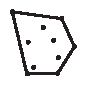
\includegraphics[width=\textwidth]{content/geometry/ConvexHull}
\vspace{-6mm}
\end{minipage}
 * Time: O(n \log n)
 * Status: stress-tested, tested with kattis:convexhull
*/

7d 7d #include "Point.h"

2c 2c typedef Point<ll> P;
b2 f1 vector<P> convexHull(vector<P> pts) {
4a f7 	if (sz(pts) <= 1) return pts;
55 3c 	sort(all(pts));
b9 ab 	vector<P> h(sz(pts)+1);
98 57 	int s = 0, t = 0;
0f 62 	for (int it = 2; it--; s = --t, reverse(all(pts)))
45 4e 		for (P p : pts) {
f3 3d 			while (t >= s + 2 && h[t-2].cross(h[t-1], p) <= 0) t--;
9e f3 			h[t++] = p;
dc cb 		}
dc 03 	return {h.begin(), h.begin() + t - (t == 2 && h[0] == h[1])};
ec cb }
\end{lstlisting}

\subsection{DelaunayTriangulation.cpp}
\begin{lstlisting}
Hash: 3d8be0
/**
 * Author: Mattias de Zalenski
 * Date: Unknown
 * Source: Geometry in C
 * Description: Computes the Delaunay triangulation of a set of points.
 *  Each circumcircle contains none of the input points.
 *  If any three points are collinear or any four are on the same circle, behavior is undefined.
 * Time: O(n^2)
 * Status: stress-tested
 */

7d 7d #include "Point.h"
e1 ad #include "3dHull.h"

6b 6a template<class P, class F>
f2 ff void delaunay(vector<P>& ps, F trifun) {
04 00 	if (sz(ps) == 3) { int d = (ps[0].cross(ps[1], ps[2]) < 0);
40 9a 		trifun(0,1+d,2-d); }
af 56 	vector<P3> p3;
8d 82 	for (P p : ps) p3.emplace_back(p.x, p.y, p.dist2());
73 08 	if (sz(ps) > 3) for(auto t:hull3d(p3)) if ((p3[t.b]-p3[t.a]).
b3 56 			cross(p3[t.c]-p3[t.a]).dot(P3(0,0,1)) < 0)
f0 15 		trifun(t.a, t.c, t.b);
3d cb }
\end{lstlisting}

\subsection{DistancePointTo.cpp}
\begin{lstlisting}
Hash: f203ff
/**
 * Author: Naim
 * Date: 2020-03-24
 * License: CC0
 * Source:
 * Description: Distance Point to things
 * Status: tested (maybe need stronger cases (??))
 */
7d 7d #include "Point.h"

d6 62 typedef Point<double> P;
1b bf const double EPS = 1e-9;
78 27 P projectPointLine(P a,P b,P p){
      	// to = M.(P-B)/(M.M);
c9 f7 	return a + (b-a)*((b-a).dot(p-a))/((b-a).dot(b-a));
1f cb }
f3 30 double distPointLine(P p,P a,P b){
76 fa 	return (p-projectPointLine(a,b,p)).dist();
13 cb }
42 5e double distPointRay(P p,P a,P b){
cf 9f 	P B = a,M = b-a;
      	// Line on the form L(t) = B + Mt ,t >=0;
a8 5b 	double to = M.dot(p - B)/M.dot(M);
      	
37 c2 	if(to<=EPS){
7b 88 		return (B-p).dist();
2c cb 	}
6d ea 	return (p-(B+M*to)).dist();
dc cb }

c8 5d double distPointSegment(P p,P a,P b){
d4 5d 	if(a==b)return (a-p).dist();
d6 9f 	P B = a,M=b-a;
87 5b 	double to = M.dot(p-B)/M.dot(M);
84 c2 	if(to<=EPS){// before 'a'
42 ac 		return (p-B).dist();
8c 11 	}else if(to>=1.0+EPS){//after 'b'; 
19 a4 		return (p-(B+M)).dist();
45 9d 	}else{// projection
05 ea 		return (p-(B+M*to)).dist();
16 cb 	}
      	// can use to project Point in segment
3f cb }

21 c2 pair<P,P> generatePoint(double a,double b,double c){
        // given a Line return two points to use in above functions
7c a3 	if(b==0){
a7 4c 		return make_pair(P(-1.0*c/a,0),P(-1.0*c/a,1));
21 cb 	}
8d 5e 	return make_pair(P(0,-1.0*c/b),P(1,1.0*(-a-c)/b));
f2 cb }
\end{lstlisting}

\subsection{DistPointInCircle.cpp}
\begin{lstlisting}
Hash: fdafeb
/**
 * Author: Naim
 * Date: 2020-03-30
 * Source:Math
 * Description:
 * dados a e b no circulo acha a distancia deles;
 * Centro eh C e raio R;
 * Usa Lei dos Cossenos Para calcular o angulo
 * Assume que a e b estao no circulo
 * Status: tested 
 */
 
7d 7d  #include "Point.h"
d6 62  typedef Point<double> P;
 
c6 c4  double distCircle(P a,P b,P C,double R){
      
ba 97     if((a-b).dist()<EPS)return (a-b).dist();
a4 2f     double d = (a-b).dist();
b1 3c     double ang = acos((d*d - 2.0*R*R)/(-2.0*R*R));
89 12     if(ang<0)ang+=2*PI;
          
52 13     return R*ang;
fd cb }
\end{lstlisting}

\subsection{DynamicUpperHull.cpp}
\begin{lstlisting}
Hash: 1b60eb
/*
  * Roubado do Ffao
  * Status: tested
*/
cd cd const ll is_query = -(1LL<<62);

dc 72 struct Line{
81 99  ll m,b;
c6 bf  mutable function<const Line*()> succ;
3f d9  bool operator <(const Line &rhs)const{
c1 d1     if(rhs.b!=is_query){
52 9e       if(m!=rhs.m)return m < rhs.m;
96 b3       return b > rhs.b;
b7 cb     }
99 3d     const Line* s = succ();
d9 de     if(!s)return 0;
73 1c     ll x = rhs.m;
56 ba     return b - s->b < (s->m - m)*x;
db cb  }
56 21 };


fa a2 struct DynamicHull : public multiset<Line>{ // upper hull for maximum
      
57 42   bool bad(iterator y){
21 e4     auto z = next(y);
91 1b     if(y==begin()){
b6 64       if(z==end())return 0;
cf 47       return y->m < z->m && y->b < z->b;
00 cb     }
      
c4 a9     auto x = prev(y);
69 18     if(z==end())return y->m < x->m && y->b < x->b;
32 ae     return (x->b - y->b)*(z->m - y->m) > (y->b - z->b)*(y->m - x->m);
be cb   }
      
b7 c4   void insert_line(ll m,ll b){
0d eb     auto y = insert({m,b});
3a b2     y->succ = [=]{
86 7f       return next(y)==end() ? 0 : &*next(y);
70 21     };
c8 86     if(bad(y)){erase(y);return;}
42 da     while(next(y)!=end() && bad(next(y)))erase(next(y));
fb c7     while(y!=begin() && bad(prev(y)))erase(prev(y));
f8 cb   }
bd 30   ll eval(ll x){
1e 3a     auto l = *lower_bound((Line){x,is_query});
b8 c7     return l.m*x + l.b;
ab cb   }
      
1b 21 };
\end{lstlisting}

\subsection{FastDelaunay.cpp}
\begin{lstlisting}
Hash: e8d11f
/**
 * Author: Philippe Legault
 * Date: 2016
 * License: MIT
 * Description: Fast Delaunay triangulation.
 * Each circumcircle contains none of the input points.
 * There must be no duplicate points.
 * If all points are on a line, no triangles will be returned.
 * Should work for doubles as well, though there may be precision issues in 'circ'.
 * Returns triangles in order \{t[0][0], t[0][1], t[0][2], t[1][0], \dots\}, all counter-clockwise.
 * Time: O(n \log n)
 * Status: stress-tested
 */

7d 7d #include "Point.h"

2c 2c typedef Point<ll> P;
05 80 typedef struct Quad* Q;
40 44 typedef __int128_t lll; // (can be ll if coords are < 2e4)
5c 59 P arb(LLONG_MAX,LLONG_MAX); // not equal to any other point

47 07 struct Quad {
c6 46 	Q rot, o; P p = arb; bool mark;
2b b3 	P& F() { return r()->p; }
68 23 	Q& r() { return rot->rot; }
0e f4 	Q prev() { return rot->o->rot; }
3e 57 	Q next() { return r()->prev(); }
76 97 } *H;

73 d1 bool circ(P p, P a, P b, P c) { // is p in the circumcircle?
a2 4b 	lll p2 = p.dist2(), A = a.dist2()-p2,
1f ff 	    B = b.dist2()-p2, C = c.dist2()-p2;
21 59 	return p.cross(a,b)*C + p.cross(b,c)*A + p.cross(c,a)*B > 0;
a0 cb }
83 00 Q makeEdge(P orig, P dest) {
3d bd 	Q r = H ? H : new Quad{new Quad{new Quad{new Quad{0}}}};
89 51 	H = r->o; r->r()->r() = r;
36 2c 	rep(i,0,4) r = r->rot, r->p = arb, r->o = i & 1 ? r : r->r();
eb ed 	r->p = orig; r->F() = dest;
c1 4c 	return r;
a5 cb }
1c d8 void splice(Q a, Q b) {
4a 68 	swap(a->o->rot->o, b->o->rot->o); swap(a->o, b->o);
24 cb }
f8 e9 Q connect(Q a, Q b) {
ac fc 	Q q = makeEdge(a->F(), b->p);
41 6e 	splice(q, a->next());
ad 64 	splice(q->r(), b);
1d be 	return q;
2f cb }

87 19 pair<Q,Q> rec(const vector<P>& s) {
ff e6 	if (sz(s) <= 3) {
2c 4a 		Q a = makeEdge(s[0], s[1]), b = makeEdge(s[1], s.back());
e3 2b 		if (sz(s) == 2) return { a, a->r() };
b9 19 		splice(a->r(), b);
f9 5f 		auto side = s[0].cross(s[1], s[2]);
43 b9 		Q c = side ? connect(b, a) : 0;
64 3d 		return {side < 0 ? c->r() : a, side < 0 ? c : b->r() };
32 cb 	}
      
6d 5e #define H(e) e->F(), e->p
bc c9 #define valid(e) (e->F().cross(H(base)) > 0)
93 a3 	Q A, B, ra, rb;
59 f5 	int half = sz(s) / 2;
91 39 	tie(ra, A) = rec({all(s) - half});
8f d9 	tie(B, rb) = rec({sz(s) - half + all(s)});
95 f8 	while ((B->p.cross(H(A)) < 0 && (A = A->next())) ||
63 b0 	       (A->p.cross(H(B)) > 0 && (B = B->r()->o)));
f6 76 	Q base = connect(B->r(), A);
fa 87 	if (A->p == ra->p) ra = base->r();
31 b5 	if (B->p == rb->p) rb = base;
      
f1 3e #define DEL(e, init, dir) Q e = init->dir; if (valid(e)) \
cf f0 		while (circ(e->dir->F(), H(base), e->F())) { \
72 93 			Q t = e->dir; \
29 6d 			splice(e, e->prev()); \
bf 16 			splice(e->r(), e->r()->prev()); \
48 d4 			e->o = H; H = e; e = t; \
97 cb 		}
b0 1d 	for (;;) {
2c ea 		DEL(LC, base->r(), o);  DEL(RC, base, prev());
e9 6f 		if (!valid(LC) && !valid(RC)) break;
71 e0 		if (!valid(LC) || (valid(RC) && circ(H(RC), H(LC))))
94 b7 			base = connect(RC, base->r());
0d 29 		else
6b 27 			base = connect(base->r(), LC->r());
ac cb 	}
40 34 	return { ra, rb };
54 cb }

7f da vector<P> triangulate(vector<P> pts) {
ab af 	sort(all(pts));  assert(unique(all(pts)) == pts.end());
5e e0 	if (sz(pts) < 2) return {};
06 23 	Q e = rec(pts).first;
0b 50 	vector<Q> q = {e};
c5 6c 	int qi = 0;
ac 7a 	while (e->o->F().cross(e->F(), e->p) < 0) e = e->o;
12 80 #define ADD { Q c = e; do { c->mark = 1; pts.push_back(c->p); \
b5 0b 	q.push_back(c->r()); c = c->next(); } while (c != e); }
03 9d 	ADD; pts.clear();
19 b5 	while (qi < sz(q)) if (!(e = q[qi++])->mark) ADD;
54 a4 	return pts;
e8 cb }
\end{lstlisting}

\subsection{HalfPlaneIntersec.cpp}
\begin{lstlisting}
Hash: fd24b4
/**
 * Source: Lib do Gabriel Pessoa
 * Status: Testado no "big brother" apenas...
**/
7d 7d #include "Point.h"
b1 c4 #include "lineIntersection.h"

6c 62 typedef Point<double> P;
52 32 typedef Point<double> PT;

7a f2 struct L {
8e 38     PT a, b;
b8 fe     double ang;
19 03     L(){}
14 1a     L(PT a, PT b) : a(a), b(b) {}
6b 21 };

ef b2 double angle (L la) { return atan2(-(la.a.y - la.b.y), la.b.x - la.a.x); }

f0 bc const double inf = 1e100, eps = 1e-9;
75 6c const double PI = acos(-1.0L);

b3 ec int cmp (double a, double b = 0) {
96 b7   if (abs(a-b) < eps) return 0;
9c cf   return (a < b) ? -1 : +1;
65 cb }

d2 58 bool comp (L la, L lb) {       
02 fc     if (cmp(la.ang, lb.ang) == 0) return (lb.b - lb.a).cross(la.b - lb.a) > eps;
f5 f8     return cmp(la.ang,lb.ang) < 0;
8e cb }


5c ce pair<int, PT> lineInter(L la,L lb){
7e 50   return lineInter(la.a,la.b,lb.a,lb.b);
8b cb }

46 28 bool check (L la, L lb, L lc) {
3f b0     PT p = lineInter(lb, lc).ss;
ba f3     double det = (la.b - la.a).cross(p - la.a);
e3 b2     return cmp(det) < 0;
b4 cb }


fd 2c const int N = 500100;
fe af int dq[2*N]; // pode substituir por um deque normal
44 09 int idl,idr; // idr++ -> push_back, idr-- (popback), idl++(popfront)

// pi->pj - esquerda
// NAO FUNCIONA NEM FOI TESTADO SE NAO RETORNAR ALGO CONVEXO

cc 7f vector<PT> hpi (vector<L> line) { // salvar (i, j) CCW, (j, i) CW
f8 3a     rep(i,0,sz(line))line[i].ang = angle(line[i]);
7d 93     sort(line.begin(), line.end(), comp);
9d 88     vector<L> pl(1, line[0]);
ed 95     for (int i = 0; i < (int)line.size(); ++i) if (cmp(angle(line[i]), angle(pl.back())) != 0) pl.push_back(line[i]);
b5 5e     idl = N,idr = N;
27 35     dq[idr++]=(0);
d0 cb     dq[idr++]=(1);
00 70     for (int i = 2; i < (int)pl.size(); ++i) {
00 96         while (idr - idl > 1 && check(pl[i], pl[dq[idr-1]], pl[dq[idr - 2]])) idr--;
c5 74         while (idr - idl > 1 && check(pl[i], pl[dq[idl]], pl[dq[idl+1]])) idl++;
2f 08         dq[idr++]=i;
34 cb     }
cc 4a     while (idr - idl > 1 && check(pl[dq[idl]], pl[dq[idr-1]], pl[dq[idr - 2]])) idr--;
05 2d     while (idr - idl > 1 && check(pl[dq[idr-1]], pl[dq[idl]], pl[dq[idl + 1]])) idl++;
47 81     vector<PT> res;
a7 93     for (int i = 0; i < idr - idl; ++i){
51 95       int nxt = (idl + i + 1 == idr ? idl : idl + i+1);
9b 56       auto IT = lineInter(pl[dq[idl + i]], pl[dq[nxt]]);
8e e0       if(IT.ff!=1){ // Nao retorna uma area convexa
49 ae         res.clear();
77 b5         return res;
32 cb       }
4e 94       res.pb(IT.ss);
2b cb     }
3b b5     return res;
fd cb }
\end{lstlisting}

\subsection{HalfPlaneMIT.cpp}
\begin{lstlisting}
Hash: 0da892
7d 7d template<class P>
bd 19 int lineIntersection(const P& s1, const P& e1, const P& s2,
cb 4d 		const P& e2, P& r) {
5f fd 	if ((e1-s1).cross(e2-s2)) { //if not parallell
ea a4 		r = s2-(e2-s2)*(e1-s1).cross(s2-s1)/(e1-s1).cross(e2-s2);
5c 6a 		return 1;
62 ce 	} else
79 df 		return -((e1-s1).cross(s2-s1)==0 || s2==e2);
aa cb }
 
 
50 36 #define eps 1e-8
6f 62 typedef Point<double> P;
 
87 72 struct Line {
6d e4 	P P1, P2;
      	// Right hand side of the ray P1 -> P2
30 54 	explicit Line(P a = P(), P b = P()) : P1(a), P2(b) {};
a1 4c 	P intpo(Line y) {
35 25 		P r;
18 a5 		assert(lineIntersection(P1, P2, y.P1, y.P2, r) == 1);
c7 4c 		return r;
b1 cb 	}
2f db 	P dir() {
d6 c6 		return P2 - P1;
da cb 	}
9d ad 	bool contains(P x) {
39 44 		return (P2 - P1).cross(x - P1) < eps;
ee cb 	}
b8 2c 	bool out(P x) {
5c 0b 		return !contains(x);
d3 cb 	}
f1 21 }; 
 
1c 4f template<class T>
a1 78 bool mycmp(Point<T> a, Point<T> b) {
      	// return atan2(a.y, a.x) < atan2(b.y, b.x);
57 2a 	if (a.x * b.x < 0)	return a.x < 0;
69 7a 	if (abs(a.x) < eps) {
11 13 		if (abs(b.x) < eps) 	return a.y > 0 && b.y < 0;
b3 50 		if (b.x < 0)	return a.y > 0;
a1 19 		if (b.x > 0)	return true;
b7 cb 	}
07 13 	if (abs(b.x) < eps) {
fc 04 		if (a.x < 0)	return b.y < 0;
e4 b8 		if (a.x > 0)	return false;
bc cb 	}
63 c3 	return a.cross(b) > 0;
41 cb }
 
81 a3 bool cmp(Line a, Line b) {
6f 9c 	return mycmp(a.dir(), b.dir());
8c cb }
 
20 10 double Intersection_Area(vector <Line> b) {
4f e2 	sort(b.begin(), b.end(), cmp);
45 4c 	int n = b.size();
08 17 	int q = 1, h = 0, i;
04 b3 	vector <Line> c(b.size() + 10);
da 3f 	for (i = 0; i < n; i++) {
2f b9 		while (q < h && b[i].out(c[h].intpo(c[h - 1])))	h--;
d3 d0 		while (q < h && b[i].out(c[q].intpo(c[q + 1])))	q++;
fa 35 		c[++h] = b[i];
db 1c 		if (q < h && abs(c[h].dir().cross(c[h - 1].dir())) < eps) {
ff df 			h--;
ee b6 			if (b[i].out(c[h].P1))	c[h] = b[i];
08 cb 		}
62 cb 	}
6e 6f 	while (q < h - 1 && c[q].out(c[h].intpo(c[h - 1])))	h--;
23 b1 	while (q < h - 1 && c[h].out(c[q].intpo(c[q + 1])))	q++;
      	// Intersection is empty. This is sometimes different from the case when
      	// the intersection area is 0. 
73 2a 	if (h - q <= 1)	return -1;
76 27 	c[h + 1] = c[q];
3d c2 	vector <P> s;
b8 33 	for (i = q; i <= h; i++)	s.push_back(c[i].intpo(c[i + 1]));
00 6e 	s.push_back(s[0]);
9d e9 	double ans = 0;
c8 5d 	for (i = 0; i < (int) s.size() - 1; i++)	ans += s[i].cross(s[i + 1]);
9a 48 	return ans / 2;
d0 cb }
 
f7 1a int n;
16 28 P a[61000];
 
7f ed bool ok(int x) {
c6 40 	vector <Line> b;
ae 83 	for (int i = 0; i < n; i++)
eb 55 		b.push_back(Line(a[i], a[(i + x) % n]));
2e bb 	if (Intersection_Area(b) > eps)
57 8a 		return true;
14 29 	else
45 d1 		return false;
0d cb }
 
\end{lstlisting}

\subsection{HullLine.cpp}
\begin{lstlisting}
Hash: 33a260
/**
 * Author: Oleksandr Bacherikov, chilli
 * Date: 2019-05-07
 * License: Boost Software License
 * Description: Line-convex polygon intersection. The polygon must be ccw and have no colinear points.
 * lineHull(line, poly) returns a pair describing the intersection of a line with the polygon:
 *  \begin{itemize*}
 *    \item $(-1, -1)$ if no collision,
 *    \item $(i, -1)$ if touching the corner $i$,
 *    \item $(i, i)$ if along side $(i, i+1)$,
 *    \item $(i, j)$ if crossing sides $(i, i+1)$ and $(j, j+1)$.
 *  \end{itemize*}
 *  In the last case, if a corner $i$ is crossed, this is treated as happening on side $(i, i+1)$.
 *  The points are returned in the same order as the line hits the polygon.
 * \texttt{extrVertex} returns the point of a hull with the max projection onto a line.
 * Status: stress-tested
 * Time: O(N + Q \log n)
 */

7d 7d #include "Point.h"

de 53 #define cmp(i,j) sgn(dir.perp().cross(poly[(i)%n]-poly[(j)%n]))
52 f8 #define extr(i) cmp(i + 1, i) >= 0 && cmp(i, i - 1 + n) < 0
cb e7 template <class P> int extrVertex(vector<P>& poly, P dir) {
a2 74 	int n = sz(poly), lo = 0, hi = n;
df fd 	if (extr(0)) return 0;
a9 3d 	while (lo + 1 < hi) {
47 59 		int m = (lo + hi) / 2;
64 85 		if (extr(m)) return m;
62 c0 		int ls = cmp(lo + 1, lo), ms = cmp(m + 1, m);
69 f4 		(ls < ms || (ls == ms && ls == cmp(lo, m)) ? hi : lo) = m;
cd cb 	}
28 25 	return lo;
24 cb }

78 8e #define cmpL(i) sgn(a.cross(poly[i], b))
cd 7d template <class P>
f6 38 array<int, 2> lineHull(P a, P b, vector<P> poly) {
ee 40 	int endA = extrVertex(poly, (a - b).perp());
70 76 	int endB = extrVertex(poly, (b - a).perp());
02 1a 	if (cmpL(endA) < 0 || cmpL(endB) > 0)
be 42 		return {-1, -1};
5b 64 	array<int, 2> res;
3e f4 	rep(i,0,2) {
ce 23 		int lo = endB, hi = endA, n = sz(poly);
6d c2 		while ((lo + 1) % n != hi) {
9c 57 			int m = ((lo + hi + (lo < hi ? 0 : n)) / 2) % n;
e7 7f 			(cmpL(m) == cmpL(endB) ? lo : hi) = m;
21 cb 		}
2a 7d 		res[i] = (lo + !cmpL(hi)) % n;
a8 35 		swap(endA, endB);
55 cb 	}
fc e0 	if (res[0] == res[1]) return {res[0], -1};
ea 3d 	if (!cmpL(res[0]) && !cmpL(res[1]))
d7 95 		switch ((res[0] - res[1] + sz(poly) + 1) % sz(poly)) {
b6 3f 			case 0: return {res[0], res[0]};
e3 22 			case 2: return {res[1], res[1]};
42 cb 		}
0d b5 	return res;
33 cb }
\end{lstlisting}

\subsection{InversiveGeometry.cpp}
\begin{lstlisting}
Hash: 0fac2a
/**
 * Author: Matheus Leal
 * Date: 31/01/2021
 * Description:
   IMPORTANTE: Um bom raio para evitar overflow ou precisao eh sqrt(dmin * dmax)
   
	 Dado uma circumferencia C de centro O e raio R e um ponto P, retornar o inverso de P utilizando C como referencia.
   OP*OP' = r^2
   O inverso de um ponto que toca a circunferencia nao eh alterado
   se O = P -> Inverso eh infinito, entao temos uma circunferencia centrada em infinito (uma reta), onde a parte interna eh um semiplano
   que nao possui o centro O dentro
 * Status: tested with 40th Petrozavodsk camp - day2 F. Friendship circles
 * Time: O(1)
*/

7d 7d #include "Point.h"

//Modificar
ca 5d typedef Point<long double> P;

32 fa long double dist(P a, P b){
f1 c3 	return sqrt((a.x-b.x)*(a.x-b.x) + (a.y - b.y)*(a.y-b.y));
9c cb }

//NUNCA PERGUNTAR O INVERSO DO CENTRO
bd 92 P InversiveFromCircle(P o, long double r, P p) {
f0 c6 	assert(!(o == p));
55 93 	long double OP = dist(o, p);
fc 20 	long double OP1 = (r*r)/OP;
ff eb 	long double c = OP1/OP;
3d 8c 	P q = P(c*(p.x - o.x) + o.x, c*(p.y - o.y) + o.y);
d7 be 	return q; 
0f cb }
\end{lstlisting}

\subsection{LargestQuadArea.cpp}
\begin{lstlisting}
Hash: 2f48b4
/*
 * Given a Convex Hull, find the area of the biggest Quadrileteral.
 * If the Hull has 3 points, we brute the 4th one ( v has the hull and v2 the original points )
 * O(N**2)
 * Status: Tested
 * Note: Better to use Minkowski (31ms vs 1800ms) , only added because of the two pointers technique 
*/

e8 e8 ll largestAreaQuad(){
      	
79 35 		if(v.size()<3){
5d bb 			return 0;
03 cb 		}
      		
      		
71 49 		if(v.size()==3){
85 f0 			ll best = 0;
04 ba 			int n = v2.size();
07 60 			for(int i=0;i<n;i++){
13 fe 				if(v2[i]==v[0] || v2[i]==v[1] || v2[i]==v[2])continue;// only if doesnt have equal points! If it does, use ids
bf 4c 				ll tudo = polygonArea2(v);
37 51 				ll op1 = abs(v2[i].cross(v[0],v[1]));
c1 bd 				ll op2 = abs(v2[i].cross(v[0],v[2]));
99 97 				ll op3 = abs(v2[i].cross(v[1],v[2]));
8b cf 				best = max(best,tudo - min({op1,op2,op3}));
85 cb 			}
      
2b f2 			return best;
ae cb 		}
      		
98 d6 		 n = v.size();
06 f0 		ll best = 0;	
4f 60 		for(int i=0;i<n;i++){
      
18 b4 			int j = (i+2)%n;
37 f6 			int l = (i+1)%n;
ac b6 			int r = (i+3)%n;
88 26 			auto next = [&](int j){
41 85 				if(j+1>=n)return j+1-n;
62 75 				return j+1;
ab 21 			};
0b e0 			auto area = [&](int i,int j,int k){
0f 7e 				return abs(v[k].cross(v[i],v[j]));
b7 21 			};
83 02 			while(i!=j){
03 dc 				while(next(l)!=j && area(i,j,next(l)) >= area(i,j,l)){
35 83 					l = next(l);
62 cb 				}
      				
d3 ec 				while(next(r)!=i && area(i,j,next(r))>=area(i,j,r)){
2e 0b 					r =	next(r);
52 cb 				}
c4 85 				best = max(best,area(i,j,l) + area(i,j,r));
71 6c 				j=next(j);
dd cb 			}
      
      
b8 cb 		}
      
d7 f2 		return best;
2f cb }
\end{lstlisting}

\subsection{LineDistance.cpp}
\begin{lstlisting}
Hash: d1d032
/**
 * Author: Ulf Lundstrom
 * Date: 2009-03-21
 * License: CC0
 * Source: Basic math
 * Description:\\
\begin{minipage}{75mm}
Returns the signed distance between point p and the line containing points a and b. Positive value on left side and negative on right as seen from a towards b. a==b gives nan. P is supposed to be Point<T> or Point3D<T> where T is e.g. double or long long. It uses products in intermediate steps so watch out for overflow if using int or long long. Using Point3D will always give a non-negative distance. For Point3D, call .dist on the result of the cross product.
\end{minipage}
\begin{minipage}{15mm}
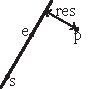
\includegraphics[width=\textwidth]{content/geometry/lineDistance}
\end{minipage}
 * Status: tested
 */

7d 7d #include "Point.h"

07 7d template<class P>
3d 2f double lineDist(const P& a, const P& b, const P& p) {
57 e0 	return (double)(b-a).cross(p-a)/(b-a).dist();
d1 cb }
\end{lstlisting}

\subsection{LineIntersection.cpp}
\begin{lstlisting}
Hash: ae219b
/**
 * Author: Victor Lecomte, chilli
 * Date: 2019-05-05
 * License: CC0
 * Description:\\
\begin{minipage}{75mm}
If a unique intersection point of the lines going through s1,e1 and s2,e2 exists \{1, point\} is returned.
If no intersection point exists \{0, (0,0)\} is returned and if infinitely many exists \{-1, (0,0)\} is returned.
The wrong position will be returned if P is Point<ll> and the intersection point does not have integer coordinates.
Products of three coordinates are used in intermediate steps so watch out for overflow if using int or ll.
\end{minipage}
\begin{minipage}{15mm}
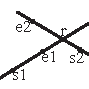
\includegraphics[width=\textwidth]{content/geometry/lineIntersection}
\end{minipage}
 * Status: stress-tested, and tested through half-plane tests
 * Usage:
 * 	auto res = lineInter(s1,e1,s2,e2);
 * 	if (res.first == 1)
 * 		cout << "intersection point at " << res.second << endl;
 */

7d 7d #include "Point.h"

07 7d template<class P>
94 0b pair<int, P> lineInter(P s1, P e1, P s2, P e2) {
f9 14 	auto d = (e1 - s1).cross(e2 - s2);
08 8c 	if (d == 0) // if parallel
8f d9 		return {-(s1.cross(e1, s2) == 0), P(0, 0)};
1d f6 	auto p = s2.cross(e1, e2), q = s2.cross(e2, s1);
b9 9b 	return {1, (s1 * p + e1 * q) / d};
ae cb }
\end{lstlisting}

\subsection{LineProjectionReflection.cpp}
\begin{lstlisting}
Hash: c08b13
/**
 * Author: Victor Lecomte, chilli
 * Date: 2019-10-29
 * License: CC0
 * Description: Projects point p onto line ab. Set refl=true to get reflection
 * of point p across line ab insted. The wrong point will be returned if P is
 * an integer point and the desired point doesn't have integer coordinates.
 * Products of three coordinates are used in intermediate steps so watch out
 * for overflow.
 * Status: stress-tested
  !!! caso de overflow pode usar a + (b-a) * dot(b-a,c-a)/dot(b-a,b-a) para pegar a projecao de c em a-b;
  Lembrando que isso vem de L(t) = B + M*t, to = M.(P-B)/(M.M) . 
  // para mudar para ray-> to>=0 , para segmento to =[0,1];
 */

7d 7d #include "Point.h"

07 7d template<class P>
45 98 P lineProj(P a, P b, P p, bool refl=false) {
17 de 	P v = b - a;
4f 3f 	return p - v.perp()*(1+refl)*v.cross(p-a)/v.dist2();
c0 cb }
\end{lstlisting}

\subsection{ManhattanMST.cpp}
\begin{lstlisting}
Hash: c264e8
/**
 * Author: chilli, Takanori MAEHARA
 * Date: 2019-11-02
 * License: CC0
 * Description: Given N points, returns up to 4*N edges, which are guaranteed
 * to contain a minimum spanning tree for the graph with edge weights w(p, q) =
 * |p.x - q.x| + |p.y - q.y|. Edges are in the form (distance, src, dst). Use a
 * standard MST algorithm on the result to find the final MST.
 * Time: O(N \log N)
 * Status: Stress-tested
 */
7d 7d #include "Point.h"

d6 bb typedef Point<int> P;
2b ea vector<array<int, 3>> manhattanMST(vector<P> ps) {
ba 85 	vi id(sz(ps));
44 27 	iota(all(id), 0);
1c 8c 	vector<array<int, 3>> edges;
46 8d 	rep(k,0,4) {
36 1d 		sort(all(id), [&](int i, int j) {
22 0d 		     return (ps[i]-ps[j]).x < (ps[j]-ps[i]).y;});
c3 70 		map<int, int> sweep;
13 1e 		for (int i : id) {
c1 84 			for (auto it = sweep.lower_bound(-ps[i].y);
33 90 				        it != sweep.end(); sweep.erase(it++)) {
21 61 				int j = it->second;
30 6f 				P d = ps[i] - ps[j];
e2 d1 				if (d.y > d.x) break;
49 53 				edges.push_back({d.y + d.x, i, j});
65 cb 			}
6a 92 			sweep[-ps[i].y] = i;
8b cb 		}
4a 4e 		for (P& p : ps) if (k & 1) p.x = -p.x; else swap(p.x, p.y);
29 cb 	}
9f da 	return edges;
c2 cb }
\end{lstlisting}

\subsection{Minimalenclosingcircle.cpp}
\begin{lstlisting}
Hash: 0b9ff5
/**
 * Author: Andrew He, chilli
 * Date: 2019-05-07
 * License: CC0
 * Source: folklore
 * Description: Computes the minimum circle that encloses a set of points.
 * Time: expected O(n)
 * Status: stress-tested
 */

a2 a2 #include "circumcircle.h"

e2 a2 pair<P, double> mec(vector<P> ps) {
0a 4d 	shuffle(all(ps), mt19937(time(0)));
b5 f6 	P o = ps[0];
28 32 	double r = 0, EPS = 1 + 1e-8;
ca 2b 	rep(i,0,sz(ps)) if ((o - ps[i]).dist() > r * EPS) {
15 5c 		o = ps[i], r = 0;
db 4d 		rep(j,0,i) if ((o - ps[j]).dist() > r * EPS) {
cb a3 			o = (ps[i] + ps[j]) / 2;
55 6f 			r = (o - ps[i]).dist();
ba 10 			rep(k,0,j) if ((o - ps[k]).dist() > r * EPS) {
3c fa 				o = ccCenter(ps[i], ps[j], ps[k]);
1c 6f 				r = (o - ps[i]).dist();
37 cb 			}
40 cb 		}
10 cb 	}
c2 64 	return {o, r};
0b cb }
\end{lstlisting}

\subsection{Minkowski.cpp}
\begin{lstlisting}
Hash: ebec95
/**
 * Author: Tiago Domingos
 * Date: 14/02/2020
 * Description:
	Given two convex polygons (ccw, sorted by polar angle by the min lex.)
	return the minkowski sum of the two of then (if a is an vector in A, b in B, A^B contains (a+b))
	It may contain collinear points, but can easily be treated while making the minkowski sum
 * Status: multi-tested 
 * Time: O(n + m)
*/

2c 2c typedef Point<ll> P;
9a f8 vector<P> minkowski(const vector<P> &A ,const vector<P> &B){
22 2f 	vector<P> e;
1b 7d 	e.push_back(A[0] + B[0]);
54 69 	int i = 0 , j = 0 ;
b0 f9 	auto comp = [&](P a , P b){
d7 ab 		int hp1 = (a.x < 0 || (a.x == 0 && a.y < 0)) , hp2 = (b.x < 0 || (b.x == 0 && b.y < 0));
d0 07 		if(hp1 != hp2) return hp1 < hp2;
fb 48 		if(a.cross(b) != 0){
fe c3 			return a.cross(b)  > 0;
33 cb 		}
16 ba 		return a.dist2() < b.dist2();
b6 21 	};
15 7c 	while(i != sz(A) || j != sz(B)){
08 f4 		P a = A[(i+1)%sz(A)] - A[i] , b = B[(j+1)%sz(B)] - B[j];
6a 56 		if(i == sz(A)) e.push_back(e.back() + b) , j++;
4c 20 		else if(j == sz(B)) e.push_back(e.back() + a), i++;
f3 4e 		else{
2a 30 			if(comp(a,b)) e.push_back(e.back() + a) , i++;
b6 0e 			else e.push_back(e.back() + b) , j ++;
01 cb 		}
0f cb 	}
a2 d6 	e.pop_back();
d1 6b 	return e;
4a cb }
// warning : e contains colinear points, you can easily remove in the merge step 


// cp algo:
22 92 void reorder_polygon(vector<pt> & P){
3d 65     size_t pos = 0;
a4 81     for(size_t i = 1; i < P.size(); i++){
e4 0e         if(P[i].y < P[pos].y || (P[i].y == P[pos].y && P[i].x < P[pos].x))
17 e4             pos = i;
67 cb     }
45 98     rotate(P.begin(), P.begin() + pos, P.end());
96 cb }

e6 e4 vector<pt> minkowski(vector<pt> P, vector<pt> Q){
          // the first vertex must be the lowest
d8 15     reorder_polygon(P);
92 fa     reorder_polygon(Q);
          // we must ensure cyclic indexing
0b 64     P.push_back(P[0]);
55 6e     P.push_back(P[1]);
82 40     Q.push_back(Q[0]);
7e d1     Q.push_back(Q[1]);
          // main part
51 ed     vector<pt> result;
a8 a0     size_t i = 0, j = 0;
12 65     while(i < P.size() - 2 || j < Q.size() - 2){
ce d8         result.push_back(P[i] + Q[j]);
47 60         auto cross = (P[i + 1] - P[i]).cross(Q[j + 1] - Q[j]);
96 a7         if(cross >= 0)
76 c7             ++i;
a7 f2         if(cross <= 0)
9b 3c             ++j;
86 cb     }
da dc     return result;
eb cb }
\end{lstlisting}

\subsection{MultipleSegInter.cpp}
\begin{lstlisting}
Hash: 91148f
 * Finds a pair of intersecting segments or returns (-1,-1) if there is no pair
 * Each segment needs a unique id
 */
08 08  typedef long double ld;
67 b2  struct pt {
49 c1     ld x, y;
27 88     pt(ld x, ld y) : x(x), y(y) {}
34 21 };

e8 5a const ld EPS = 1e-12;

81 8b struct seg {
bf 73     pt p, q;
87 53     int id;
21 e0     seg(pt& x, pt& y, int& id) : p(x), q(y), id(id) {}
       
ef d6     ld get_y (ld x) const {
48 6a         if (abs (p.x - q.x) < EPS)  return p.y;
90 df         return p.y + (q.y - p.y) * (x - p.x) / (q.x - p.x);
1f cb     }
f4 21 };
 
 
ea cf inline bool intersect1d (ld l1, ld r1, ld l2, ld r2) {
a9 58     if (l1 > r1)  swap (l1, r1);
30 c4     if (l2 > r2)  swap (l2, r2);
8b 55     return max (l1, l2) <= min (r1, r2) + EPS;
b7 cb }
 
35 72 inline int vec (const pt & a, const pt & b, const pt & c) {
60 d7     ld s = (b.x - a.x) * (c.y - a.y) - (b.y - a.y) * (c.x - a.x);
63 40     return abs(s)<EPS ? 0 : s>0 ? +1 : -1;
f7 cb }
 
46 01 bool intersect (const seg & a, const seg & b) {
2f ff     return intersect1d (a.p.x, a.q.x, b.p.x, b.q.x)
e7 d1            && intersect1d (a.p.y, a.q.y, b.p.y, b.q.y)
f2 72            && vec (a.p, a.q, b.p) * vec (a.p, a.q, b.q) <= 0
4d 83            && vec (b.p, b.q, a.p) * vec (b.p, b.q, a.q) <= 0;
61 cb }
 
 
c8 4c bool operator< (const seg & a, const seg & b) {
9a 3b     ld x = max (min (a.p.x, a.q.x), min (b.p.x, b.q.x));
02 77     return a.get_y(x) < b.get_y(x) - EPS;
a5 cb }
 
 
a3 2c struct has_inter {
       
19 cc     struct event {
c4 e5         ld x;
4a b5         int tp, id;
       
58 7b         event() {}
       
4d 24         event(ld x, int tp, int id)
cf f1             : x(x), tp(tp), id(id) {}
       
66 73         bool operator<(const event &e) const {
d4 29             if (abs(x - e.x) > EPS) return x < e.x;
3c 18             return tp > e.tp;
db cb         }
30 21     };
       
91 92     set<seg> s;
2b bc     vector<set<seg>::iterator> where;
       
f5 96     inline set<seg>::iterator prev(set<seg>::iterator it) {
aa 68         return it == s.begin() ? s.end() : --it;
37 cb     }
       
86 e8     inline set<seg>::iterator next(set<seg>::iterator it) {
ad f1         return ++it;
74 cb     }
       
d5 33     pair<int, int> solve(const vector<seg> &a) {
6c 8e         int n = (int) a.size();
e6 c9         vector<event> e;
79 ba         for (int i = 0; i < n; ++i) {
be b4             e.push_back(event(min(a[i].p.x, a[i].q.x), +1, i));
36 c4             e.push_back(event(max(a[i].p.x, a[i].q.x), -1, i));
ec cb         }
ef af         sort(e.begin(), e.end());
       
d0 e6         s.clear();
d3 b1         where.resize(a.size());
61 22         for (size_t i = 0; i < e.size(); ++i) {
9d cf             int id = e[i].id;
95 9d             if (e[i].tp == +1) {
cf c3                 auto nxt = s.lower_bound(a[id]), prv = prev(nxt);
4c fb                 if (nxt != s.end() && intersect(*nxt, a[id]))
c0 0e                     return make_pair(nxt->id, id);
8f 69                 if (prv != s.end() && intersect(*prv, a[id]))
03 d4                     return make_pair(prv->id, id);
f6 84                 where[id] = s.insert(nxt, a[id]);
9c 9d             } else {
79 39                 if (where[id] == s.end()) continue;
7e d6                 auto nxt = next(where[id]), prv = prev(where[id]);
4f e7                 if (nxt != s.end() && prv != s.end() && intersect(*nxt, *prv))
2f 58                     return make_pair(prv->id, nxt->id);
e8 2c                 s.erase(where[id]);
c9 cb             }
21 cb         }
       
61 8a         return make_pair(-1, -1);
72 cb     }
91 21 };
\end{lstlisting}

\subsection{OnSegment.cpp}
\begin{lstlisting}
Hash: 5fde08
/**
 * Author: Victor Lecomte, chilli
 * Date: 2019-04-26
 * License: CC0
 * Description: Returns true iff p lies on the line segment from s to e.
 * Use \texttt{(segDist(s,e,p)<=epsilon)} instead when using Point<double>.
 * Status:
 */

7d 7d #include "Point.h"

a7 51 template<class P> bool onSegment(P s, P e, P p) {
59 5f 	return p.cross(s, e) == 0 && (s - p).dot(e - p) <= 0;
5f cb }
\end{lstlisting}

\subsection{Point.cpp}
\begin{lstlisting}
Hash: 47ec0a
/**
 * Description: Class to handle points in the plane.
 * 	T can be e.g. double or long long. (Avoid int.)
 * Status: Works fine, used a lot
 */

48 48 template <class T> int sgn(T x) { return (x > 0) - (x < 0); }
fc 4f template<class T>
74 f2 struct Point {
f7 ea 	typedef Point P;
fa 64 	T x, y;
55 ea 	explicit Point(T x=0, T y=0) : x(x), y(y) {}
1a 0d 	bool operator<(P p) const { return tie(x,y) < tie(p.x,p.y); }
3a ec 	bool operator==(P p) const { return tie(x,y)==tie(p.x,p.y); }
1d 27 	P operator+(P p) const { return P(x+p.x, y+p.y); }
18 40 	P operator-(P p) const { return P(x-p.x, y-p.y); }
26 e0 	P operator*(T d) const { return P(x*d, y*d); }
8c 0b 	P operator/(T d) const { return P(x/d, y/d); }
71 57 	T dot(P p) const { return x*p.x + y*p.y; }
7e 46 	T cross(P p) const { return x*p.y - y*p.x; }
52 b3 	T cross(P a, P b) const { return (a-*this).cross(b-*this); }
e7 f6 	T dist2() const { return x*x + y*y; }
03 18 	double dist() const { return sqrt((double)dist2()); }
      	// angle to x-axis in interval [-pi, pi]
cc 90 	double angle() const { return atan2(y, x); }
b0 d0 	P unit() const { return *this/dist(); } // makes dist()=1
e0 20 	P perp() const { return P(-y, x); } // rotates +90 degrees
c0 85 	P normal() const { return perp().unit(); }
      	// returns point rotated 'a' radians ccw around the origin
91 f2 	P rotate(double a) const {
e4 f5 		return P(x*cos(a)-y*sin(a),x*sin(a)+y*cos(a)); }
70 90 	friend ostream& operator<<(ostream& os, P p) {
0e 05 		return os << "(" << p.x << "," << p.y << ")"; }
47 21 };
\end{lstlisting}

\subsection{PointInsideHull.cpp}
\begin{lstlisting}
Hash: 1710a2
/**
 * Author: chilli
 * Date: 2019-05-17
 * License: CC0
 * Description: Determine whether a point t lies inside a convex hull (CCW
 * order, with no colinear points). Returns true if point lies within
 * the hull. If strict is true, points on the boundary aren't included.
 * !!! IF DOUBLE : Replace onSegment by sedDist <=EPS , and use sideOf(l[0],l[a],l[b],EPS) 
 * Usage:
 * Status: stress-tested
 * Time: O(\log N)
 */

7d 7d #include "Point.h"
7e 12 #include "sideOf.h"
d5 8f #include "OnSegment.h"

cc 2c typedef Point<ll> P;

aa 2d bool inHull(const vector<P>& l, P p, bool strict = true) {
20 d4 	int a = 1, b = sz(l) - 1, r = !strict;
1e 5c 	if (sz(l) < 3) return r && onSegment(l[0], l.back(), p);
09 6b 	if (sideOf(l[0], l[a], l[b]) > 0) swap(a, b);
bf 45 	if (sideOf(l[0], l[a], p) >= r || sideOf(l[0], l[b], p)<= -r)
2a d1 		return false;
d0 48 	while (abs(a - b) > 1) {
aa 4f 		int c = (a + b) / 2;
cc ac 		(sideOf(l[0], l[c], p) > 0 ? b : a) = c;
2e cb 	}
46 06 	return sgn(l[a].cross(l[b], p)) < r;
17 cb }
\end{lstlisting}

\subsection{PointInsidePolygon.cpp}
\begin{lstlisting}
Hash: 850cb2
/* Checks if a point is inside a Polygon, dont needs to be convex
 * Better usages with long long
 * Status: Weakly tested on ASC 1, problem F
*/

7d 7d #include "Point.h"
94 8f #include "OnSegment.h"


d8 ff bool above(P a,P p){
dc d3 	return p.y >= a.y;
de cb }

2b 7c bool crossesRay(P a,P p,P q){ // segment p->q vs horizontal ray, a -> inf
64 fc 	return (above(a,q) - above(a,p))*sgn(a.cross(p,q)) > 0;
c7 cb }

37 81 bool inPolygon(vector<P>& poly,P A,bool strict = true){ // checks if A is inside poly
d3 ac 	int cnt = 0;
42 1f 	for(int i=0,n = sz(poly);i<n;i++){
38 ab 		if(onSegment(poly[i],poly[(i+1)%n],A)){
40 46 			return !strict;
3e cb 		}
fb ea 		cnt+= crossesRay(A,poly[i],poly[(i+1)%n]);
b8 cb 	}
9e 12 	return cnt&1;
85 cb }
\end{lstlisting}

\subsection{Polygonarea.cpp}
\begin{lstlisting}
Hash: 714de9
/**
 * Description: Returns twice the signed area of a polygon.
 *  Clockwise enumeration gives negative area. Watch out for overflow if using int as T!
 * Status: Tested with unitTest, Kattis problems polygonarea and wrapping and UVa Online Judge Problem: 109 - SCUD Busters
 */

7d 7d #include "Point.h"

d9 4f template<class T>
9d a5 T polygonArea2(vector<Point<T>>& v) {
55 2f 	T a = v.back().cross(v[0]);
be 06 	rep(i,0,sz(v)-1) a += v[i].cross(v[i+1]);
fe 3f 	return a;
71 cb }
\end{lstlisting}

\subsection{PolygonCut.cpp}
\begin{lstlisting}
Hash: 753be0
/**
 * Author: Ulf Lundstrom
 * Date: 2009-03-21
 * License: CC0
 * Source:
 * Description:\\
\begin{minipage}{75mm}
 Returns a vector with the vertices of a polygon with everything to the left of the line going from s to e cut away.
\end{minipage}
\begin{minipage}{15mm}
\vspace{-6mm}
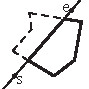
\includegraphics[width=\textwidth]{content/geometry/PolygonCut}
\vspace{-6mm}
\end{minipage}
 * Status: tested but not extensively
 * Usage:
 * 	vector<P> p = ...;
 * 	p = polygonCut(p, P(0,0), P(1,0));
 */

7d 7d #include "Point.h"
b1 c4 #include "lineIntersection.h"

6c 62 typedef Point<double> P;
f6 37 vector<P> polygonCut(const vector<P>& poly, P s, P e) {
2d fe 	vector<P> res;
26 d4 	rep(i,0,sz(poly)) {
30 21 		P cur = poly[i], prev = i ? poly[i-1] : poly.back();
f1 7b 		bool side = s.cross(e, cur) < 0;
00 bd 		if (side != (s.cross(e, prev) < 0))
37 9d 			res.push_back(lineInter(s, e, cur, prev).second);
0f e9 		if (side)
1d a5 			res.push_back(cur);
7a cb 	}
f3 b5 	return res;
75 cb }
\end{lstlisting}

\subsection{PolygonUnion.cpp}
\begin{lstlisting}
Hash: 6ab2ad
/**
 * Author: black_horse2014, chilli
 * Date: 2019-10-29
 * License: Unknown
 * Description: Calculates the area of the union of $n$ polygons (not necessarily
 * convex). The points within each polygon must be given in CCW order.
 * (Epsilon checks may optionally be added to sideOf/sgn, but shouldn't be needed.)
 * Status: stress-tested, Submitted on ECNA 2017 Problem A
 * Time: $O(N^2)$, where $N$ is the total number of points
 */

7d 7d #include "Point.h"
7e 12 #include "sideOf.h"

a8 62 typedef Point<double> P;
a7 14 double rat(P a, P b) { return sgn(b.x) ? a.x/b.x : a.y/b.y; }
15 61 double polyUnion(vector<vector<P>>& poly) {
c4 49 	double ret = 0;
f4 9a 	rep(i,0,sz(poly)) rep(v,0,sz(poly[i])) {
be 9c 		P A = poly[i][v], B = poly[i][(v + 1) % sz(poly[i])];
d8 05 		vector<pair<double, int>> segs = {{0, 0}, {1, 0}};
12 cb 		rep(j,0,sz(poly)) if (i != j) {
f1 cc 			rep(u,0,sz(poly[j])) {
c2 41 				P C = poly[j][u], D = poly[j][(u + 1) % sz(poly[j])];
db 68 				int sc = sideOf(A, B, C), sd = sideOf(A, B, D);
2c 68 				if (sc != sd) {
00 29 					double sa = C.cross(D, A), sb = C.cross(D, B);
a4 e9 					if (min(sc, sd) < 0)
fd da 						segs.emplace_back(sa / (sa - sb), sgn(sc - sd));
d8 0f 				} else if (!sc && !sd && j<i && sgn((B-A).dot(D-C))>0){
82 5b 					segs.emplace_back(rat(C - A, B - A), 1);
ed e9 					segs.emplace_back(rat(D - A, B - A), -1);
81 cb 				}
73 cb 			}
31 cb 		}
0e 86 		sort(all(segs));
e8 15 		for (auto& s : segs) s.first = min(max(s.first, 0.0), 1.0);
c2 68 		double sum = 0;
c7 72 		int cnt = segs[0].second;
1e 06 		rep(j,1,sz(segs)) {
2b 08 			if (!cnt) sum += segs[j].first - segs[j - 1].first;
eb 6e 			cnt += segs[j].second;
1a cb 		}
17 32 		ret += A.cross(B) * sum;
ca cb 	}
6a ad 	return ret / 2;
6a cb }
\end{lstlisting}

\subsection{SegmentDistance.cpp}
\begin{lstlisting}
Hash: a3104f
/**
 * Author: Ulf Lundstrom
 * Date: 2009-03-21
 * License: CC0
 * Source:
 * Description:\\
\begin{minipage}{75mm}
Returns the shortest distance between point p and the line segment from point s to e.
\end{minipage}
\begin{minipage}{15mm}
\vspace{-10mm}
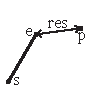
\includegraphics[width=\textwidth]{content/geometry/SegmentDistance}
\end{minipage}
 * Status: tested
 * Usage: 
 * 	Point<double> a, b(2,2), p(1,1);
 * 	bool onSegment = segDist(a,b,p) < 1e-10;
 */

7d 7d #include "Point.h"

d6 62 typedef Point<double> P;
a9 92 double segDist(P& s, P& e, P& p) {
1d a4 	if (s==e) return (p-s).dist();
5b f8 	auto d = (e-s).dist2(), t = min(d,max(.0,(p-s).dot(e-s)));
37 2c 	return ((p-s)*d-(e-s)*t).dist()/d;
a3 cb }
\end{lstlisting}

\subsection{SegmentIintersection.cpp}
\begin{lstlisting}
Hash: 12fa1d
/**
 * Author: Victor Lecomte, chilli
 * Date: 2019-04-27
 * License: CC0
 * Description:\\
\begin{minipage}{75mm}
If a unique intersection point between the line segments going from s1 to e1 and from s2 to e2 exists then it is returned.
If no intersection point exists an empty vector is returned. If infinitely many exist a vector with 2 elements is returned, containing the endpoints of the common line segment.
The wrong position will be returned if P is Point<ll> and the intersection point does not have integer coordinates.
Products of three coordinates are used in intermediate steps so watch out for overflow if using int or long long.
\end{minipage}
\begin{minipage}{15mm}
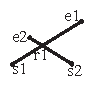
\includegraphics[width=\textwidth]{content/geometry/SegmentIntersection}
\end{minipage}
 * Status: Well tested with stress-test and with Kattis problem intersection.
 * Usage:
 * vector<P> inter = segInter(s1,e1,s2,e2);
 * if (sz(inter)==1)
 *   cout << "segments intersect at " << inter[0] << endl;
 */

7d 7d #include "Point.h"
94 8f #include "OnSegment.h"

68 da template<class P> vector<P> segInter(P a, P b, P c, P d) {
f9 0b 	auto oa = c.cross(d, a), ob = c.cross(d, b),
1a 31 	     oc = a.cross(b, c), od = a.cross(b, d);
      	// Checks if intersection is single non-endpoint point.
c8 91 	if (sgn(oa) * sgn(ob) < 0 && sgn(oc) * sgn(od) < 0)
f5 e5 		return {(a * ob - b * oa) / (ob - oa)};
3b 4c 	set<P> s;
d5 cc 	if (onSegment(c, d, a)) s.insert(a);
35 0a 	if (onSegment(c, d, b)) s.insert(b);
93 3d 	if (onSegment(a, b, c)) s.insert(c);
be 2f 	if (onSegment(a, b, d)) s.insert(d);
e4 a3 	return {all(s)};
12 cb }
\end{lstlisting}

\subsection{SideOf.cpp}
\begin{lstlisting}
Hash: f459d8
/**
 * Author: Ulf Lundstrom
 * Date: 2009-03-21
 * License: CC0
 * Source:
 * Description: Returns where $p$ is as seen from $s$ towards $e$. 1/0/-1 $\Leftrightarrow$ left/on line/right. If the optional argument $eps$ is given 0 is returned if $p$ is within distance $eps$ from the line. P is supposed to be Point<T> where T is e.g. double or long long. It uses products in intermediate steps so watch out for overflow if using int or long long.
 * Status: tested
 * Usage:
 * 	bool left = sideOf(p1,p2,q)==1;
 */

7d 7d #include "Point.h"

07 7d template<class P>
14 70 int sideOf(P s, P e, P p) { return sgn(s.cross(e, p)); }

54 7d template<class P>
d4 b5 int sideOf(const P& s, const P& e, const P& p, double eps) {
c3 79 	auto a = (e-s).cross(p-s);
37 65 	double l = (e-s).dist()*eps;
4a c3 	return (a > l) - (a < -l);
f4 cb }
\end{lstlisting}

\subsection{SortByAngle.cpp}
\begin{lstlisting}
Hash: e2a0d7
/**
 * Author: Tiago
 * Date: 2021-02-14
 * Description:
  Sort points by angle arround a chosen pivot, untied by distance
 * Time: O(n \log n)
*/

f3 f3 	sort(all(pts) , [&](P a , P b){
c0 05 		a = a - pivot , b = b - pivot;
7e c0 		int hp1 = a < P(0,0) , hp2 = b < P(0,0);
2a 07 		if(hp1 != hp2) return hp1 < hp2;
4f 48 		if(a.cross(b) != 0){
fa c3 			return a.cross(b)  > 0;
46 cb 		}
3f ba 		return a.dist2() < b.dist2();
e2 c0 	});
\end{lstlisting}

\pagebreak


%%%%%%%%%%%%%%%%%%%%
%
% Extra
%
%%%%%%%%%%%%%%%%%%%%

\section{Extra}

\end{document}
